%% For Cambridge soft-bound version
\documentclass[hyperpdf,bindnopdf]{hepthesis}

%% For Cambridge hard-bound version (must be one-sided)
%\documentclass[hyperpdf,oneside]{hepthesis}

%% Load special font packages here if you wish
%\usepackage{lmodern}

\usepackage{mathpazo}
\usepackage{amsmath}
\usepackage{enumerate}
\usepackage{tabularx}
\usepackage{notoccite}
\usepackage{rotating}
\usepackage{lscape}
\usepackage{titlepic}
\usepackage{graphicx}
\usepackage{listings}
\lstset{
	basicstyle=\ttfamily,
	frame=single,
	basewidth  = {.5em,0.5em},
	basicstyle=\linespread{0.6},
	breaklines=true
}
%\usepackage{euler}
%% Put package includes etc. into preamble.tex for convenience
\usepackage{xspace}
\usepackage{tikz}
\usepackage{morefloats,subfig,afterpage}
\usepackage{mathrsfs} % script font
\usepackage{verbatim}
\usepackage{adjustbox}
\usepackage{multirow}
%% Using Babel allows other languages to be used and mixed-in easily
%\usepackage[ngerman,english]{babel}
\usepackage[english]{babel}
\selectlanguage{english}

%% Citation system tweaks
\usepackage{cite}
% \let\@OldCite\cite
% \renewcommand{\cite}[1]{\mbox{\!\!\!\@OldCite{#1}}}

%% Maths
% TODO: rework or eliminate maybemath
\usepackage{abmath}
\DeclareRobustCommand{\mymath}[1]{\ensuremath{\maybebmsf{#1}}}
% \DeclareRobustCommand{\parenths}[1]{\mymath{\left({#1}\right)}\xspace}
% \DeclareRobustCommand{\braces}[1]{\mymath{\left\{{#1}\right\}}\xspace}
% \DeclareRobustCommand{\angles}[1]{\mymath{\left\langle{#1}\right\rangle}\xspace}
% \DeclareRobustCommand{\sqbracs}[1]{\mymath{\left[{#1}\right]}\xspace}
% \DeclareRobustCommand{\mods}[1]{\mymath{\left\lvert{#1}\right\rvert}\xspace}
% \DeclareRobustCommand{\modsq}[1]{\mymath{\mods{#1}^2}\xspace}
% \DeclareRobustCommand{\dblmods}[1]{\mymath{\left\lVert{#1}\right\rVert}\xspace}
% \DeclareRobustCommand{\expOf}[1]{\mymath{\exp{\!\parenths{#1}}}\xspace}
% \DeclareRobustCommand{\eexp}[1]{\mymath{e^{#1}}\xspace}
% \DeclareRobustCommand{\plusquad}{\mymath{\oplus}\xspace}
% \DeclareRobustCommand{\logOf}[1]{\mymath{\log\!\parenths{#1}}\xspace}
% \DeclareRobustCommand{\lnOf}[1]{\mymath{\ln\!\parenths{#1}}\xspace}
% \DeclareRobustCommand{\ofOrder}[1]{\mymath{\mathcal{O}\parenths{#1}}\xspace}
% \DeclareRobustCommand{\SOgroup}[1]{\mymath{\mathup{SO}\parenths{#1}}\xspace}
% \DeclareRobustCommand{\SUgroup}[1]{\mymath{\mathup{SU}\parenths{#1}}\xspace}
% \DeclareRobustCommand{\Ugroup}[1]{\mymath{\mathup{U}\parenths{#1}}\xspace}
% \DeclareRobustCommand{\I}[1]{\mymath{\mathrm{i}}\xspace}
% \DeclareRobustCommand{\colvector}[1]{\mymath{\begin{pmatrix}#1\end{pmatrix}}\xspace}
\DeclareRobustCommand{\Rate}{\mymath{\Gamma}\xspace}
\DeclareRobustCommand{\RateOf}[1]{\mymath{\Gamma}\parenths{#1}\xspace}

%% High-energy physics stuff
\usepackage{abhep}
\usepackage{hepnames}
\usepackage{hepunits}
\DeclareRobustCommand{\arXivCode}[1]{arXiv:#1}
\DeclareRobustCommand{\CP}{\ensuremath{\mathcal{CP}}\xspace}
\DeclareRobustCommand{\CPviolation}{\CP-violation\xspace}
\DeclareRobustCommand{\CPv}{\CPviolation}
\DeclareRobustCommand{\LHCb}{LHCb\xspace}
\DeclareRobustCommand{\LHC}{LHC\xspace}
\DeclareRobustCommand{\LEP}{LEP\xspace}
\DeclareRobustCommand{\CERN}{CERN\xspace}
\DeclareRobustCommand{\bphysics}{\Pbottom-physics\xspace}
\DeclareRobustCommand{\bhadron}{\Pbottom-hadron\xspace}
\DeclareRobustCommand{\Bmeson}{\PB-meson\xspace}
\DeclareRobustCommand{\bbaryon}{\Pbottom-baryon\xspace}
\DeclareRobustCommand{\Bdecay}{\PB-decay\xspace}
\DeclareRobustCommand{\bdecay}{\Pbottom-decay\xspace}
\DeclareRobustCommand{\BToKPi}{\HepProcess{ \PB \to \PK \Ppi }\xspace}
\DeclareRobustCommand{\BToPiPi}{\HepProcess{ \PB \to \Ppi \Ppi }\xspace}
\DeclareRobustCommand{\BToKK}{\HepProcess{ \PB \to \PK \PK }\xspace}
\DeclareRobustCommand{\BToRhoPi}{\HepProcess{ \PB \to \Prho \Ppi }\xspace}
\DeclareRobustCommand{\BToRhoRho}{\HepProcess{ \PB \to \Prho \Prho }\xspace}
\DeclareRobustCommand{\X}{\thesismath{X}\xspace}
\DeclareRobustCommand{\Xbar}{\thesismath{\overline{X}}\xspace}
\DeclareRobustCommand{\Xzero}{\HepGenParticle{X}{}{0}\xspace}
\DeclareRobustCommand{\Xzerobar}{\HepGenAntiParticle{X}{}{0}\xspace}
\DeclareRobustCommand{\epluseminus}{\Ppositron\!\Pelectron\xspace}
\DeclareRobustCommand{\protonproton}{\Pproton\APantiproton\xspace}
\DeclareRobustCommand{\met}{E_{T}^{miss}}
\DeclareRobustCommand{\pt}{p_{T}}
\DeclareOldFontCommand{\bf}{\normalfont\bfseries}{\mathbf}
\DeclareOldFontCommand{\rm}{\normalfont\rmfamily}{\mathrm}
\DeclareOldFontCommand{\sf}{\normalfont\sffamily}{\mathsf}
\DeclareOldFontCommand{\tt}{\normalfont\ttfamily}{\mathtt}
\DeclareOldFontCommand{\bf}{\normalfont\bfseries}{\mathbf}
\DeclareOldFontCommand{\it}{\normalfont\itshape}{\mathit}
\DeclareOldFontCommand{\sl}{\normalfont\slshape}{\@nomath\sl}
\DeclareOldFontCommand{\sc}{\normalfont\scshape}{\@nomath\sc}
\DeclareRobustCommand*\cal{\@fontswitch\relax\mathcal}
\DeclareRobustCommand*\mit{\@fontswitch\relax\mathnormal}


%% You can set the line spacing this way
%\setallspacing{double}
%% or a section at a time like this
%\setfrontmatterspacing{double}


%% Define the thesis title and author
\title{Searches for Diboson New Physics and the L1Calo Software Development with the ATLAS detector}
\author{Chiao-Ying Lin}


%% Doc-specific PDF metadata
\makeatletter
\@ifpackageloaded{hyperref}{%
	\hypersetup{%
		pdftitle = {Searches for Diboson New Physics and the L1Calo Software Development with the ATLAS Detector},
		pdfsubject = {Chiao-Ying Lin's PhD thesis},
		pdfkeywords = {ATLAS, Diboson, electroweak, exotics, Standard Model, DAQ, Trigger, L1Calo},
		pdfauthor = {\textcopyright\ Chiao-Ying, Lin}
}}{}
\makeatother

%% Start the document
\begin{document}

	%% Define the un-numbered front matter (cover pages, rubrik and table of contents)
\begin{frontmatter}
    %% Title
%\titlepage[of Peterhouse]{./Peterhouse.png}{
%  A dissertation submitted to the University of Cambridge\\ for the degree of Doctor of Philosophy}
%% Abstract
\begin{center}%
	%\vspace*{\frontmattertitleskip}%
	\begin{doublespace}%
		{\Huge\textbf{\thetitle}}\\%
	\end{doublespace}%
	\vspace*{3cm}%
	{\Large{\theauthor} \\ of Peterhouse }\\%
	\vspace*{3cm}%
	
\includegraphics[width=5cm]{Peterhouse.png} \\
	\vspace*{2cm}
	{A thesis submitted to the University of Cambridge\\ for the degree of Doctor of Philosophy \\ Aug 2019}
\end{center}%
\begin{abstract}%[\smaller \thetitle\\ \vspace*{1cm} \smaller {\theauthor}]
  %\thispagestyle{empty}
The Standard Model has been a successful theory in describing the behaviour of fundamental particles, but there are still problems remaining unsolved. New theoretical models are therefore proposed to answer those questions with either new interactions or new particles. This thesis is presenting the searches for new physics with diboson signatures in these two ways from LHC $\sqrt{s}=13~TeV$ collisions with the ATLAS detector with the data collected in 2015 and 2016 corresponding to an integrated luminosity of $36.1~fb^{-1}$. The searching strategy was performed with the Monte Carlo simulation for the SM background modelling and a data-driven method for the multijet background estimation. The final result was interpreted by a comparison between background modelling and data by a CLs method. For the resonance search, no new particle was discovered, and mass limits are therefore set on the new particles from models taken as the interpretation benchmarks. For the study on new interactions in the signatures of vector boson scattering, the first measurement of this process with the semileptonic decay was given with a significance of $2.7\sigma$ in reasonable agreement with the SM prediction
\\
\\Both the LHC and ATLAS detector are now going through the upgrades for operations in 2021 with the $\sqrt{s}=14~TeV$ collisions. The ATLAS hardware calorimeter trigger is part of the upgrade project for the implementation of three new object processors: eFex, jFex, and gFex. This thesis will also present the construction of simulation system along with the expected performance of proposed object reconstruction algorithms for this new infrastructure.

\end{abstract}
%% Declaration
\begin{declaration}
  This thesis is the result of my own work, except where explicit
reference is made to the work of others, and has not been submitted
for another qualification to this or any other university. This
thesis does not exceed the word limit for the respective Degree
Committee.
  \vspace*{1cm}
  \begin{flushright}
    Chiao-Ying Lin
  \end{flushright}
\end{declaration}


%% Acknowledgements
\begin{acknowledgements}
\noindent
The three and half years of PhD has been a wonderful adventure, and here is to present my appreciation for the people who are part of my journey.
\\
\\Firstly, I want to thank my supervisor, Christopher Lester. The whole work of my PhD will not be possible without his support and help. And, I also want to show my gratitude to my college, Peterhouse, for funding my PhD and enriching my life out of research. 
\\
\\Then, I would like to thank Takuya Nobe, Viviana Cavaliere, and Lailin Xu as the convenors for the analysis works I was involved in. Those tasks are complicated like a maze, and they provide the guidance to show where is the way to go to have the final results. I would also like to thank Ben Carlson for all my L1Calo works, because I cannot keep working on the L1Calo upgrade project without his support.  I also want to present my appreciation to John Chapman, John Hill, and Will Buttinger for all the helps on the technical problems I encountered when dealing with varied software tools.
\\
\\For my social life during PhD, I am glad to be part of the friendly Cambridge HEP group, and I want to thank everyone in the group for the sweet tea time and nice chats. Especially, I want to thank James Cowley, Alison Tully, Ben Brunt, Jonathan Rostén, Holly Pacey, and Herschel Chawdhry for the company. They have made the research work not so intense, as I can always have fun with those people. I also want to say thank you to the Cambridge Taiwanese Society, especially Cheng-Tai Lee, because this is where I can still keep the connection to where I am from even though I am thousands of miles away from home. Most importantly, I can get rid of the stress by complaining in my mother tongue with those people.
\\
\\For the last part of this list, I would like to thank my family for supporting me to be away for the pursuit of this degree. 

\end{acknowledgements}



%% ToC
\tableofcontents


%% Strictly optional!
\frontquote{%
  We are just an advanced breed of monkeys on a minor planet of a very average star. But we can understand the Universe. That makes us something very special.}%
  {Stephen Hawking}
%% I don't want a page number on the following blank page either.
\thispagestyle{empty}

\end{frontmatter}
	
	%% Start the content body of the thesis
\begin{mainmatter}
	\begin{spacing}{1.4}
    \chapter{Introduction and Motivation}
Particle physics is the subject to study the fundamental structure of the universe. It is now based on the theory called the "Standard Model" (SM). It interprets the universe as the composition of tiny particles interacting with each other by the exchange of force carriers (another type of particle).  In July 2012, the discovery of Higgs boson made by the ATLAS and CMS collaboration completed SM 50 years after being predicted. By now, it has been deemed as one of the most successful theories in modern physics.
\\
\\
However, there are still some conflicts between the SM and factual results. For example, in the SM, neutrinos are supposed to be massless, but the discovery of neutrino oscillation support the fact that neutrinos are massive, and the SM cannot explain it. New theories are proposed in order to resolve those conflicts, and they indicate the existence of some new particles or the deviation from SM predictions. This thesis is dedicated to the work in search for this kind of new physics.  
\section{Standard Model}
The SM is a quantum field theory(QFT). In a QFT the universe is filled with different fields, and all fundamental particles (particles without further substructure) are the forms of quantized fields. They make up the matters and also mediate interactions between them, which is the foundation how this universe operates. Those fundamental particles could be classified into two types: fermions and bosons. Fermions are the matter builders, while bosons are the force carriers exchanged between particles (for both fermions and bosons). 
\\
\\{\bf Fermions}
\\
\\Fermions are quantized from fermionic fields following Dirac-Fermi statistics with half integer spin number, $\pm\frac{1}{2}$. Under the statistic characteristic, fermions exclude each other with the same quantum status, which makes them different from bosons. \\
\\
All fermions have their counter antiparticles which in the SM have opposite charge and chirality. Those fermions are called "Driac Fermions". They can be presented as Weyl spinors of four components composed of one left-handed spinor and one right handed spinor following the Dirac equation. However, neutrinos, a sub-specie of fermions, have no counter-partner with opposite chirality found\footnote{Due to being neutral, although neutrinos and anti-neutronos were discovered, but neutrinos (anti-neutrinos) only have the left-handed (right-handed) chirality.}, so they are assumed to be "Majorana Fermions": they are their own antiparticle. They could be instead presented as Majorana spinors in Majorana equation. 
\\
\\{\bf Dirac Equation}: $i\hbar\gamma^{\mu}\partial_{\mu}\psi-mc\psi=0$ 
\\
\\{\bf Majorana Equation}: $i\hbar\gamma^\mu\partial_\mu\psi-mc\psi_c=0$
\\
\\$\psi$ is the fermion field with charge conjugate $\psi_c$, and $\gamma^\mu$ is the gamma matrix and m is the particle mass.
\\ 
\\Fermions can then be further categorized into two types, quarks and leptons, by the interactions they participate in. Quarks are the only particles involved in the strong interaction, so they cannot exist alone, and, instead, they are always in bound state as mesons of two quarks or baryons of three quarks. 
\\
\\Quarks have three generations (flavours) and six flavours. In each generation are quarks with different charges: $\frac{-1}{3}$ and $\frac{2}{3}$. The first generation are the lightest: up and down. Strange and charm are in the second generation. The third generation has bottom and top with highest mass. Quarks can change their flavour through CKM matrix relating to the weak interaction. The decay relation between quarks is shown in Fig.\ref{Fig:quarks}
\\    
\begin{figure}[!h]                
	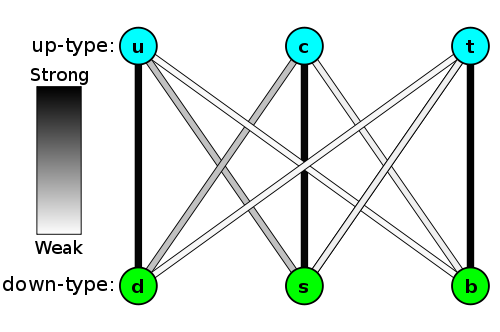
\includegraphics[width=0.45\textwidth]{Chapter1/quarks.png}
	\centering
	\begin{center}
		\caption{Relation between quarks are determined by CKM matrix.}
		\label{Fig:quarks}            
	\end{center}
\end{figure}

Similar to quarks, leptons also have 3 generations and 6 flavours. In each generation, there is one neutral neutrino and corresponding charged particle with charge -1. The three generations are electrons, muons and taus with their neutrino partners (among them, electron neutrino is assumed to be the lightest fundamental particle under normal hierarchy). Leptons participate in weak interaction, quantum electrodynamics(except for neutral neutrinos) and gravity. They can change flavours through PMNS matrix relating to the weak interaction.
\\
\\{\bf Interaction and Bosons}
\\
\\Under the SM, the interactions between particles are induced by gauge fields which could be quantized into gauge bosons. Different from fermions, those bosons follow Bose-Einstein statistics with integer spin number, which means more than one is allowed to occupy a single quantum state. They mediate interactions between particles including themselves. 
\\
\\Although there are four fundamental forces in the universe, only three of them are in SM, because they are quantizable: electromagnetic, weak and strong interactions. The challenge of quantizing gravity is still not achieved in modern physics. Each interaction has a part in the SM Lagrange formulism.
\\
\\The electromagnetic interaction is the best known among the four interactions. It is explained by quantum electrodynamics in the SM. The interaction is induced by electromagnetic field between two charged particles with charge as the invariance under $U(1)$ symmetry, which could be seen as they interchange photons. Because the electromagnetic interaction only occurs between charged particles, photon doesn't interact with neutral particles at the leading order \footnote{With a loop diagram, it can still be achieved by exchanging charged fermions between photons.}. The coupling constant (interaction strength which determines the possibility of a process  occurs) in the interaction is:
\\
\begin{equation}
\alpha_{EM} = \frac{e^2}{4\pi\hbar c}=\frac{1}{137.036...}
\end{equation}
\\
with $e$ as electric charge of electron, $\hbar$ as reduced Plank constant and $c$, the speed of light. Its part in the SM Lagrange could be written as:
\begin{equation}
\mathcal{L}=\bar{\psi}(i\gamma^{\mu}D_{\mu})\psi-F^{\mu\nu}F_{\mu\nu}
   \label{Eq:EM Lagrange}  
\end{equation}
In this equation, $\gamma^\mu$ is the Gamma matrices, $\psi$ is the Weyl spinor of spin $-\frac{1}{2}$ particles and $\bar{\psi}$ is the Dirac adjoint of $\psi$. $D_\mu=\partial_\mu+ieA_\mu+ieB_\mu$ represents the gauge covariant derivative with $e$ as the electric charge, $A_\mu$ as the filed induced by the particle itself and $B_\mu$ as the field from external source. In the equation, $F_{\mu\nu}$ is the electromagnetic field tensor. 
\\
\\All the left-handed particles participate in the weak interaction. It is mediated by three different bosons: the $W^+$, $W^-$ and $Z^0$ bosons. They are massive gauge bosons which obtain their mass via the electroweak symmetry breaking. The W boson is the mediator when a particle changes its flavour along with its charge, while Z boson is involved in the neutral current interactions which leave the particles unchanged with only kinematic momentum transfer. Within this process, a quantity, isospin, is conserved under $SU_L(2)$ symmetry. Its definition is similar to the spin numbers of a pair of electrons in the same orbital. For two fermions in the same generations, their quantum states are identical except for isospin which is opposite of them to each other. As right-handed fermions don't participate in weak interaction, their isospin is 0. The isospins of fermions are showed in Table.\ref{Tab:isospin}. 
\\


\begin{table}[h]
	\caption{Isospin of Elementary fermions}
	\renewcommand{\arraystretch}{1.2}
	\centering
	\begin{tabular}{l c c c c r}
		\hline
		\hline
		1st Generation &Isospin        &2nd Generation    &Isospin        &3rd Generation   &Isospin\\
		\hline
		$e^-$          &$-\frac{1}{2}$ &$\mu^-$           &$-\frac{1}{2}$ &$\tau$           &$-\frac{1}{2}$\\
		\hline
		$\nu_e$        &$\frac{1}{2}$  &$\nu_\mu$         &$\frac{1}{2}$  &$\nu_\tau$       &$\frac{1}{2}$\\
		\hline
		$u$            &$\frac{1}{2}$  &$c$               &$\frac{1}{2}$  &$t$              &$\frac{1}{2}$\\
		\hline
		$d$            &$-\frac{1}{2}$ &$s$               &$-\frac{1}{2}$ &$b$              &$-\frac{1}{2}$\\
		\hline

	\end{tabular}
    \label{Tab:isospin}
\end{table}
\noindent
The coupling constant for weak interaction is defined as:
\begin{equation}
\alpha_{W} = \frac{g_{W}}{4\pi\hbar c}\approx\frac{1}{29}
\end{equation}
with $g_{W}$ as the W weak charge strength. In terms of the interactions via Z boson, it is substituted by Z weak charge, $g_{Z}$. A unification between the weak and electromagnetic interactions could be achieved with another new parameter called electroweak hypercharge defined as $Y_w=2 (Q-I_3)$ where $I_3$ is isospin and $Q$ is the electric charge under $SU_L(2)\times U(1)$ symmetry in the scale of high energy.  In SM, the symmetry would be spontaneously broken by the Higgs field to give particles mass. It will be discussed in the next section.
\\
\\Only quarks are involved in the strong interaction which is described by quantum chromodynamics(QCD). The conserved quantity in the interaction is also imaginary, colour, with gluons as the force carrier boson under $SU(3)$ symmetry. There are three different colours: red, blue and green along with their anti-colour partners. Similar to the principle of light, the colour would be absent when the three colours are mixed together or with their anti-colour, and it is the condition for a stable state in QCD. Each quark is only allowed to carry one colour, but this state is unstable. It needs to be bound with another quarks to stabilize the system, and they exchange gluons to form the bounding force. In QCD, gluons have 8 types with different colour combinations:
\begin{equation}
         (r\bar{b}+b\bar{r})/\sqrt{2}, \quad -i(r\bar{b}-b\bar{r})/\sqrt{2}  \\
         (r\bar{g}+g\bar{r})/\sqrt{2}, \quad -i(r\bar{g}-g\bar{r}/\sqrt{2})  \\
          (b\bar{g}+g\bar{b})/\sqrt{2},\quad -i(b\bar{g}-g\bar{b}/\sqrt{2})   \\
          (r\bar{r}-b\bar{b})/\sqrt{2},\quad  (r\bar{r}+b\bar{b}-2g\bar{g})/\sqrt{6}
\end{equation}
with $r$, red charge, $b$, blue charge, and $g$, green charge.
\\
\\Different from the other interactions, the colour confinement of gluon self-interaction makes the effective potential increase linearly with the distance between two colour-charged particles. Under this process, the potential energy decays into a quark-antiquark pair, and it is repeated also within the newly produced pair. This leads to the divergence of with the perturbative strong coupling constant, and the mathematical technique, ``renormalization'', is introduced to solve the problem. 
\\
\\Its part of the SM Lagrange could be shown as:
\begin{equation}
\mathcal{L}_{QCD}=\bar{\psi}(i(\gamma^\mu D_\mu)_{ij}-m\delta_{ij})\psi_j-\frac{1}{4}G^a_{\mu\nu}G_a^{\mu\nu} 
\end{equation}
with
\begin{equation}
G^a_{\mu\nu}=\partial_\mu\mathcal{A}^a_\mu-\partial_\nu\mathcal{A}^a_\nu+gf^{abc}\mathcal{A}^b_\mu\mathcal{A}^c_\nu 
\end{equation}
with $\psi_i$, the quark field in $SU(3)$ representation indexed of i,j, ..., $G^a_{\mu\nu}$, the gluon field also in $SU(3)$ representation indexed of a, b... from 1 to 8. $f^{abc}$ is the structure constant, $\mathcal{A}_\mu$ is the spin 1 gluon filed and $g = \sqrt{4\pi\alpha_s}$ is the QCD coupling constant.
\\
\\All the elementary particles with their basic properties are shown in Fig. \ref{Fig:elementary_particle}. The 3 interactions with their conserved quantities makes SM under the gauge theory with the gauge group with $U(1) \times SU(2)_L \times SU(3)$ gauge group.

\begin{figure}[!h]                
	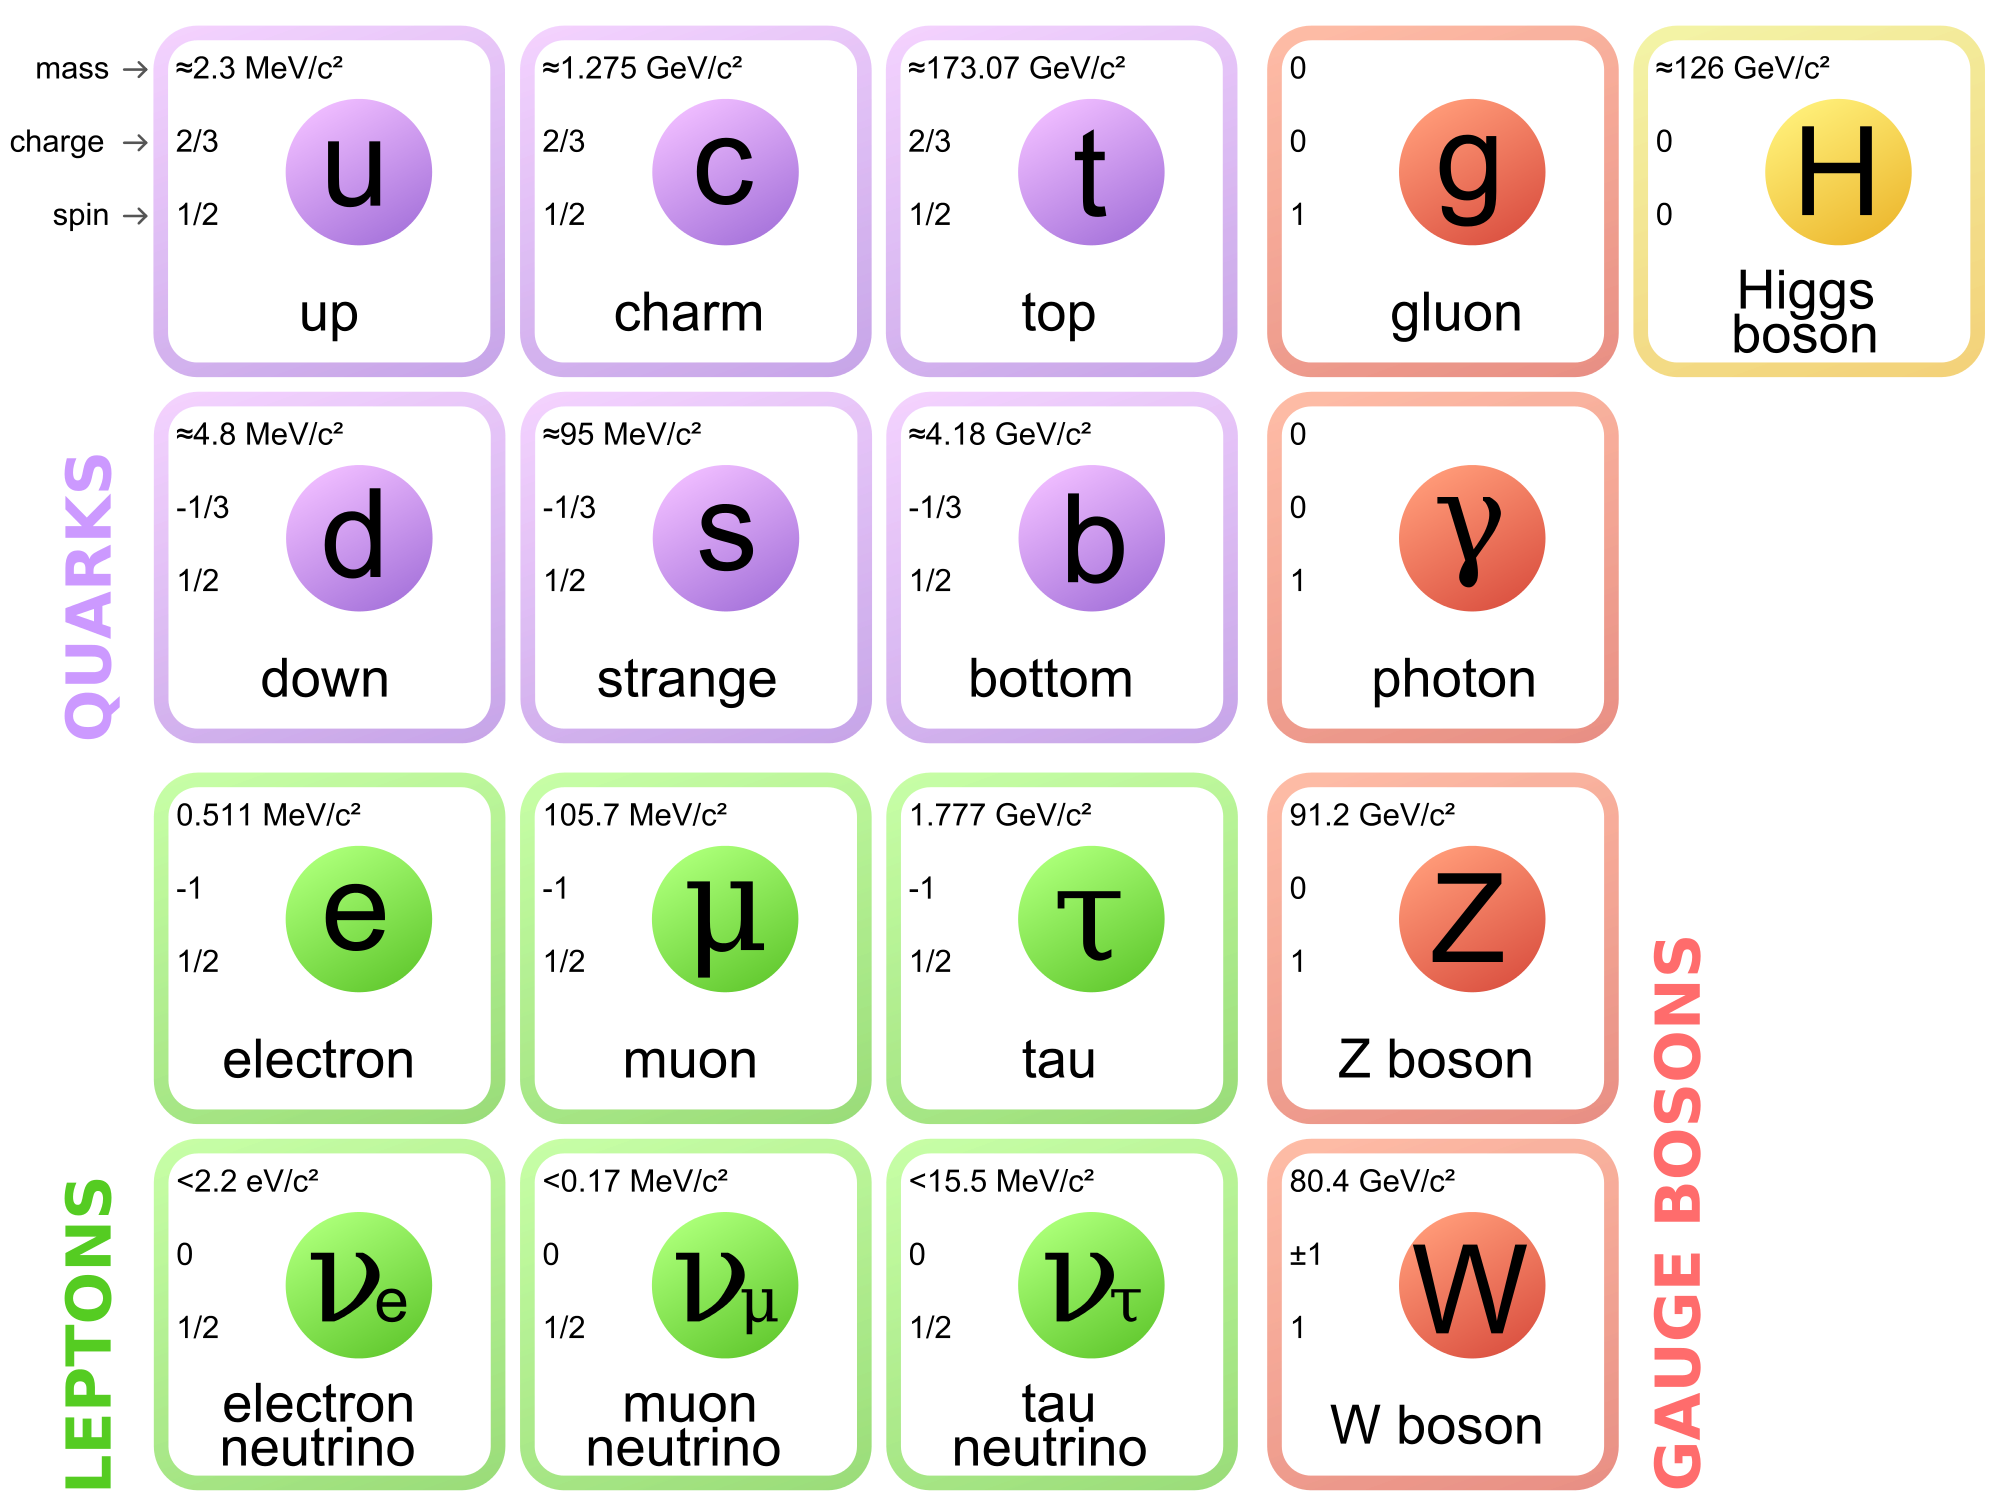
\includegraphics[width=0.9\textwidth]{Chapter1/elementary_particle.png}
	\centering
	\begin{center}
		\caption{Elementary particles and properties}
		\label{Fig:elementary_particle}            
	\end{center}
\end{figure}

\section{Electroweak Symmetry Breaking}
One particle in Fig. \ref{Fig:elementary_particle} is not mentioned yet: Higgs boson, the last discovered fundamental particle in the SM. It 
arises from quantized Higgs field which was proposed by three groups in early 1960s:  Robert Brout and Francois Englert, Peter Higgs as well as Gerald Guralnik, C. R. Hagen, and Tom Kibble. It induces spontaneous electroweak symmetry breaking via the ''Brout-Englert-Higgs mechanism``.  The Higgs boson discovery was announced on 4th July 2012 and confirmed on 14 March 2013 with spin 0 and $+$ parity by the ATLAS and CMS collaboration.
\\
\\The Higgs field is defined as the scalar gauge field in a complex scalar $SU(2)_L$ doublet :
\begin{equation}
 \Phi= \left(  \begin{array}{ c } \phi^+\\  \phi^0 \end{array} \right) 
\end{equation}
The potential for field is:
\begin{equation}
 V(\Phi)=\mu^2|\Phi^\dagger\Phi|+\lambda(|\Phi^\dagger\Phi|)^2
\label{Eq:sm_higgs_potential}
\end{equation}
For some value of $\mu$ and $\lambda$, the minimal potential can be at $\Phi = 0$, and the shape of the potential would be as Fig. \ref{Fig:V} (this is a simplified plot, and the real one should be in 4 dimensions). In this potential, the symmetry is not broken with the minimal value at $\Phi = 0$.
\\ 
\begin{figure}[!h]                
	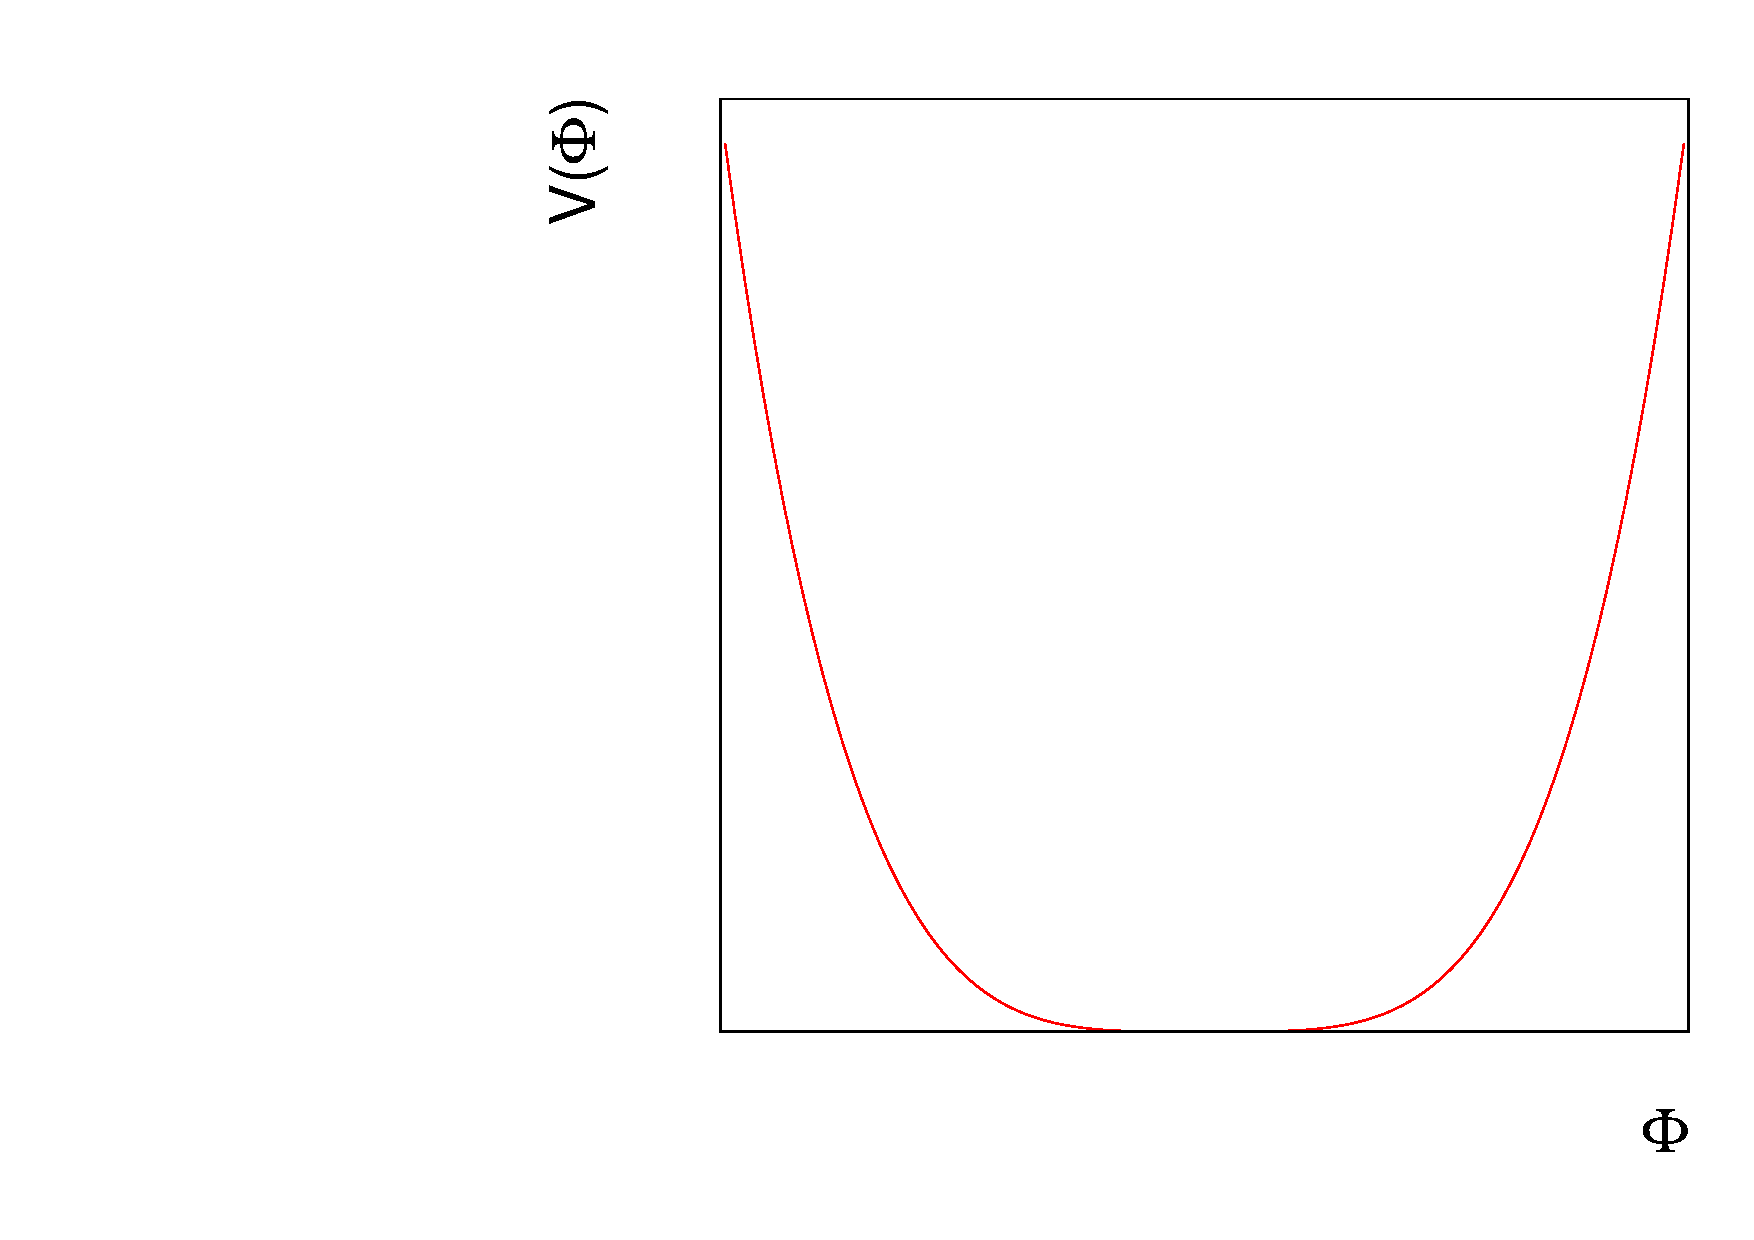
\includegraphics[width=0.4\textwidth]{Chapter1/V.pdf}
	\centering
	\begin{center}
		\caption{Scalar potential with $\mu^2 > 0$}
		\label{Fig:V}            
	\end{center}
\end{figure}
\\In an alternative scenario for $\mu^2 < 0$, the potential shape becomes Fig. \ref{Fig:higgs}. The minimal expected value of the potential is not at 0 but at:
\begin{equation}
\label{Eq:min}
\langle\Phi\rangle=\sqrt{-\frac{\mu^2}{2\lambda}}\left ( \begin{array}{c} 0 \\ 1 \end{array} \right) \equiv\frac{\nu}{\sqrt{2}}\left ( \begin{array}{c} 0 \\ 1 \end{array} \right)
\end{equation}
The potential is only affected by $|\Phi^\star\Phi|$, so the shape of the potential is determined by the real term (imaginary terms are cancelled out). The value in Eq.~\ref{Eq:min} is called the "vacuum expectation value"(VEV). To maintain a stable state, particles are only allowed to stay in the lowest potential, the valley part. This makes the degree of freedom of the particles decrease from four to one and breaks the $SU_L(2)\times U(1)$ symmetry with isospin and hypercharge to $U(1)$ symmetry with electric charge.  
\begin{figure}[!h]                
	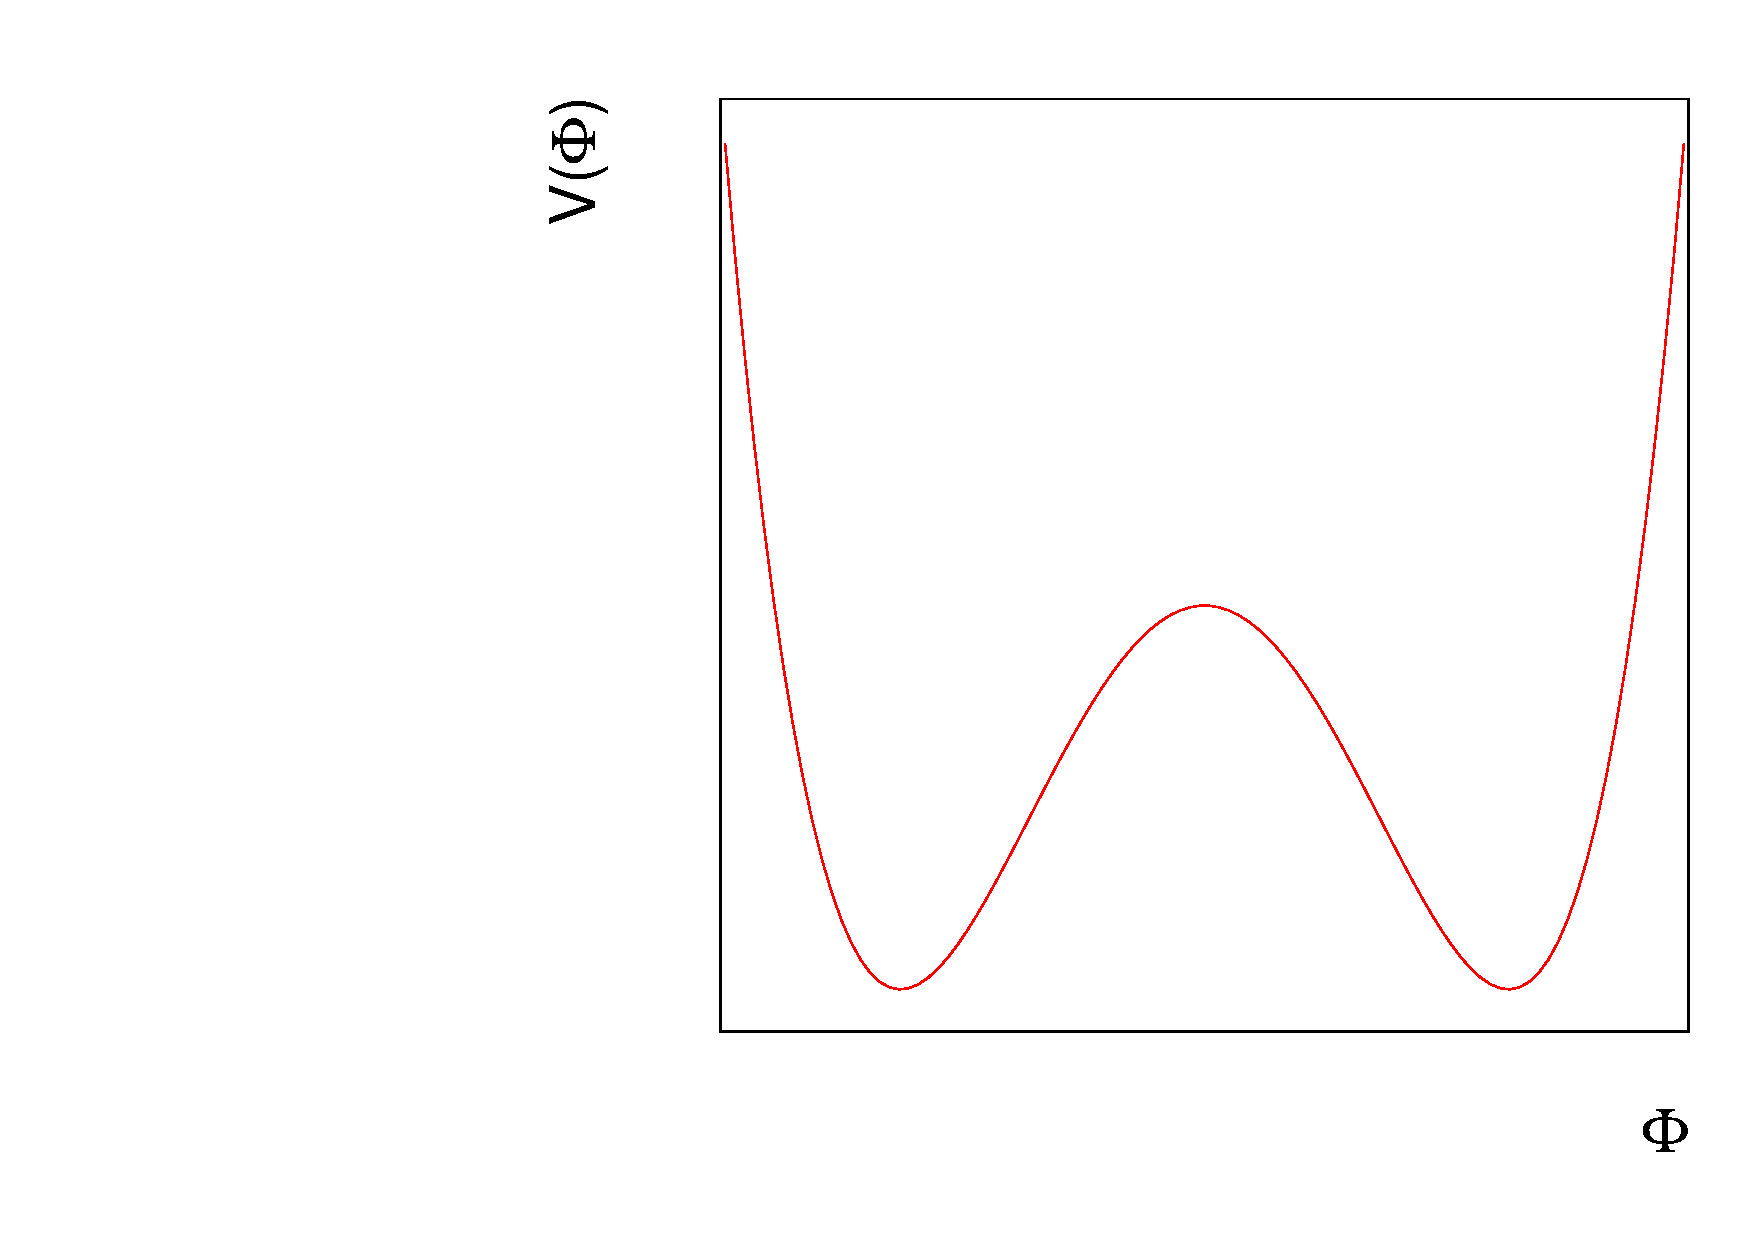
\includegraphics[width=0.4\textwidth]{Chapter1/higgs.pdf}
	\centering
	\begin{center}
		\caption{Scalar potential with $\mu^2 < 0$}
		\label{Fig:higgs}            
	\end{center}
\end{figure}
In high energy regime above the valley (excited state), electromagnetic and weak interaction are mixed together to form three $SU_L(2)$ gauge bosons, $W^i_\mu$ with $\mu =1,2,3$ and one $U(1)$ gauge boson, $B_\mu$. They are not SM particles, but they could be taken as the excited form of SM gauge bosons. The Lagrangian for the interaction between them and Higgs field is:
\begin{equation}
 \mathcal{L}=(D^\mu\Phi)^\dagger(D_\mu\Phi) - V(\Phi) 
\end{equation}
with
\begin{equation}
 D_\mu = \partial_\mu+i\frac{g}{2}\tau\cdot W_\mu+i\frac{g'}{2}B_\mu Y
 \label{Eq:electroweak symmetry Lagrange}  
\end{equation}
$g$ and $g'$ are the coupling constants between the fields, $\tau$ is the Pauli matrix and Y is the hypercharge.
\\
\\A unitary gauge transformation on the Higgs field can remove Goldstone bosons\footnote{Unitary gauge transformation is to select the fixed gauge which sets the Goldstone boson terms into 0} after the symmetry breaking. The Higgs field is thus shifted with the new gauge as:
\begin{equation}
\Phi=\frac{\nu+h}{\sqrt{2}}\left ( \begin{array}{c} 0 \\ 1 \end{array} \right)
\end{equation}
with h, the physical Higgs sector, as a complex number.
\\
\\After inserting the new Higgs field into and rearranging SM Lagrange, the SM gauge bosons could be shown as:  
\begin{equation}
W^{\pm}_\mu=\frac{1}{\sqrt{2}}(W^{1}_\mu\mp iW^{2}_\mu) 
\end{equation}
\begin{equation}
Z^\mu=\frac{-g'B_\mu+gW^3_\mu}{\sqrt{g^2+g'^2}} 
\end{equation}
\begin{equation}
A^\mu=\frac{gB_\mu+g'W^3_\mu}{\sqrt{g'^2+g^2}} 
\end{equation}
with particle masses:
\begin{equation}
M^2_W=\frac{1}{4}g^2\nu^2 
\end{equation}
\begin{equation}
M^2_Z =\frac{1}{4}(g^2+g'^2)\nu^2 
\end{equation}
\begin{equation}
M_A=0 
\end{equation}
From the expression, it turns out that $Z$ boson and photon are both the mix of $B$ and $W^3$ bosons with different phases which could be shown as:
\begin{equation}
 \left[ \begin{array}{c}  A \\ Z \end{array} \right]=\left[ \begin{array}{l r} cos\theta_W &  sin\theta_W \\ -sin\theta_W & cos\theta_W \end{array} \right]\left[ \begin{array}{c}  B\\ W^3 \end{array} \right] 
  \label{Eq:AZ phase}  
\end{equation}
With $\cos{\theta_W}=\frac{g}{\sqrt{g^2+g'^2}}$ and $\sin{\theta_W}=\frac{g'}{\sqrt{g^2+g'^2}}$. Here, $\theta_W$ is called the weak mixing angle or Weinberg angle. By this, the electroweak parameter, $\rho$, is defined:
\begin{equation}
\label{Eq:rho}
\rho = \frac{m_W}{m_Z\cos{\theta_W}} 
\end{equation}
\\with the comparison between Eq. \ref{Eq:EM Lagrange} and Eq. \ref{Eq:electroweak symmetry Lagrange} with Eq. \ref{Eq:AZ phase}, the electric charge could be defined as:
\begin{equation}
e=g\sin{\theta_W}=g'\cos{\theta_W}
\end{equation}
\\This relation gives the access to a precision measurement of $\rho$, which is now given ~1.0008, a litte deviation from expectation of 1 in the SM because of the loop diagram correction.
\\
\\In terms of degrees of freedom, before symmetry breaking, its comes with four degrees from Higgs complex scalar doublet, six degrees from $SU(2)_L$ gauge field, $W_i$, and two degrees from $U(1)_Y$ gauge field, $B$, which makes 12 degrees in total for all the massless fields. After symmetry breaking, the number of degrees of freedom doesn't reduce with nine degrees from three massive vector boson, $Z$ and $W_{\pm}$, two degrees from massless photon,A, and one degree from physical real scalar field, $h$.
\\
\\Not only granting mass to bosons, the interaction between fermions and Higgs boson is also part of the Brout-Englert-Higgs Mechanism. The left-handed fermionic field is defined as a doublet:
\begin{equation}
 Q_L=\left(  \begin{array}{ c } u_L\\  d_L \end{array} \right)
\end{equation}
For right-handed leptons, the representation would be in a singlet because of the lack of right-handed neutrinos.      
\\
\\Their interaction with Higgs field are through Yukawa couplings\footnote{Yukawa coupling means the couplings betweent fermionic and bosonic fields}
\begin{equation}
\mathcal{L} = -\lambda\bar{Q_L}\Phi d_R + h.c. 
\end{equation}
with $\lambda$ as the coupling constant. The Lagrangian can lead to the quark mass as:
\begin{equation}
 m_d=\frac{\lambda \nu}{\sqrt{2}}
\end{equation}
This mechanism would change the chirality of a fermion, when it is giving the mass. However, no right-handed neutrino and left-handed anti-neutrino were measured, which leaves it as one of the unsolved problem in SM. (More details are given in next section.)
\section{Unsolved Problems in SM}
With SM, we have understood most behaviours of the fundamental particles. However, it still failed explaining some experimental results. The following is part of the them the work in the thesis is trying to answer.
\\
\\{\bf Higgs Mass Naturalness}
\\
\\In quantum field theory, all the experimental observables could be presented as:
\begin{equation}
O=a_1+a_2+a_3+...
\end{equation}
where O corresponds to the physical observables like the invariant mass of particles, and $a_n's$ are the independent contributions to the observables. For naturalness of the observable, it is expected that $a_n\leq O$. For any case that $a_n>>0$, the further fine-tuning needs to be introduced for proper correction on theory, and it also indicates the defect in the theory. \\
\\The form for the observable of Higgs mass is:
\begin{equation}
m_h^2=2\mu^2+\delta m_h^2
\end{equation}
where $\delta m_h^2$ for the contribution from coupling to top quark is:
\begin{equation}
\delta m_h^2 \simeq \frac{3}{4\pi^2}\left(\lambda^2_t+\frac{g^2}{4}+\frac{g^2}{8\cos^2{\theta_w}}+\lambda\right)\Lambda
\end{equation}
where $\lambda_t$ is the top-quark Yukawa coupling, g is the $SU\left(2\right)$ gauge coupling, $\lambda$ is the the coupling constant in the quadratic term in Higgs potential and $\lambda$ is the energy cut-off to divergent loop integrals. With the observed Higgs boson mass at 125$GeV$, $\Lambda$ is estimated to be around 1$TeV$, and that is also roughly the limit to keep the naturalness of this observable. 
\\
\\However, many models beyond the SM predicts the existence of particles at the TeV scale, which means the naturalness would be broken in the scenario. For this reason, a correction for Brout-Englert-Higgs Mechanism is needed, or there is possibly a heavier Higgs boson to complete the theory.  
\\
\\{\bf The Hierarchy Problem and Quantum Gravity}
\\
\\The hierarchy problem is defined in two ways: the unreasonable discrepancy between theoretical prediction and experimental result, or two comparable parameters. Higgs mass is one instance for the first definition. For the second one, it is generally referred to the gap between coupling strengths of weak interaction and gravity for the order of $10^{16}$.
\\
\\When a hierarchy problems occurs, the ``so-called'' fine-tuning is introduced to correct the discrepancy between two parameters. However, the fine-tinning could only be performed with enough understanding on the quantum effect of related parameters, and quantum gravity is still an unsolved problem. In the case, no solution is available.
\\
\\{\bf Neutrino Mass}
\\
\\Brout-Englert-Higgs Mechanism is the process to make particles massive within which the chirality of fermions would be changed. This implies that massive fermions of right-handed and left-handed chirality shall both exist, but no evidence is found for right handed neutrinos. Therefore, they are supposed be massless with SM. However, with the measurement of neutrino oscillation induced by the difference of neutrino mass and flavour eigenstates, they are practically massive particles. The conflict between SM and experiment still remains unsolved.
\section{Thesis Overview}
To solve the problems in SM, analyses are performed in two ways, resonance and non-resonance searches which are corresponding to two different signatures in physics: new particles or new couplings. The thesis will present how the experiment is set up to see the signatures of new physics in Chapter \ref{chap:exp}, and the following 4 chapters are dedicated to show the analyses of resonance and non-resonance searches with 2015+2016 data. The last chapter is for the simulation of the upgrade of LHC and ATLAS detector which will start to operate in 2021.


    \let\cleardoublepage\clearpage
    \chapter{Experimental Setup}
\label{chap:exp}
The accelerators are utilized to recreate the high energy environment rich in new physics like the hot early universe. In this thesis, Large Hadron Collider (LHC) is used for this purpose, and the ATLAS detector (A Toroidal LHC ApparatuS) is taken to probe the potential signatures of new physics. 
\section{Large Hadron Collider\cite{LHC}}
LHC is a circular collider with a diameter of 27km for hadrons (it could be either protons or lead ions) hosted by CERN at the border of France and Switzerland in the depth varied between 50m to 175m. It accelerates protons (lead ions) to the speed of Lorentz Factor of 10540 (32) and smashes them together to recreate the ``hot'' environment right after the big bang which corresponds to 6.5TeV (2.5TeV) energy. However, before a proton reaches the targeted energy, it has a long way to go.
\\
\\{\bf Ionization}
\\
\\At the beginning, hydrogen is released from a tank and ionized into the state of proton-electron plasma. It then experiences the electric field to separate electrons as well as protons like Fig. \ref{Fig:ionization}. The protons are then taken out and sent into the LINAC2, a linear accelerator. After reaching the energy of $450MeV$, the protons are fed into circular accelerators in the order of the PSB, PS and SPS to further increase the energy until they reach 450$GeV$ (Fig. \ref{Fig:boost}). By this stage, the protons are ready to be injected into the LHC.
\begin{figure}[!h]                
	\includegraphics[width=0.8\textwidth]{Chapter2/ionization.png}
	\centering
	\begin{center}
		\caption{The hydrogen plasma is separated into electrons (red) and protons (blue), and the protons are injected into LINAC2. This image is taken from \cite{Ionization}.}
		\label{Fig:ionization}            
	\end{center}
\end{figure}
\\
\begin{figure}[!h]                
	\includegraphics[width=0.95\textwidth]{Chapter2/pre-acceleration.jpg}
	\centering
	\begin{center}
		\caption{Before the LHC, protons go through several boosting facilities. This material is taken from \cite{Mobs:2197559}}
		\label{Fig:boost}            
	\end{center}
\end{figure}
{\bf Magnets}
\\
\\While accelerating the protons, they  would repel each other due to the same electric charge they are carrying, so the quadrupole magnets are implemented in LHC to focus them by the effect of magnetic lens. In addition to the quadrupole magnets, the other magnet system in LHC is the superconducting dipole magnets working to bend the protons to keep them staying in the circular pipe of the LHC. The dipole system was upgraded between 2012 and 2015 to provide a 8.3T magnetic field to bend the proton beam at an energy of 6.5TeV.
\\
\\{\bf Radiofrequency Cavity\cite{Radiofrequency:1997424}}  
\\
\\The ``radiofrequency cavity'' (RF cavity) is in charge of the acceleration. Protons would experience electric field when going through RF cavities which are installed in the LHC like beads along a string. The field is induced by an alternating current of a frequency of $400~MHz$ and resonates as a standing wave in the cavity. This wave decelerates faster protons and accelerates slower ones, which makes the protons squeeze into bunches as demonstrated in Fig. \ref{Fig:bunch}., until they reach the targeted energy. When the beams are kept in the same speed, they are called ``stable beams'' and ready for the collision. 
\begin{figure}[!h]                
	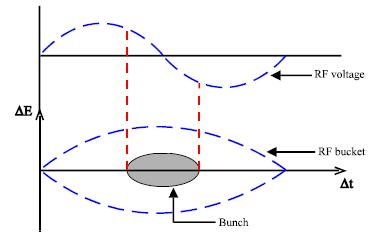
\includegraphics[width=0.3\textwidth]{Chapter2/bunch.png}
	\centering
	\begin{center}
		\caption{The protons are formed into a bunch in the EM wave. This image is taken from \cite{Baird:1017689}}
		\label{Fig:bunch}            
	\end{center}
\end{figure}
\noindent
\\
\\Each LHC beam could have up to 3564 bunches with $\mathcal{O}^{12}$ protons in each bunch for a spacing of 25~ns, but not all of them are filled. For the LHC 2018 operation, the ``filling scheme''  has around 1000-2500 bunches filled, while the remaining ones are left empty (filling scheme most of time is constrained due to technical issues). A series of continuous bunches is called a ``bunch train''. This scheme would then be used to configure the trigger and data acquisition system for the active window of detector operation.
\\  
\\{\bf Collision}
\\
\\The LHC has two beams going in opposite directions with the same configuration (bunch structure, luminosity and energy), and the two beams cross at locations where four detectors are sited: ALICE\cite{alicetdr}, ATLAS\cite{atlastdr}, CMS\cite{cmstdr}, and LHCb\cite{lhcbtdr}. Before stable beams, the two beams pass each other where they are supposed to cross. When both of the beams are ready, the two beams are slightly shifted to target on each other for the collisions .  The crossing angle between the two beams plays an important role in detector performance. It should not be too big, or it would have an impact on physical object reconstruction (see section. \ref{sec:obj rec}) which assumed a zero crossing angle. However, it also should not be too small, or the two beams would interfere with each other. The crossing angle is kept optimized during LHC operation even when the detectors are taking data for physics.
\\
\\When collisions happen, the two crossed bunches usually have more than one pair of interacting protons. In physics, only the most energetic one gets the attention for study, while the other ones are the background contribution called "pile-up events". For ATLAS 2018 operation, the pile-up events could number up to 70 per bunch crossing, and it is now a major challenge of analyses to suppress this type of background.
\\
\\The collisions are then taken as ``instant luminosity'' for the measurement on the amount of data:
\begin{equation}
\mathcal{L}_{inst} = \frac{N}{t\times S^{eff}}
\end{equation}
with N as the number of collisions and $S^{eff}$ as the effect area of the LHC beams for the collisions \footnote{$S^{eff}=4\times\pi\times(1.6\times 10^{-5})^2[m^2]$ for the LHC configuration.}. Then, the total collected data with time is presented as:
\begin{equation}
\mathcal{L} = \int \mathcal{L}_{inst}dt
\end{equation} 
\section{ATLAS Detector}
The ATLAS detector (A Toroidal LHC ApparatuS) \cite{Airapetian:391176} is designed as a general purpose detector\footnote{The other general purpose detector hosted by LHC is Compact Muon Solenoid (CMS). The discovery of any new physics shall be verified by both the ATLAS and CMS collaborations} aiming for most high energy physics physics topics in the energy scale LHC provides like SM precision measurement and searches for new physics.

The ATLAS detector is in a cylinder shape with dimensions of 44m in length and 25m in diameter. Its inner structure is like an onion with multiple layers from the inner most tracking system to the outer part of muon spectrometer functioning to capture different physical objects which will be explained in the following. In the purpose of measuring the particle mass and charge, ATLAS also has two magnetic systems (a solenoid and a toroid) located outside inner tracking system and muon spectrometer. The diagram of the whole ATLAS detector is shown in Fig. \ref{Fig:ATLAS} with the two minimum bias trigger scintillators (MBTS) at both ends.

\begin{figure}[!h]                
	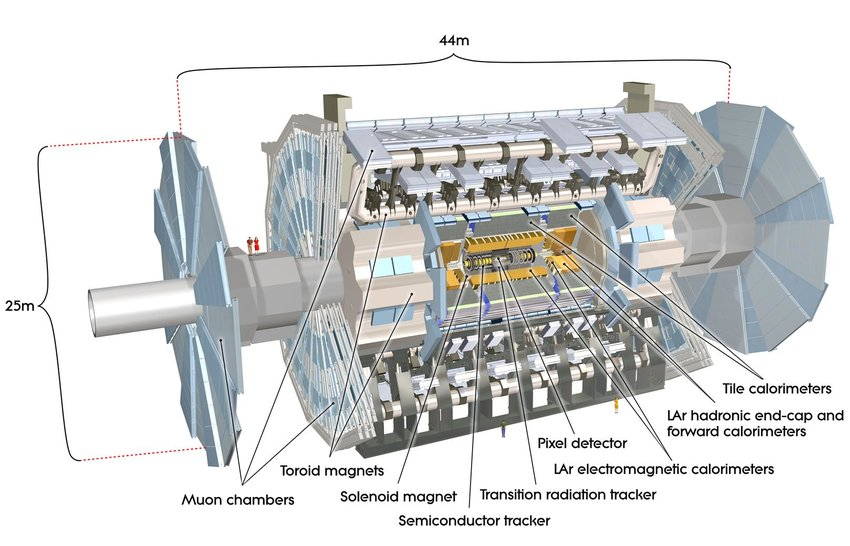
\includegraphics[width=0.8\textwidth]{Chapter2/ATLAS.jpg}
	\centering
	\begin{center}
		\caption{The diagram of the ATLAS detector taken from \cite{Collaboration_2008}}
		\label{Fig:ATLAS}            
	\end{center}
\end{figure}

To define the object positions inside this massive and complicated giant, the coordinate is applied as shown in Fig. \ref{Fig:coordinate}. The x-axis is defined pointing to the centre of the LHC, while the z-axis is the cylinder axle toward the direction of solenoid magnetic field. Then, the y-axis could be found with the right-hand rule. However, this Cartesian coordinate is not convenient in a cylinder, so, instead, the spherical system ($\theta$:angle related to z-axis, $\phi$:angle related to x-axis) is adopted in terms of physics. To keep the parameters as Lorentz invariance, $\theta$ is interpreted into pseudorapidity, $\eta$:
\begin{equation}
\eta = -\ln{\tan{\frac{\theta}{2}}}
\end{equation}
\begin{figure}[!h]                
	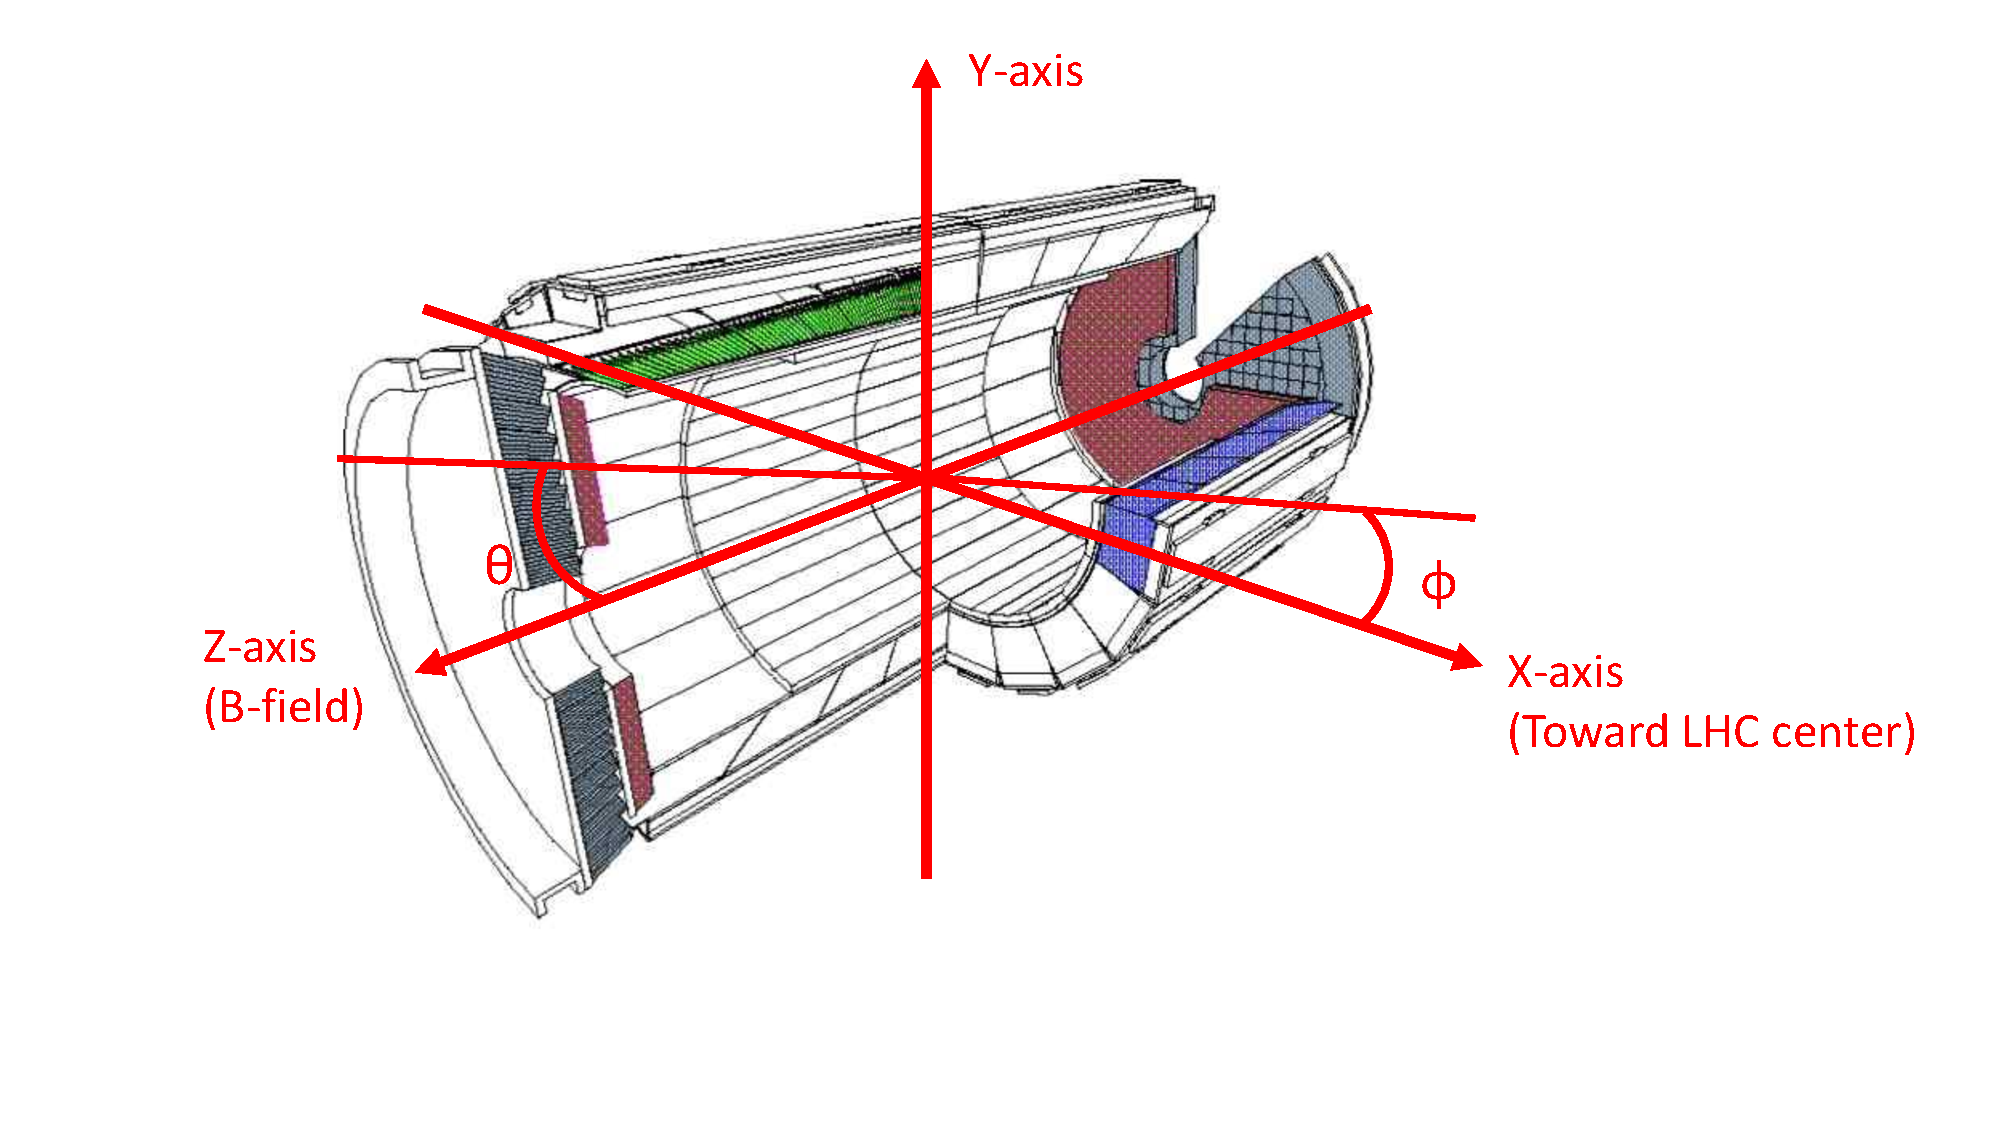
\includegraphics[width=0.95\textwidth]{Chapter2/coordinate}
	\centering
	\begin{center}
		\caption{The coordinate system used in the ATLAS detector}
		\label{Fig:coordinate}            
	\end{center}
\end{figure}
With this definition, the variation of $\eta$ is different from $\theta$, which can be seen in Fig. \ref{Fig:pseudorapidity}. This quantity is important, because the distance between two particles in the detector is defined as:
\begin{equation}
\Delta R= \sqrt{\Delta \eta^{2}+\Delta \phi^{2}}
\end{equation}
For the same $\Delta R$, the separation would be actually larger in the high $\eta$ region especially at $|\eta|>3.2$ (``endcap'' and ``forward'' regions).  
\begin{figure}[!h]                
	
\includegraphics[width=0.4\textwidth]{Chapter2/pseudorapidity.png}
	\centering
	\begin{center}
		\caption{The Psedorapidity varied with $\theta$ from \cite{pseudorapidity_wiki}}
		\label{Fig:pseudorapidity}            
	\end{center}
\end{figure}

\subsection{Inner Detector (ID) \cite{CERN-LHCC-97-016}}
%remember to mention MBTS
The design of a general detector usually consists of two types of system: ``trackers'' and ``calorimeters''. The tracker is used to record the particle trajectories inside the detector with the lowest disturbance on its energy, while calorimeters trap the particles to measure its total energy sum, $E$. 
\\
\\The ATLAS Inner detector is designed as a ``tracker'', so it is used to take the tracks of particles from the collisions. It stands at the inner most part of the detector and spans from 3cm to 108cm in radius with several layers from three subsystems which are pixel, semiconductor tracker (SCT) and transition radiation tracker (TRT) as shown in Fig. \ref{Fig:ID}. 

\begin{figure}[!h]                
	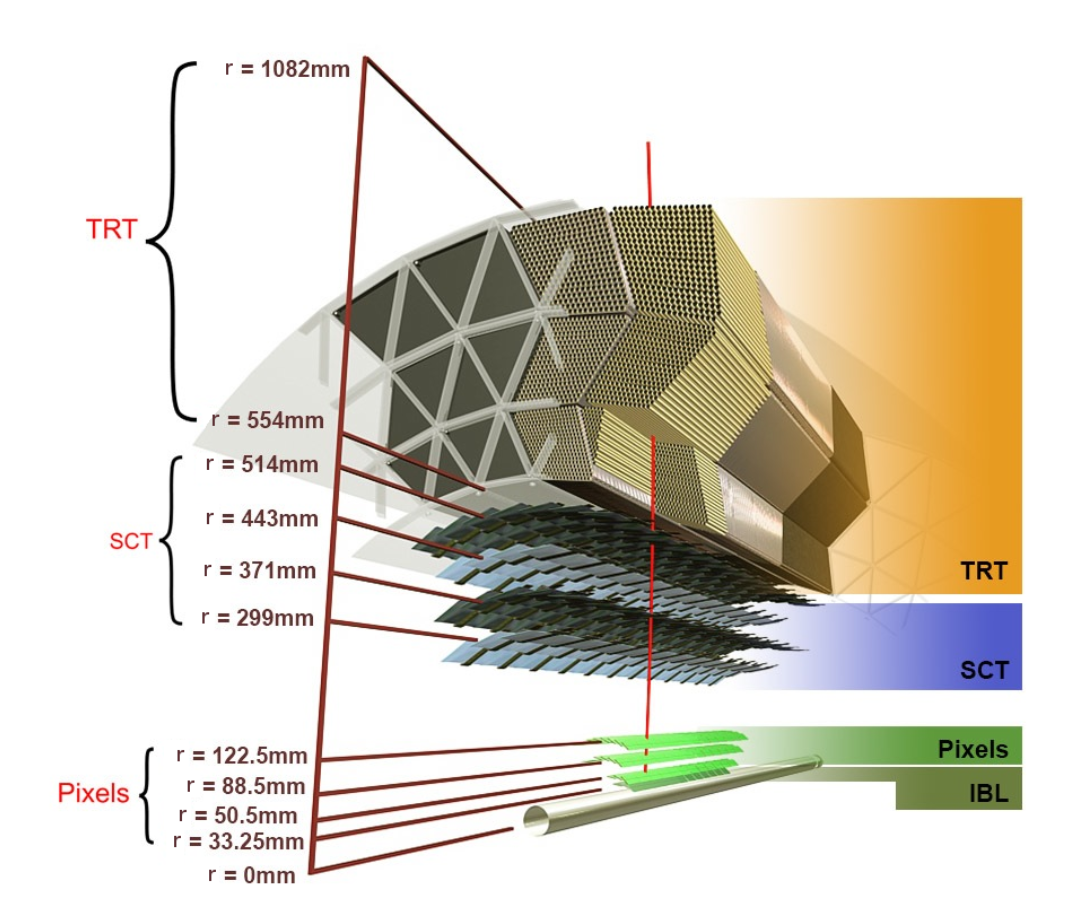
\includegraphics[width=0.7\textwidth]{Chapter2/ID.png}
	\centering
	\begin{center}
		\caption{The diagram for the ATLAS inner detector from \cite{PERF-2015-08}}
		\label{Fig:ID}            
	\end{center}
\end{figure}

Each layer has cells of well-defined granularity. When particles are passing through the inner detector, they leave ``a hit'' per cell on each layer. The tracks are then defined as the link through hits on each layer which are curved lines due to the existence of magnetic field from solenoid, so the curvature of a track could be taken to evaluate the particle momentum and charge. After all tracks are reconstructed, the vertexes are then defined as where the tracks cross. The resolution of transverse momentum, $p_{T}$\footnote{In ATLAS, the activity on transverse plane (i.e. x-y plan) has most of physics interest, because the transverse momentum sum is supposed to be 0, but the case for longitudinal direction isn't}, depends on the particle $p_{T}$ and $\eta$, and it can be presented as:
\begin{equation}
\sigma_{p_{T}} = \sqrt{a^{2}p_{T}^{4}+b^{2}p_{T}^{2}}
\end{equation}
with a and b, the coefficients, depending on track quality and $\eta$. From MC simulation for the track with lease seven hits (a track crossing all layers from pixel and SCT) within $0.25<|\eta|<0.5$, a and b are estimated to be 0.00034 $GeV^{-1}$ and $0.0015$ respectively.
\\
\\{\bf Pixel\cite{Collaboration:2285585}}
\\
\\The pixel detector is the innermost system of ATLAS, and it has the structure of three concentric barrels enclosed by three disks at each end, so all the particles coming out from the collision must pass through all the layers (giving three hits). It provides the best position resolution in the ATLAS detector with a granularity of $50\mu m\times 400\mu m$  for each cell in the $r\Delta \phi \times z$ plane with the coverage of $|\eta|<2.5$ which is used to define the barrel region which has a spatial resolution of $14\mu m\times 115\mu m$
\\
\\In 2014, a new layer of pixel detector called insertable b-layer (IBL) \cite{Miucci_2014} was installed at $3.3cm$ to the beam pipe in addition to the original three layers. Its design is aiming to assist with measurements of short-live particles (like the b quarks whose lifetime is $~10^{-12}s$), so it has an even better granularity of $50\mu m\times 250\mu m$ with extended coverage to $|\eta|<3$. The improved granularity also helps to reduce the uncertainty on impact parameter of collisions.
\\
\\{\bf Semiconductor Tracker}
\\
\\Outside the pixel detector is the semiconductor tracker with three layers in its barrel and nine disks at each end. The sensors are double sided, so when a particle passes through four layers, it leaves totally eight hits in the SCT which form four spacepoints. Different from the pixel detector which has one sensor on each module, the SCT modules have two strip sensors with the width of $80\mu m$ which cross at  an angle of $40mrad$ giving a spatial resolution of $17\mu m \times 580 \mu m$ in the $r\Delta \phi \times \Delta z$ plane. 
\\
\\{\bf Transition Radiation Tracker}
\\
\\The last part of the inner detector is the TRT detector. It doesn't have a multiple layer structure as the pixel or SCT detectors but just a single thick layer stacked of straw drift tubes. Each straw has the diameter of 4mm (with the drift time correction, the spatial resolution from each measurement is $130\mu m$) and is filled with the gas mixture of $Xe$, $CO_{2}$ and $O_{2}$. The gas mixture is used to optimize the absorption of transition radiation. (Due to the gas leaking problem found in the ATLAS operation from 2009 to 2012 \cite{Mindur:2139567}, part of the gas was replaced by cheaper $Ar$-based gas.) When a charge particle passes through the gas, the emitted photon (transition radiation) induces a ``charge avalanche''. This detector allows to the distinguish between electrons and charged pions (because light particles emit more transition radiation).
\\
\\{\bf Magnets}
\\
\\ The ATLAS detector has two superconducting magnet systems different from the CMS experiment with only one solenoid magnet. The inner one is the solenoid magnet located between the TRT detector and the calorimeter, while the toroid magnet is situated in the muon spectrometer system. The advantage of this design is to have the light material (solenoid) inside the detector for transparency, and the toroid still provides the magnetic field to further improve the resolution of momentum measurement\cite{magnets}.  
\\
\\The solenoid magnet is with a diameter of $2.56m$ and length of $5.8m$.  The magnetic field inside the solenoid is almost uniform of 2T along the z-axis as shown in Fig.~\ref{Fig:bfield} to give the momentum and charge measurement in the inner detector. 
\begin{figure}[!h]                
	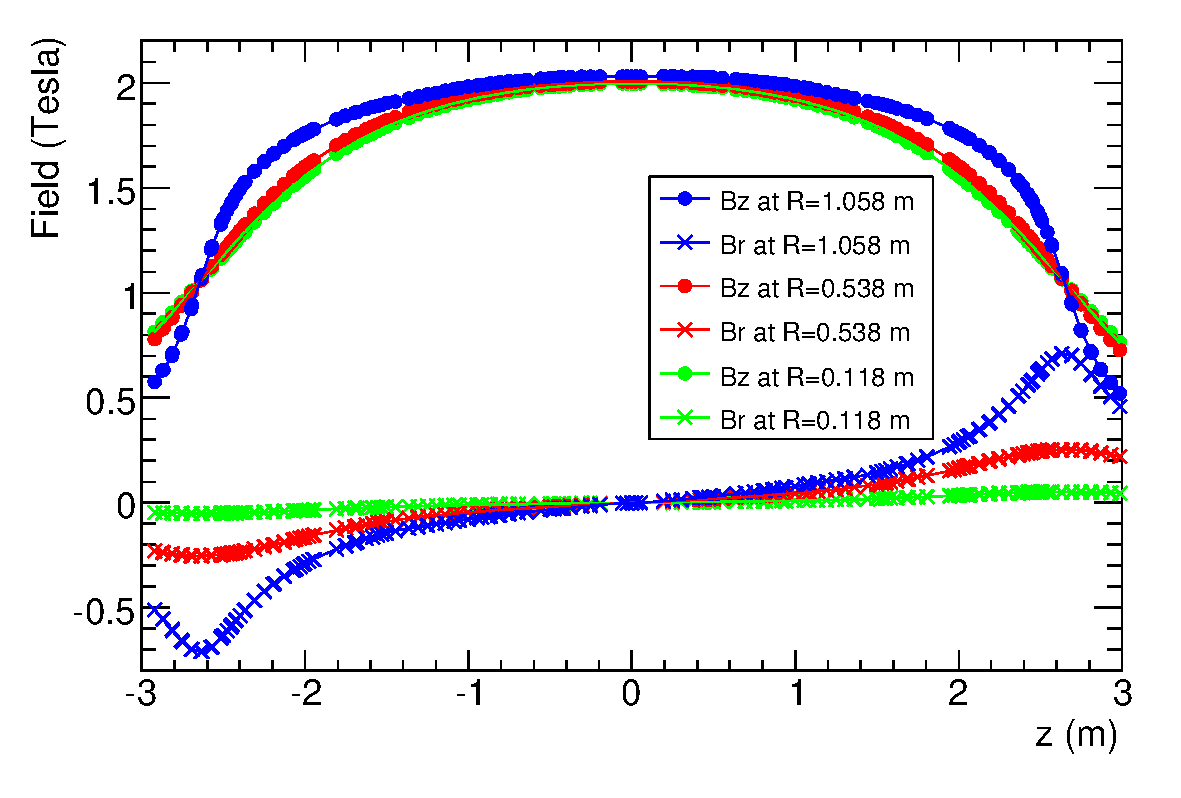
\includegraphics[width=0.6\textwidth]{Chapter2/bfield}
	\centering
	\begin{center}
		\caption{The magnetic field inside the solenoid taken from \cite{Aleksa_2008}}
		\label{Fig:bfield}            
	\end{center}
\end{figure}
\\
\\The toroid magent is composed of the barrel and endcap toroids, and both of them have eight coils providing the magnetic field of 4T in the muon spectrometer. The toroid magnet has the advantage that the particle trajectories in the transverse plane are always perpendicular to the magnetic field, so the momentum measurement is simplified. The toroid magnet is for the measurement of muon momentum in the muon spectrometer. 
\subsection{Calorimeter}
Outside the inner detector is the calorimeter, an energy sampling system. In the ATLAS analyses, there is the need to distinguish the fundamental particles with their energy, so two systems of calorimeters are applied to trap particles with different mass: the electromagnetic calorimeter (ECAL) for electrons and photons as well as the hadronic calorimeter (HCAL) for the hadronic particles. Both ECAL and HCAL have the coverage up to $|\eta|<4.9$. For the range of $|\eta|<2.5$ in the barrel region, two types of calorimeter, the liquid argon (LAr) and tile detectors, are used for the ECAL and HCAL, while in the endcap and forward regions is only the LAr detector. To fit into the cylinder shape of the ATLAS detector, the calorimeters are accordion-shaped from the cross section side. The full diagram of the calorimeter system is presented in Fig. \ref{Fig:calorimeter}. 
\begin{figure}[!h]                %
	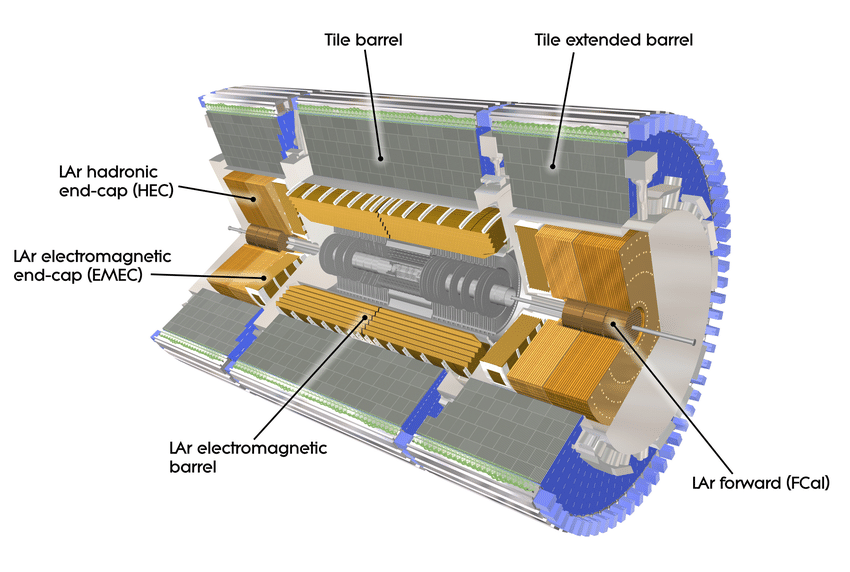
\includegraphics[width=0.85\textwidth]{Chapter2/calorimeter}
	\centering
	\begin{center}
		\caption{The calorimeter system of the ATLAS detector from \cite{Aad:2008zzm}}
		\label{Fig:calorimeter}            
	\end{center}
\end{figure}
The energy resolution for the calorimeter could be presented as:
\begin{equation}
\sigma (E)=\sqrt{a^{2}+b^{2}E+c^{2}E^{2}}
\end{equation}
where a, b, and c are the coefficients. The first term is due to the electronic noise (constant), and the second term is from the shower development of the Poisson fluctuation for the number of shower particles, while the third terms is for the calorimeter non-uniformities (linear to the true shower energy). From the test beam data, the coefficients for the ECAL are $0.4GeV$, $0.1\sqrt{GeV}$ and $0.0017$ for a, b, and c. In terms of the HCAL, the resolution is a bit worse with $1.6GeV$, $0.52\sqrt{GeV}$ and $0.03$. The degraded resolution is due to the intrinsic property of the measurement on hadronic objects which have the energy contribution from neutrinos or binding energy between hadrons. 
\\
\\{\bf Electromagnetic Calorimeter}
\\
\\In ATLAS, the ECAL is made up of the LAr detector\cite{ATLAS:1996ab} each module of which has one absorber and one electrode, and liquid argon is the medium between them. When a particle hits the absorber, it induces the shower, and the shower electrons ionize liquid argon atoms. All the electrons from the interactions would then be collected by the electrodes. The measured current is used to estimate the energy of the incoming particle. The process could be seen in Fig. \ref{Fig:larshower}.\\
\begin{figure}[!h]                
	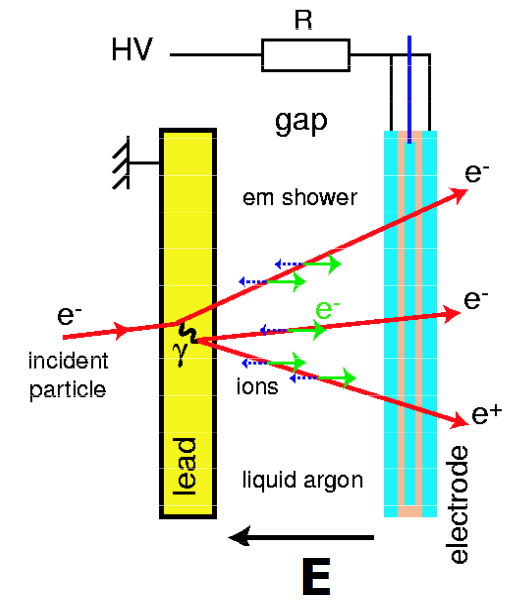
\includegraphics[width=0.35\textwidth]{Chapter2/LArshower}
	\centering
	\begin{center}
		\caption{The interaction between an electron and the LAr calorimeter taken from \cite{LArwork}}
		\label{Fig:larshower}            
	\end{center}
\end{figure}
\\The barrel LAr detector has three sampling layers with different depth and granularity. An extra presampler (layer 0) was added for $|\eta|<1.8$ which has no absorber but only a thin LAr sampler to recognize photons from $\pi^{0}$ decays. The best granularity is at the strip layer (layer 1) for $0.0031\times ~0.1$ ($\Delta \eta \times \Delta \phi$) \footnote{the granularity for $\Delta \phi$ is a approximation, as it has to complete a circle of an irrational number.}, while the last layer is coarse for $0.05 \times ~0.025$ in terms of $\Delta \eta \times \Delta \phi$. For the energy absorption, the depth is what matters most. The full depth of the three sampling layers could correspond to $\sim$22 lead radiation lengths ($X_{0}$) or 2 nuclear interaction length ($2\lambda$).\footnote{the radiation length is defined by the electron energy loss, while the nuclear interaction length is defined by the hadronic object energy loss.} When the ECAL is extended to the region of $2.5<|\eta|<3.2$, only the last two layers would remain, but they still have $18X_{0}$ in total.
\\
\\{\bf Hadronic Calorimeter}
\\
\\Behind the LAr detector is the three-layer tile detector covering $|\eta|<1.7$ with a crack\footnote{The crack is for the supporting structure and output cables} at $1.37<|\eta|<1.52$. It operates in the similar way to the LAr detector, but the absorber material is scintillator. Each sensor of this system is coarser as compared to LAr ones with $0.1 \times ~0.1$ ($\Delta \eta \times \Delta \phi$) for the first two layer and $0.1 \times 0.2$ at the third layer. With the need for the absorption of hadronic objects, it has $8 \lambda$ in the depth for all three layers.
\\
\\In the endcap region ($1.7<|\eta|<3.1$), another type of LAr detector with copper absorber is used as the HCAL. It contains four layers which have the same granularity for $0.1 \times 0.1$ ($\Delta \eta \times \Delta \phi$) in the region, $1.7<|\eta|<2.5$, and $0.2 \times 0.2$ in $2.5<|\eta|<3.1$
\\
\\{\bf Forward Calorimeter \cite{Artamonov_2008}}
\\
\\In contract to the inner detector, the calorimeter should capture as many particles as possible, so the missing energy carried by invisible particles could be estimated by energy conservation within the detector. Therefore, a forward detector is installed at $3.1<|\eta|<4.9$, and it has the best rapidity coverage among the ATLAS subsystems. 
\\
\\The type of detector used here is the third type of LAr detector with tungsten absorber. It has three layers with the first one for ECAL and the last two for HCAL with the same depth of $10\lambda$ (ECAL+HCAL).  
\subsection{Muon Spectrometer\cite{MS_all}}
The outermost detector is the muon spectrometer (MS). Because of their large mass and lack of strong interactions, only muons could travel through the calorimeter and leave signatures here. The muon spectrometer is composed of four types of detectors: thin gap chamber (TGC), resistive plate chamber (RPC), monitored drift tubes (MDT), and cathode strip chamber (CSC) with the toroid magnet system.  
\\
\\In this subsystem, the MDT and CSC are the two detectors providing the tracking measurement with a three-layer structure. In the coverage of $|\eta|<2.0$, all the three layers are composed of the MDT detector, while the innermost layer is replaced by the CSC detector in the extent of $2.0<|\eta|<2.7$ for the effectiveness of high particle density environment. The overall tracking measurement has the spatial resolution of $35 \mu m$
\\
\\However, the precise tracking measurement of the MDT and CSC comes with the cost of a poor temporal resolution, so the RPC ($|\eta|<1.05$) and TGC (($1.05<|\eta|<2.7$)) are interspersed in tracking layers with the time resolution of $25ns$ (with the consideration of uncertainty from cosmic muons). With the fast response, they are part of the ATLAS hardware trigger system. The overall detector performance is summarised in Tab. \ref{Tab:ms}.

\begin{table}[h]
	\caption{Muon Spectrometer Subdetector Performance}
	\renewcommand{\arraystretch}{1.3}
	\centering
	\begin{tabular}{l | c | c | c | c | c }
		\hline
		\hline
		{\bf Type}     &{\bf Function} &{\bf coverage}    &{\bf z/R resolution}  &{\bf $r \Delta \phi$ resolution}&{\bf time resolution}\\
		\hline
		MDT            &tracking       &$|\eta|<2.7$      &$35\mu m$(z)          &N/A                             &N/A            \\
		\hline
		CSC            &tracking       &$2.0<|\eta|<2.7$  &$40\mu m$(R)          &$5mm$                           &$7ns$          \\
		\hline
		RPC            &trigger        &$|\eta|<1.05$     &$10mm$(z)             &$10mm$                          &$1.5ns$         \\
		\hline
		TGC            &trigger        &$1.05<|\eta|<2.7$ &$2-6mm$(R)            &$3-7mm$                         &$4ns$           \\
		\hline
	\end{tabular}
	\label{Tab:ms}
\end{table}

\subsection{Trigger System}
The LHC has the collision rate at $~40MHz$, which leads to the data rate over $60TB$ per second. However, most of the events have no physical interest, because they are just the products of low energy hadronic interactions. Therefore, the trigger system is developed to select events which are going to the storage.
\\
\\For data-taking, the ATLAS trigger system has a two-level structure: the hardware-based L1 trigger (L1) and the software-based high level trigger (HLT). The L1 system is based on the front-end electronics with the logic of selection written by FGPA. Its feature is to make a fast reconstruction of physical objects with a degraded resolution, and it delivers the events at the rate of $100kHz$ ($100k$ events per second). As the detector signatures from the calorimeter and MS are irrelevant to each other, they have their independent L1 trigger systems: L1Calo and L1MU. After the physical objects objects are reconstructed in the two systems, they are then sent to the L1Topo system for the estimation on the topological relation between them. The final trigger decision would eventually be made at the central trigger processor (CTP) by whether a event contains the objects with energy or topological parameters fulfilling the defined criteria. Afterwards, those objects are further processed with a more complicated reconstruction algorithm to give the HLT trigger decision, and the output event rate is reduced to $\sim 1kHz$. The full trigger system is shown in Fig. \ref{Fig:trigger}.

\begin{figure}[!h]                
	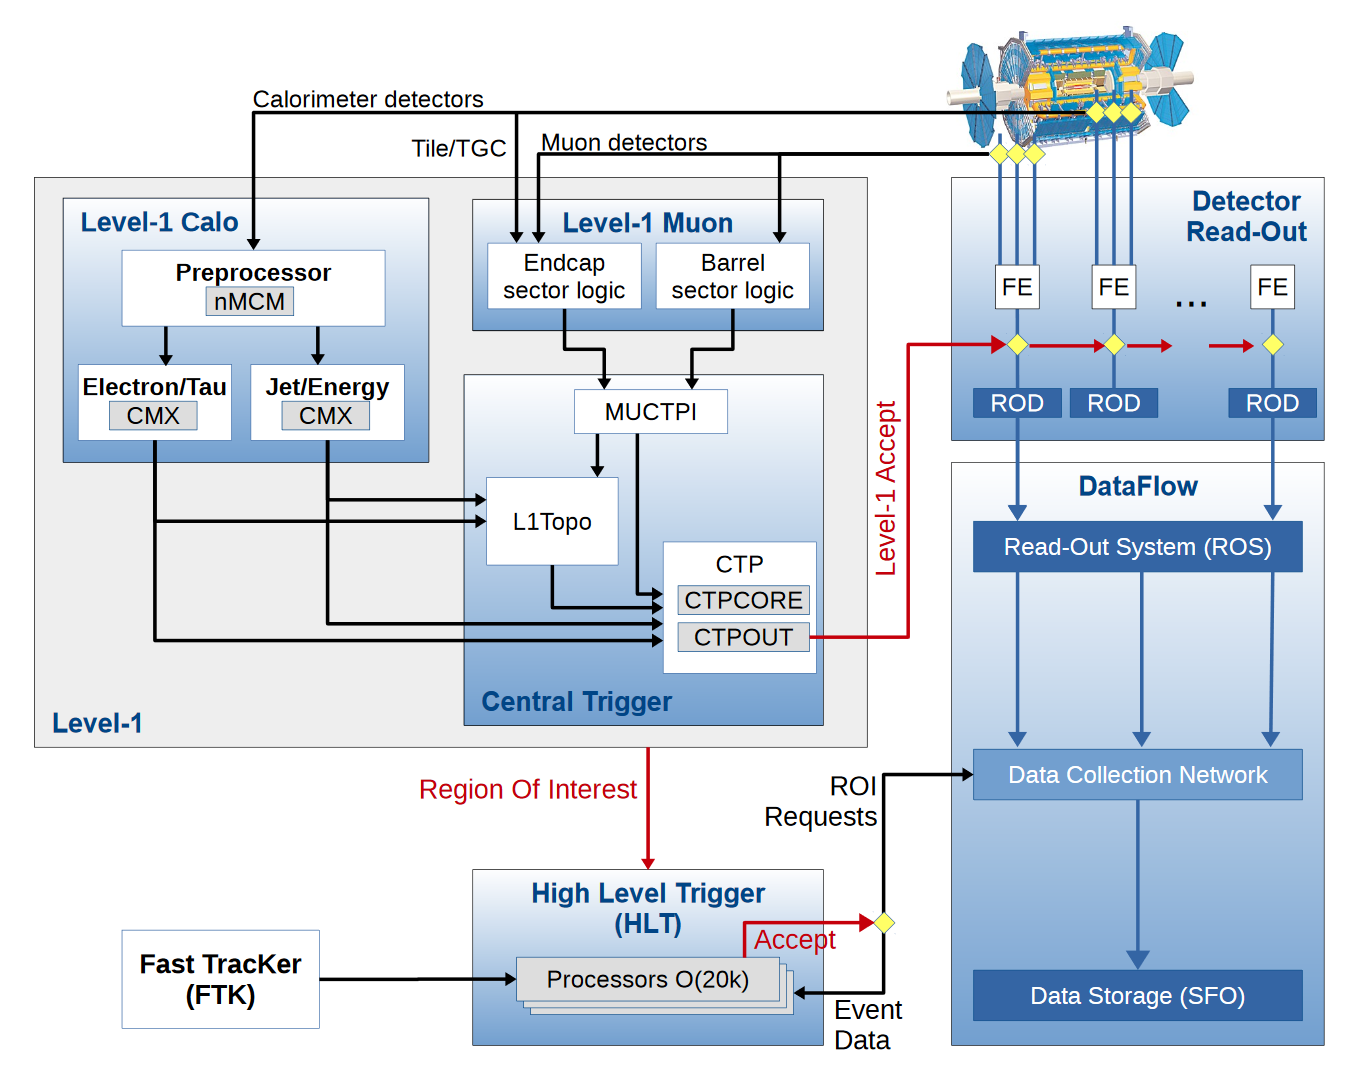
\includegraphics[width=0.8\textwidth]{Chapter2/Trigger.png}
	\centering
	\begin{center}
		\caption{The ATLAS trigger system from \cite{trigger_str}}
		\label{Fig:trigger}            
	\end{center}
\end{figure}
\noindent
\\{\bf L1Calo}
\\
\\When the detector signatures are received from the calorimeter, they are firstly sent to the readout buffer and the L1Calo sysetm. The first component in the L1Calo electronic system is the preprocessor where the signatures are processed into trigger towers with degraded granularity and sent to the processors for physical object reconstruction. Electrons, photons and taus are reconstructed with the trigger tower of $0.1 \times 0.1 (\Delta \eta \times \Delta \phi)$ in the cluster processor (CP), while hadronic objects and missing transverse energy ($E_{T}^{missing}$)\footnote{As the protons only have the longitudinal momentum, the transverse direction momentum should be conserved after collisions} are processed in jet energy processor (JEP) with a coarser granularity of $0.2\times 0.2$.
\\
\\{\bf L1MU}
\\
\\The L1MU system is taking the data from the RPC and CSC which have great time resolution as fast as $1.5\mu s$ but with a poor spatial resolution. It receives signatures from the MS barrel and endcaps where they are processed respectively. To further suppress the rate contributed by fake muons, the L1 muons are reconstructed with consistent hits from the TGC at the endcap ($1.05<|\eta|<2.7$). 
\\
\\{\bf HLT}
\\
\\When the trigger decision was made to accept an event, the regions of interest (ROI) with the original detector granularity are passed to the HLT. The HLT is runs on a CPU farm where the more complicated algorithms are deployed to reconstruct the physical objects. Due to the finer granularity and longer latency, it provides better precision on both energy and spatial resolution. When the events fulfil the HLT criteria, they are then sent to storage. 
\\
\\{\bf ATLAS Trigger Menu}
\\
\\An ATLAS trigger is generally a trigger chain composed of L1 and HLT items. When an HLT trigger is fired, there is always a corresponding L1 trigger decision. For example, HLT electron trigger shall only be passed when a L1 electron trigger is also fired:
\begin{equation}
L1\_e24 \rightarrow HLT\_e26\_lhtight\_nod0\_ivarloose
\end{equation}
where the numbers are the trigger thresholds in the unit of $GeV$, while the $lhtight$ and $ivarloose$ are to define the electron quality with the calorimeter activities in the surrounding region of this electron (see more details in Sec. \ref{sec:obj rec}) . The threshold of triggers might not be kept the same during the operation at periods. Because the LHC keeps pushing its performance on instantaneous luminosity, the energy contribution from pile-up events enhances the trigger rate above the allowed bandwidth for data storage. To make better suppression on the trigger rate, the thresholds are therefore raised during some operation periods. 
\\
\\The defined triggers would then be made into ``streams'' where the events are categorized for different purposes. Physics analyses shall use the triggers contained in the ``$physics\_main$'' stream, and there are also the dedicated streams composed of ``prescaled'' triggers for hardware calibrations. Those calibration triggers usually have lower thresholds in contract with the ones in $physics\_main$. A random sampling is applied to only pick a fraction of events passing those triggers, which makes them unsuitable for physics analysis. The total allowed output rate from all streams is $5kHz$ with $1kHz$ for $physics\_main$. 

\subsection{Run 2 Operation Overview}
For the ATLAS operation from 2015 to 2018 which is called Run 2 (with respect to Run 1 from 2009 to 2013), the average data recording efficiency is around $95\%$ with respect to LHC delivery efficiency. From the measurement with the Lminosity  Cherenkov  Integrating  Detector (LUCID, one of the forward detectors of the ATLAS)\cite{Bruschi:2025000, ATLAS:2019pzw}, the integrated luminosity is $\sim~36fb^{-1}$ for 2015 and 2016, $\sim46~fb^{-1}$ for 2017 and $\sim63~fb^{-1}$ for 2018 which gives the total data of $140 fb^{-1}$. The performance from 2011 to 2018 is summarized in Fig. \ref{Fig:recefficiency}
\begin{figure}[!h]                
	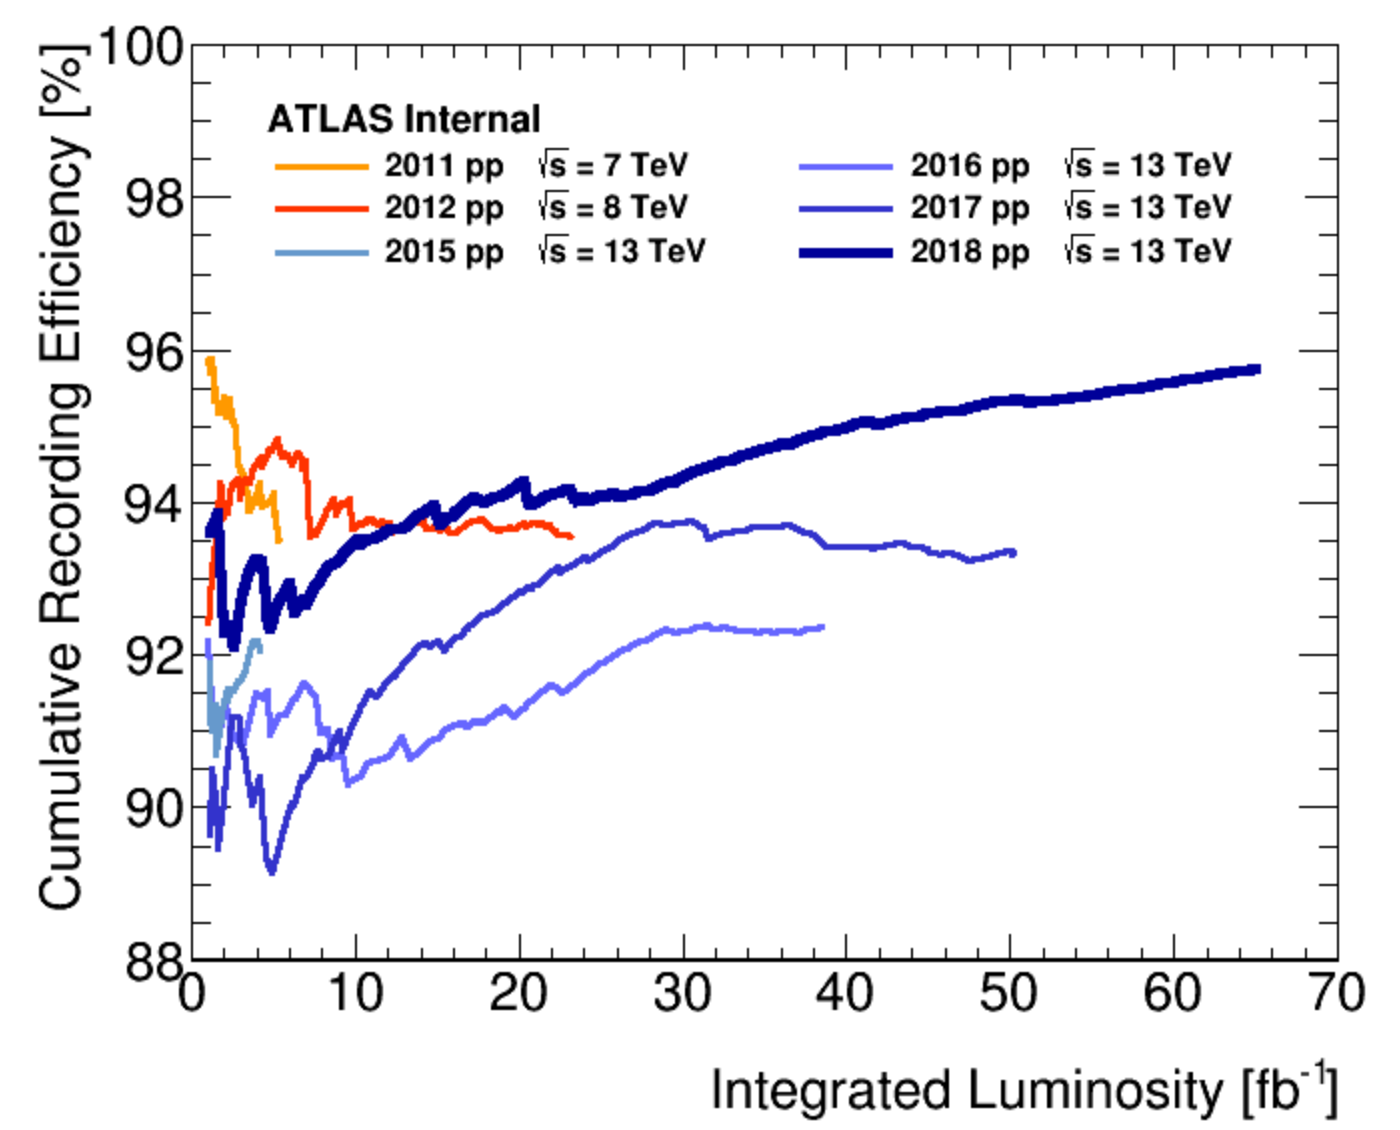
\includegraphics[width=0.6\textwidth]{Chapter2/recefficiency.png}
	\centering
	\begin{center}
		\caption{The ATLAS recording efficiency and luminosity \cite{Pontecorvo:2638061}}
		\label{Fig:recefficiency}            
	\end{center}
\end{figure}
\section{Object Reconstruction}
\label{sec:obj rec}
When the events are passed into the permanent storage, they are still in the format of raw data which contains only the information of hits (the spacepoints from the inner detector and muon spectrometer) and calorimeter energy towers (the energy deposited in the calorimeter cells). They need to go though the full reconstruction (offline reconstruction) to be interpreted into the objects with physical meanings as the SM particles like electrons or muons. The reconstruction will be based on the principles of interactions between detectors and particles: 
\\
\\1) Only charged particles leave tracks in the inner detector
\\
\\2) The charged particles shall deposit energy in the ECAL, and the light ones are stopped here.
\\
\\3) All the particles except for muons are supposed to be stopped in or before the HCAL.
\\
\\4) Only muons could reach the muon spectrometer. 
\\
\\After the reconstruction of all subjects, a further correction on energy scale (the peak of the energy pulse shape) is applied on both data and simulation samples to take in  the effect of energy loss from the radiation, the contamination from other objects, or the detector effect (like dark current, hot noise, or material inhomogeneities). The final procedure is to remove the overlapped objects by the priority defined by the analyses. 
\\
\\{\bf Primary Vertex $\&$ Tracks \cite{Aaboud:2017all}}
\\
\\A pattern recognition is performed in the SCT to find the helical trajectories with at least 3 spacepoints and $p_{T}>500MeV$ which are taken as the track seeds. A Kalman Filter algorithm is then performed to extend the track seeds to the pixel layers. To resolve the reconstruction ambiguity, a tracking score system is taken to reject the shared spacepoints or fake tracks. When a track is reconstructed with more hits and less ``holes'' (missing hits in some layers), it is given a higher score. The final tracks shall all have at least seven hits (three spacepoints from SCT and four hits from pixel). To complete the track reconstruction, the projection route from the outermost SCT spacepoint of a track passes through TRT, and the drift tubes within $10mm$ from the route are integrated into the track. Afterwards, one addition track reconstruction (outside-in) from TRT is performed to recover the tracks from the late decay or photon conversion. The unused TRT segments are then rematched to the SCT and pixel hit remanent.   
\\
\\The crossing points of tracks near the LHC pipelines are then assumed to be where the interactions happen, which are called ``vertices''. The vertex associated with the highest $p_{T}^2$ sum is then defined as the primary vertex. All the reconstructed objects should origin from the primary vertex which is verified by $d_{0}$ and $d_z$, the distances between the object and the primary vertex in the x-y plane and the z-axis, or they are taken as ``minimum bias'' background.  
\\
\\{\bf Electrons}
\\
\\Electrons are charged light particles, so they leave tracks in the inner detector and energy clusters in the ECAL. The two types of signature are combined and testified to reconstruct electrons.
\\
\\The first stage of the reconstruction is to build the energy cluster as an electron seed \cite{ATLAS-CONF-2016-024,ATL-LARG-PUB-2008-002}. A window of $3 \times 5$ ECAL layer-2 cells (corresponding to $0.075 \times 0.125$ in $\Delta \eta \times \Delta \phi$) is used to scans through ECAL layer-2 to find the electron seeds. If the transverse energy sum ($E_{T}$) inside the window is above $2.5GeV$, the cells inside this window are selected, and the electron position is defined as the energy weighted $\eta$ and $\phi$ (barycentre) of this window. Then, this window is extended along the $R$-direction to sum over the energy in other layers with the adjusted window size (detailed in ~\cite{}). The cells taken in the cluster are then removed to avoid the duplication into other electrons. With the estimation from $Z\to ee$ simulation sample, this algorithm has the electron reconstruction efficiency of $95\%$ ($>99\%$) for $E_{T}\sim7GeV$ ($E_{T}>15GeV$).
\\
\\The reconstruction of tracks associated to electrons is performed independently from the mentioned reconstruction . A track seed of $p_{T}>1GeV$ is firstly reconstructed with three spacepoints from the SCT layers . Then, based on the pion hypothesis (pion energy loss pattern in the ID materials), it is verified by whether this track seed can be extended to pixel with four hits and matched to a calorimeter cluster. If it fails, the electron hypothesis is applied for the same verification. The hits from both hypotheses are then fitted using ``ATLAS Global $\chi^{2}$ Track Fitter''\cite{Cornelissen:2008zza} into tracks, and the tracks failing the pion track hypothesis are then tested again with electron hypothesis. The tracks passing the electron hypothesis are then taken as potential electron tracks. This algorithm is also integrated in the standard track reconstruction with the least interference.
\\
\\The track and cluster are then associated with a loose $\Delta R$ matching which considers the electron bremsstrahlung and the number of hits in the inner detector. The matched track-cluster pairs are then refitted with optimised ``Gaussian Sum Filter'' (GSF) \cite{ATLAS-CONF-2012-047} to take non-linear bremsstrahlung into account. 
\\
\\To have further separation between signal-like and background-like electrons, the electron identification is then performed on $Z \rightarrow ee$ (signal) and dijet (background) MC samples. It is a multi-variable analysis (MVA) based on the likelihood discriminant defined as:
\\
\begin{equation}
d_{\mathcal{L}}=\frac{\mathcal{L}_{S}}{\mathcal{L}_{S}+\mathcal{L}_{B}}    
\quad \text{ and } \quad
\mathcal{L}_{S(B)}(\vec{x})=\prod_{i = 1}^{n}P^{i}_{S(b)}(x^{i})
\end{equation}
where $P^{i}_{S(b)}(x^{i})$ is the probability density function for a specific input variable $x^{i}$, and $\vec{x}$ is the vector formed by them in the likelihood phase space of all input variables (all the input variables could be found in \cite{}). Three working points are therefore defined by $d_{\mathcal{L}}$: $Tight$, $Medium$ and $Loose$\footnote{$Tight$ selected electrons are the subset of $Medium$, and $Medium$ is the subset of $Loose$}. The signal efficiency from this selection process is as a function of electron $E_{T}$, and the plateau of efficiency could be reached at $E_{T}~70GeV$ for $~97\%$ ($~95\%$) [$91\%$] on $Loose$ ($Medium$) [$Tight$] working point. 
\\
\\In addition to the reconstruction quality, the electrons are also required to be ``isolated'' from all the other tracker and calorimeter signatures, because of the concern that the nearby detector activities might affect the electron measurement. The isolation is defined in two ways: 
\begin{itemize}
	\item the calorimeter isolation ($Iso^{E_{T}}$): it is defined as the cluster $E_{T}$ sum within a cone with $R=0.2(0.3)$ centred at the reconstructed electron inside which a central cluster subset in a rectangle of $0.125 \times 0.175$ ($\Delta \eta \times \Delta \phi$) is subtracted.
	\item the track isolation ($Iso^{p_{T}}$): it is defined as the $p_{T}$ sum of tracks from primary vertext within a cone of $R=min(0.2(0.3), 10GeV/E^{e}_{T})$ centred at the electron but without the electron associated tracks.  
\end{itemize}
The isolation discriminant is then applied as $Iso^{E_{T}}/E_{T}$ or $Iso^{p_T}/p_{T}$. The recommendation working points on the discriminant are given as a function of $E^{e}_{T}$ or fixed cut which are summarised with the muon isolation working points in Tab. \ref{Tab:iso}. 
\\
\\{\bf Muons \cite{Herde:2059849}}
\\
\\Muons are heavy enough to travel through the calorimeter and reach the MS, but the reconstruction is mainly based on the tracks in the inner detector and the MS. 
\\
\\The MS track segments are firstly built from the hits within each MS module, but the reconstruction coordinates are different in each subsystem: the MDT reconstruction is on the coordinate of the toroid magnetic bending plane, while the RPC and TCG have the coordinate orthogonal to it, and the CSC is only using the detector $\eta$-$\phi$ coordinate. A loose criteria is applied in the segment building algorithm to verify the compatibility to a full track. Then, the segments in the middle layer of the MS are taken as the track seed and extended to the inner and outer layers. If two segments could be fitted with enough hits by matching from their relative position and angle, they are integrated into the same track. The exception is in the transition region between the barrel and endcap, and a standalone and good-quality segment could be kept as a single track.  
\\
\\An overlap removal is afterwards applied to remove the shared hits in the tracks with poor fitting quality, but they could still be kept only if the fitting criterion is fulfilled. Two tracks could share maximally two hits in the inner two layers and have no same hit in the outer layer for the concern of close-by muons. 
\\
\\The hits along the tracks are then taken into the global $\chi^{2}$ fitting. The hits with great deviation from the fitted MS trajectory are removed, and the fit is applied again to derive the new track. If there are hits not included in the track but within the allowed deviation from the track, they are also taken into the track, and the fitting is repeated. 
\\
\\The final MS tracks are taken as the seed to match to the inner detector tracks to reconstruct the combined muons. A further global fitting is conducted to extrapolate the muons with the flexibility to add in or remove the MS hits to improve the fitting quality with the ID tracks. The primary algorithm in the fitting is performed outside-in from the MS to the inner detector, and a complementary algorithm of inside-out is also applied to guarantee the robustness of the reconstruction. For the muons outside of the inner detector coverage ($2.5<|\eta|<2.7$), they can be reconstructed from only MS tracks, but the criteria are more stringent. 
\\
\\Similar to electrons, muons also have the identification procedure with three parameters: $q/p$ significance (the ratio of charge and momentum measured in the ID and MS over the quadrature sum of their uncertainty), $\rho'$ (the ratio of momentum difference between the ID and MS measurements over the combined measurement) and the normalised combined track fit, $\chi^2$. The working points for the muons identification have the definition individually as below:
\begin{itemize}
	\item $Medium$ muons: they are defined within the range of $0.1<|\eta|<2.5$ with at least two layers of $\geq 3$ hits. If it is within the range, $0.1<|\eta|$, it is allowed to have hits in only one layer, but there shall be no hole in the MS track reconstruction. As the muons go beyond the coverage of the inner detector (i.e. $2.5<|\eta|<2.7$), they shall have the MS tracks reconstructed from all three layers. An extra requirement of $q/g$ significance above seven is also applied on this muon quality. 
	\item $Loose$ muons: those muons are defined with the most loose requirement. They are generally $Medium$ muons, but the selection is loosen for the range of $|\eta|<0.1$ due to the missing coverage of the MS (where a gap is present for the service of the ID and calorimeter). When an ID track is found within this range and matched to a calorimeter cluster which is identified as a deposit by ``minimum-ionization'' particles, they are also accepted as loose muons to recover the reconstruction efficiency. 
	\item $Tight$ muons: all of them must have the tracks reconstructed from two layers in the MS (either MDT or CSC) with $Medium$ muon hit selection. To enhance the purity of muons, a further requirement on the ID to MS track fitting is also added into the selection for $\chi^2<8$. An addition two-dimension cut on $q/g$ significance and $\rho'$ is also applied to improve the background rejection for muons with $p_{T}<20GeV$.
\end{itemize}
For the muon isolation, the definition is similar to the electron ones, but they have different working points. The recommended working points for electrons and muons are shown in tab. \ref{Tab:iso}.

\begin{table}[h]
	\caption{Electron/Muon Isolation Working Points}
	\renewcommand{\arraystretch}{1.5}
	\centering
	\begin{adjustbox}{center}
		\begin{tabular}{|c | c | c | c | c |}
			\hline
			\hline
			{\bf Working Point} &{\bf Object} &{\bf Calo Iso}                   &{\bf Track Iso}  &{Combined Iso} \\
			\hline
			LoseeTrackOnly      &all leptons  &-                                      &$99\%$                 &$99\%$               \\
			\hline
			Loose               &all leptons  &\multicolumn{2}{|c|}{$99\%$}                                   &$99\%$               \\
			\hline
			Gradient            &all leptons  &\multicolumn{2}{|c|}{$\epsilon=(0.1143*p_{T}[GeV]+92.14)\%$}   & \shortstack{\footnotesize{$\epsilon(25GeV)=90\%$} \\  \footnotesize{$\epsilon(60GeV)=99\%$}}\\       
			\hline
			GradientLoose       &all leptons  &\multicolumn{2}{|c|}{$\epsilon=(0.057*p_{T}[GeV]+95.57)\%$}   & \shortstack{\footnotesize{$\epsilon(25GeV)=95\%$} \\  \footnotesize{$\epsilon(60GeV)=99\%$}}\\
			\hline
			FixedCutTight       &Electrons  &\footnotesize{topoetcone20/pT<0.06}                 &\footnotesize{ptvarcone20/pT<0.06}  &-               \\
			\hline
			FixedCutTight       &Muons  &\footnotesize{topoetcone20/pT<0.06}                 &\footnotesize{ptvarcone30/pT<0.06}  &-               \\
			\hline
			\footnotesize{FixedCutTightTrackOnly}      &Electrons     &-                 &\footnotesize{ptvarcone20/pT<0.06}  &-               \\
			\hline
			\footnotesize{FixedCutTightTrackOnly}      &Muons      &-                 & \footnotesize{ptvarcone30/pT<0.06}  &-               \\
			\hline
			FixedCutLoose        &Electrons  & \footnotesize{topoetcone20/pT < 0.2} & \footnotesize{ptvarcone20/pT < 0.15}  & - \\
			\hline
			FixedCutLoose        &Muons  & \footnotesize{topoetcone20/pT < 0.3} & \footnotesize{ptvarcone30/pT < 0.15}  & - \\
			\hline
			\footnotesize{FixedCutHighPtCaloOnly} & Electrons &  \footnotesize{topoetcone20} < 3.5 GeV & - &-\\
			\hline
			\footnotesize{FixedCutHighPtTrackOnly} & Muons &  - &  \footnotesize{ptcone20} < 1.25 GeV  &-\\
			\hline
		\end{tabular}
	\end{adjustbox}
	\label{Tab:iso}
\end{table}
\noindent
{\bf Jets}
\\
\\When quarks or gluons are travelling in the space, they went through the process called ``fragmentation'' or ``hadronization'' for ``color-confinement'' of QCD. This leads to the multiplication of quarks, gluons (i.e. partons) or even leptons and photons, and they eventually form the bound states as hadrons leaving complicated signatures in the detector. One quark from a collision might leave more than one hundred tracks in the inner detector and several clusters in the calorimeter, and jets are defined as the ensemble of those signatures. To properly collect those tracks and calorimeter clusters into the same jets, the reconstruction algorithm is designed to ensure the infrared safety and collinear safety. The infrared safety means that 
the soft radiation from hadronic objects in a jet would not change the jet width or orientation, while the collinear safety indicates that the nearby particles with higher $p_{T}$ in the collinear direction of the splitted parton would not affect the jet reconstruction. To achieve both of the two requirements, the jet reconstruction algorithm\cite{Atkin:2015msa} employs the following two parameters for the jet definition: 
\begin{equation}
d_{ij}=min((p_{t}^{i})^{a},(p_{t}^{j})^{a})\times \frac{R_{ij}^{2}}{R}
\quad \text{ with } \quad
d_{iB}=(p_{t}^{i})^{a}
\end{equation}
where $p_{t}^{i}$ and $p_{t}^{j}$ are $p_{T}$ of $i$th and $j$th entities which could be calorimeter clusters (a patch of energetic cells in the calorimeter), tracks, or the truth particles from the simulation, $R_{ij}$ is the distance between them, and R is the parameter to customize the algorithm for performance (i.e. cone size), while $a$ corresponds to three algorithms which are sensitive to different jet properties. $a=-2$ is for $anti-k_{t}$ algorithm, and it has the advantage for better stability of jet structure during reconstruction with high sensitivity to hard objects and ignorance for the jet substructure as well as pile-up events. $a=0$ and $a=-2$ are used for Cambridge-Aachen algorithm and $k_{t}$ algorithm respectively which are more sensitive to jet substructure but with high dependence on pile-up events and soft objects. When $d_{ij}<d_{iB}$, the $i^{th}$ and $j^{th}$ objects are merged into the same cluster with the position defined as their barycentre. If no new pair could be found meeting this condition, the cluster is then defined as a jet. To make further 
\\
\\For the jets in the ATLAS experiment, $anti-k_{t}$ algorithm is preferred with $R=0.4$ and $R=1.0$ with the inputs objects. $R=1.0$ is for the scenario that two jets are close to each other, and $R=0.4$ could not have the separation power to distinguish each of them. The input entities for jet reconstruction is the ECAL topo clusters in the range of $|\eta|<4.9$, the calorimeter coverage, with energy $2\sigma$ above the quadrature sum of pile-up events and electronic noise, while the seeding cluster to initiate the clustering has higher requirement of $4\sigma$. The hadronic energy deposit from HCAL is added to the ECAL clusters through ``local cell weighting'' (LCW)\cite{Barillari:1112035} which is to calibrate the jet energy scale by the MC simulation and the data from the single particle test beam. The final reconstructed jets are then used in analyses after the selection of ``jet vertex tagger'' (JVT)\cite{ATLAS-CONF-2014-018} to guarantee that they originate from the primary vertex. 
\\
\\{\bf b-Tagging\cite{ATL-PHYS-PUB-2015-022}}
\\
\\b quarks take over the greatest branch ratio of Higgs boson decay, and it is always the decay product of top quarks(BR($t \rightarrow bW$)=$100\%$) which is the major background for most ATLAS analyses. Therefore, how to recognize the jets from b quarks is an important task for physics purposes.
\\
\\Different from the signatures other stable SM particles leave in the detector, b-quarks have a ``pseudo-short'' lifetime, so the jets of b-quarks have a displaced vertex several $mm$ away from the primary vertex. The b-jet identification depends on this property and the b-quark decay chain. The following three algorithms are used:
\begin{itemize}
	\item {\bf Impact Parameter based Algorithms}: given their displaced vertex, b-jet associated tracks should tend to have a greater impact parameter in both transverse and longitudinal directions. The impact parameters are used as inputs for the probability density function of the ratio of possibility of b-quark and light-flavour quark hypotheses, which are then combined into a single log likelihood ratio discriminant (LLR).
	\item {\bf Secondary Vertex Finding Algorithm}: to reconstruct the secondary vertex, the first step is to find the vertices with only two tracks. The tracks from the vertices far from the primary vertex, they are rejected. They might be from long-lived hadron decay (like kaon), photon conversion or hadronic interaction with materials.  The secondary vertex is then reconstructed from the survived tracks with outlier tracks removed
	\item {\bf Decay Chain Multi-Vertex Algorithm}: this algorithm is also called ``jet finder''. Its purpose is to find the full chain of ``$PV \rightarrow b \rightarrow c$''. A Kalman filter is applied to link the vertices to approximate the trajectories of this jet with which the vertices of b- and c-quarks could be resolved even with only one-track link.  
\end{itemize}
\noindent
The output of those algorithms are then given to a multi-variable analysis (MVA) of Boosted Decision Tree for the final discriminant. It is trained with the sample of $t\bar{t}$ which contains b-jets and the background composed of $10\%$ c-jets and $90\%$ other light-flavour jets. The final outcome, BDT score, is then applied as a simple cut to select b-jets, and the suggested working points are shown in tab. \ref{Tab:b-tag}

\begin{table}[h]
	\caption{b-Tagging Working Points}
	\renewcommand{\arraystretch}{1.5}
	\centering
	\begin{adjustbox}{center}
		\begin{tabular}{|c | c | c | c |}
			\hline
			\hline
			{\bf Cut Value}    & {\bf b-jet Efficiency[$\%$]}  & {\bf c-jet Rejetction} & {\bf light-flavour-jet Rejection}\\
			0.4496 & 60 & 21 & 1900 \\
			-0.0436& 70 & 8.1& 440 \\
			-0.4434& 77 & 4.5&  140 \\
			-0.7787& 85 & 2.6&  28 \\
			\hline
		\end{tabular}
	\end{adjustbox}
	\label{Tab:b-tag}
\end{table}		
\noindent
{\bf Missing Transverse Energy (MET)}
\\
\\The design of the ATLAS detector utilizes electromagnetic and hadronic interactions to capture particles. If particles are only involved in weak interactions, they leave no signatures in the detector like neutrinos or some new particles predicted by BSM theories. In this case, the only way to measure their energy is via the momentum conservation. 
\\
\\When two protons collide into each other in the LHC, both of them have no momentum on the transverse plane, so the transverse momentum sum of collision products is supposed to be zero. Therefore, the definition for sum of transverse momentum from invisible particles could be presented as:
\begin{equation}
\vec{E}_{T}^{miss} = \sum_{\text{visible objects}} -\vec{p}_{T}^{i}
\end{equation}
where $E_{T}^{miss}$ is supposed to be called missing transverse momentum, but it is called ``missing transverse energy'' out of historical reason. The explicit form is:
\begin{equation}
\vec{E}_{T}^{miss} = -(\sum \vec{p}_{T}^{e} +\sum \vec{p}_{T}^{\mu} +\sum \vec{p}_{T}^{\gamma} +\sum \vec{p}_{T}^{jet} +\sum \vec{p}_{T}^{\tau}+\sum \vec{p}_{T}^{soft})
\end{equation}
with $p_{T}$ contributed from different objects passing loose selection. Even though tau, $\tau$, and photon, $\gamma$, are not used in the analysis, they are still reconstructed and applied in $\met$ estimation.  The last term is referred to the detector soft signatures which are not used in the reconstruction of any objects. They could be either from tracks (track soft term, TST) or clusters (cluster soft term, CST). The track soft term considers only the remaining tracks from the primary vertex, so it has lower dependence on the pile-up events, while it cannot deal with the contribution from neutral objects which, instead, could be recovered by the CST. In ATLAS Run2 analyses, TST is preferred, because it delivers smaller uncertainty with the high pile-ups. As $E^{T}_{miss}$ is only calculated on the transverse plan, it has no $\eta$ information. 

\section{Simulation}
\label{sec:simulation}
For the two analyses in this thesis, the SM background estimation comes from the Monte Carlo simulation. It is performed in a couple of steps: event generation $\rightarrow$ event overlapping with ``minimum bias'' (MB) events $\rightarrow$  detector response simulation $\rightarrow$ digitization $\rightarrow$ physical object reconstruction $\rightarrow$ physics analysis.
\\
\\Event generation is through the generators designed by theorist with the input of theoretical parameters for the interactions: $pp(\rightarrow X)\rightarrow Y$. $X$ is the medium state particle with short lifetime, and it will eventually decay to Y as the final stable particles leaving signatures in the detector with the kinematic properties assigned by the event generator. The total cross section of the interaction will then be evaluated by this equation\cite{Plehn:2008zs}: 
\begin{equation}
\sigma_{pp\rightarrow Y} = \sum_{a,b} \int dx_{1}dx_{2}f_{a}(x_{1},\mu_{1})f_{b}(x_{2},\mu_{2})\hat{\sigma}_{a,b\rightarrow X}(x_{1},x_{2},\mu_{R})
\end{equation}
with a,b as the flavours for the proton partons (quark or gluon) involved in the interaction, and $x_{1}$ and $x_{2}$ are the momentum fraction of the partons relative to the whole proton, $\hat{\sigma}_{a,b\rightarrow X}$ is the cross-section calculated perturbatively of the process, $a,b\rightarrow X$, and $f_{a}$, $f_{b}$ are the parton distribution function (p.d.f.) for the corresponding parton flavours which give the possibility of the momentum transfer from partons to the output stable particles. $\mu_{1}$, $\mu_{2}$, and $\mu_{R}$ are the factorization factors which decide how the p.d.f. evolves. 
\\
\\For the ATLAS simulation, two processes are simulated in one event: pile-ups, $pp\rightarrow jj$, and hard-scattering, $pp(\rightarrow X)\rightarrow Y$ with $X$ and $Y$ as the particles of interests. Generally, hard-scattering is generated with a specific generator which can give the best accuracy of simulation, and the events are then passed to $PYTHIA8$\cite{Sjostrand:2008vc,Sjostrand:2007gs} for the generation of pile-up events and the hadronizaton of the hadronic objects. 
\\
\\The next step is to simulate the interaction between the particles and the detector. The detector is described by $GEANT4$\cite{Agostinelli:2002hh} with the input parameters like materials and logical volumes. The detector description is then stored in the ATLAS Geometry database which has low flexibility to change the content, while an additional database, COOL, is used to keep the information changed with time like dead channels and LAr high voltage settings. The particles are then parametrized to interact with the detector, which gives the digitalised output of raw data objects like tracks and calorimeter clusters. After the same physical object reconstruction from the detector signatures as data, the simulation samples are ready for the physical analyses in the data format called ``analysis object data'' (AOD). The full procedure could be seen in the diagram of Fig. \ref{Fig:simulation}
\begin{figure}[!h]                
	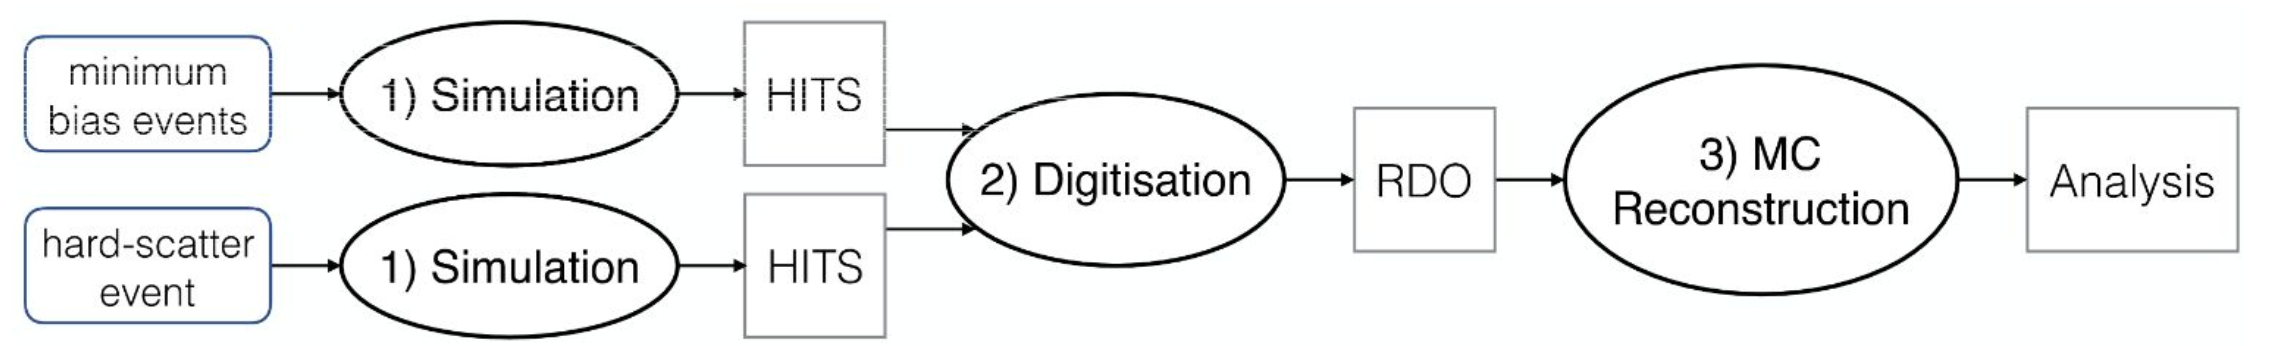
\includegraphics[width=0.9\textwidth]{Chapter2/simulation.png}
	\centering
	\begin{center}
		\caption{The full procedure of the ATLAS simulation}
		\label{Fig:simulation}            
	\end{center}
\end{figure}.


	\let\cleardoublepage\clearpage
 	\chapter{Resonance Searching Strategy}
The resonance search is applying a general strategy with three benchmarks for the exotic particles of different spins: the narrow width approximated scalar boson (NWA, spin=0), the heavy vector triplet (HVT W', Z' bosons, spin=1), and the Randall-Sundrum graviton (RSG, spin=2).
In the study in this thesis, $WW$ and $WZ$ are the two medium states of interest through the production of gluon-gluon fusion, Drell-Yan process, or vector boson fusion. The vector boson fusion is the fusion process of two vector bosons ($W$ or $Z$) emitted from two incoming quarks, and the two quarks are then scattered into two energetic jets with wide $\eta$ separation and high invariant mass. The production processes could be seen in Fig. \ref{Fig:Xprod} as Feynman diagrams. The strategy herein considers only final states in which one $W$ boson decays leptonically ($W\rightarrow l\nu$) into an electron or muon accompanied by a neutrino of the corresponding flavour, while the other $W$ or $Z$ boson is chosen to decay hadronically into two quarks reconstructed into two $R=0.4$ jets or one $R=1.0$ jet ($W/Z\rightarrow jj$ or $W/Z\rightarrow J$). The tau decay channel is not considered in thsi analysis. The benefit of choosing this final state is to have the high branch ratio from the hadronic decay and suppress the QCD contamination by the leptonic side. This study is conducted in a wide range of candidate particle mass ranging from $300GeV$ to $5TeV$. If the mass of a resonance particle is high enough ($m>\tilde1~TeV$), the outcoming two quarks in the final state would be highly boosted, so they cannot not be resolved as two jets with $R=0.4$, and a larger cone of $R=1.0$ is applied to collect their signatures into a single fat jet. 
\\
\\This search was performed with the $36.1fb^{-1}$ data collected by the ATLAS detector in 2015 and 2016 with pp collisions at $\sqrt{s}=13~TeV$. 

\begin{figure}[htp]
	\centering
	\subfloat[Drell-Yan Process]{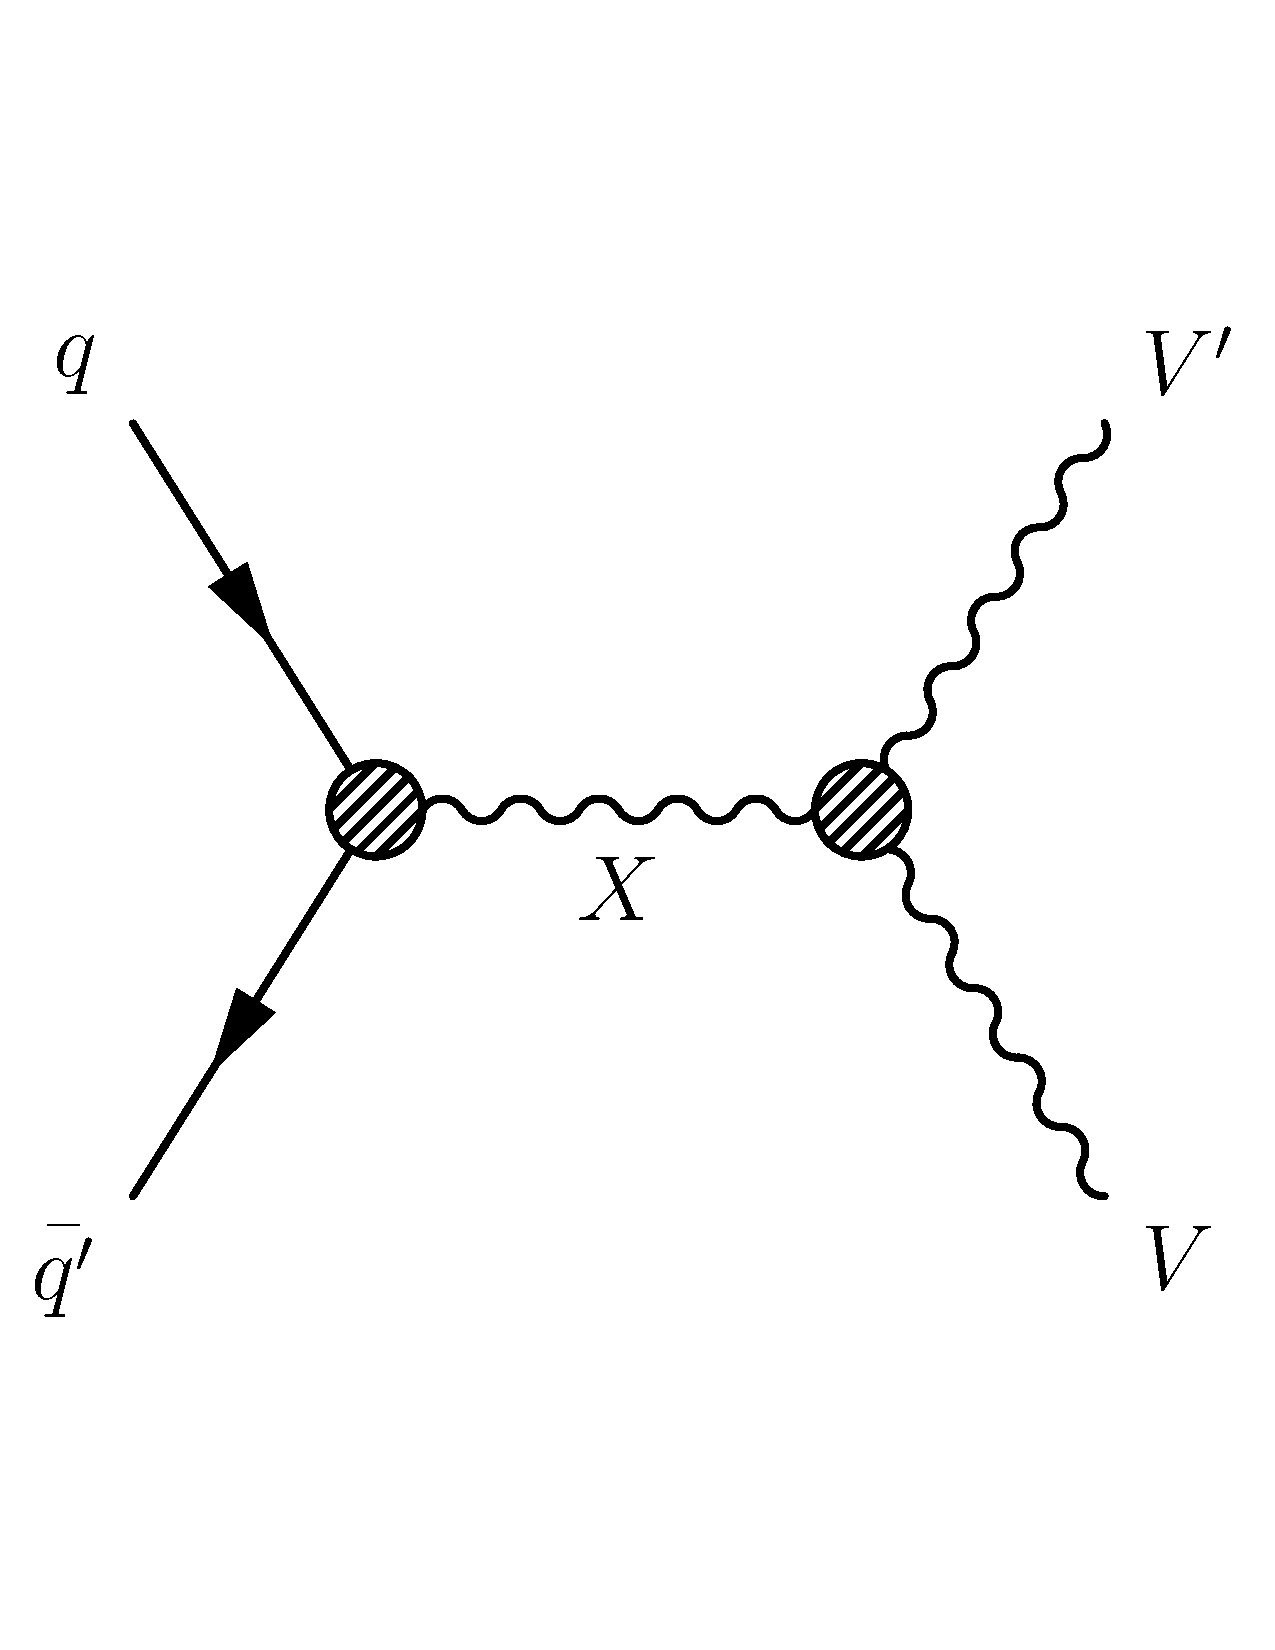
\includegraphics[width=.3\textwidth]{Chapter3/DY_X.pdf}}\hfill
	\subfloat[gluon-gluon Fusion]{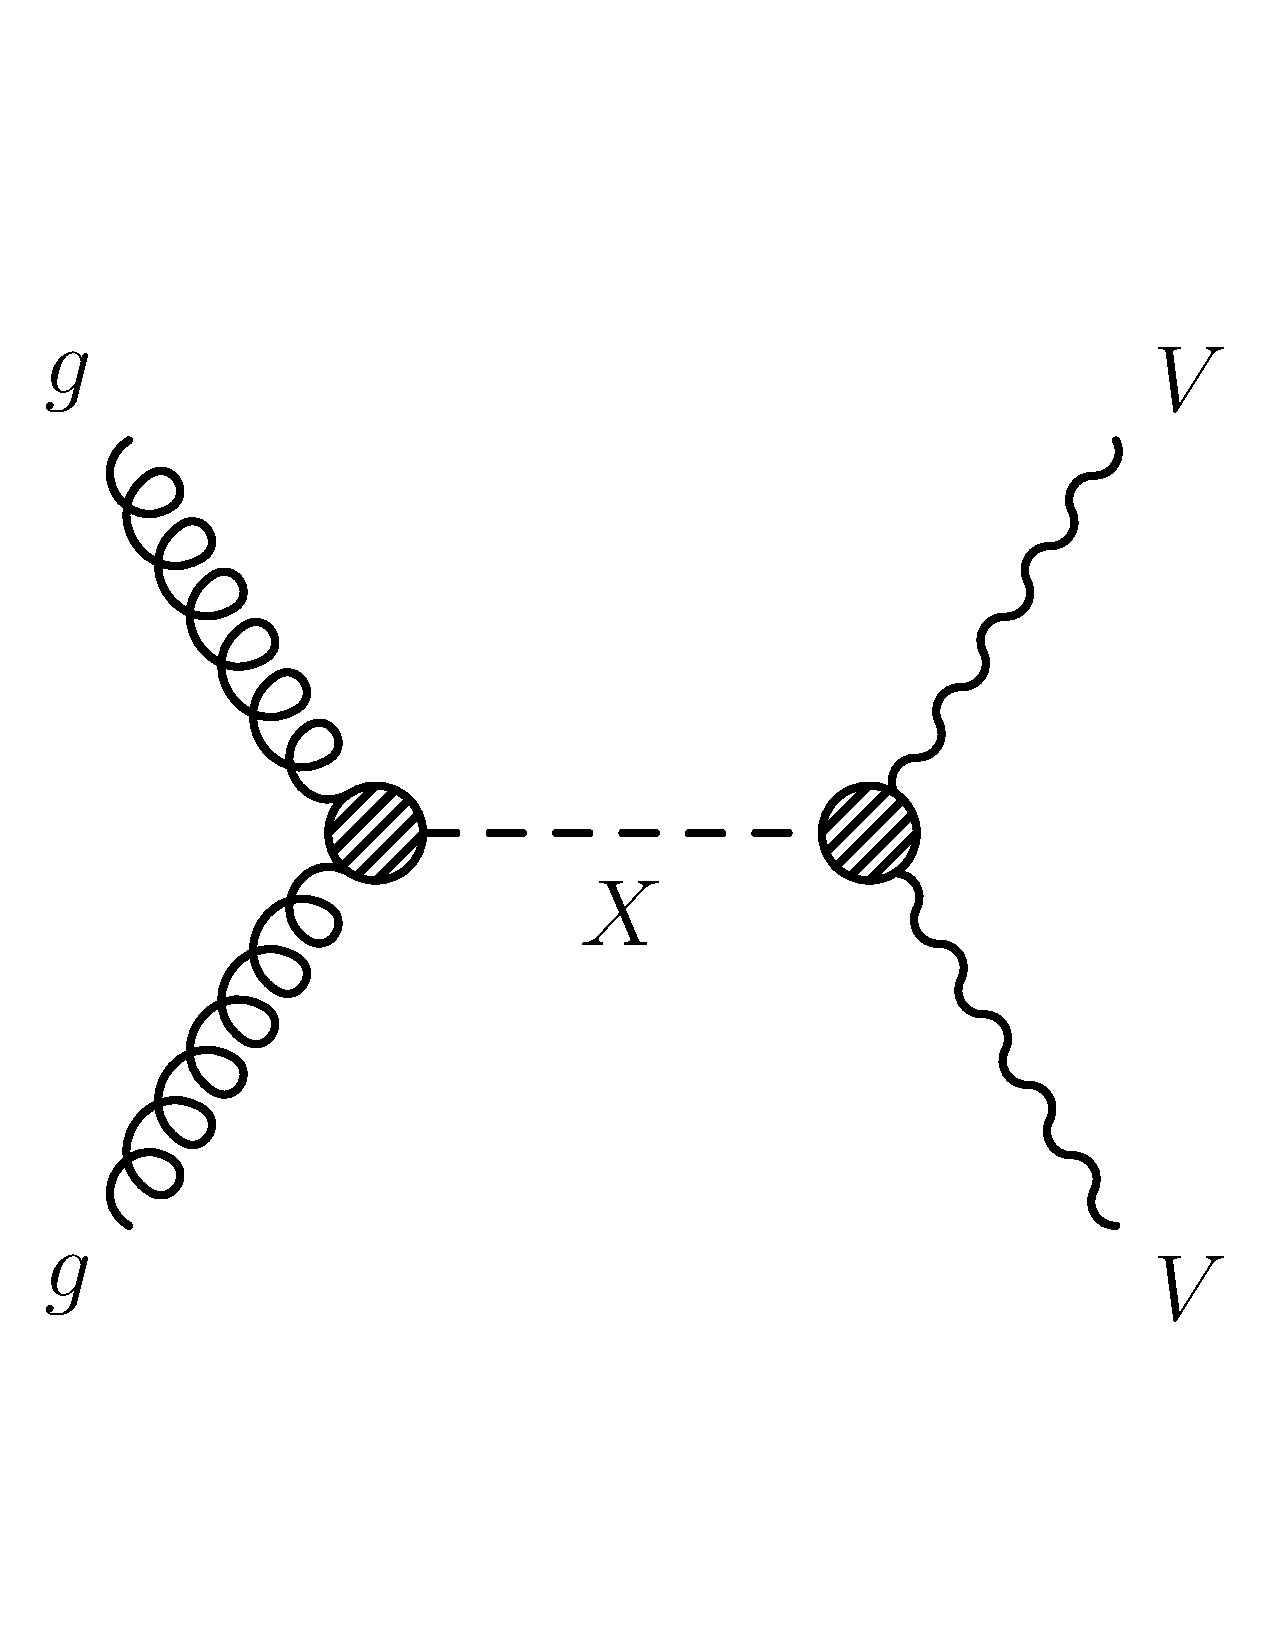
\includegraphics[width=.3\textwidth]{Chapter3/ggF_X.pdf}}\hfill
	\subfloat[Vector Boson Fusion]{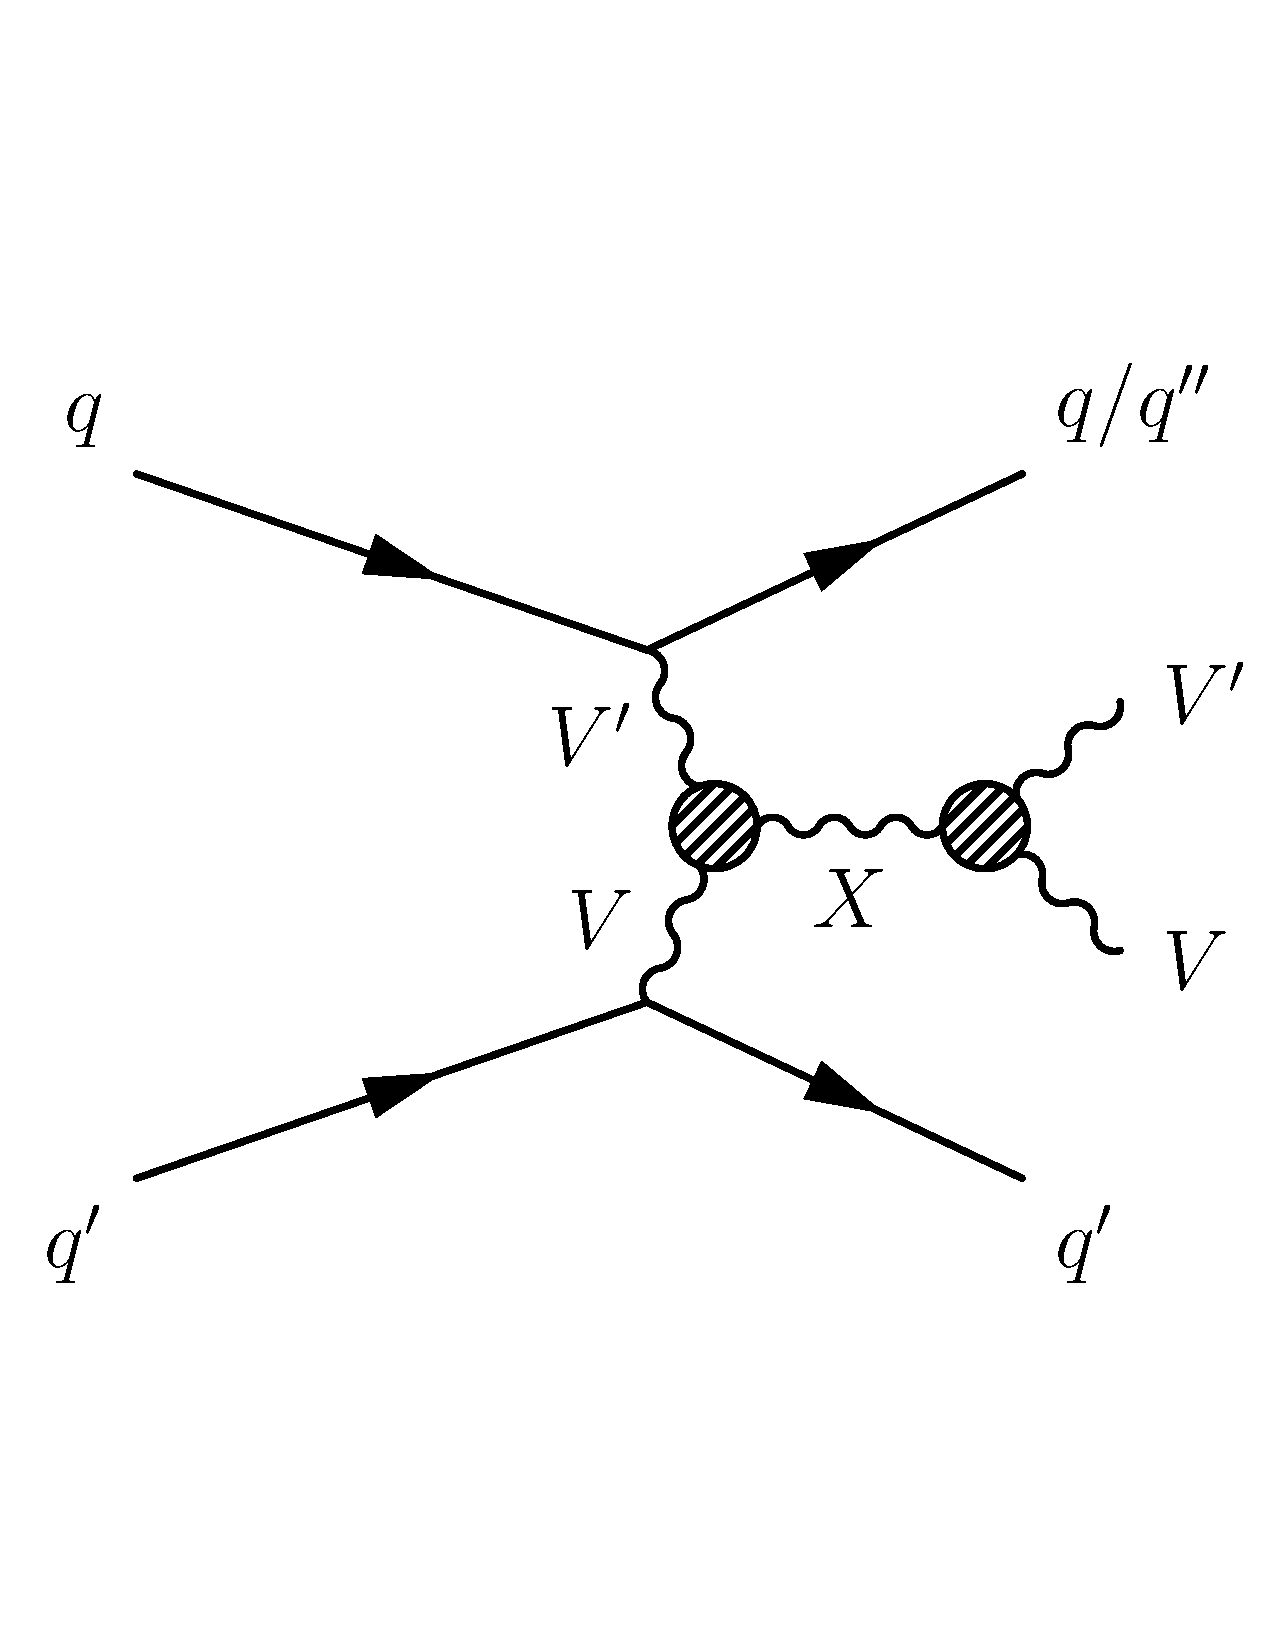
\includegraphics[width=.3\textwidth]{Chapter3/VBF_X.pdf}}
	\caption{The Feynman diagrams of different production mechanisms for particle X which decays into two SM bosons.}
	\label{Fig:Xprod}
\end{figure}
\section{Signal Models}
\label{sec:signal_intro}
In the SM, bosons are the force carriers and also maintain the conservation of certain physical quantities associated with underlying symmetries. To seek for the solution of unsolved problems of the SM, many new models predict the existence of new bosons corresponding to unknown interactions or symmetries, and they also have the strong coupling to the SM bosons which provide the access to verify those theories. However, the existing new models are constructed with many free parameters, and each set of them needs a dedicated analysis from the experimental side, which is impossible in reality. Therefore, a simplified model with only the kinematic parameters related to resonance mass is introduced for which experiments provide precise measurements for on-shell bosons.  
\\
\\This strategy could scan through many models, so it is defined as a general search. However, to give a better separation between signal and background, three benchmarks are applied in this analysis for sensitivity optimization which corresponds to bosons with different spins: $spin=0$, narrow width approximation Higgs bosons (NWA); $spin=1$ heavy vector triplets (HVT); $spin=2$, Randall–Sundrum model gravitons (RSG).
\\
\\{\bf Narrow Width Approximation Higgs Boson}
\\
Some extended models predict the existence of high mass Higgs bosons to solve the problems with the Higgs boson naturalness. However, as only kinematic properties are concerned, the interpretation model chosen in this analysis is the SM Higgs boson but with higher mass. To have further simplification, the decay of the Higgs boson is forced to be always at the mass pole with the narrow width approximation. This means the transferred, $q$, from the proton partons is exactly the mass of the resonant particle under the assumption which gives the narrow resonance width, $\Gamma/m_{H}<<1$, and the interference to the SM Higgs boson is taken negligible. Therefore, the Relativistic Breit–Wigner distribution could be written as:
\begin{equation}
f(q) = \frac{k\pi}{M\Gamma}\delta(q^2-m_{H}^2)
\end{equation}
where $k$ represents:
\begin{equation}
k=\frac{2\sqrt{2}m_{H}\Gamma\gamma}{\pi\sqrt{m_{H}^2+\gamma}}
\end{equation}
and $\gamma=\sqrt{m_{H}^2(m_{H}^2+\Gamma^2)}$. This is then used to evaluate the cross-section of the Higgs boson production.
\\
\\{\bf Heavy Vector Triplet}
\\
\\Heavy vector bosons are predicted by many new BSM theories with the coupling to quarks, leptons, SM vector bosons and Higgs bosons, which constructs a wide phase space to explore. To examine the suitable theories, this study attempts to investigate all the couplings with the set-up of one neutral heavy boson, $Z'$, and two degenerate charged bosons, $W'^{\pm}$, with the given coupling constant, $g_{V}$. For optimization,  two models are taken as the benchmarks. Model A is with an additional symmetry breaking to SM, $SU_{1}(2)\times SU_{2}(2) \times U(1) \rightarrow SU_{L}(2) \times U(1)$ giving a weak coupling: $g_{V} \sim \mathcal{O}(1)$. For the scenario of a strong SM boson coupling, the Minimal Composite Higgs Model is taken as model B with the symmetry breaking, $SO(5) \rightarrow SO(4)$ for $4\pi \geq g_{V} \geq 1$. However, because the decay width is proportional to the coupling constant, and the focus of this search is for the narrow resonance, only $6 \geq g_{V} \geq 1$ is considered with $\Gamma_{V'}/m_{V'}$ below $10\%$.
\\
\\To simplify the models, the coupling strength to all fermions are equal with the scale of $g^2c_{F}/g_{V}$ where $g$ is the $SU_{L}(2)$ gauge coupling, and $c_{F}$ is the dimensionless coefficient between bosons and fermions defined as a free parameters of order one in the phase space of interest. As the fermionic coupling scale is proportional to $1/g_{V}$, model A turns to be more sensitive to the fermionic production with Drell-Yan process, while it is suppressed in model B. In contrast, the coupling to bosons is governed by $c_{H}g_{V}$ with $c_{H}$ as the universal coupling among bosons. Therefore, model B has better sensitivity for higher branch ratio of the decay channel of diboson in this analysis than model A. For the interpretation, the two parameters, $g^2c_{F}/g_{V}$ as well as $c_{H}g_{V}$, construct a two-dimension phase space across which production rates and decay branching ratios vary significantly. 
\\
\\As the coupling to all bosons are the same ($c_{H}g_{V}$), the neutral and charged heavy boson ($Z'$ and $W'^{\pm}$) have the same decay branch ratio to all SM bosons:
\begin{equation}
BR(Z'\rightarrow ZH) = BR(Z'\rightarrow W^\pm W^\pm) = BR(W'^\pm \rightarrow W^\pm Z) = BR(W'^\pm \rightarrow W^\pm H)
\end{equation}
However, with the small mixing angle (between SM and BSM bosons), the coupling in the transverse component is well suppressed, and the dominant contribution is from the longitudinal component. For the same reason, the couplings to neutral dibosons and $W\gamma$ are also so weak that those channels are ignored in this analysis. In the other case, the coupling to $HH$ is forbidden due to the concern of momentum and angular momentum conservation. 
\\
\\{\bf Randall-Sundrum Graviton}
\\
\\To solve the hierarchy problem, extra dimensions were proposed as one of the solutions. It leads to the result that the effective Planck scale, $M_{pl}=2\times10^{18}GeV$, is determined by the existence of extra dimensions from the orginal scale, $M$, and the extra-dimension geometry. The relation between $M_{pl}$ and $M$ is: 
\begin{equation}
\label{Eq:planck_relation}
M_{pl}^{2} = M^{n+2}V_{n}
\end{equation}
where n is the number of dimensions which are not yet observed, and $V$ is the volume constructed from the extra dimensions regardless of the four-dimensional spacetime. Therefore, the visible spacetime is just a manifold under ($4+n$) dimensions.
\\ 
\\Under Randall-Sundrum model, only one more dimension is needed, which hypothesizes that the fifth dimension is constrained with boundary condition of the $\phi$ periodicity ranged between $-\pi$ to $\pi$ called the ``warped bulk'' which bridges two four-dimensional manifolds at $\phi=\pi$  and $\phi=0$ ($\phi$ is taken as the fifth coordinate). The ``Hilbert-Einstein''action under the set-up could be presented as:
\begin{equation}
S = S_{gravity} +S_{obs} + S_{hid}
\end{equation}
\begin{equation}
S_{gravity} = \int d^4x \int^{\pi}_{-\phi}d\phi\sqrt{G}\left[-\Lambda +2M^3R\right]
\end{equation}
\begin{equation}
S_{vis(hid)} = \int d^4x\sqrt{-g_{vis(hid)}}\left[\mathcal{L}_{vis(hid)}-V_{vis(hid)}\right]
\end{equation}
with $\Lambda$ as the cosmological constant, R as the scalar spacetime curvature, and $g$'s are the determinants of metric tensor matrix,  $g_{\mu\nu}$, $V_{vis}$, and $V_{hid}$ are the constant gravitational potentials taken out from the Lagrangian vacuum energy for the visible and hidden spacetimes. After inserting the terms into the Einstein Feild Equation, it leads to the solution for the spacetime description:
\begin{equation}
ds^2=e^{-2\sigma(\phi)}\eta_{\mu\nu}dx^\mu dx^\nu + r_c^2 d\phi^2
\end{equation}
with
\begin{equation}
\sigma(\phi) = kr_c|\phi| \quad k=\sqrt{\frac{-\Lambda}{24M^3}}
\end{equation}
where $\eta$ is the Minkowski metric, and $r_{c}$ is the constant independent of $\phi$ taken as the ``compactification radius'' of the extra dimension on the orbifolding. As a result, the extra dimension only has the dimensional interval, $\pi r_{c}$, at $\phi=\pi$ in the visible spacetime. Taking the space description into Eq. \ref{Eq:planck_relation}, the relation between $r_c$ and $M_{pl}$ could be derived as:
\begin{equation}
M_{pl}^2=\frac{M^3}{k}\left[1-e^{-2kr_{c}\pi}\right]
\end{equation}
This expression indicates that $M_{pl}$ depends on $kr_{c}$, and the weak gravity could be explained with a proper choice of $r_c$. Under the solution, the existence of graviton (the gravitational field) is then taken as the tensor fluctuation on Minkoski metric: $\eta_{\mu\nu} \rightarrow \eta_{\mu\nu}+\bar{h}_{\mu\nu}(x)$. To estimate its mass, the new spacetime geometry is inserted into the Higgs sector in the SM Lagrangian, and it gives the result: $m=e^{-kr_{c}\pi}m_{0}$ with $m_{0}$ as the original mass scale in the visible manifold (IR brane), and m as the one in the five-dimensional spacetime. (This relation could also be applied to SM particles.) If $e^{kr_{c}\pi}$ is of the order $10^{15}$, the mass scale would be in the scale of $TeV$ under the mechanism which offers the signature verifiable to the LHC energy scale with the couplings to SM particles derived from the same way.
\section{Simulation Samples and Derivation}
Each SM background process and each signal sample are simulated by the procedure mentioned in \ref{sec:simulation}.  To make a proper comparison between the simulation and data, the event numbers are normalised to the theoretical cross section and total data luminosity. However, the modelling of interactions between the ATLAS detector and particles is not perfect, and it leads to the discrepancy in efficiency measurements including the particle reconstruction, lepton isolation, trigger, and jet b-tagging efficiency. To recover this disagreement, scaling factors are estimated from the comparison between data and MC and applied on the event weight in the MC samples. 
\\
\\Another disagreement comes from the inconsistency in distribution of interaction number per bunching crossing , $\mu$. To eliminate the effect, one more scale factor is applied through the process called ``pile-up reweighting'' (PRW) to make the simulated $\mu$ distribution agree with data. 
\\
\\After considering all the factors for the data-MC comparison, the final simulation event yield could be reweighted to data by:
\begin{equation}
N_{yield} = \mathcal{L}\times XS \times \epsilon_{rec} \times \epsilon_{iso} \times \epsilon_{trigger} \times \epsilon_{b-tagging} \times \epsilon_{prw} / N_{mc}
\end{equation}
where $N_{mc}$ is the total event weight from simulation, and $\epsilon$'s stand for the scaling factors of different contributions. 
\\
\\{\bf Background Simulation}
\\
\\Some of the SM processes have the same final state to the new physics of our interest: one lepton, one neutrino and multiple jets, and they are called ``irreducible'' background which could not be well-suppressed by selection cuts. This type of backgrounds are estimated from the Monte Carlo simulation contributed from W+jets ($W\rightarrow l\nu$), $t\bar{t}$ ($t\rightarrow bW \rightarrow bjj$ and $t\rightarrow bW \rightarrow bl\nu$), diboson ($WW/WZ\rightarrow l\nu jj$), Z+jets ($Z\rightarrow ll$), and single top interactions.  
\\
\\The events of W/Z+jets are simulated by \textsc{SHERPA} v2.2.1, with the PDF configuration of \textsc{NNPDF30NNLO} as the baseline generator, and the simulation uncertainty is taken by the comparison to other generators detailed in next chapter. With the complicated process of hadronisation including the broad range of jet $p_{T}$ and involved quark flavours, the simulation is done respectively with multiple slices of $max(h_{T}, p_{T}(W/Z))$ ($h_{T}$ is the scalar sum of $p_{T}$ from all jets) and different number of bottom and charm quarks. The involved matrix element for the simulation are up to 2 partons at NLO and 4 partons at LO which is followed by merging into the Sherpa parton shower. The resulting cross section for normalisation is estimated to NNLO of QCD.
\\
\\$t\bar{t}$ events are generated through \textsc{Powheg-Box} v2 with the matrix element calculation provided by \textsc{CT10 PDF} with top quark mass set at $172.5GeV$, and the \textsc{HDAMP} parameters for high $p_{T}$ radiation is set at $1.5m_{t}$. Different from \textsc{SHERPA} as a self-contained generator to do parton shower itself, the simulation from \textsc{Powheg-Box} is then interfaced through \textsc{MadSpin} and \textsc{PYTHIA}8.186 tuned by Perugia 2012 (P2012) and \textsc{CTEQ6L1 PDF} sets for spin correlation preservation of top quark decays and the following parton shower, fragmentation and underlying events. The renormalisation and factorisation scale of the whole process are determined by $\sqrt{m_{t}^2+p^2_{T}(t)}$. The $t\bar{t}$ cross section used for normalisation is calculated using \textsc{TOP++} 2.0 with the precision up to NNLO in QCD. To take in the contribution from soft gluon terms, a re-summation with next-to-next-to-leading logarithmic (NNLL) is applied to make further correction.  
\\
\\Single top events are generated through three processes: s-, t- and Wt-channel productions (Feynman diagrams are presented in Fig. \ref{Fig:singletop}). For the simulation of Wt and s-channels, the same recipe from $t\bar{t}$ generation is adopted, while the t-channel one is through \textsc{Powheg-Box} v1 with fixed four-flavor CT10f4 PDF set but also followed by the same procedure for decay and parton showering from $t\bar{t}$ generation. The renormalisation and factorisation scales are set respectively for the three channels with:
\begin{itemize}
	\item s-channel $\&$ Wt-channel: $m_{t}$
	\item t-channel 4\times$\sqrt{m_{q}^2+p^2_{T}(q)}$ (q is the quark  associated with the single top quark production)
\end{itemize}
, and the cross section for each production is calculated separately with the description in 
\begin{figure}[htp]
	\centering
	\subfloat[t-channel]{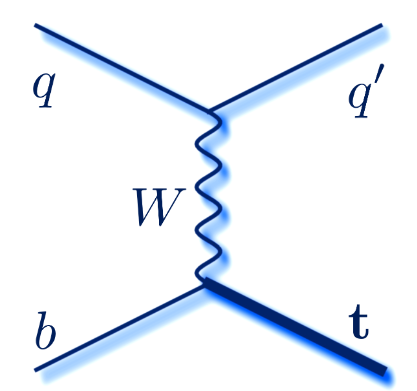
\includegraphics[width=.25\textwidth]{Chapter3/t-channel.png}}\hfill
	\subfloat[Wt-channel]{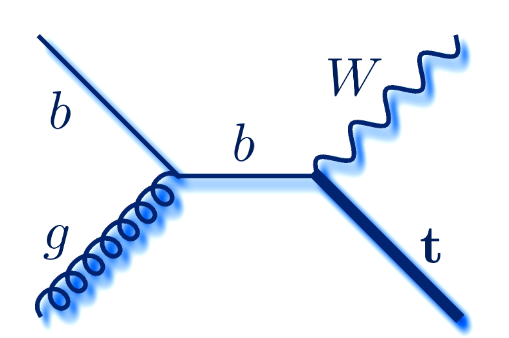
\includegraphics[width=.3\textwidth]{Chapter3/Wt-channel.png}}\hfill
	\subfloat[s-channel]{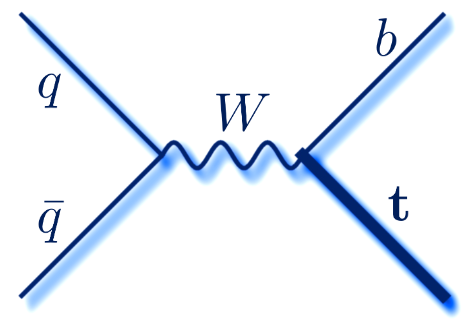
\includegraphics[width=.3\textwidth]{Chapter3/s-channel.png}}
	\caption{The Feynman diagrams of three channels for single top production.}
	\label{Fig:singletop}
\end{figure}

The generation of $WW/WZ$ events are also through \textsc{SHERPA} v2.2.1 for the event production and the hadronisation. 
\\
\\{\bf Signal Simulation}
\\
\\HVT samples are generated via \textsc{MADGRAPH5} interfaced to \textsc{PYTHIA8} with the the resonance mass points ranged from $300~GeV$ to $5~TeV$ of $100~GeV$ spacing. For simplicity, $g_V=1$ and $g_V=3$ are set for model A and model B respectively.
\\
\\RS graviton events are also simulated through \textsc{MADGRAPH5} and \textsc{PYTHIA8}, and only the ggF production is considered for this signal. Within the simulation, $r_{c}=1$ is set as the default for the simulation, but it is also reweighted in the resonance mass distribution at parton level for $r_{c}=0.5$. This is for the comparison with the result from the CMS collaboration. The decay width of this configuration is expected to be $\approx6\%$. 
\\
\\The decay width and cross section of HVT and RS graviton are summarised in tab.~\ref{Tab:xs_decaywidth}. For the NWA Higgs boson, its interference to the SM Higgs boson ($125~GeV$) is assumed to be negligible as discussed in \ref{sec:signal_intro}. Its narrow decay width is set as a constant at $4.07~MeV$ for all mass points which is beyond the experimental resolution with the production of ggF and VBF, which are simulated separately. The simulation is done by \textsc{Powheg-Box} v2 showered with \textsc{PYTHIA8} under \textsc{CTEQ6L1} PDF set. 
\begin{table}[htb]
	\caption{The decay width and cross section of HVT and RSG at $800GeV$, $1.6TeV$, and $2.4TeV$ mass points}
	\centering
		\begin{tabular}{|c|ccc|cc|}
          \hline
          \hline
                   & \multicolumn{3}{c|}{ HVT W' and Z' }                                     & \multicolumn{2}{c|}{ RS $G*$}  \\
              $m$  & $\Gamma$ & $\sigma \times BR(Z' \to WW)$ & $\sigma \times BR(W' \to WZ)$ & $\Gamma$ & $\sigma \times BR(G* \to WW)$ \\
            $[TeV]$& $[GeV]$  & $[fb]$                        & $[fb]$                        & $[GeV]$  & $[fb]$      \\
          \hline
               0.8 & 32       & 354                           & 682                           & 46       & 301   \\
               1.6 & 51       & 38.5                          & 79.3                          & 96       & 4.4 \\
               2.4 & 74       & 4.87                          & 10.6                          & 148      & 0.28 \\
          \hline
         \end{tabular}
	\label{Tab:xs_decaywidth}
\end{table}
\noindent
{\bf Derivation}
\\
\\To boost the computing power, the analyses are not operated on AODs directly, and, instead, they will be going through the ``derivation'' procedure composed of ``trimming'' and ``slimming'' to drop down variables and events of no interest first, which outputs the data format called derived AOD (DAOD). For the broad variety of analysis types, a couple of derivation schemes are applied, and the analyese with similar final states share the same derivation scheme. 
\\
\\With the final state of this analysis, ``HIGG5D2'' is chosen with the derivation scheme as the following:
\begin{itemize}
  \item trigger: passing at least one electron, muon, or $E^{T}_{missing}$ trigger
  \item lepton: one electron or muon with $p_{T}>15~GeV$ 
  \item jet: two small R jets with $p_{T}>20~GeV$, one  small R jet with $p_{T}>100~GeV$, or one large R jet with $p_{T}>150~GeV$
\end{itemize}
\section{Physical Object Definition}
Because the LHC is using protons as the beam source, it leads to the enormous production of hadronic jets. Within the environment, most of other objects suffered great contamination from jet misidentified as other objects. Therefore, the object definitionn for this anlysis is to keep the signal efficiency and significant suppression of misidentification of the intended objects at the same time. 
\\
\\{\bf Electron}
\\
\\The electrons in this analysis are defined as two types, loose and signal, and each event only has exactly one signal lepton without additional loose one. Signal electrons are required to have $p_{T}$ above $27~GeV$ to reach the trigger efficiency turn-on plateau, and $|\eta|<2.47$ is applied on both electron types within the acceptance of inner detector with the crate region vetoed ($1.37<|\eta|<1.52$). The impact parameter requirement is set to only consider the electrons from the primary vertex. The full selection criteria is shown in Tab. \ref{Tab:eledefin}. 
\\
\\In addition to the fundamental quality requirement, the overlap removal is applied afterwards to prevent the objects reconstructed from the same detector signature. When an electron shares inner detector tracks with any muon candidate, the electron is discarded. The existence of a nearby jet defined by $0.2<\Delta R(e,j)<min(0.4,0.04+10/p_{T}(e)[GeV])$ also makes the electron removed. The final requirement on electron is that it shall be consistent with the trigger level electron which fired the required electron trigger to suppress the QCD background. 
\begin{table}[htb]
	\caption{Selection for electron candidates used in the analysis. Veto and signal electrons are defined.}\label{Tab:eledefin}
	\centering
	\begin{tabular}{|c||c|c|}
		\hline
		& \multicolumn{2}{c|}{ Electrons}\\
		&   Loose & Signal \\
		\hline
		$p_T$ & $>7~GeV$ & $>27~GeV$  \\
		\hline
		$| \eta |$ &  \multicolumn{2}{c|}{ $< 2.47 ~ \notin [1.37,1.52]$ } \\
		\hline
		Identification & LooseLH & TightLH   \\
		\hline
		Isolation       &   LooseTrackOnly & FixedCutTight  \\
		\hline
		$|d_0/\sigma(d_0)^{BL}|$ &   \multicolumn{2}{|c|}{  < 5}  \\
		\hline
		$|z_0\sin\theta| $  & \multicolumn{2}{|c|}{< 0.5~mm}  \\
		\hline
	\end{tabular}
\end{table}
\noindent
\\{\bf Muon}
\\
\\Similar to electrons, loose and signal muons are defined with $p_{T}$ and $|\eta|$ cuts in the consideration of trigger turn-on curve plateau and inner detector coverage. The requirement on muon impact parameters is tightened for better rejection to the cosmic muons. The selection criteria is shown below in Tab. \ref{Tab:mudefin}
\\
\\As muons have the lowest misidentification rate, they are kept in most cases for overlap removal. The only exception is the muons decayed from heavy flavour quark, which are called non-prompt muons. To remove this type of contamination, the muons are discarded under the scenarios:
\begin{itemize}
	\item $\Delta R(\mu,j)<0.2$
	\item $\Delta R(\mu,j)<min(0.4,0.04+10~GeV/p_{T}(\mu))$ 
\end{itemize}
\noindent
with the jets fulfilling either of the conditions: a) $p_{T}^{\mu}/p_{T}^j<0.5$ and number of jet-associated tracks greater than 2, b) $p_{T}^{\mu}/\sum^{n}_{1} p_{T}^{trk}<0.7$ for all the jet-associated tracks and $n>2$.
\\
\\The last selection in muon is that it shall be spatially consistent to the trigger muon if muon trigger is fired in the event. 
\begin{table}[htb]
	\caption{Selection for muon candidates used in the analysis. Veto and signal electrons are defined.}\label{Tab:mudefin}
	\centering
	\begin{tabular}{|c||c|c|}
   \hline
& \multicolumn{2}{c|}{Muons}\\
\cline{2-3}
&  Loose & Signal  \\
\hline
$p_T$ threshold &  7~GeV & 27~GeV  \\
\hline
$| \eta |$      &  $< 2.7$ & $< 2.5$   \\
\hline
Identification  &  Loose & Medium  \\
\hline
%Track Quality   &  - & - & ''Loose Muon'' & ''Loose Muon'' \\
Isolation       &   LooseTrackOnly & FixedCutTightTrackOnly  \\
\hline
$|d_0/\sigma(d_0)| w.r.t. BL$ &   \multicolumn{2}{|c|}{< 3} \\
\hline
$|z_0\sin\theta| $ &   \multicolumn{2}{|c|}{< 0.5~mm} \\
\hline
	\end{tabular}
\end{table}
\noindent
\\{\bf Small R Jets [R=0.4]}
\\
\\In the intended final states, the jets (denoted as $j$) come from the decay of W bosons ($W\to jj$) or the remnant quarks from the vector boson fusion ($jj\to WWjj$ or $jj \to WZjj$). Because of the kinematic properties, the two types of jets are selected respectively. The full selection criteria are in Tab. \ref{tab:sjdefinit}.
\\
\\The pair of VBF jets are supposed to be a high mass dijet system with wide separation, so they have tighter $p_{T}$ selection of $p_{T}>30~GeV$ but looser $|\eta|$ cut, $|\eta|<4.5$. For signal jets, they are only required to have $p_{T}>20~GeV$, and only the ones within the acceptance of inner detector ($|\eta|<2.5$) are taken as jet candidates for event selection. The jet quality requirement is to remove the ``fake jets'' from calorimeter noise pulse, cosmic ray, or non-collision background (like beam-halo), which is called ``jet cleaning''.

\begin{table}[tbh]
	\caption{Selection for small-R jets}\label{tab:sjdefinit}
	\vspace{2.0em}
	\centering
	\begin{tabular}{|c||c|c|}
		\hline
		             & \multicolumn{2}{|c|}{ Small-R Jets }\\
		\hline
		             & Signal Jets & VBF Jets \\
		\hline
		Algorithm    & \multicolumn{2}{|c|}{ anti$-k_t$, $R=0.4$}\\
		\hline
		$p_T$        & $>20~GeV$ & $>30~GeV$\\
		\hline
		|$\eta$|     & $< 2.5$ & $<4.5$  \\
		\hline
		Quality      & \multicolumn{2}{|c|}{not ``bad'' jet}\\
		\hline
		JVT          & \multicolumn{2}{|c|}{$< 0.59$ ( $| \eta | < 2.4 ~ \& \& ~p_T < 60 $ GeV)} \\
		\hline
		b-Tagging    & \multicolumn{2}{|c|}{\texttt{MV2c10}, 85\% efficiency} \\
		\hline
	\end{tabular}
\end{table}
\noindent
{\bf Large R Jets [R=1.0]}
\\
\\When the W or Z boson is highly boosted decayed from a heavy particle, the outcoming quarks would be close to each other. In this case the small R jets would not have enough resolution power to reconstruct them individually, so the large R jets (or called ``fat jets'' and denoted as $J$) are reconstructed to collect the energy deposits from the close-by quarks. The full selection on the fat jets could be seen in Tab. \ref{Tab:Jdefinit}. With this topology, the jet mass and $p_{T}$ would need the further correction. This is performed with the track-assisted mass, $m^{TA}$, as the calorimeter cannot provide enough spatial resolution. $m^{TA}$ is estimated from the tracks left by charged jet partons inside the fat jets defined as:
\begin{equation}
m^{TA} = m^{trk} \times \frac{p_{T}^{J}}{\sum p_{T}^{trk}}
\end{equation}  
Here, $m^{trk}$ is the reconstructed mass of the tracks taken as massless particles, and $p_{T}^{trk}$ is the vector sum from $p_{T}$ of tracks.  The ratio of $p_{T}$ between tracks and the jet is to take in the neutral-to-charge fluctuations. It could then be combined with the calorimeter mass, $m^{calo}$, into the combined mass, $m^{comb}$, by this definition:
\begin{equation}
m^{comb} = \frac{\sigma_{{calo}}^{-2} m^{{calo}} + \sigma_{{TA}}^{-2} m^{{TA}} }{\sigma_{{calo}}^{-2} + \sigma_{{TA}}^{-2}}
\end{equation}
with $\sigma_{{calo}}^{-2}$ and $\sigma_{{TA}}^{-2}$ as pre-estimated mass resolutions for  the calorimeter and track-assisted mass which are assumed to be uncorrelated. From Fig. \ref{Fig:combinedmassperformance}, it could be seen that the calorimeter mass has better performance in the low $p_{T}(W)$ regime benefited from the great energy resolution, but it is degraded as $p_{T}(W)$ increases, while the track-assisted mass performed in an opposite way. The combined mass takes the merits of these two mass definitions and provide the best mass resolution ($\sim10\% (15\%)$ at jet $p_{T}=1TeV(2.5TeV)$). It is taken as the nominal fat jet mass in this analysis with the selection of $m^{comb}>50GeV$. The jet $p_{T}$ is the corrected by $p_{T}^{comb}=p_{T}^{calo}\times m^{comb}/m^{calo}$ 

\begin{table}[h]
	\caption{Selection for large-R jets}\label{Tab:Jdefinit}
	\vspace{2.0em}
	\centering
	\begin{tabular}{|c||c|}
		\hline
		& Signal Large-R Jets\\
		\hline
		Algorithm & anti$-k_t$, $R=1.0$\\
		$p_{T}$   & >200~GeV\\
		$| \eta |$      & $< 2.0 $\\
		Mass threshold  & 50~GeV\\
		W/Z Tagger &  $D^{\beta =1}_2 \& m^{comb}$ \\
		\hline
	\end{tabular}
\end{table}
\begin{figure}[ht]
	\begin{center}
		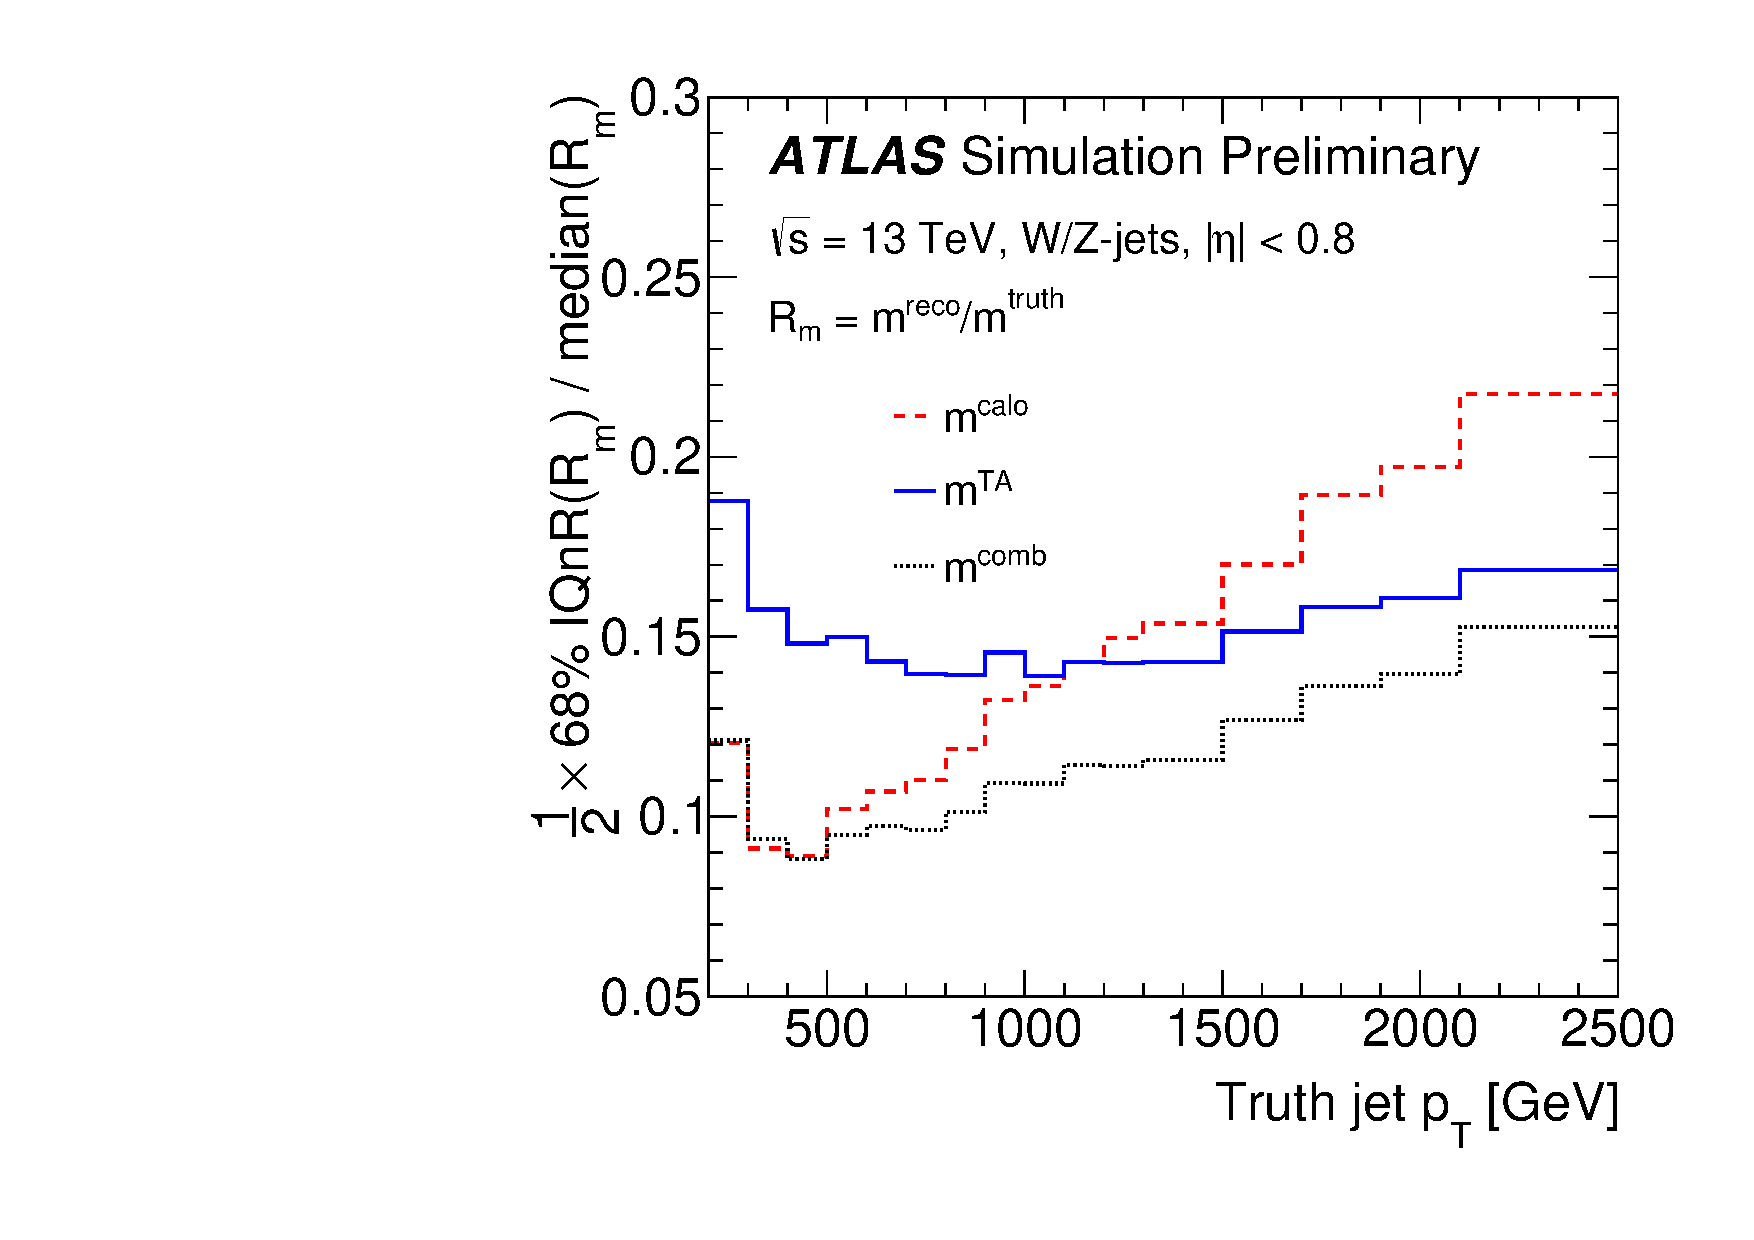
\includegraphics[width=0.6\hsize]{Chapter3/mass_resolution}
		\caption{The jet mass resolution as a function of jet $\p_{T}$ for jets produced from boosted $W$ boson\cite{ATLAS-CONF-2016-035}. Three different jet mass reconstruction algorithms are displayed: the calo-jet mass ($m^{{calo}}$), the track-assisted mass ($m^{{TA}}$), and the combined TA+calo mass ($m^{{comb}}$).}
		\label{Fig:combinedmassperformance}
	\end{center}
\end{figure}
\noindent
However, the combined mass is still not proficient to select the W/Z decayed fat jets precisely, so the substructure of jets is needed to improve the boson tagging. This extra information is extracted with the subjets of $R=0.2$ from a $k_{T}$ algorithm performed on the topoclusters. Those tiny jets are then taken as the new entities to be ``ghost-associated'' with the fat jets through the $anti-k_{T}$ algorithm with the threshold on $p_{T}$, $p_{T}^{R=0.2}/p_{T}^{R=1.0}>0.05$. The jet substructure information could then be give by the discriminant, $D^{\beta =1}_{2}$, for W/Z boson recognition which is defined as:
\begin{equation}
D^{\beta =1}_{2} = \frac{e^{\beta}_{3}}{e^{\beta}_2} 
\end{equation}
with $e^{\beta}_{2}$ and $e^{\beta}_{3}$ as:
\begin{equation}
e^{\beta}_{2} = \frac{1}{(p_{T}^{jet})^2}\displaystyle\sum\limits_{i<j\in J}p_{T}^{i}p_{T}^j(R_{ij})^{\beta}
\end{equation}
\begin{equation}
e^{\beta}_{3} = \frac{1}{(p_{T}^{jet})^3}\displaystyle\sum\limits_{i<j<k\in J}p_{T}^{i}p_{T}^{j}p_{T}^{k}(R_{ij}R_{jk}R_{ik})^{\beta}
\end{equation}
where i, j, and k are the index for the subjets. The boson tagging is then done by a 2D cut on both $D^{\beta =1}_{2}$ and $m^{comb}$ as a function of $p_{T}$ shown in Fig. \ref{Fig:newWZtaggerWP} with two working points, $50\%$ and $80\%$, for the tagging efficiency. 
\begin{figure}[ht]
	\begin{center}
		\subfloat[]{
			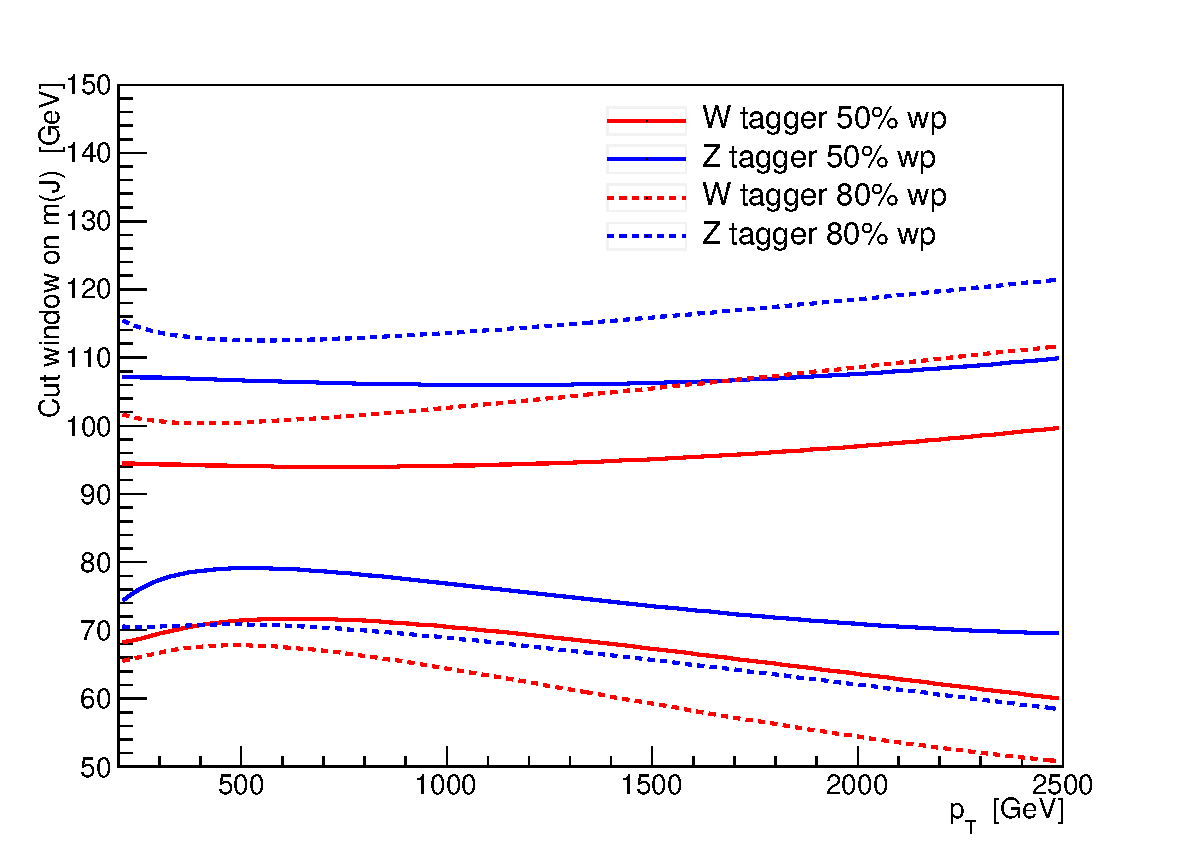
\includegraphics[width=0.48\hsize]{Chapter3/MassWindow_newWZTagger}
		}
		\subfloat[]{
			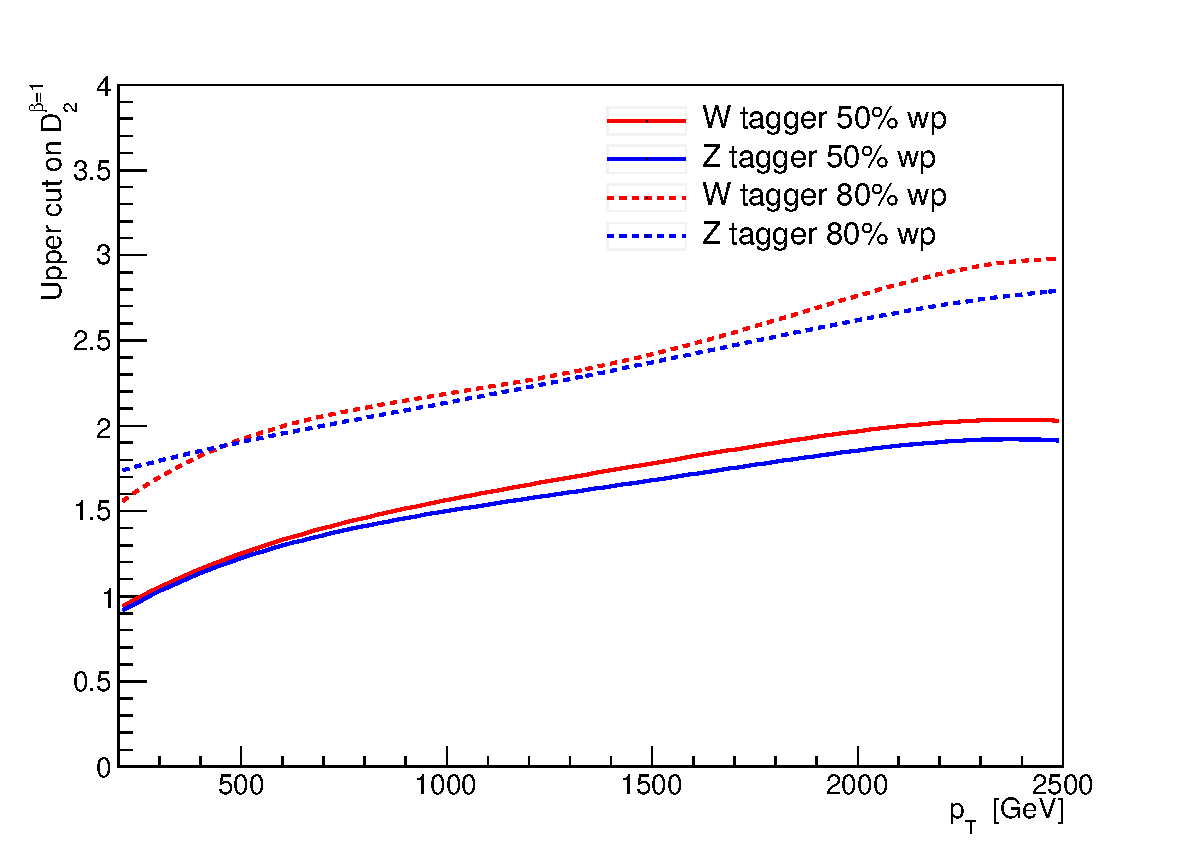
\includegraphics[width=0.48\hsize]{Chapter3/D2UpperCut_newWZTagger}
		}
		\caption{The thresholds of the mass window cut (a) and the upper cut on $D^{\beta =1}_2$ (b) as a function of $p_{T}$ used in this analysis. The cuts  for $W$-($Z$)-boson tagging is shown by red (blue) lines.}
		\label{Fig:newWZtaggerWP}
	\end{center}
\end{figure}
\noindent
\\{\bf Missing Transverse Energy}
\\
\\Although $E^{missing}_{T}$ is supposed to be reconstructed as shown in Sec. \ref{sec:obj rec}, hadronically decayed taus and photons are treated as jets for the intended final state in this analysis. The reason is that they are not considered in the 
\\
\\The cut on $E^{miss}_{T}$ will be discussed in the next section.   
\section{Event Selection}
The event selection is conducted to maximize the sensitivity by removing background events but also keeping the signal at the same time. To achieve this purpose, the significance is defined as:
\begin{equation}
\label{Eq:significance}
\sigma_{sig} = \displaystyle\sum_{i}^{N_{bin}}( \frac{s_i}{s_i+b_i+(\Delta_bi)^2})^2
\end{equation}
where $s_i$ and $b_i$ are the signal and background event numbers. The cuts on variables would be varied on signal and background samples simultaneously, and the final criteria is given by the combination of cuts giving the best significance. The signal sample applied in the optimization could be either via the medium state of WW or WZ, as they have similar kinematic properties. However, they are still divided into two subchannels with the definitions for dedicated mass windows.  
\\
\\Then, the events in this analysis are further categorized by jet topologies and VBF jet selection. In general, the VBF categories could gain better sensitivity than the ggF/DY production ones, and the events with fat jets which are called ``boosted'' events are also more sensitive than the resolved signal regions. Fig. \ref{Fig:order} shows how the events are categorized, and the categories with better sensitivity to the signal are given high priorities (boosted $>$ resolved, VBF $>$ ggF/qqF). For the events which fail part of the jet selection, they would go into the control regions to constrain the background contribution from W+jets and $t\bar{t}$ which are the two dominant backgrounds in this analysis. The two control regions are used in the simultaneous fitting to derive the scale factor of background estimation, and the details will be discussed in the next chapter
\begin{figure}[h]
	\centering
	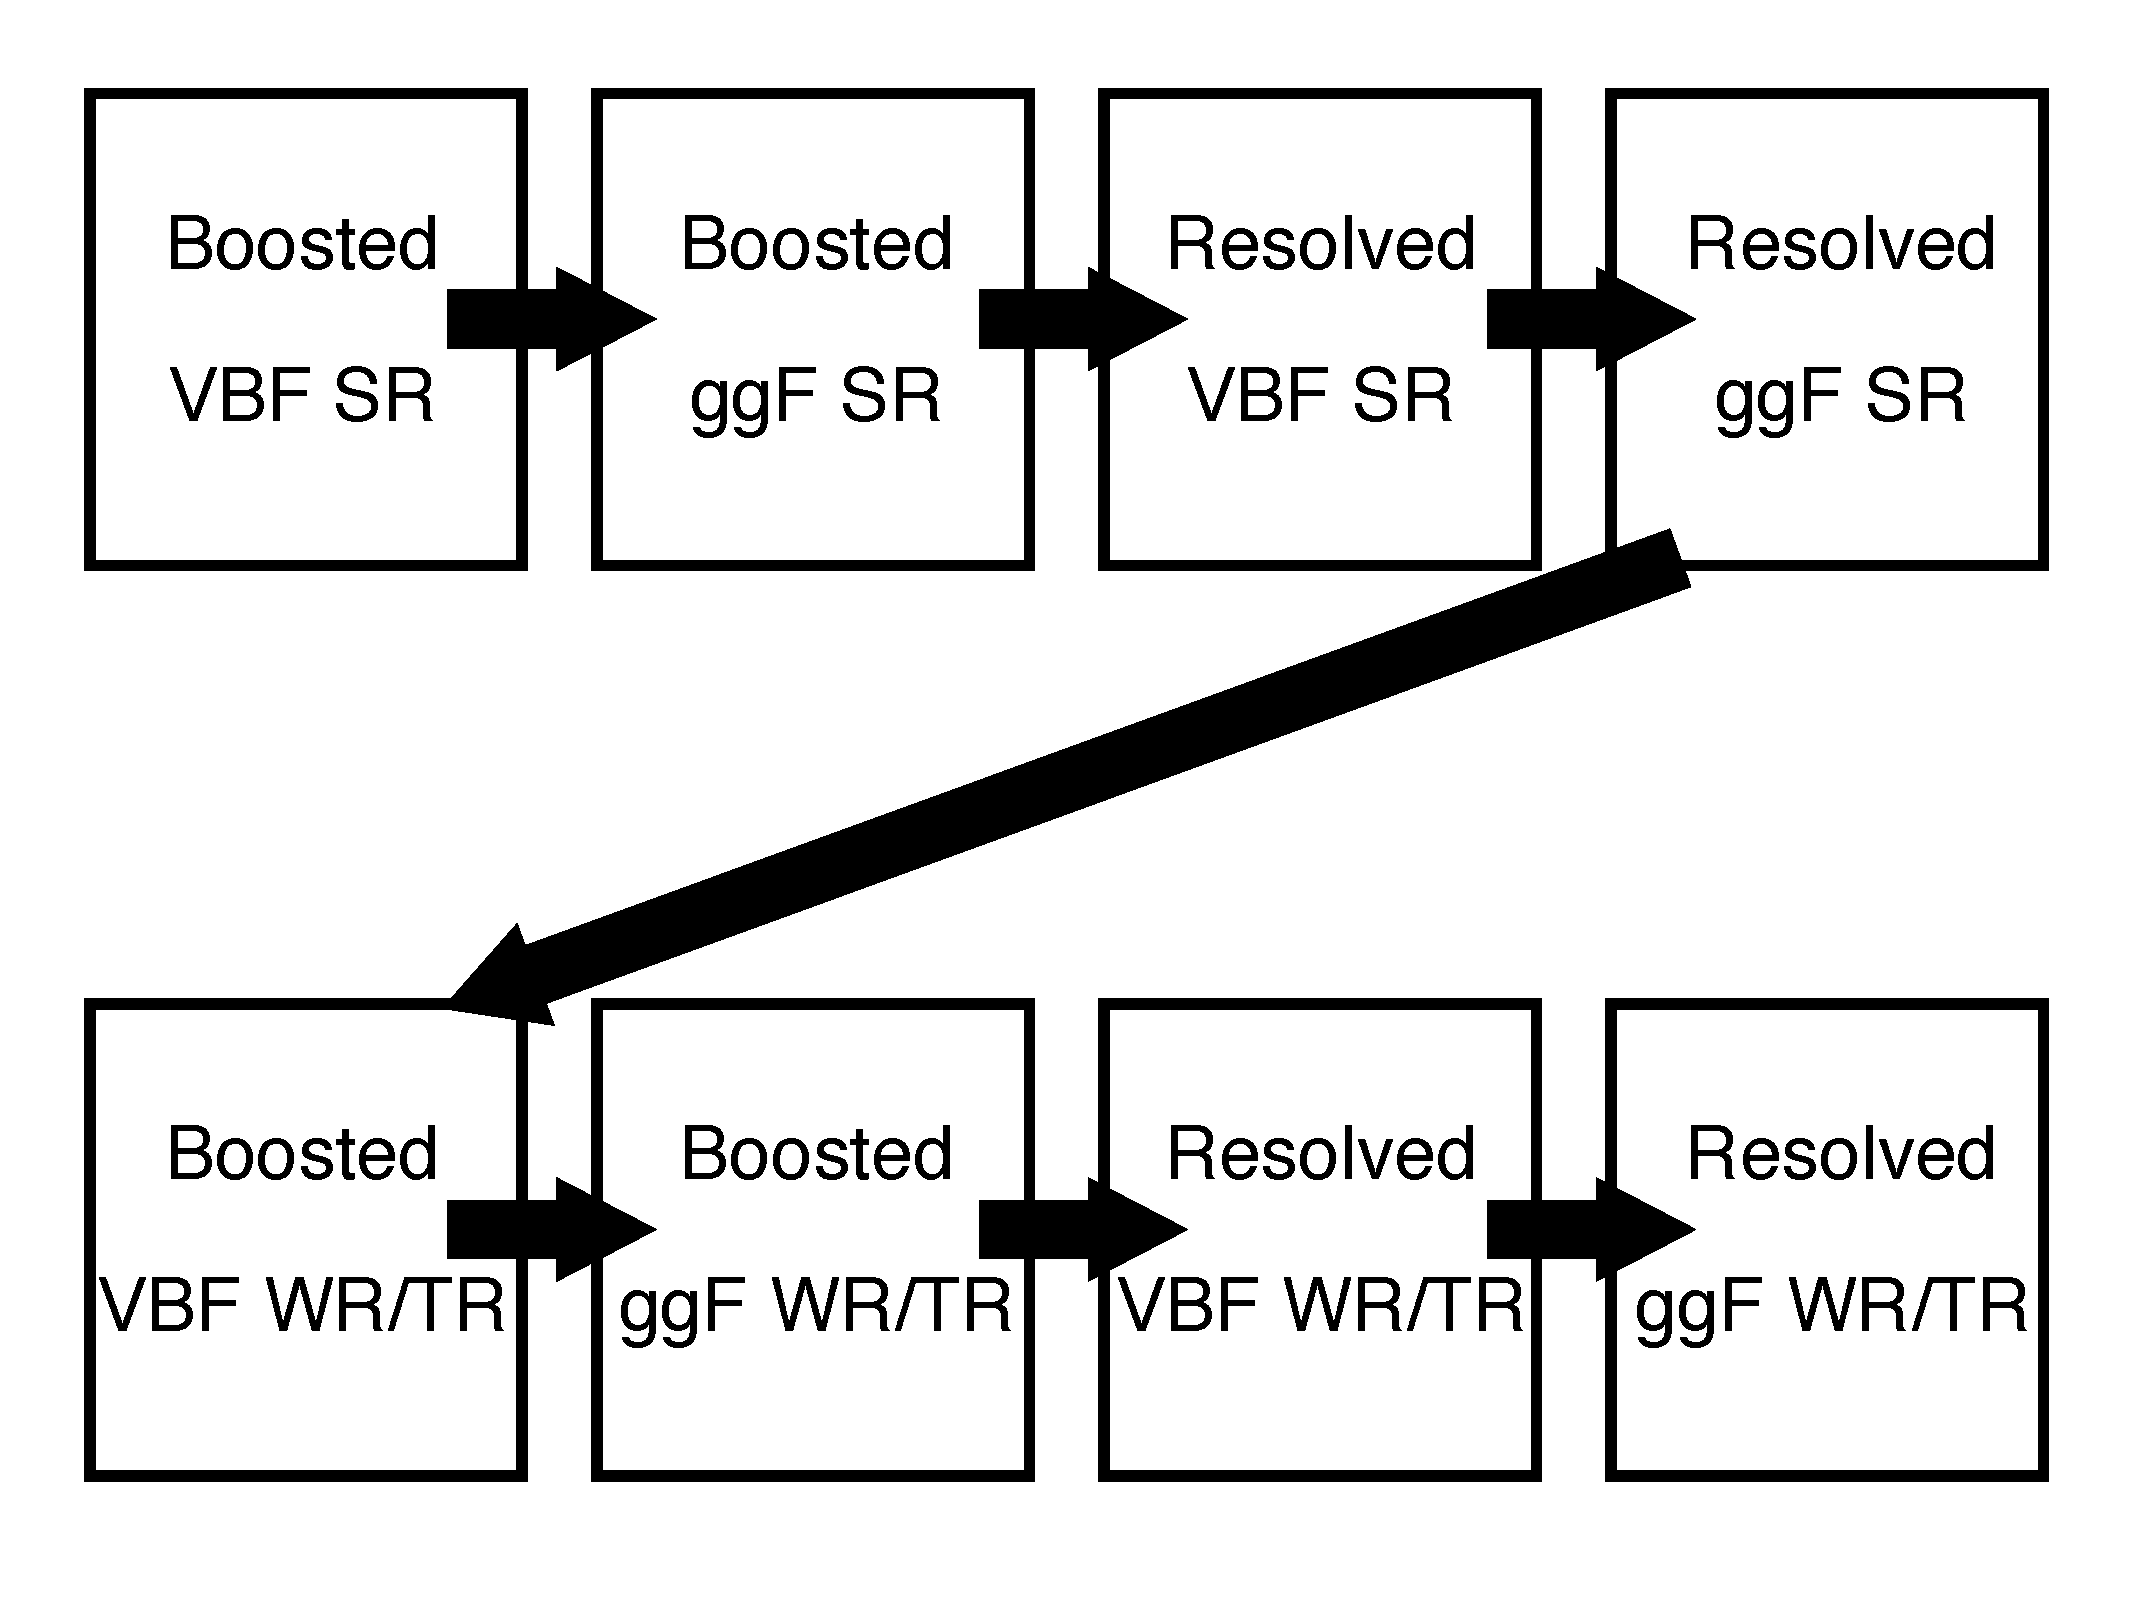
\includegraphics[width=0.7\hsize]{Chapter3/order}
	\caption{Illustration of how to combine the SR/CRs in this analysis.}
	\label{Fig:order}
\end{figure}

\subsection{Trigger}
\label{Subsec:Trigger_resonance}
The first applied criterion on event selection is the trigger. The recorded data is a broad collection of different physical signatures, and our final state only accounts for a small fraction of them. Because of the increasing luminosity provided by LHC, the trigger thresholds were enhanced in 2016 to reduce the trigger rate. For the MC samples, the run number is randomly generated, and the events shall only pass the triggers available in the random run number. The full trigger set used in this analysis is shown in Tab. \ref{tab:triggers}
\begin{table}[h]
	\caption{The list of triggers used in the analysis.} \label{tab:triggers}
	
		\footnotesize
		\begin{center}
		\begin{adjustbox}{center}
			\begin{tabular}{|l|c|c|c|}
				\hline
				\multirow{2}{*}{Data-taking period} & \multirow{2}{*}{Electron channel} & \multicolumn{2}{c|}{ Muon channel }  \\
				\cline{3-4}
				& & $p_{T},\left(\mu\nu\right) < 150\,GeV$ & $P_{T},\left(\mu\nu\right) > 150\,GeV$   \\
				\hline
				\multirow{3}{*}{\centering {2015}} & HLT\_e24\_lhmedium\_L1EM20 & HLT\_mu20\_iloose\_L1MU15 & \multirow{3}{*}{ HLT\_xe70 } \\
				& HLT\_e60\_lhmedium  & HLT\_mu50 & \\
				& HLT\_e120\_lhloose & & \\
				\hline
				\multirow{2}{*}{\centering {2016a (run $< 302919$)}} & HLT\_e26\_lhtight\_nod0\_ivarloose & HLT\_mu26\_ivarmedium  & \multirow{3}{*}{ HLT\_xe90\_mht\_L1XE50 } \\
				& HLT\_e60\_lhmedium\_nod0 & HLT\_mu50 &  \\
				($L<1.0\times10^{34}\,{ cm}^{-2}\,{s}^{-1}$) & HLT\_e140\_lhloose\_nod0 & & \\
				\hline
				{\centering {2016b (run $\geq 302919$)}} & \multirow{2}{*}{same as above} & \multirow{2}{*}{same as above}  &  \multirow{2}{*}{HLT\_xe110\_mht\_L1XE50} \\
				($L<1.7\times10^{34}\,{ cm}^{-2}\,{ s}^{-1}$) & & &\\
				\hline
				\hline
				Total int. lumi. [$fb^{-1}$] &  36.1 & 35.6 & 35.9 \\
				\hline
			\end{tabular}
		\end{adjustbox}
		\end{center}
	
\end{table}
\noindent
\\Three electron triggers are used in electron channel including the unprescaled lowest threshold one to maximize the signal efficiency. The other two triggers are used to select high $\p_{T}$ electrons with looser isolation requirement. The combined performance of the triggers is around $90\%$ efficiency at the turn-on plateau as a function of $p_{T}$.
\\
\\In muon channel, both $E_{T}^{miss}$ and muon triggers are used. For the scenario of $p_{T}(\mu\nu)<150~GeV$, the unprescaled lowest threshold muon trigger is used accompanied by the higher threshold one without any isolation requirement. Otherwise, $E^{T}_{miss}$ trigger is chosen for $p_{T}(\mu\nu)>150~GeV$ events because muon trigger can only reach $70\%$ efficiency on the plateau.
\\
\\However, the $E^{miss}_{T}$ cut in this analysis is below the plateau, so there might be the inconsistency between data and simulation in terms of the efficiency. Therefore, ``tag and probe'' method is applied to study the trigger efficiency as a function of $p_{T}(\mu\nu)$ (because muons are invisible in trigger level, trigger level $E_{T}^{miss}$ is actually $p_{T}(\mu\nu)$). This study is performed on boosted and resolved channels respectively. The tagged events are required to fulfil the following conditions for the resolved (boosted) channel: a) one muon with $p_{T}>27~GeV$ b) $E^{miss}_{T}>60(100)~GeV$ c) at least 2 signal jets (1 fat jet) selected d) the unprescaled lowest threshold muon trigger is fired. The events are then probed by whether $E^{miss}_{T}$ trigger is fired to give the efficiency. The result for data and simulated $t\bar{t}$ events are shown in Fig. \ref{Fig:eff_met_merged} for boosted channel in Fig. \ref{Fig:eff_met_resolved} for the resolved channel. The efficiency reaches the plateau at $200~GeV$, but $E^{miss}_{T}$ trigger is applied for $p_{T}(\mu\nu)>150~GeV$, so the scaling factor is taken into simulation as the extra event weight to make them consistent. 
\begin{figure}[ht]
	\begin{center}
		\subfloat[]{
			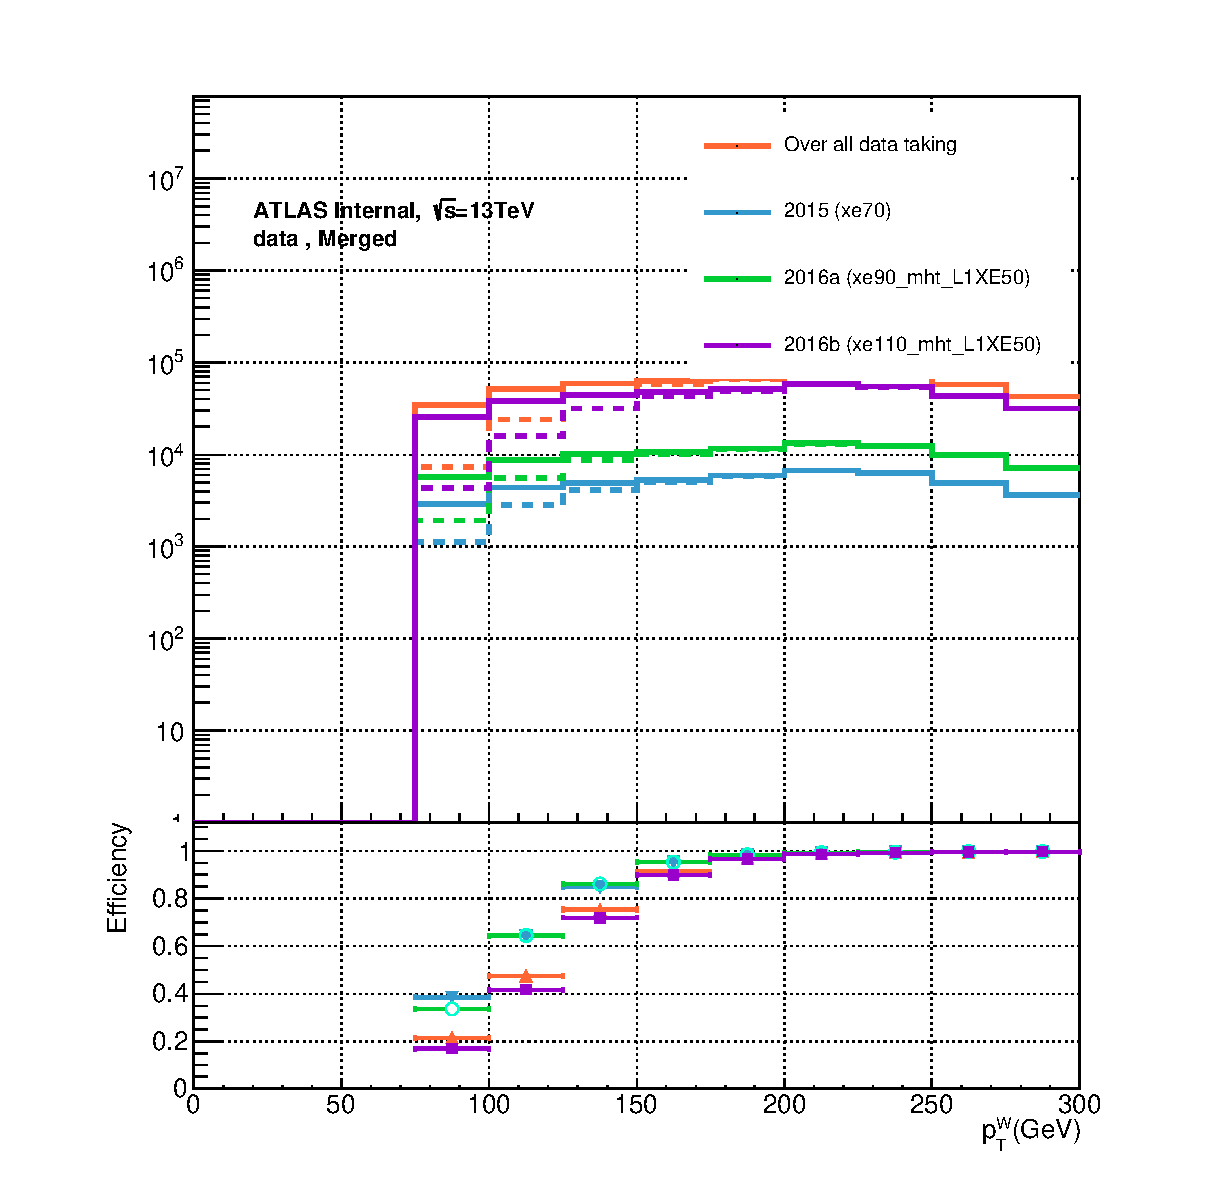
\includegraphics[width=0.48\hsize]{Chapter3/Merged_TrigEff_ptW_METcut_data.eps}
		}
		\subfloat[]{
			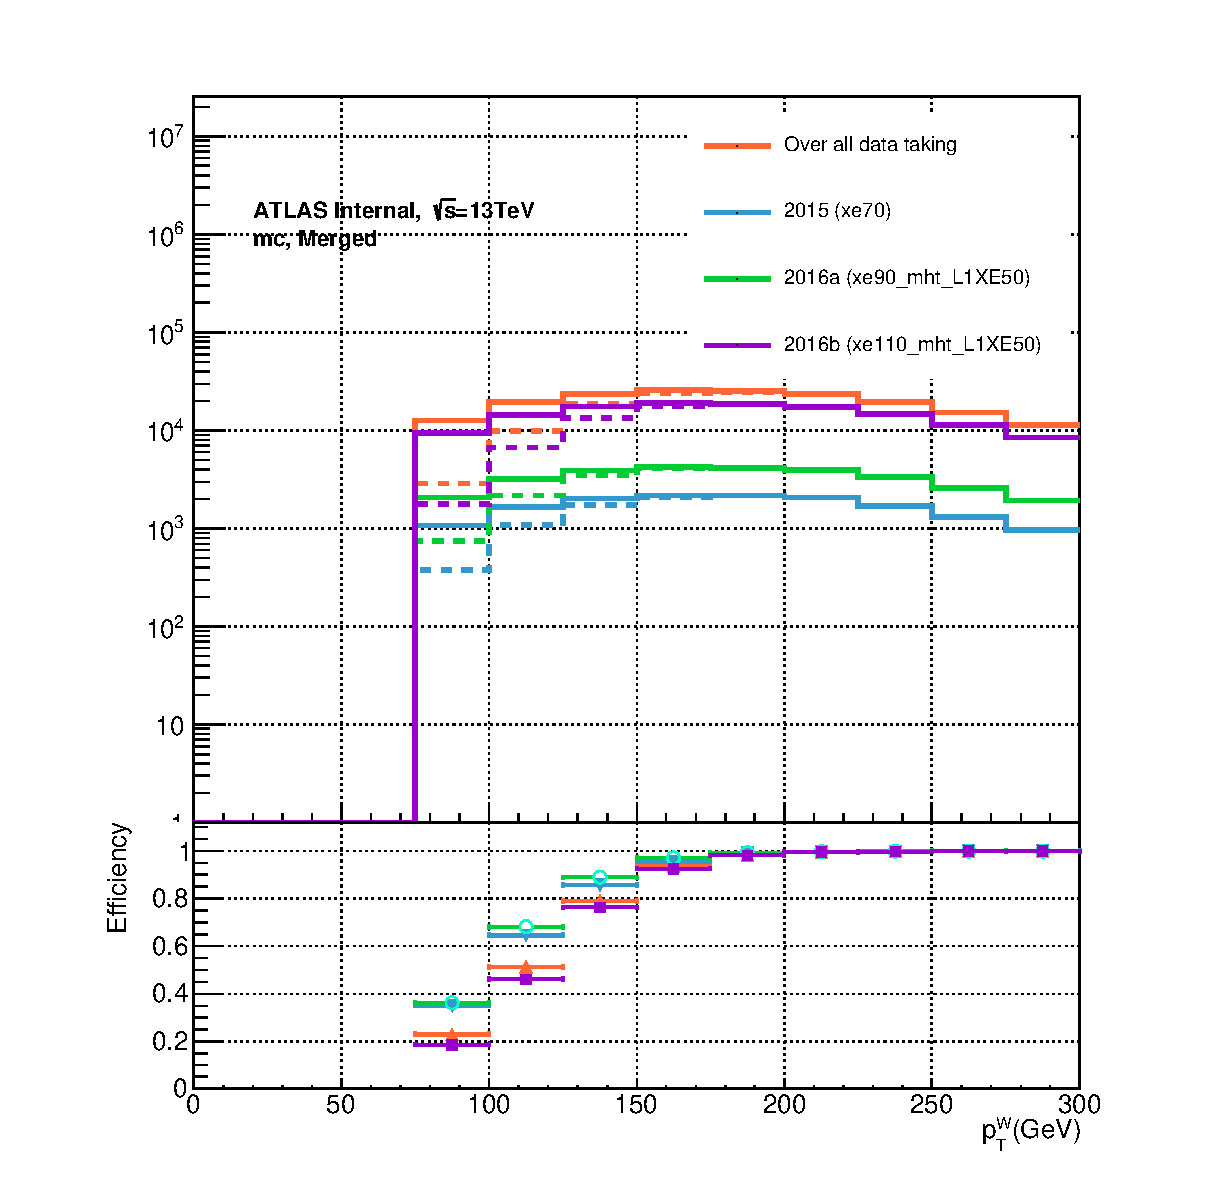
\includegraphics[width=0.48\hsize]{Chapter3/Merged_TrigEff_ptW_METcut_ttbar.eps}
		}
		\caption{The upper plot is $p_{T}(\mu\nu)$ distribution of tagged (real) and probed events in boosted channel for data (a) and $t\bar{t}$ events (b). The lower plots is the efficiency as a function of $p_{T}(\mu\nu)$}
		\label{Fig:eff_met_merged}
	\end{center}
\end{figure}

\begin{figure}[ht]
	\begin{center}
		\subfloat[]{
			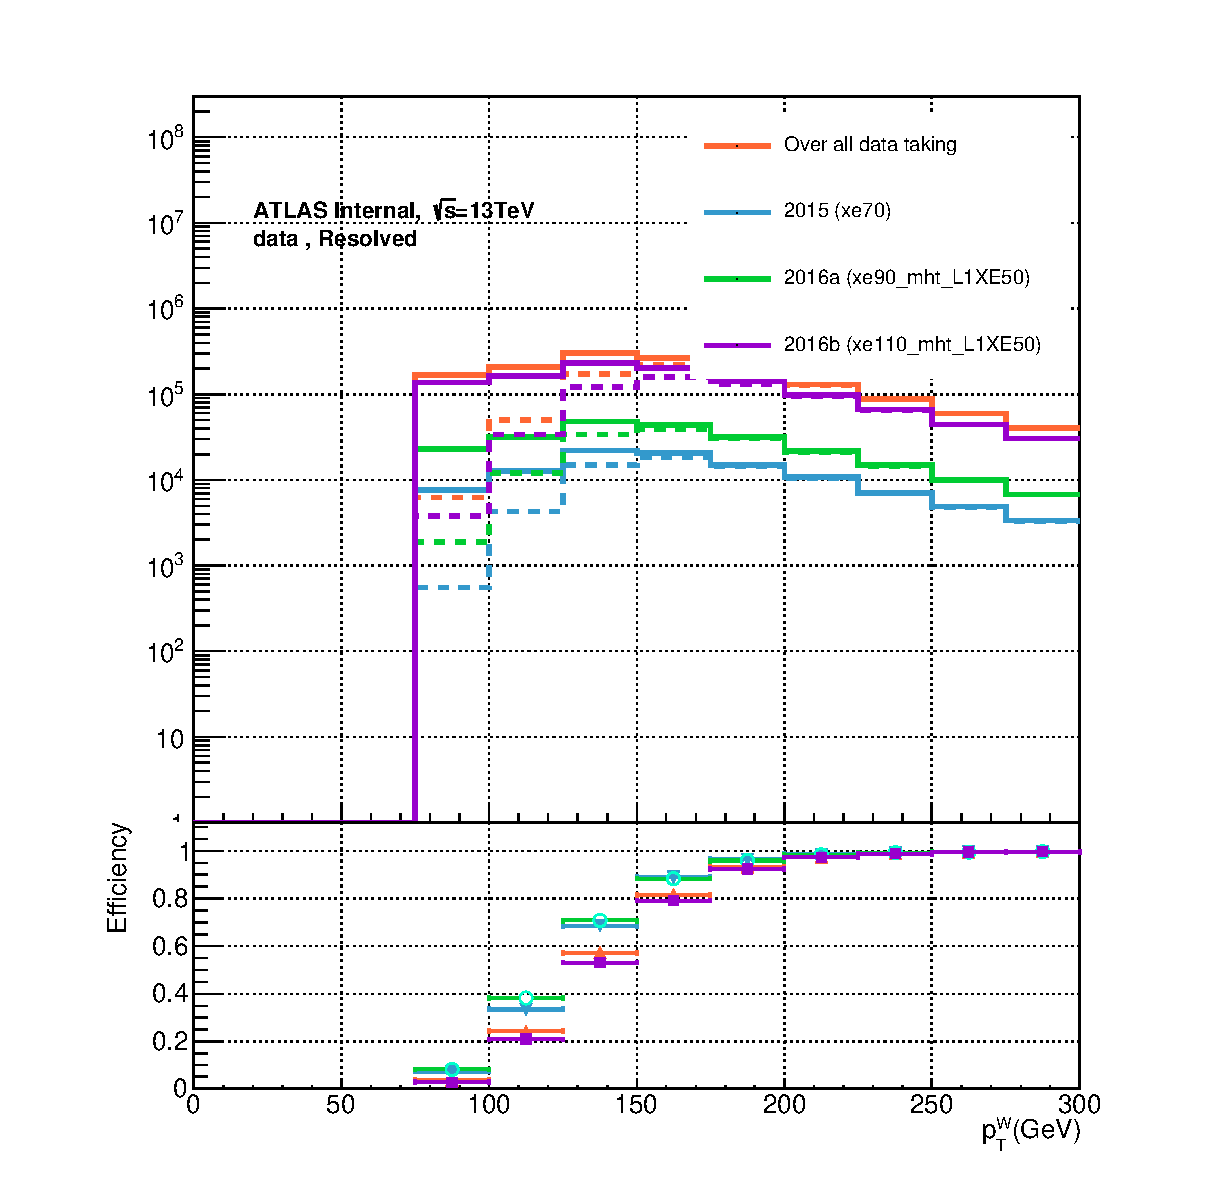
\includegraphics[width=0.4\hsize]{Chapter3/Resolved_TrigEff_ptW_METcut_data.eps}
		}
		\subfloat[]{
			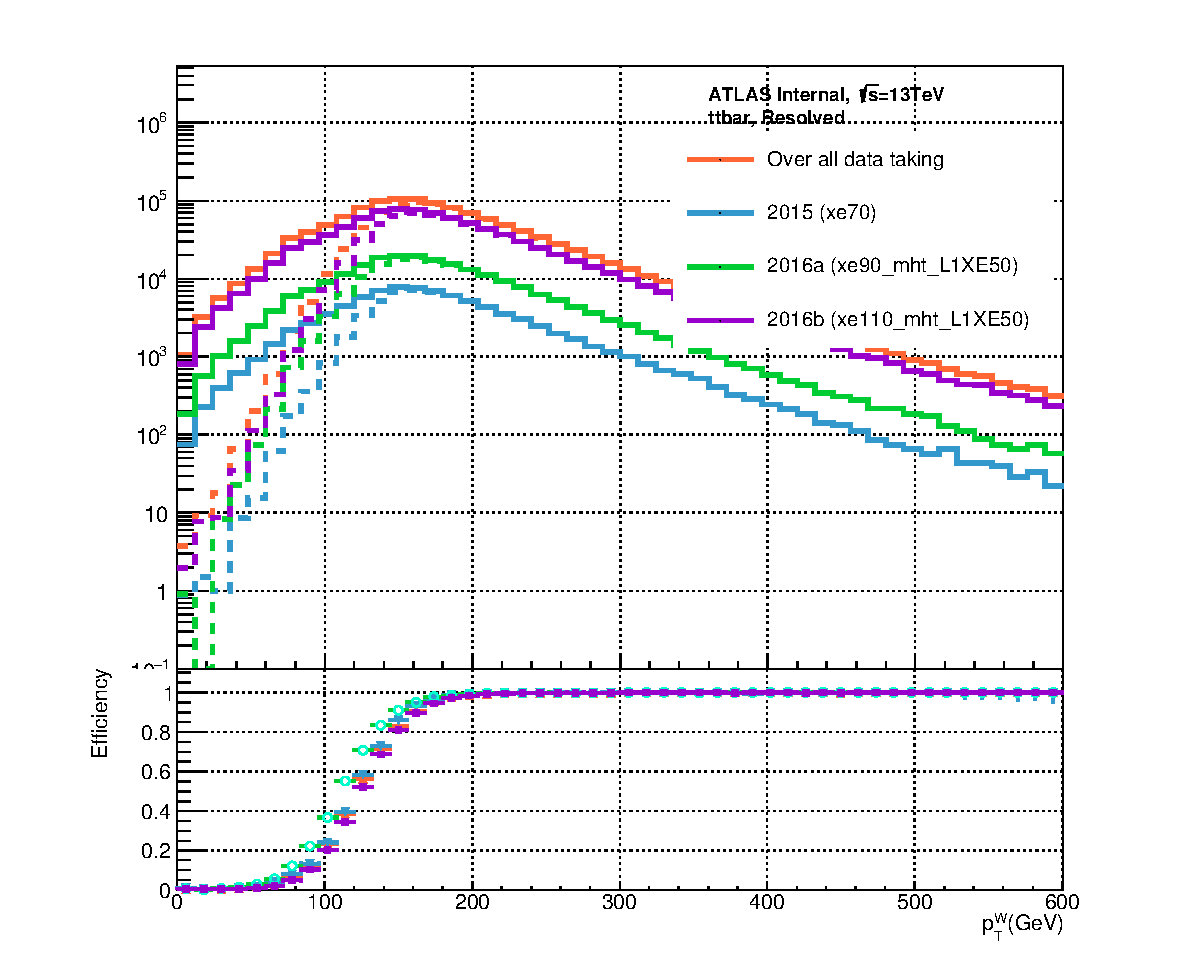
\includegraphics[width=0.48\hsize]{Chapter3/Resolved_TrigEff_ptW_METcut_ttbar-eps-converted-to}
		}
		\caption{The upper plot is $p_{T}(\mu\nu)$ distribution of tagged (real) and probed events in resolved channel for data (a) and $t\bar{t}$ events (b). The lower plots is the efficiency as a function of $p_{T}(\mu\nu)$}
		\label{Fig:eff_met_resolved}
	\end{center}
\end{figure}
\noindent
\subsection{Event Cleaning and Preselection}
After the trigger, the event ``quality is verified by a series of flags in data determining the suitability of an event for physical analyses. The following is the list:
\begin{itemize}
	\item {\bf Good Run}: if the detector operates in a proper status without intolerable defects, they go into the good run list (GRL). Only the events contained in the GRL are considered in this analysis. 
	\item {\bf Primary Vertex}: because all the physical objects are required to origin from the primary vertex, its existence is essential. Events without a proper primary vertex (defined in Sec. \ref{sec:obj rec}) are discarded.
	\item {\bf Tile Error Veto}: part of the channels in tile detector are broken. If they accept any physical objects, this flag would be marked, and the events are vetoed.
	\item {\bf LAr Error Veto}: part of the channels in LAr detector are broken. If they accept any physical objects, this flag would be marked, and the events are vetoed.
	\item {\bf SCT Error Veto}: part of the channels in SCT detector are broken. If they accept any physical objects, this flag would be marked, and the events are vetoed.
	\item {\bf Core Error Veto}: during data-taking periods, the atlas central DAQ system might suffer from some glitches which broke the data recording, and the flag is marked for events. They are also vetoed in this analysis. 
\end{itemize}
\subsection{Parameter of Interest, $m_{WV}$}
This analysis is searching for the mass resonance of exotic particles, so it is the discriminant to seek for the signal. (i.e. $m_WV$ distribution is the input for statistic interpretation.) However, the longitudinal $p_{T}$ of neutrinos in the final state could not be measured, so the mass resolution is poor to spot the signal spike. Therefore, $p_{z}(\nu)$ is solved with the assumption that $W\rightarrow l\nu$ is the $E^{miss}_{T}$ contribution in all the events although it is not held true in every event. Firstly, the equation of energy conservation of $W$ boson decay can be written down as:
\begin{equation}
m^2_W = m_{l}^{2} + 2E_{l}\sqrt{ p_{T,\nu}^2 + p_{z,\nu}^{2} }  - 2 \vec{p}_{{T},l} \cdot \vec{p}_{T, \nu} - 2 p_{z, l} p_{z,\nu}
\end{equation}
\noindent
In SM, W bosons have the mass of $80~GeV$, so $m_{l}$ for electrons and muons is negligible. This leads to the quadratic equation of $p_{z}^\nu$:
\begin{equation}
4p_{{T}, l}^{2} p_{z,\nu}^{2} - 4 \left( m_{W}^{2} + 2 \vec{p}_{{T}, l} \cdot \vec{p}_{{T},\nu} \right) p_{z,l} p_{z, \nu} - \left( m_{W}^{2} + 2\vec{p}_{{T}, l} \cdot \vec{p}_{{T},\nu}  \right)^{2} +4p_l^{2} p_{{T},\nu}^{2} = 0
\end{equation}
\noindent
If the solutions are complex, only the real terms are taken into this analysis, and the imaginary term is discarded. To determine which solution from the real terms to use, the resolution is compared with the absolute value of solutions (bigger one and smaller one) defined as:
\begin{equation}
\sigma = \frac{p_z^{truth}-p_z^{\nu}}{p_z^{truth}}
\end{equation}
\noindent
with $p_z^{truth}$ as the neutrino longitudinal momentum at generator level (MC truth). The result could be seen in Fig. \ref{Fig:netrinoPz}, and it indicates the bigger one has slightly better performance in terms of the mass resolution, so it is kept.  
\begin{figure}
	\centering
    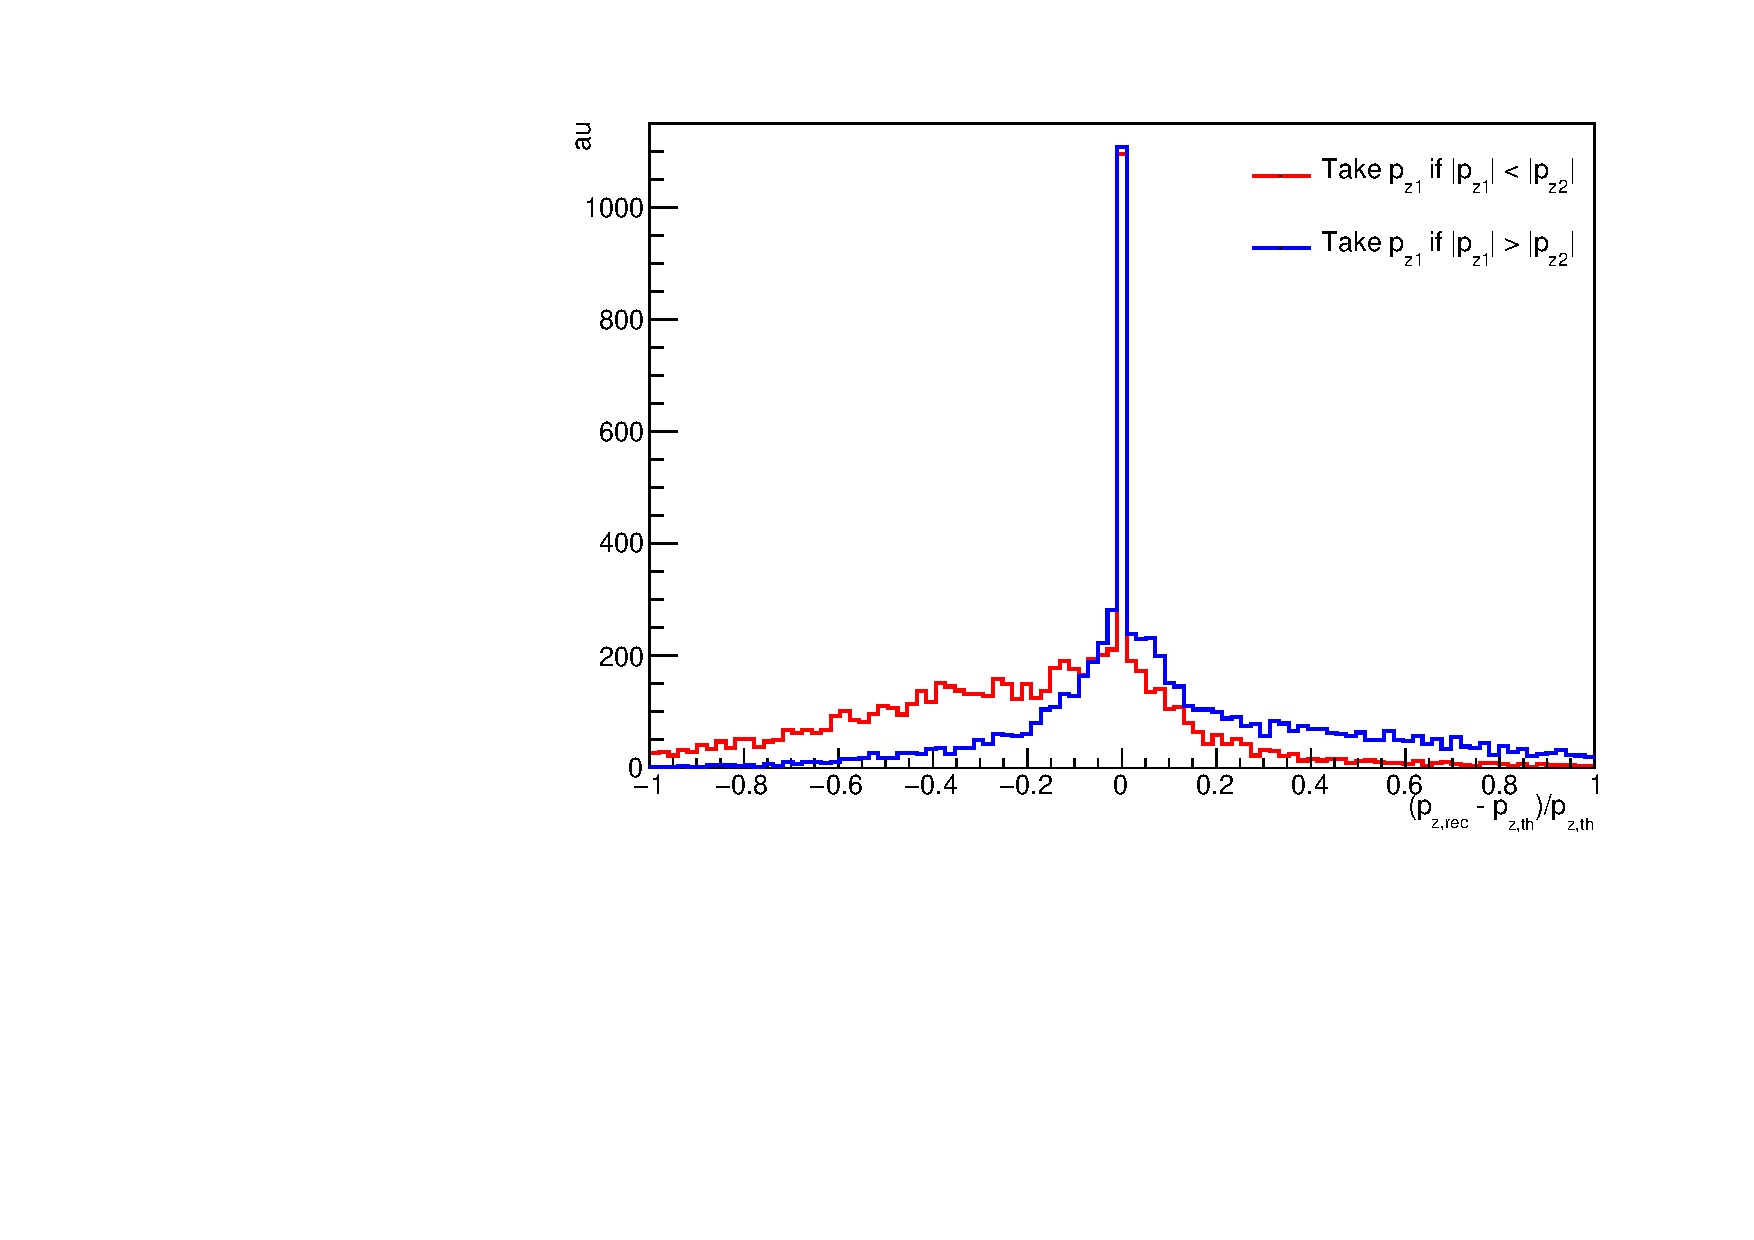
\includegraphics[width=0.5\hsize]{Chapter3/neutrinoPz}
    \caption{The $p_{z}^\nu$ resolution with absolute values of the solutions, bigger and smaller one. }
    \label{Fig:netrinoPz}
\end{figure}
\noindent
In addition to the correction on the leptonically decayed W boson, the other further improvement on $m_{WV}$ reconstruction is also made by $p_{T}(j,j)$ of the two resolved signal jets by the correction of $p_{T}^{corr}=p_{T}(j,j)\times \frac{m_{V}}{m_{jj}}$ (For WW, $m_V$ is taken as W boson mass, while it is Z boson mass for WZ medium state). The improvement of the ``mass-constraint'' correction could be seen in Fig. \ref{Fig:WHadmassConst} for $\approx 20\%$ better $m_{WV}$ resolution. 
\begin{figure}[h]
	\centering
	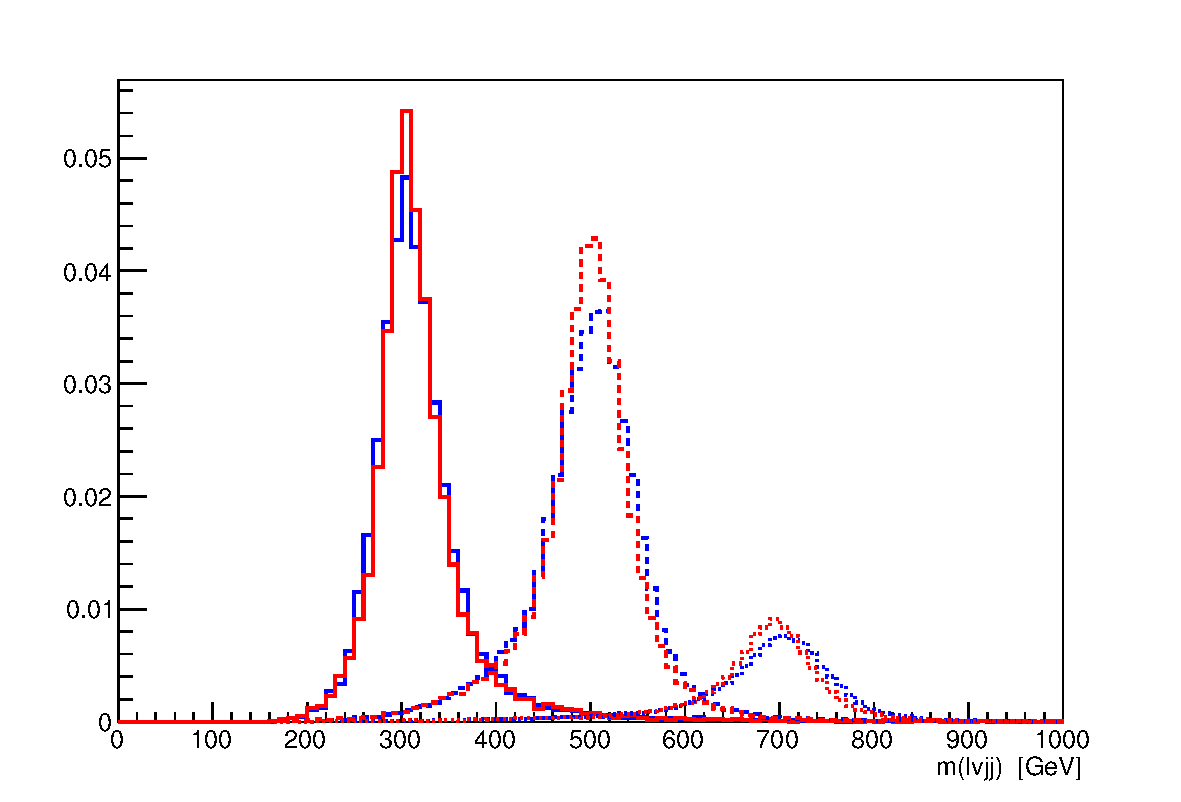
\includegraphics[width=0.6\hsize]{Chapter3/lvjjmass_WmassConstraint}
	\caption{$m_{WV}$ distributions for $gg \rightarrow H \rightarrow WW$ signals at $m=300GeV$ (solid), 500GeV (dashed) and 700GeV (dot), with (red) and without (blue) $W$-mass constraint to $W \rightarrow jj$ system.}\label{Fig:WHadmassConst}
\end{figure}
\noindent
\subsection{VBF Event Selection}
As VBF signal regions have better sensitivity than ggF/DY ones, the selection criteria play an important role in this analysis. The optimization on the selection is conducted in three steps. First, all VBF events are required to have at least 4(2) jets in the resolved (boosted) channel. Second, the the two jets in the dijet system are supposed to be the pair with the highest mass, opposite $\eta$ signs, and not b-tagged. This pair was chosen prior to the $W/Z\rightarrow jj$ signal jet selection and removed from signal jet candidates. Then, the optimization is performed on a 2-dimensional phase space constructed by $\Delta\eta(j,j)$ and $m(j,j)$ which are two most evident signatures of this production process. The performance of the cuts on the two variables is determined by signal significance in Eq. \ref{Eq:significance}. Fig. \ref{Fig:VBFOptimization} shows the result of the optimization performed on the signal sample with $700GeV$ HVT, and the best significance could be achieved by:
\begin{itemize}
	\item {\bf $m_{jj}^{VBF}> 770~GeV$}
	\item {\bf $\Delta\eta(jj)>4.7$}
\end{itemize}
The other reason to choose this set of cuts is to make it consistent with $WZ/ZZ \rightarrow lljj/\nu\nu jj$ analysis for the combination in next chapter. 
\begin{figure}[h]
	\centering
	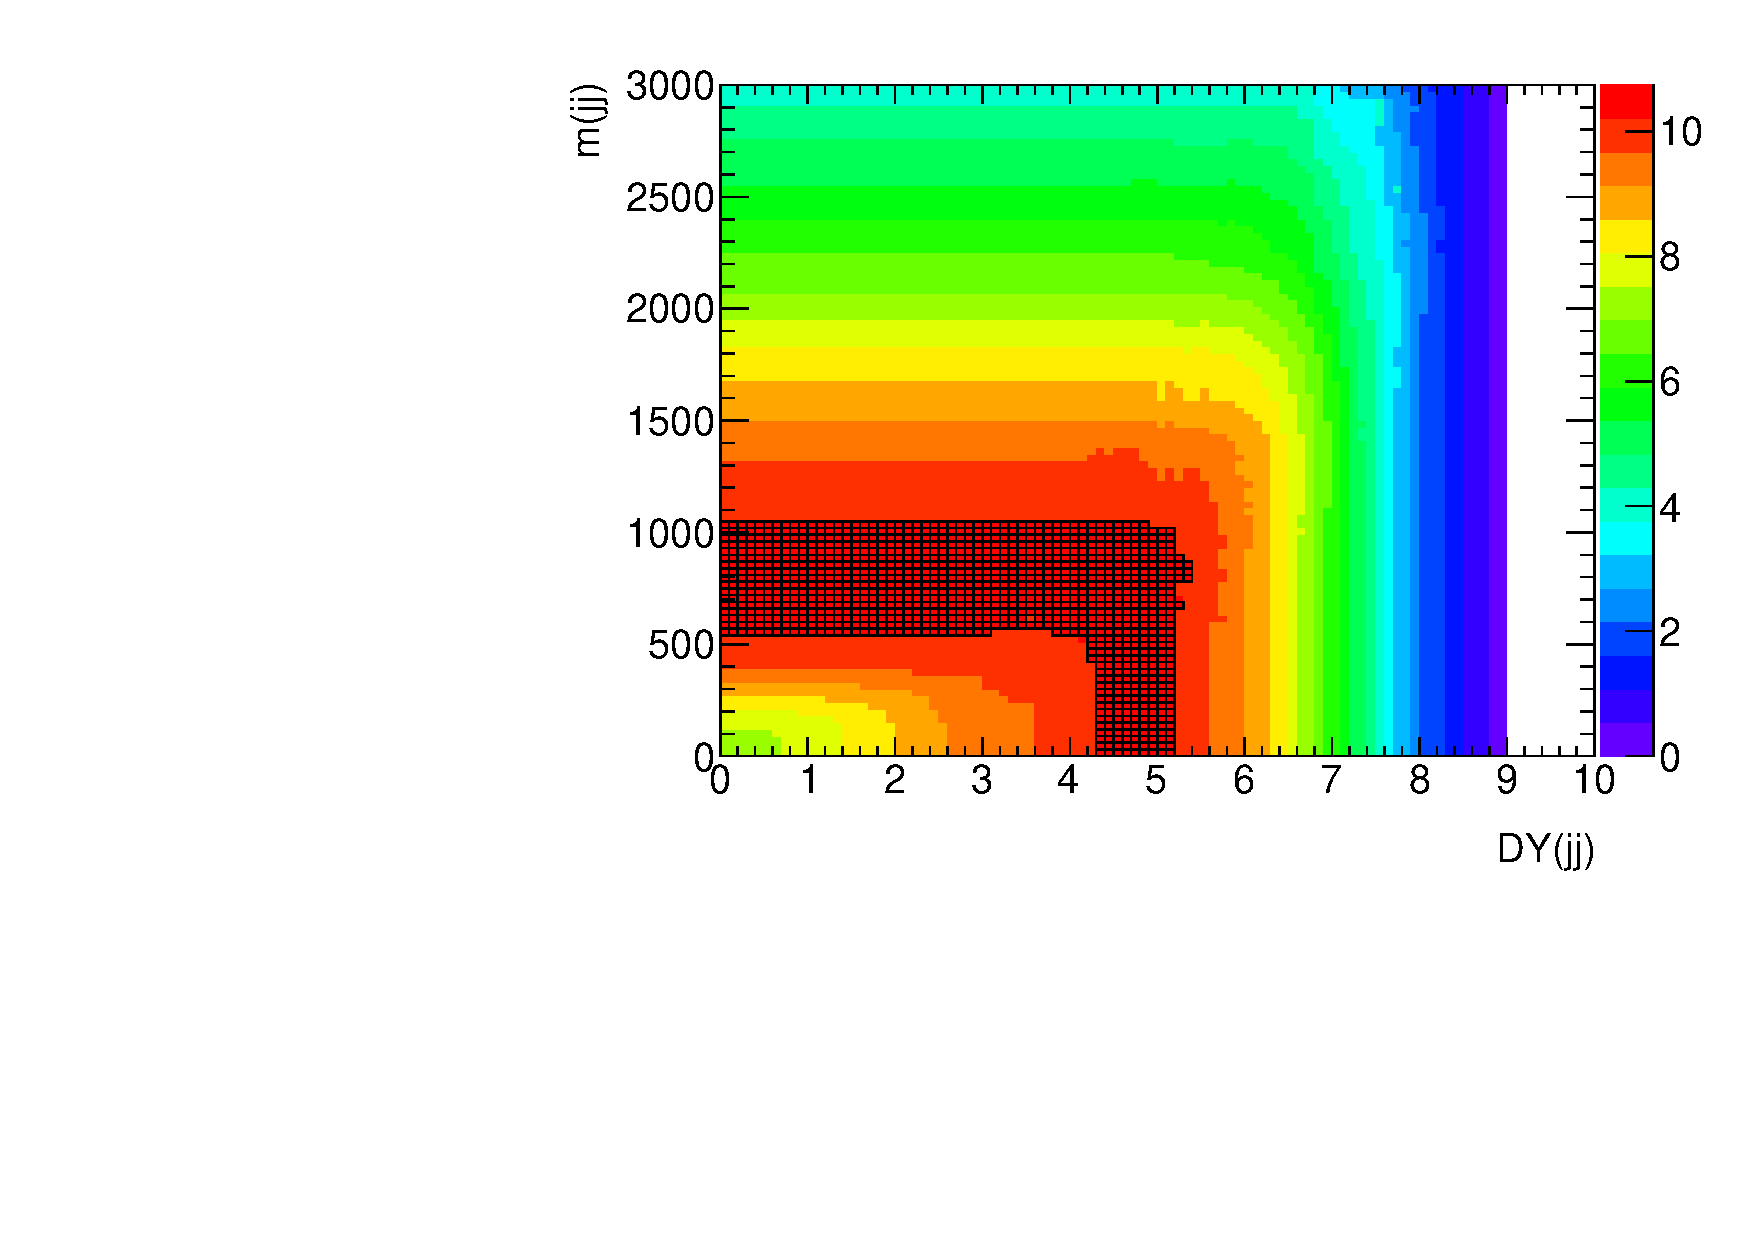
\includegraphics[width=0.7\textwidth]{Chapter3/VBF700_SignfSpace}
	\caption{The signal significance for the VBF $WW$ signal as a function of the VBF cuts $\Delta \eta(j_1,j_2)$ and $m(jj)$ for signal mass 700GeV (right). The black outlined bins are those whose values vary from the maximum by less than 5\%.}
	\label{Fig:VBFOptimization}
\end{figure}
\subsection{Boosted Event Selection}
In the boosted channel, the most important selection above the others is that at least one large R jet fulfils the W/Z boson $80\%$ efficiency working points. Then, those events are further categorized into high purity and low purity regions determined by whether the 50$\%$ working point is passsed. The full selection could be seen in Tab. \ref{tab:SRdefinitions}

\begin{table}[t]
	\caption{Summary of the selection criteria in the definition of the signal region (SR), $W$+jets control region ($W$ CR) and $t\bar{t}$ control region ($t\bar{t}$ CR), in the high-purity (HP) and low-purity (LP) categories.  } \label{tab:SRdefinitions}
	\begin{center}
		\begin{adjustbox}{center}
		\begin{tabular}{|l|l|c|c|c|c|c|c|}
			\hline
			\multicolumn{2}{|l|}{\multirow{2}{*}{Selection}} & \multicolumn{2}{c|}{SR}  &  \multicolumn{2}{c|}{$W$ CR}  & \multicolumn{2}{c|}{$t\bar{t}$ CR} \\
			\cline{3-8}
			\multicolumn{2}{|l|}{} & HP & LP &HP & LP & HP & LP \\
			\hline
			\multirow{4}{*}{$W\rightarrow l\nu$} & Num of signal leptons & \multicolumn{6}{c|}{ 1 } \\
			\cline{2-8}
			&Num of vetoed leptons & \multicolumn{6}{c|}{ 0 }  \\
			\cline{2-8}
			&\vphantom{\Large B} $E^{miss}_{T}$ & \multicolumn{6}{c|}{ $>100GeV$ } \\
			\cline{2-8}
			&$p_{T}(l\nu)$ & \multicolumn{6}{c|}{ $>200GeV$ } \\
			\hline
			\multirow{5}{*}{$W/Z\rightarrow J$} & Num of large-$R$ jets & \multicolumn{6}{c|}{ $\geq 1$ } \\
			\cline{2-8}
			& \vphantom{\Large B} $D^{(\beta=1)}_2$ 50\,\% WP & pass & fail & pass & fail & pass & fail \\
			\cline{2-8}
			& \vphantom{\Large B} $D^{(\beta=1)}_2$ 80\,\% WP & --- & pass  & --- & pass  & --- & pass \\
			\cline{2-8}
			& $W/Z$ mass 50\,\% WP & pass &fail& --- & --- & pass & fail\\
			\cline{2-8}
			& $W/Z$ mass 80\,\% WP &  --- & pass & fail & fail & --- & pass\\
			\hline
			\multirow{2}{*}{Topology cuts}
			& $p_{T}(l\nu) / m_{WV}$ & \multicolumn{6}{c|}{ \multirow{2}{*}{$>0.3 (0.4)$ for VBF (ggF) category } }\\
			& $p_{T}(J) / m_{WV}$  & \multicolumn{6}{c|}{} \\
			\hline
			Top-quark veto & Num of $b$-tagged jets & \multicolumn{4}{c|}{0} & \multicolumn{2}{c|} {$\geq 1$} \\
			\hline
			Multi-jet BG Cleaning Cut & $E_T^{miss} / p_T(lv) > 0.2$ & \multicolumn{6}{c|}{ Electron channel only } \\
			\hline
			\multicolumn{2}{|c|}{Existence of VBF jets} & \multicolumn{6}{c|}{ yes (no) for VBF (ggF) category } \\
			\hline
		\end{tabular}
	    \end{adjustbox}
	\end{center}
\end{table}
\noindent
\\For the leptonically decayed system, the requirement is that exactly one signal is selected with $E^{miss}_{T}$ above $100GeV$ to suppress the multijet background. The additional requirements on the system is two topological cuts on kinetic properties: 
\begin{itemize}
	\item (a) $E^{miss}_{T}/p_{T}(e,\nu)>0.2$
	\item (b) $p_{T}(e,\nu)>0.2/m{WV}>0.3(0.4)$ for VBF (ggF) category
\end{itemize}
(a) is only for the electron channel to reduced multijet background further in the concern of the jet-faked electrons, while (b) is to lower the SM background contribution for the energy balance between the leptonically and hadronically decayed systems. These criteria are consistent across signal and control regions. 
\\
\\In the side of the hadronically decayed boson is only the large R jet. In addition to the requirement in the last section, the high purity regions (HP) (for both signal and control regions) demand the fat jet boson-tagged at $50\%$ WP, and it is the most sensitive region to signal. For the events with fat jets failing $50\%$ but passing $80\%$ WPs, they went into the low purity region (LP), and the combined sensitivity of HP and LP signal regions could be improved by around $~10\%$. If the fat jet only fails mass cut and pass the $D_{2}^{\beta=1}$ of boson tagging, this event would not be discarded but be chosen into W+jet control region instead. Finally, $p_{T}$ of the fat jet is also required to be above $0.3(0.4)m_{WV}$ for the energy balance in VBF(ggF) category. The event categorization of signal and W+jet control regions for both high and low purity categories is illustrated in Fig. \ref{Fig:HPLPdefinitions}.
\begin{figure}[h]
	\centering
	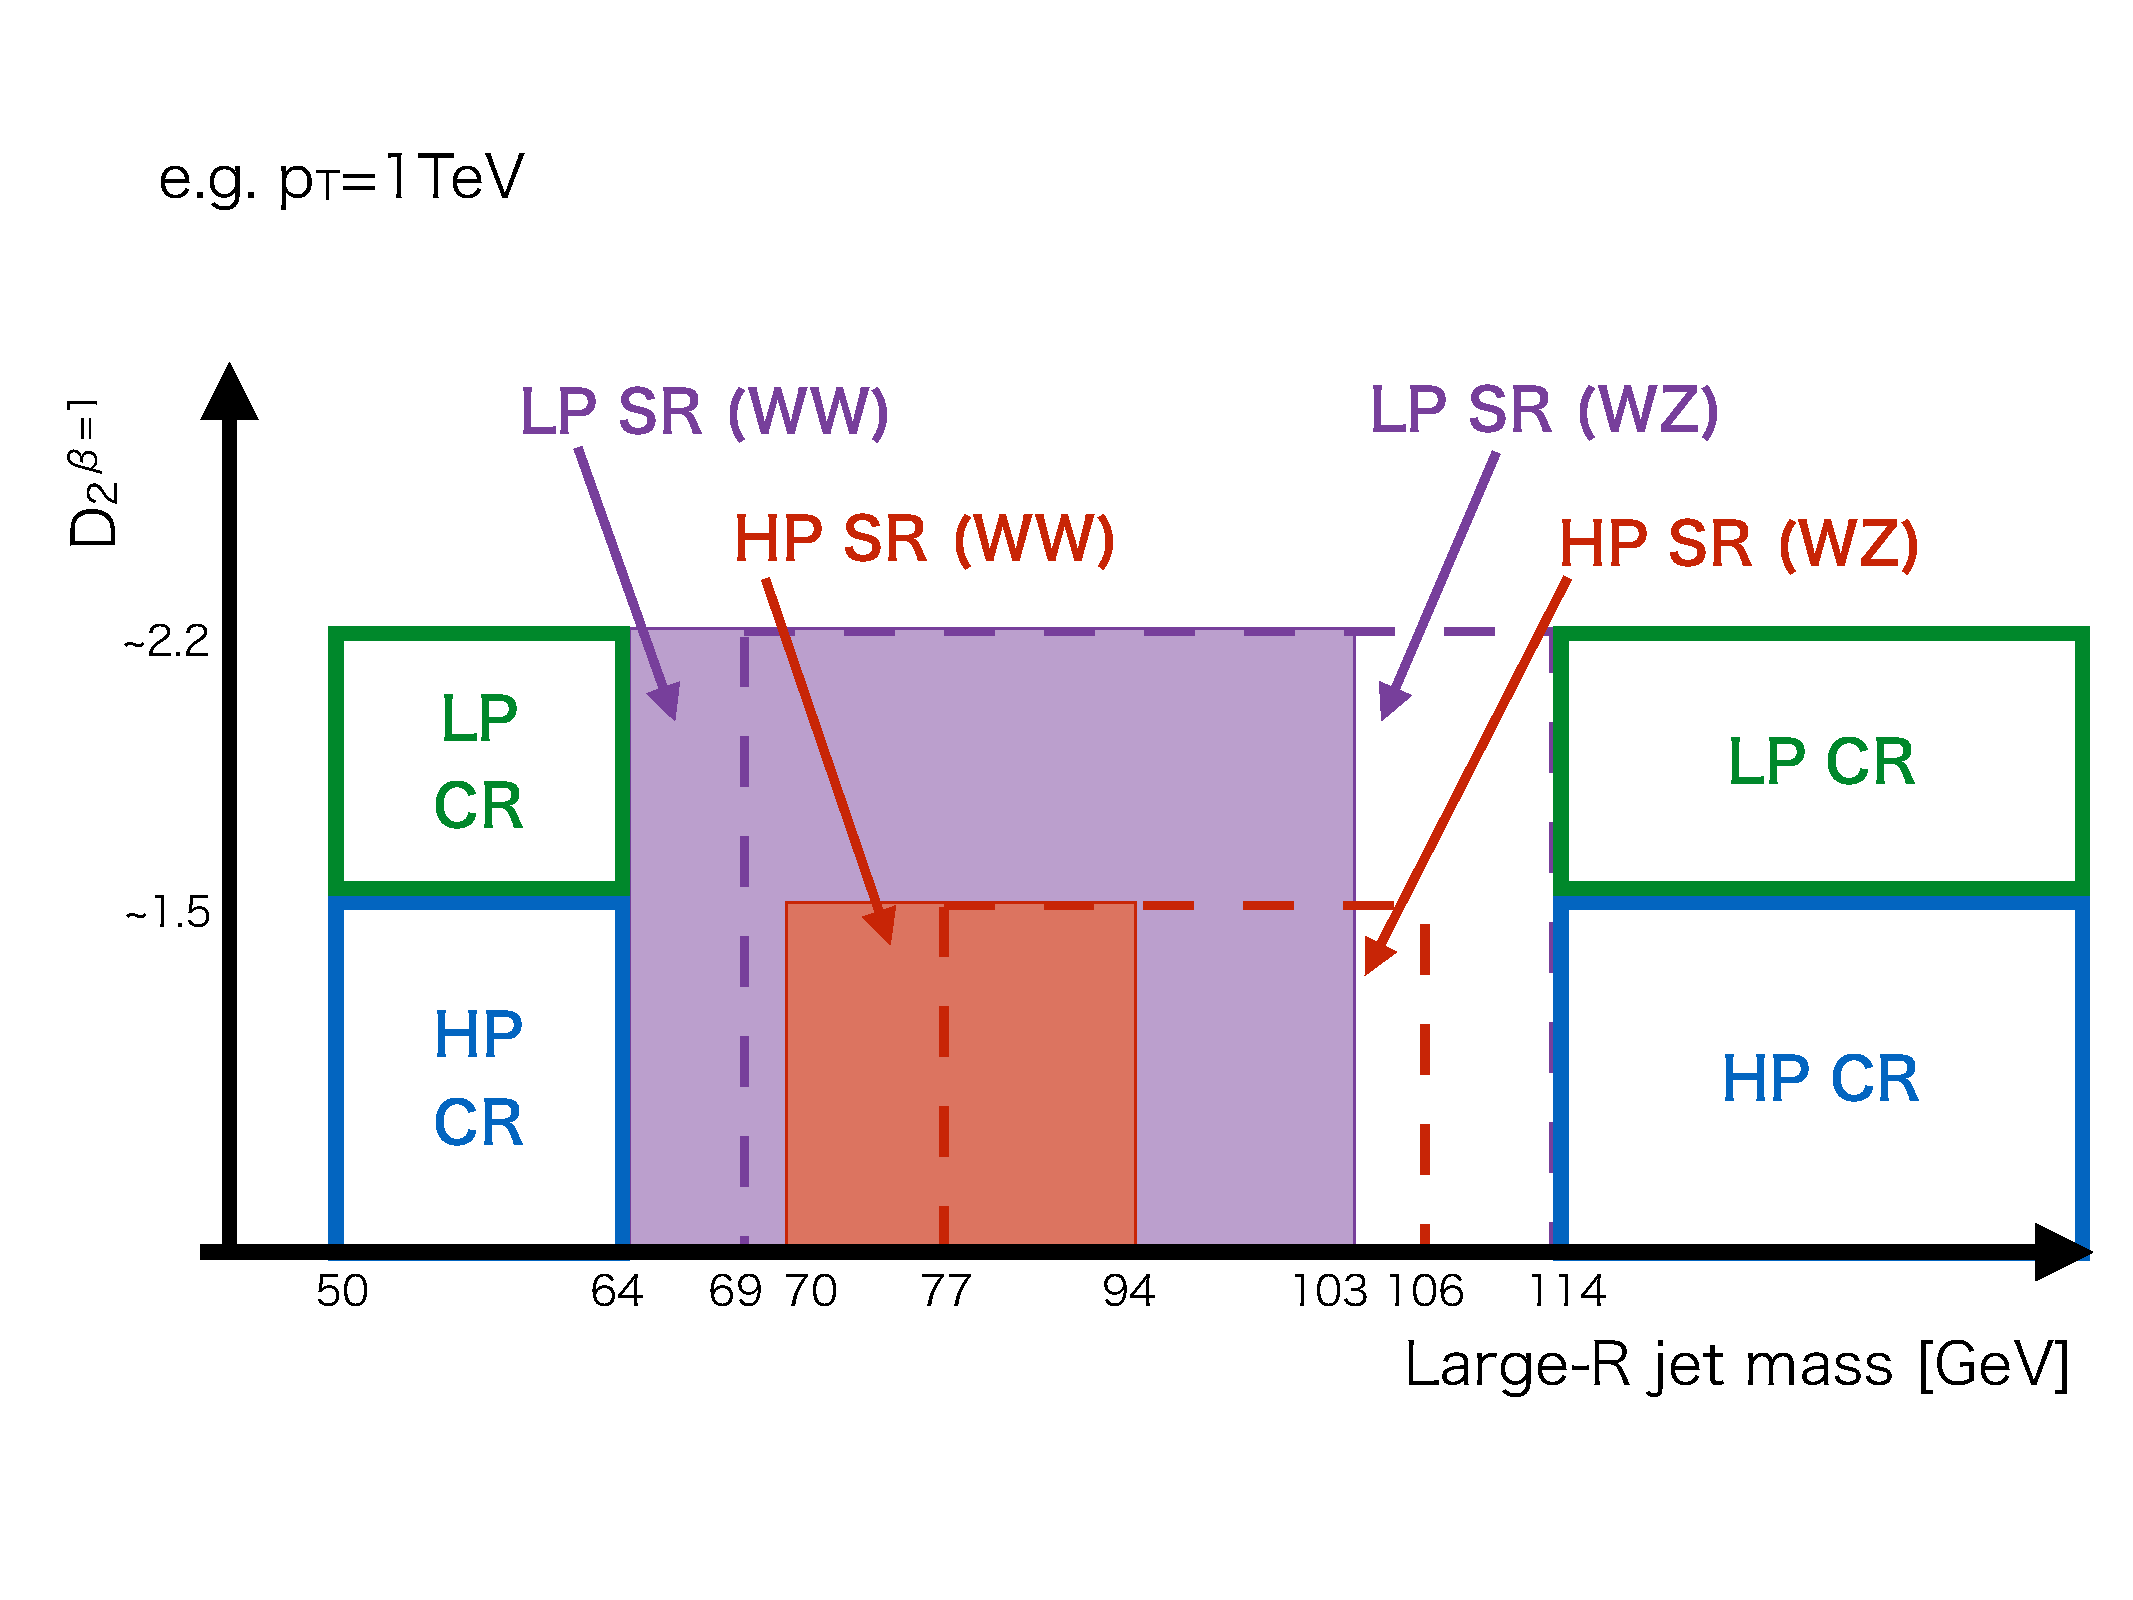
\includegraphics[width=0.8\hsize]{Chapter3/HPLPdefinitions}
	\caption{Definitions of signal region (SR) and $W$+jets control region (WR) for the event with the large-R jet of $\pt=1\,\TeV$ based on fat jet boson tagging and number of b-tagged jets }
	\label{Fig:HPLPdefinitions}
\end{figure}
\noindent
To reduce the $t\bar{t}$ background contribution, the subjets associated to the selected large R jet shall not be b-tagged in the W+jet control region and signal region. If any of them or the small R jets ($R=0.4$) pass the $85\%$ b-tagging WP, the event would go into the top control region. 
\\
\\Fig. \ref{Fig:HighPuritySR} and Fig. \ref{Fig:LowPuritySR} are the $m_{WV}$ distributions for the comparison of signal and background events in high purity and low purity signal regions for electron and muon channels respectively. 
\begin{figure}[h]
	\begin{center}
		\subfloat[]{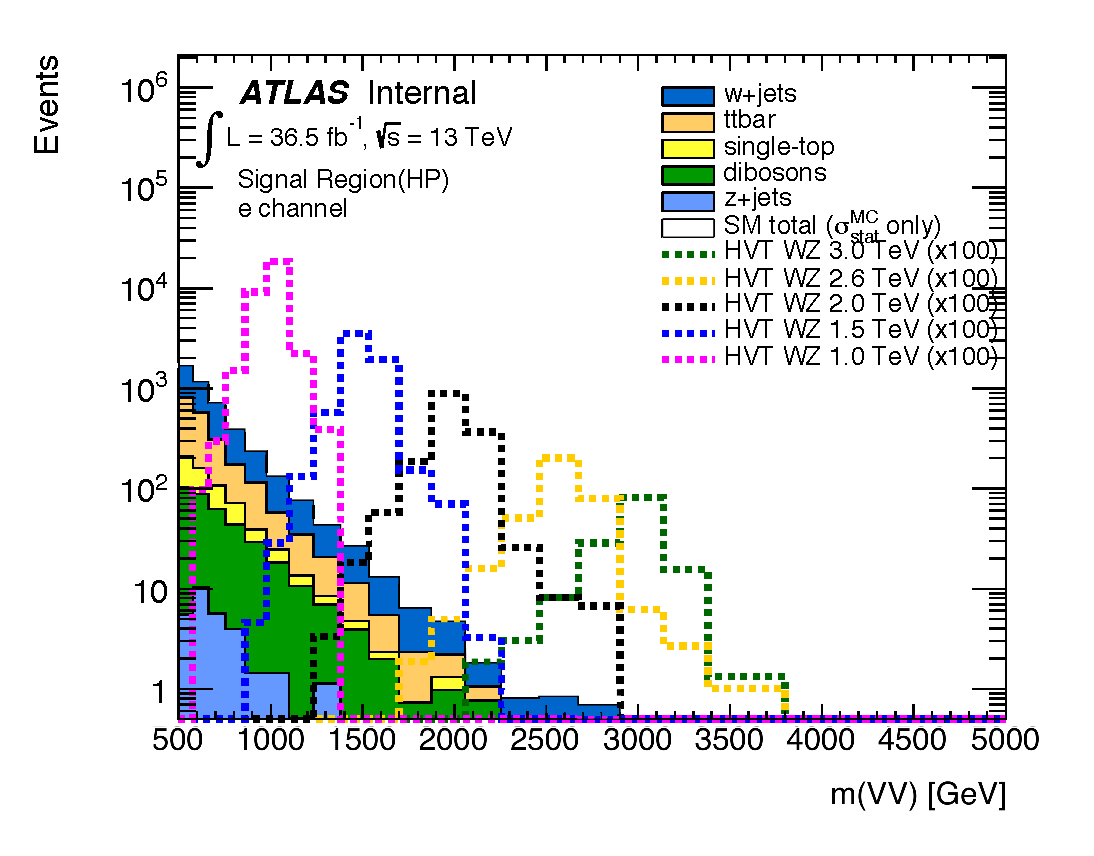
\includegraphics[width=0.5\hsize]{Chapter3/lvJmass_bveto_e.eps}}
		\subfloat[]{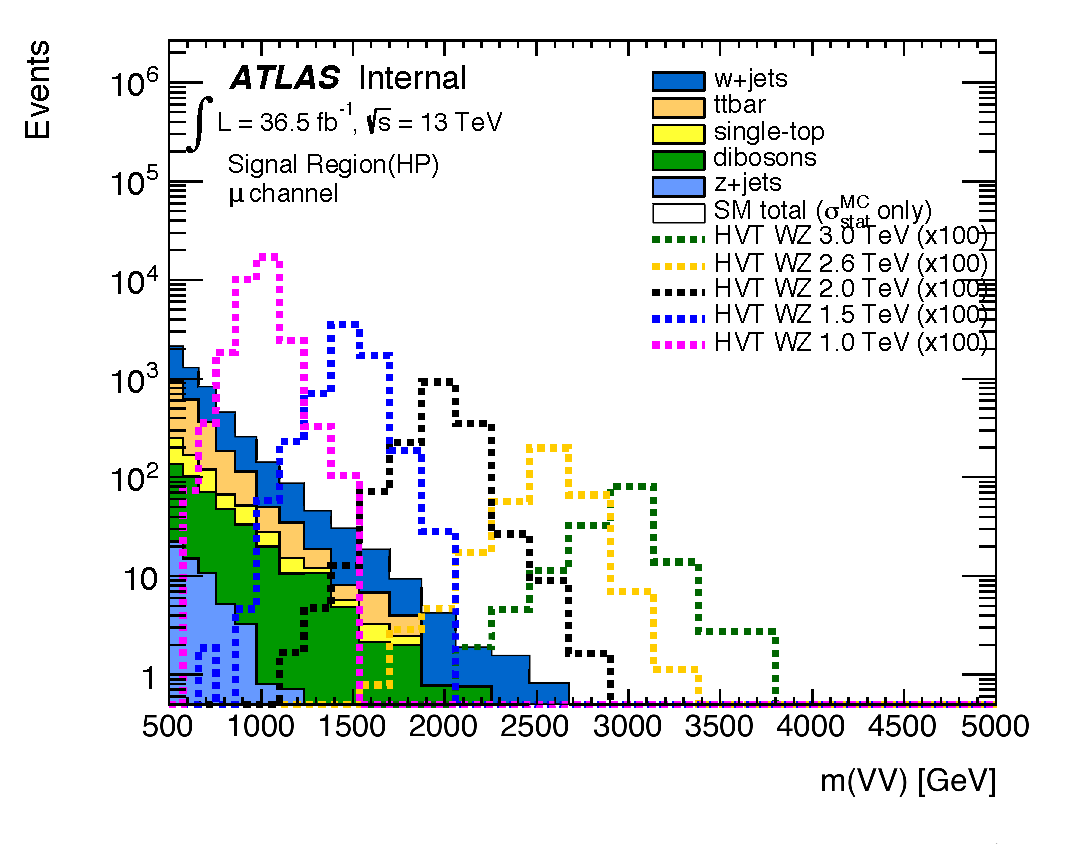
\includegraphics[width=0.5\hsize]{Chapter3/lvJmass_bveto_mu.eps}}
	\end{center}
	\caption{The $m_{WV}$ distributions in the HP signal region for (a) electron and (b) muon channel, with the integrated luminosity of $36.5~fb^{-1}$. The HVT $WZ$ signals with $m=1.0TeV$, $1.5TeV$, $2.0TeV$, $2.6TeV$ and $3.0TeV$ are overlaid scaled to $100 ~\times$ cross section}
	\label{Fig:HighPuritySR}
\end{figure}

\begin{figure}[h]
	\centering
	\subfloat[]{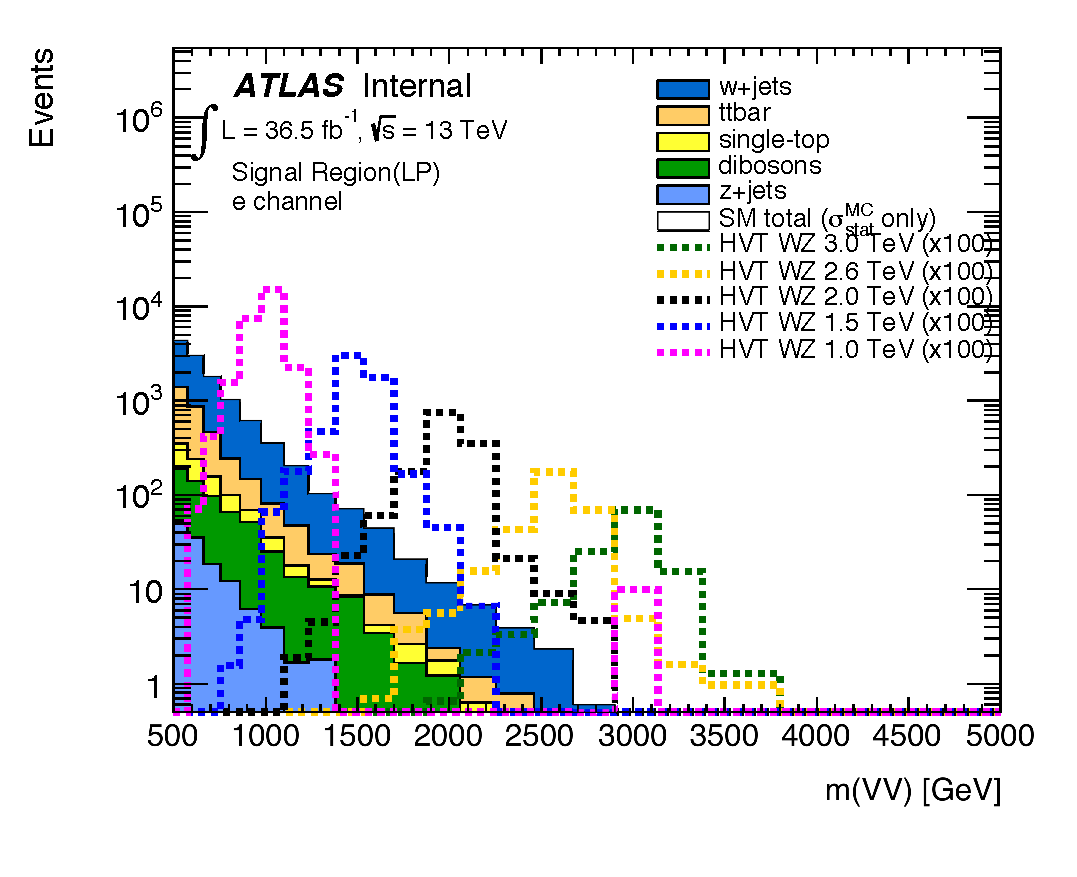
\includegraphics[width=0.5\hsize]{Chapter3/lvJmass_lowPurity_e.eps}}
	\subfloat[]{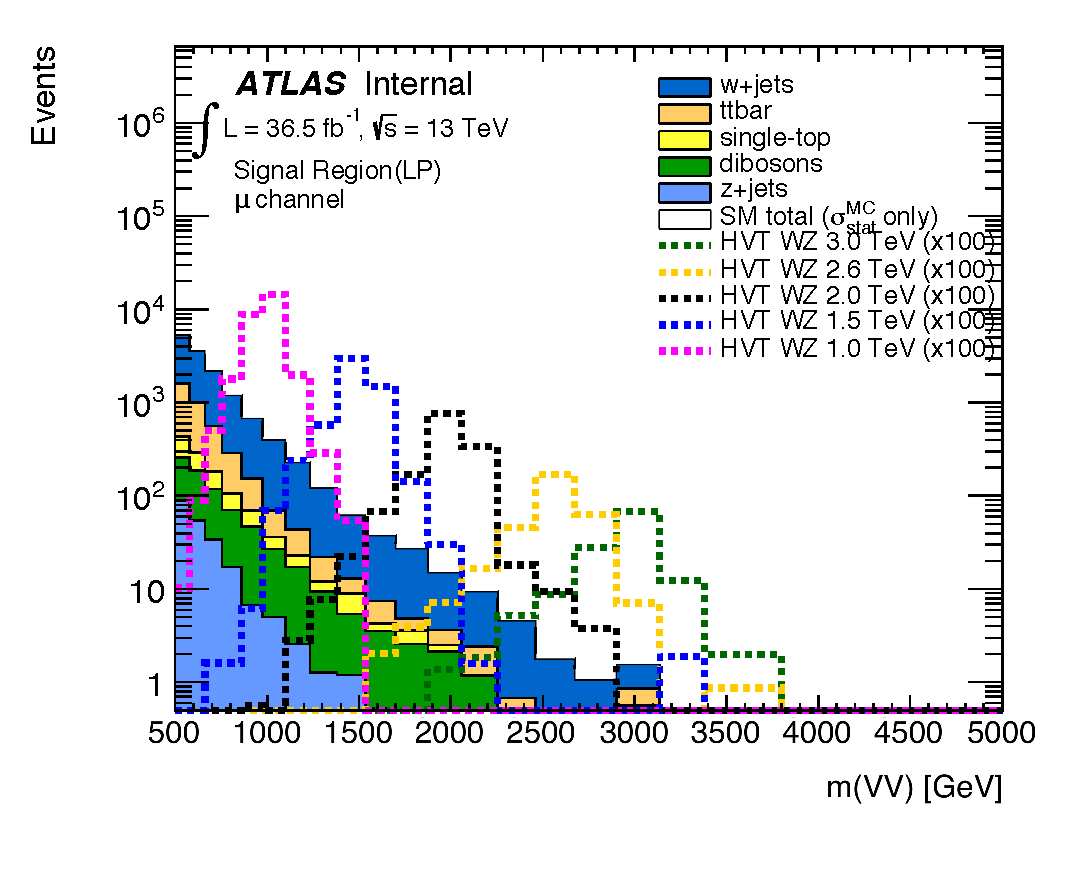
\includegraphics[width=0.5\hsize]{Chapter3/lvJmass_lowPurity_mu.eps}}
	\caption{The $m_{WV}$ distribution in the LP signal region for (a) electron and (b) muon channel, with the integrated luminosity of $36.5~fb^{-1}$.The HVT $WZ$ signals with $m=1.0TeV$, $1.5TeV$, $2.0TeV$, $2.6TeV$ and $3.0TeV$ are overlaid 
	scaled to $100 ~\times$ cross section.}
	\label{Fig:LowPuritySR}
\end{figure}
%

\subsection{Resolved Event Selection}
The resolved channel has a lower sensitivity than the boosted channel, but it still helps to recover the lost events in the lower energy regime. If the event has no fat jet fulfilling the selection criteria, it went to the resolved category. The full selection for both resolved signal and control regions could be seen in Tab. \ref{Tab:SRdefinitions_resolved}
\begin{table}[t]
	\caption{Summary of the selection criteria of of the  the resolved analysis for the $WW$ and $WZ$ signal regions (SR), $W$+jets control region (WR) and $ t\bar{t}$ control region (TR). } \label{Tab:SRdefinitions_resolved}
	\begin{center}
		\resizebox{\textwidth}{!}{
			\begin{tabular}{|l|l|c|c|c|c|}
				\hline
				\multicolumn{2}{|l|}{cuts} & $WW$ SR & $WZ$ SR & WR & TR \\
				\hline
				\multirow{3}{*}{$W\rightarrow \ell\nu$ selection} & Number of signal leptons & \multicolumn{4}{c|}{ 1 } \\
				\cline{2-6}
				&Number of veto leptons & \multicolumn{4}{c|}{ 0 }  \\
				\cline{2-6}
				&$E^{miss}_{T}$ & \multicolumn{4}{c|}{ $>60GeV$ } \\
				\cline{2-6}
				&$\pt(\ell\nu)$ & \multicolumn{4}{c|}{ $>75GeV$ } \\
				\hline
				\multirow{4}{*}{$W/Z\rightarrow jj$ selection} & Number of small jets & \multicolumn{4}{c|}{ $\geq2$ } \\ %$\geq 2$ & $\geq 2$ & $\geq 2$  \\
				\cline{2-6}
				& $\pt (j1)$ & \multicolumn{4}{c|}{ $>60$~GeV}\\
				\cline{2-6}
				& $\pt (j2)$ & \multicolumn{4}{c|}{ $>45$~GeV}\\
				\cline{2-6}
				& $m_{jj}$ & [66, 94]GeV\ & [82, 106]GeV\ & $<66GeV$ &  [66, 106]GeV \\
				&  &  &  & or [106, 200]GeV & \\
				\hline
				\multirow{6}{*}{Topology cuts} & $\Delta\phi(j,\ell)$ & \multicolumn{4}{c|}{ $>1.0$}\\
				\cline{2-6}
				& $\Delta\phi(j,E^{miss}_{T})$ & \multicolumn{4}{c|}{ $>1.0$}\\
				\cline{2-6}
				& $\Delta\phi(j,j)$ & \multicolumn{4}{c|}{ $<1.5$}\\
				\cline{2-6}
				& $\Delta\phi(l,E^{miss}_{T})$ & \multicolumn{4}{c|}{ $<1.5$}\\
				\cline{2-6}
				& $\pt(e\nu) / m_{WV}$ &\multicolumn{4}{c|}{\multirow{2}{*}{$>0.3 (0.35)$ for VBF (ggF) category}}\\
				& $\pt(jj) / m_{WV}$ & \multicolumn{4}{c|}{ } \\
				\hline
				\multirow{2}{*}{Top veto} & Number of $b$-tagged jets in $W/Z$ & $\leq 1$ & $\leq 2$ & $\leq 1$ & $\geq2$ \\
				\cline{2-6}
				& Number of other $b$-tagged jets & \multicolumn{3}{c|}{0} & or $\geq 1$ \\
				\hline
				\multicolumn{2}{|c|}{Existence of VBF jets} & \multicolumn{4}{c|}{ yes (no) for VBF (ggF) category } \\
				\hline
			\end{tabular}
		}
	\end{center}
\end{table}

As in the boosted channel, the system of leptonically decayed W boson has a signal lepton fulfilling the object definition of the last section. However, the $E_{T}^{miss}$ cut here is lowered to $60~GeV$ for the less energetic system as compared to the boosted channel. For the energy balance, the ratio between $p_{T}(l,\nu)$ and $m_{WV}$ shall be be over 0.3 (0.35) for VBF (ggF) category. 
\\
\\In the hadronic side, the two signal jets are selected after VBF jets, and they are required to have $p_{T}$ above $60~GeV$ ($45~GeV$) for the leading (subleading) one to suppress the SM background. As they are decayed from W or Z boson, their combined mass shall be within the dedicated mass windows, which are $[66, 94]~GeV$ for the WW signal region and $[82, 106]~GeV$ for the WZ signal region. Because the same top control region is used to make constraint in both of the two signal regions, the mass window is set at $[66,106]~GeV$ as the OR condition of W and Z mass windows. Events with a dijet mass which falls into the side band region ($[0,66]~GeV$ or $[106,200]~GeV$) are taken into the W+jet control region. The energy balance requirement here is the same as the leptonic system: $p_{T}(jj)/m_{WV}>0.3(0.35)$ for the VBF (ggF) category. The two selected jets in the W(Z) mass window are allowed to have one(two) of them b-tagged. The existence of any additional b-tagged jets would then make the event go into the top control region.  
\\
\\Different from the boosted channel, the resolved channel has the abundant background contribution from multijet events (details in next section), so a series of topological cuts are applied on the signature topology to further suppress with the optimization by the study on the dijet MC samples, which are listed below:
\begin{itemize}
	\item $\Delta\phi(j,l)>1.0$
	\item $\Delta\phi(j,E^{miss}_{T})>1.0$
	\item $\Delta\phi(j,j)<1.5$
	\item $\Delta\phi(l,E^{T}_{miss})<1.5$
\end{itemize}
\noindent
\\Fig. \ref{Fig:ResolvedSR} is the $m_{WV}$ distributions for comparison of signal and background in resolved signal regions for ggF and VBF categories respectively. The signal samples are with lower mass, because resolved channel has better sensitivity to them. 
\begin{figure}[h]
	\centering
	\subfloat[]{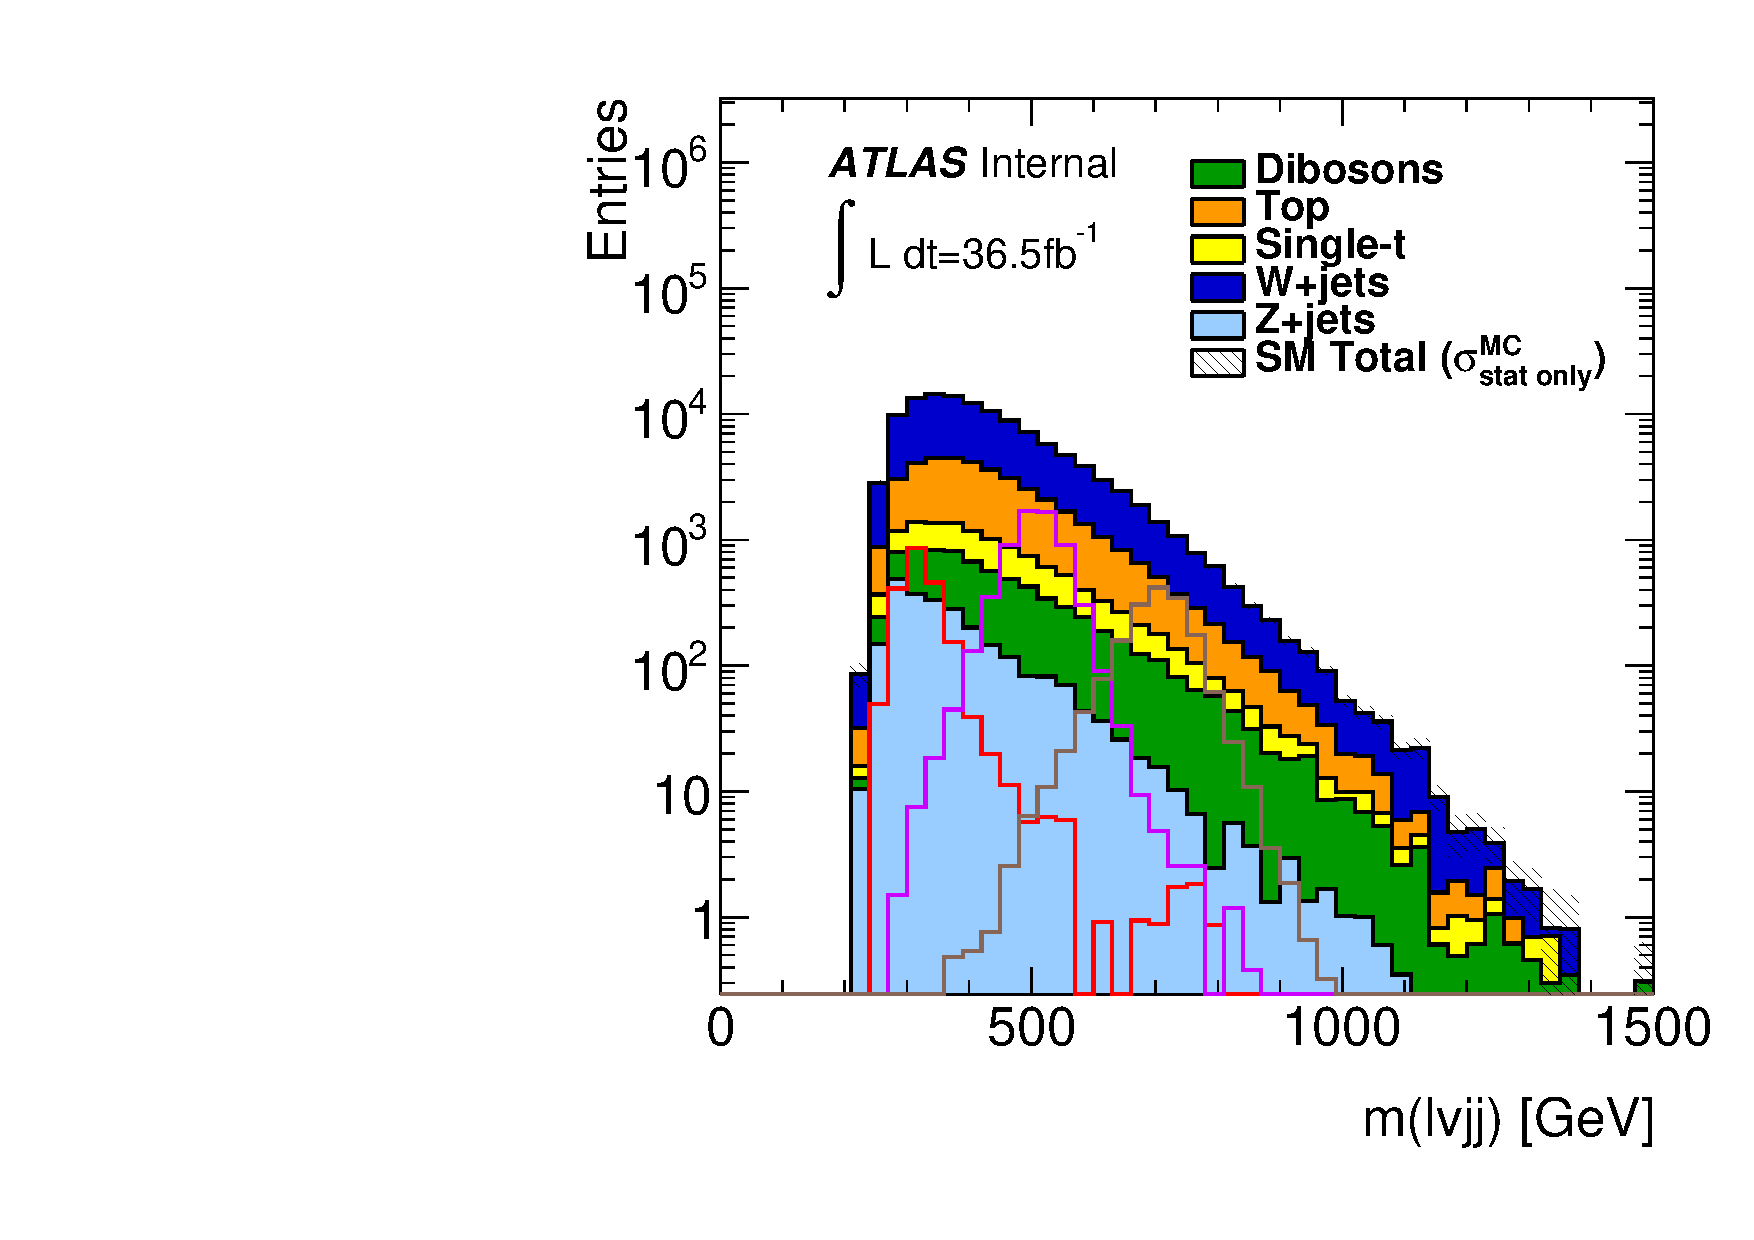
\includegraphics[width=0.5\hsize]{Chapter3/lvjjmass_ggF}}
	\subfloat[]{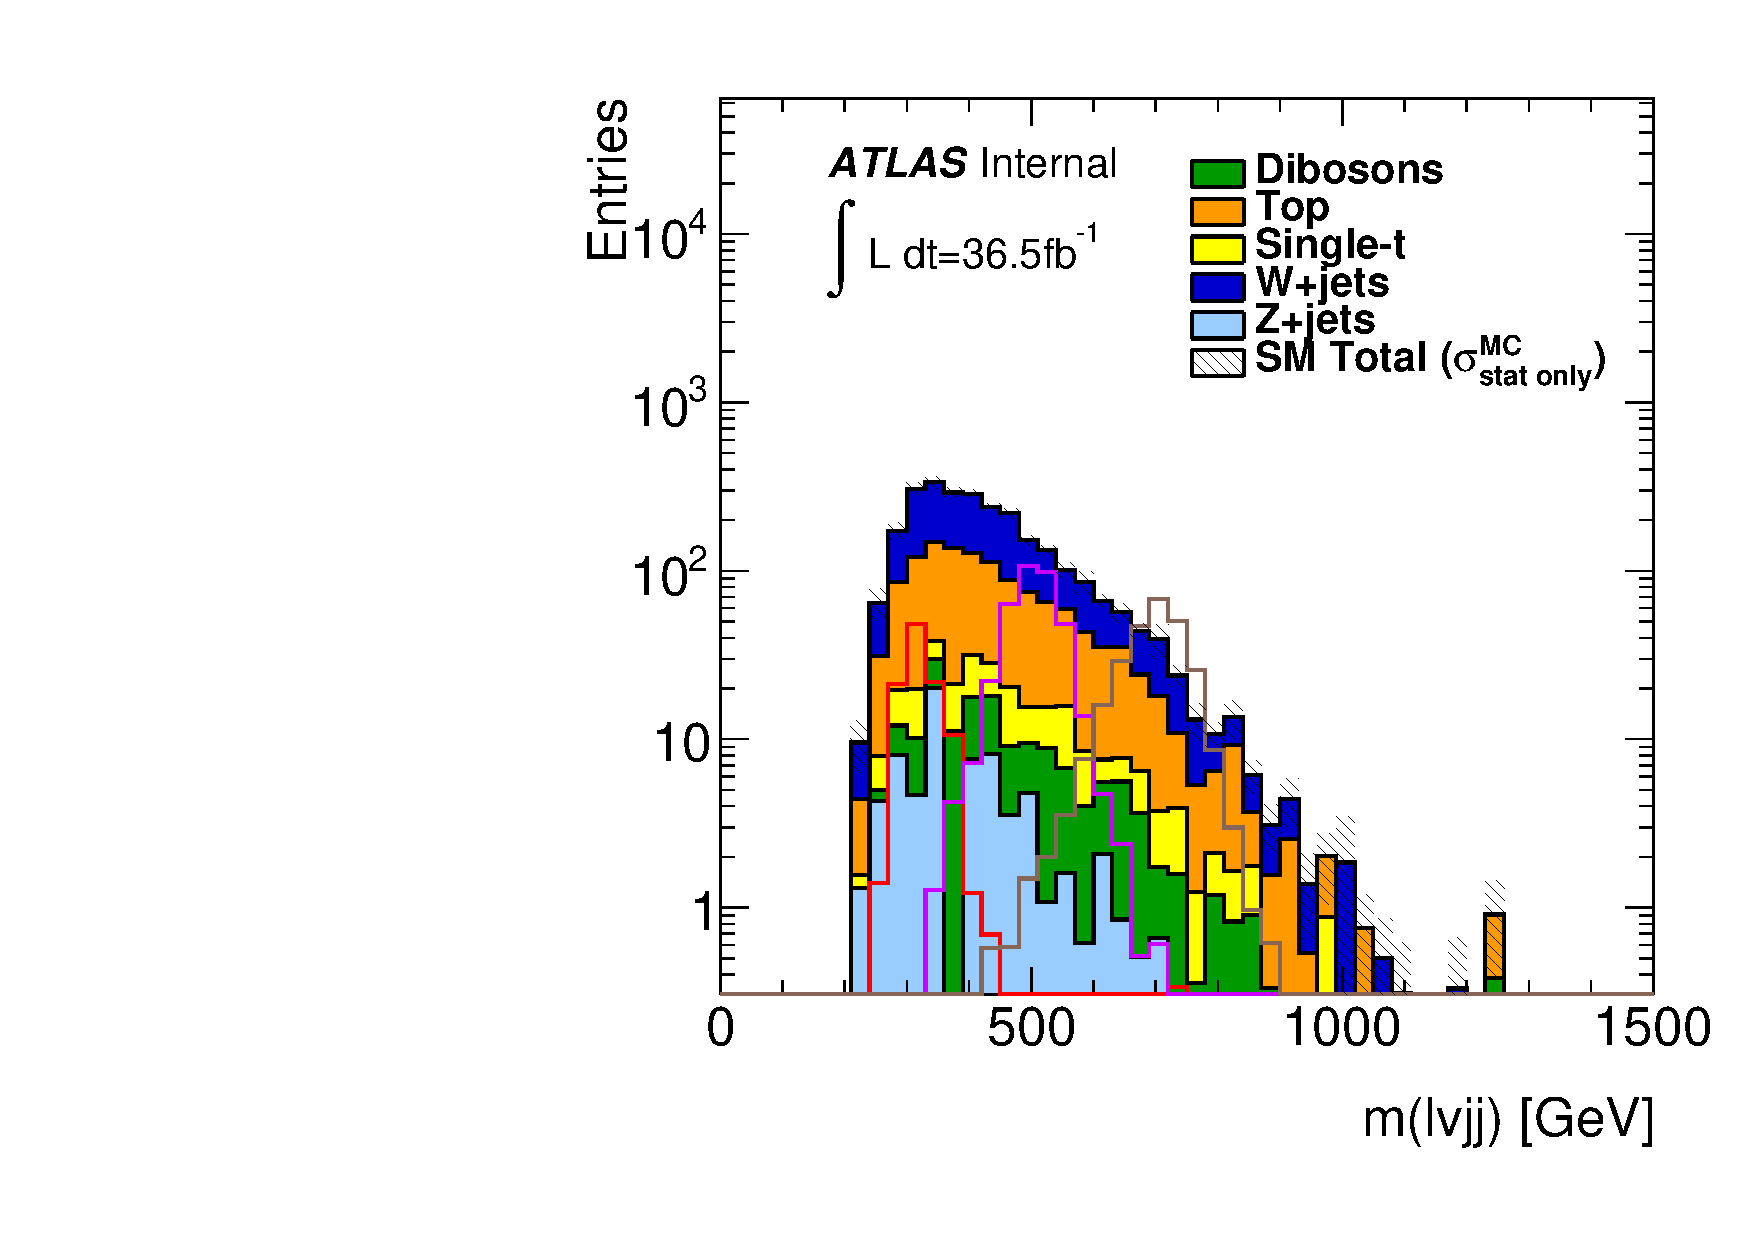
\includegraphics[width=0.5\hsize]{Chapter3/lvjjmass_VBF}}
	\caption{The $m_{WV}$ distribution in the resolved signal region for (a) ggF and (b) VBF channel, with the integrated luminosity of $36.5~fb^{-1}$.The HVT $WZ$ signals with $m=300GeV$ (red), $500GeV$ (violet) and $700GeV$ (blue) are overlaid 
		scaled to $100 ~\times$ cross section.}
	\label{Fig:ResolvedSR}
\end{figure}

\subsection{Multijet Background Estimation}
\label{sec:multijet_background}
As discussed above, the SM backgrounds are estimated from Monte-Carlo simulation and constrained in the dedicated control regions. However, multijet processes is poorly modelled due to the lack of understanding to QCD, so simulation is not feasible for this background contribution. Its contribution is from the following sources:
\begin{itemize}
	\item {\bf Photon Conversion}: When photons or pions interact with the detector material, they decay to soft leptons with similar behaviour to signal ones, which is difficult to recognize. This contribution is mainly into electron, while it could be suppressed by combined muon requirement in muon channel
	\item {\bf Lepton Misidentification}: Soft charged partons could be blocked at ECAL and leave no signature in HCAL, which is identical to electron signatures. In this case, they are reconstructed as electrons instead of jets. This source only contributes to electron channel.
	\item {\bf Heavy Hadron Decay}: The decay products of heavy partons also include leptons. If their decay is close to the primary vertex, the decayed leptons are not distinguishable from the prompt ones. Both electrons and muons have the contribution from this source. 
\end{itemize}
\noindent
As an alternative, the estimation is performed with fake factor method, a data-driven approach. It is only significant in resolved channel while begin negligible in boosted channel.  The details of this method could be found in the ATLAS Run2 VHbb analysis~\cite{ATLAS-CONF-2016-091, ATL-COM-PHYS-2016-429}. 

\subsubsection*{Methodology}

In the method, to be orthogonal to the signal and control region, fake factors are estimated in the region with only one small R jet called single jet control region where the existence of fat jet passing the selection is not allowed ($p_{T}^{J}>200GeV$ \&\& $m^{J}>50GeV$) to keep the orthogonality to boosted region. This region is then further divided into two subregions by lepton isolation, as shown in table \ref{tab:LepIsoCR}. With $p_{T}(\mu\nu)<150 GeV$, an isolated muon trigger is applied with quality, $ivarmedium $, so the isolation requirement for inverse muon is tightened to remove the bias. As region $p_{T}(\mu\nu)>150 GeV$ is using $E_{T}^{miss}$ trigger, so the isolation bias is not presents. Fake factors in the dedicated bins are defined as:
\begin{equation}
 f = \frac{N_{event}(SingleJetSigLepCR)}{N_{event}(SingleJetInvLepCR)}
\end{equation}
with the binning in Table~\ref{tab:FFBinning}. Fake factors have the dependence on lepton eta (this dependence is for the consideration of detector homogeneity) and $p_{T}$. Additional binning on $E_{T}^{miss}$ is applied in electron channel. For both channels, fake factor is estimated in two different regions with $p_{T}(\mu\nu)<150 GeV$ and $p_{T}(\mu\nu)>150 GeV$ to achieve better precision. Fake factor is shown as a function of lepton $p_{T}$ in Figure~\ref{fig:fakefactor} for the region of $p_{T}(l\nu)>150 GeV$. It could be noticed that fake factor for electron channel is just up to $p_{T}=190GeV$. For better accuracy, the fake factor for high $p_{T}$ electron is roughly evaluated in $p_{T}$ bins only which is shown in Figure~\ref{fig:fakefactor_el_highPt}.

\begin{table}[h]
  \caption{Isolation for leptons in the single jet control region} \label{tab:LepIsoCR}
  \begin{center}

    \begin{tabular}{ | c | c | c | }
     \hline
                               &   SingleJetSigLepCR   & SingleJetInvLepCR \\ \hline
    electron                   &        TightLH        & MediumLH (!TightLH) \\ \hline
    muon($p_{T}(l\nu)>150 GeV$) &  $Iso_{trk}<0.06$    & $0.06<Iso_{trk}<0.15$ \\ \hline
    muon($p_{T}(l\nu)<150 GeV$) &  $Iso_{trk}<0.06$    & $0.06<Iso_{trk}<0.07$ \\ \hline
\end{tabular}
\end{center}
\end{table}


\begin{table}[h]
  \caption{Binning for electrons and muons to evaluate fake factor} \label{tab:FFBinning}
\begin{center}

\begin{tabular}{ | c | c | c | c |}
    \hline
    channel  & $p_{T}(GeV)$ & $|\eta|$ & $E_{T}^{miss}(GeV)$ \\ \hline
    electron & 27-115 &  & 0, 60, 75, $\infty$ \\
             & 115-135&0, 1.37, 1.52, 2.47 & 0, 38, 52, $\infty$ \\
             & 135-155& & 0, 26, 43, $\infty$ \\
             & 155-190& & 0, 25, 45, $\infty$ \\ \hline
    muon     & 27, 42, 59, 76, 99, $\infty$ & 0, 1.05, 1.5, 2.5 & N/A \\ \hline

\end{tabular}
\end{center}
\end{table}

\begin{figure}[ht]
       \centering
       \subfloat[]{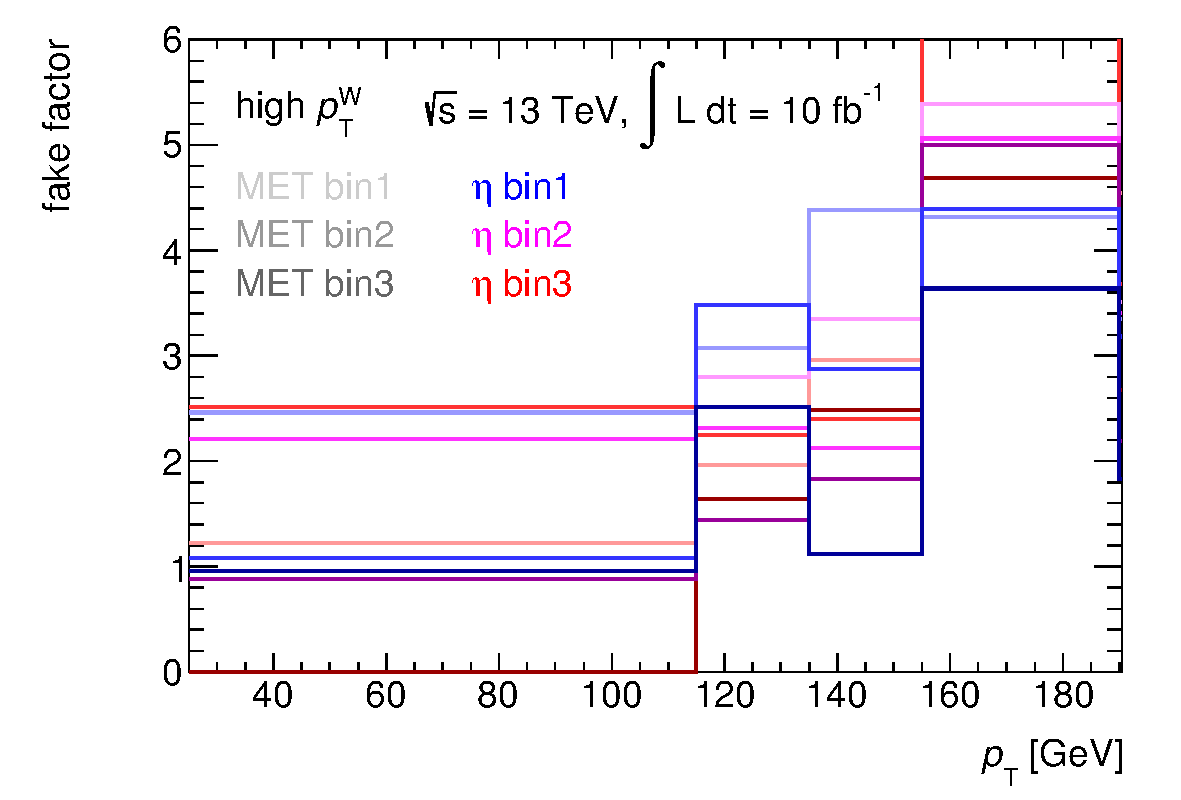
\includegraphics[width=0.4\textwidth]{Chapter3/fakefactor_el_medium_highpTW}}
       \subfloat[]{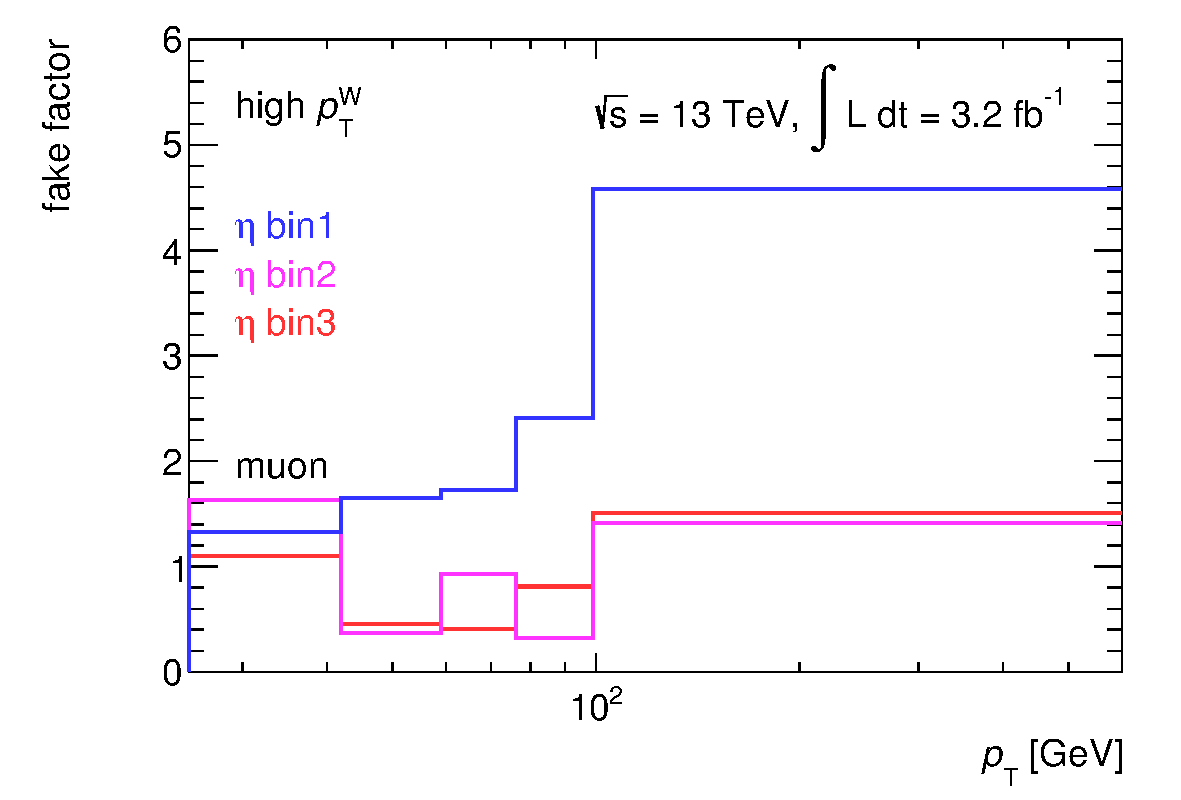
\includegraphics[width=0.4\textwidth]{Chapter3/fakerate_mu_ewk}} \\
       \caption{Fake factors for the corresponding binnings (shown in text) in electron (a) and muon (b) channels}
       \label{fig:fakefactor}
\end{figure}

\begin{figure}[ht]
       \centering
       \subfloat[]{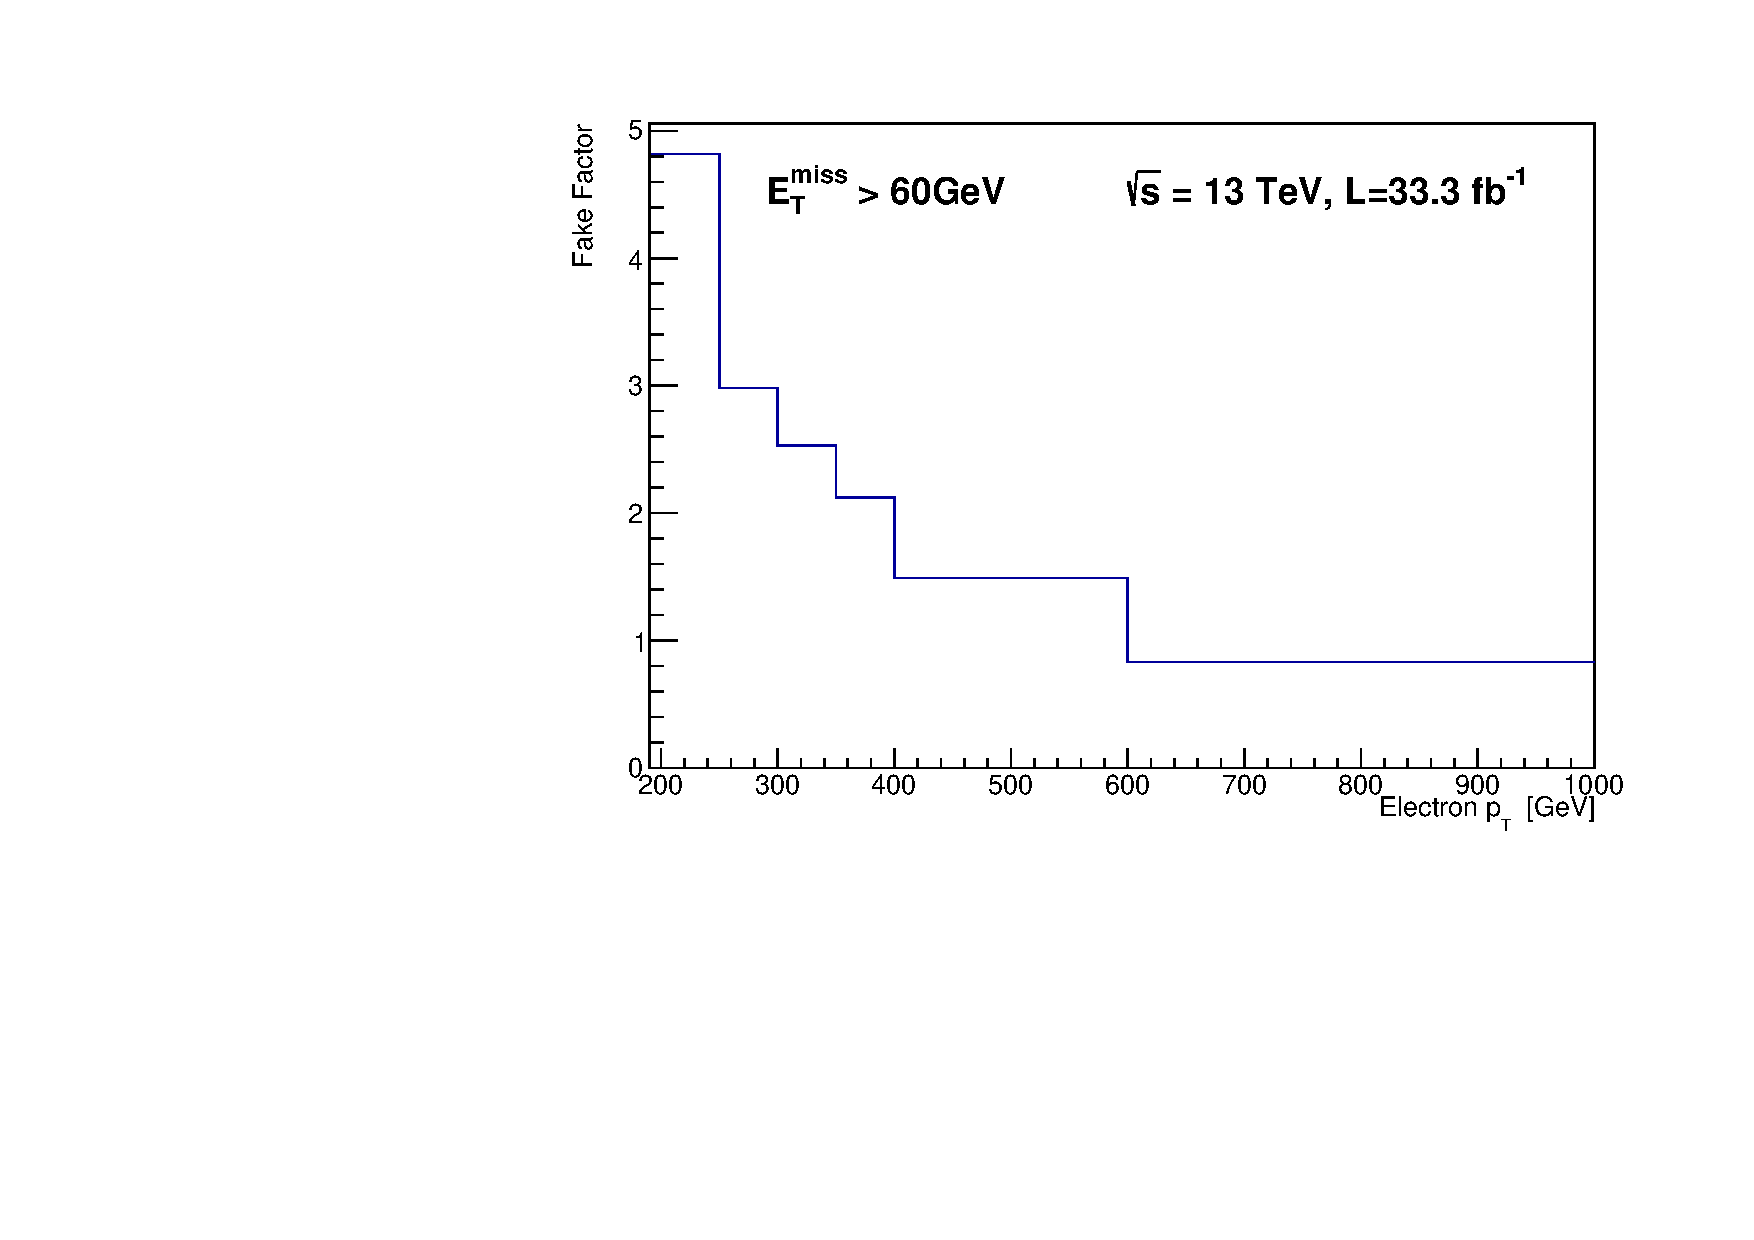
\includegraphics[width=0.4\textwidth]{Chapter3/fakerate_el_highPt.pdf}}
       \caption{Fake factors for high $p_T$ electrons}
       \label{fig:fakefactor_el_highPt}
\end{figure}


\subsubsection*{Electroweak Subtraction}

Electroweak interactions ($t\bar{t}$, W/Z+jets, diboson and single top) could also contribute to multijet events in addition to the multijet background, so they might be double counted from fake factor estimation and Monte Carlo simulation. To avoid this issue, those events are removed by employing fake factor estimation on Monte Carlo samples, which could be expressed as the following equation:
\begin{equation}
 N^{MJ}_{events} = N^{data}_{events}-N^{MC}_{event}
\end{equation}
Unfortunately, it is observed that the multijet behavior is not well-modeled in simulation with $E_{T}^{miss}>150 GeV$ for SM backgrounds. This is verified in dijet inversed lepton control region with lepton isolation inversed and at least two jets with $P_{T}>20GeV$. Figure~\ref{fig:dijetFakeCR_el} and Figure~\ref{fig:dijetFakeCR_mu} show the discrepancy between data and electroweak interactions which are contributed from multijet events. It is anticipated that multijet contribution shall be almost 0 in high $E^{miss}_{T}$ region in the dijet control region, but the discrepancy is still observed. In this case, the electroweak subtraction is applied with a scale factor derive from the ratio of events from data and simulation in the bin $150 GeV<E^{miss}_{T}<250GeV$ defined as: 
\begin{equation}
f = \frac{N_{event}(data)}{N_{event}(MC)}
\end{equation}
It is applied as an additional correction on fake factor for events with $E_{T}^{miss}>150 GeV$ from simulation. The electroweak subtraction factors for electron and muon channels are shown in Table~\ref{tab:ewsubtraction}.

\begin{figure}[ht]
       \centering
       \subfloat[]{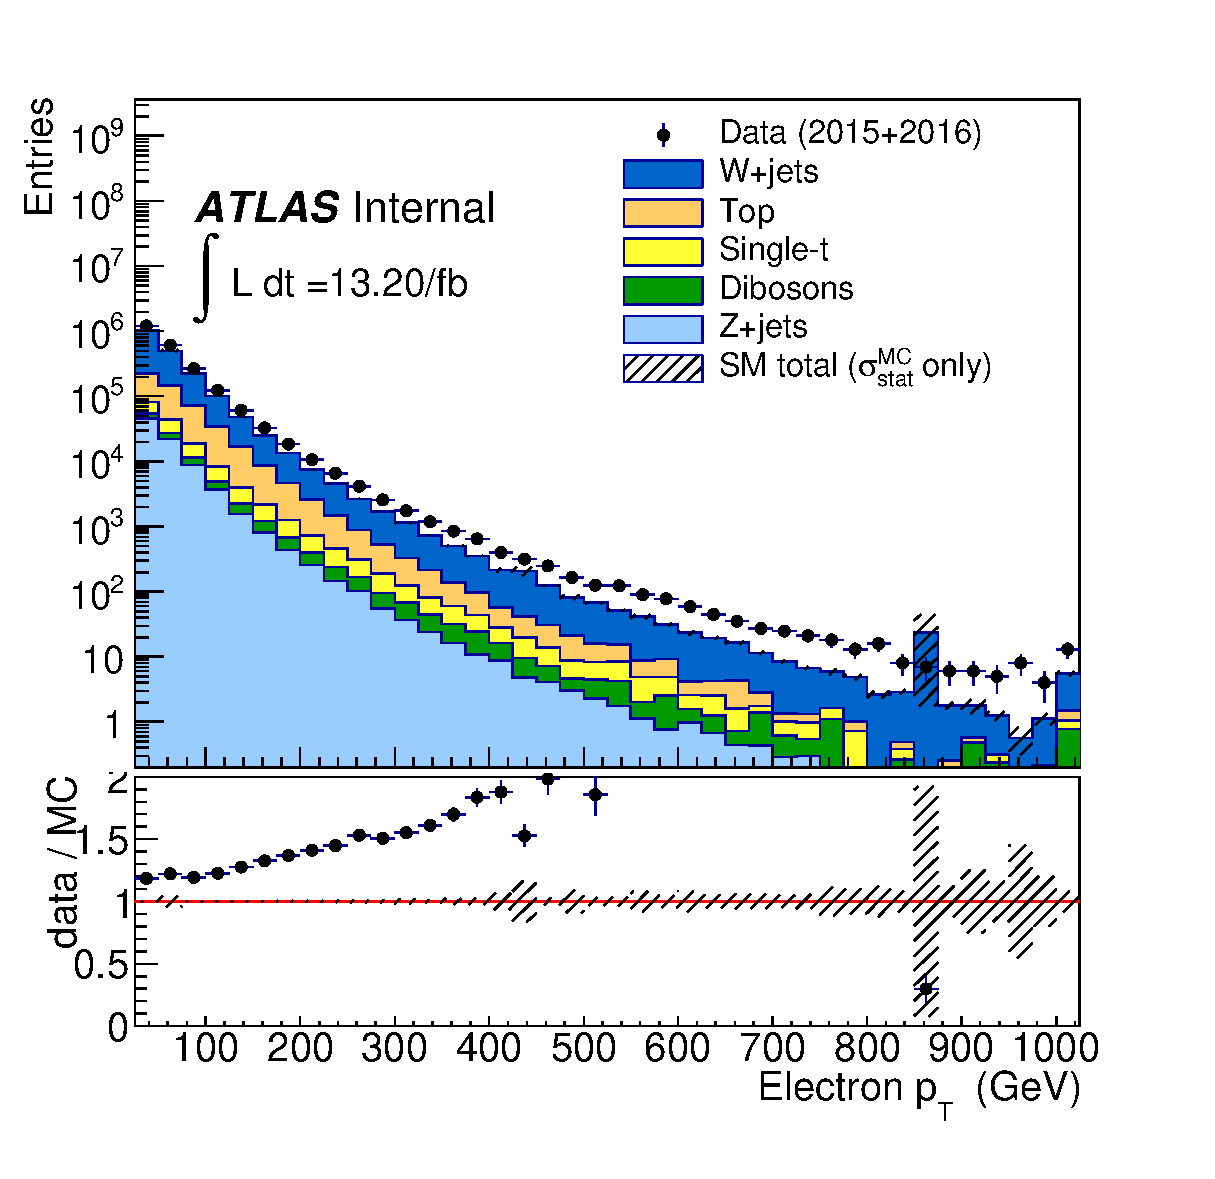
\includegraphics[width=0.45\textwidth]{Chapter3/MJ_CR/electronPt.eps}}
       \subfloat[]{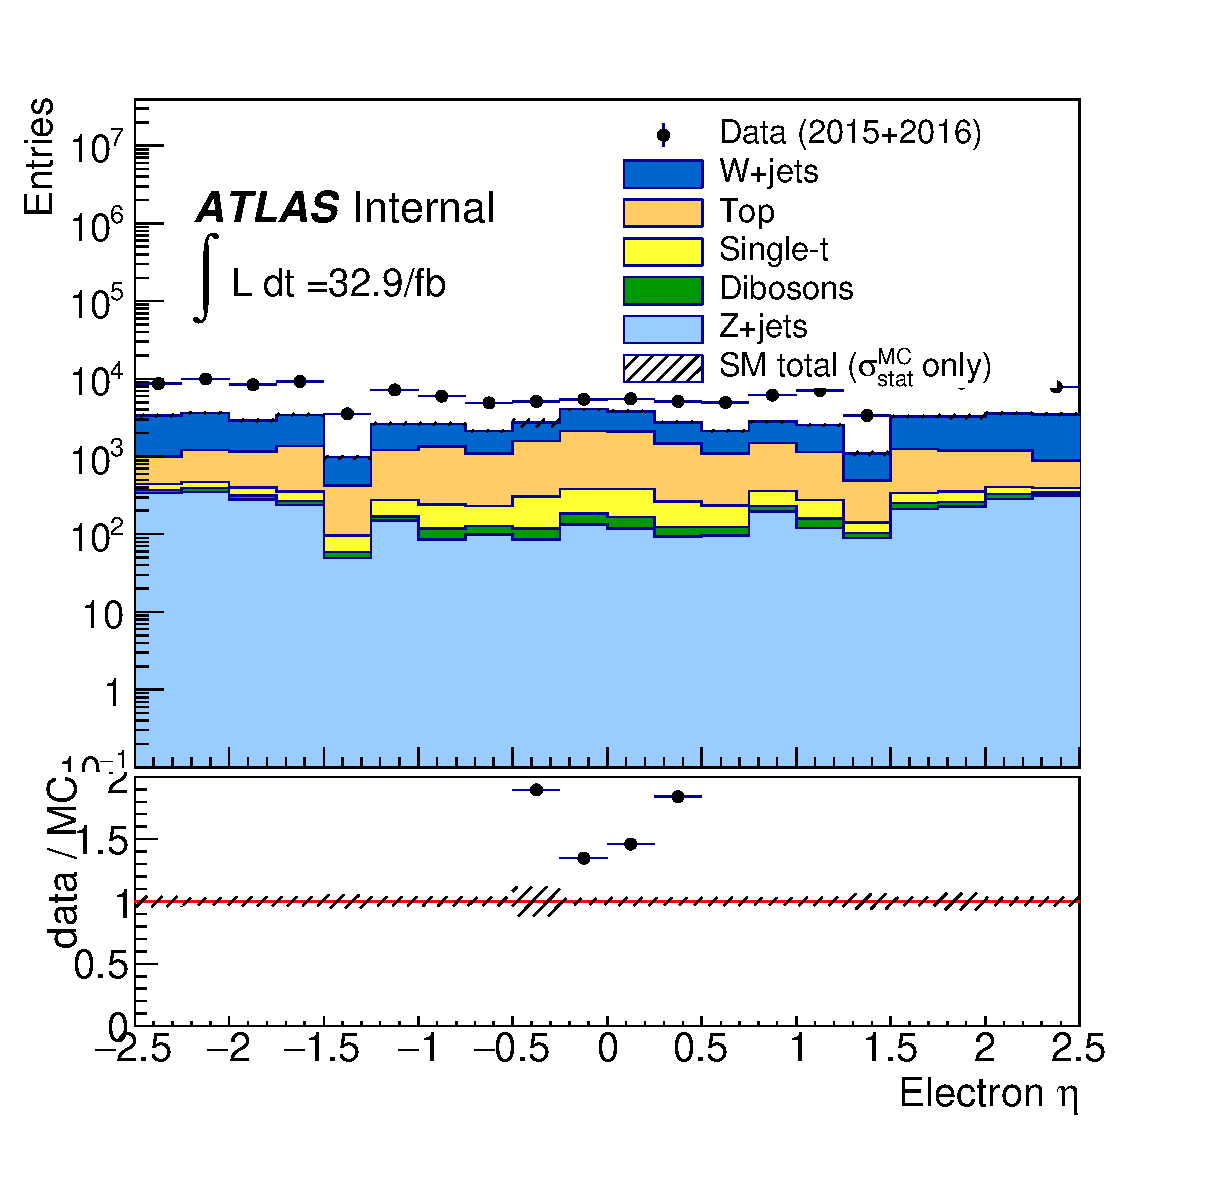
\includegraphics[width=0.45\textwidth]{Chapter3/MJ_CR/electronEta.eps}}\\ 
       \subfloat[]{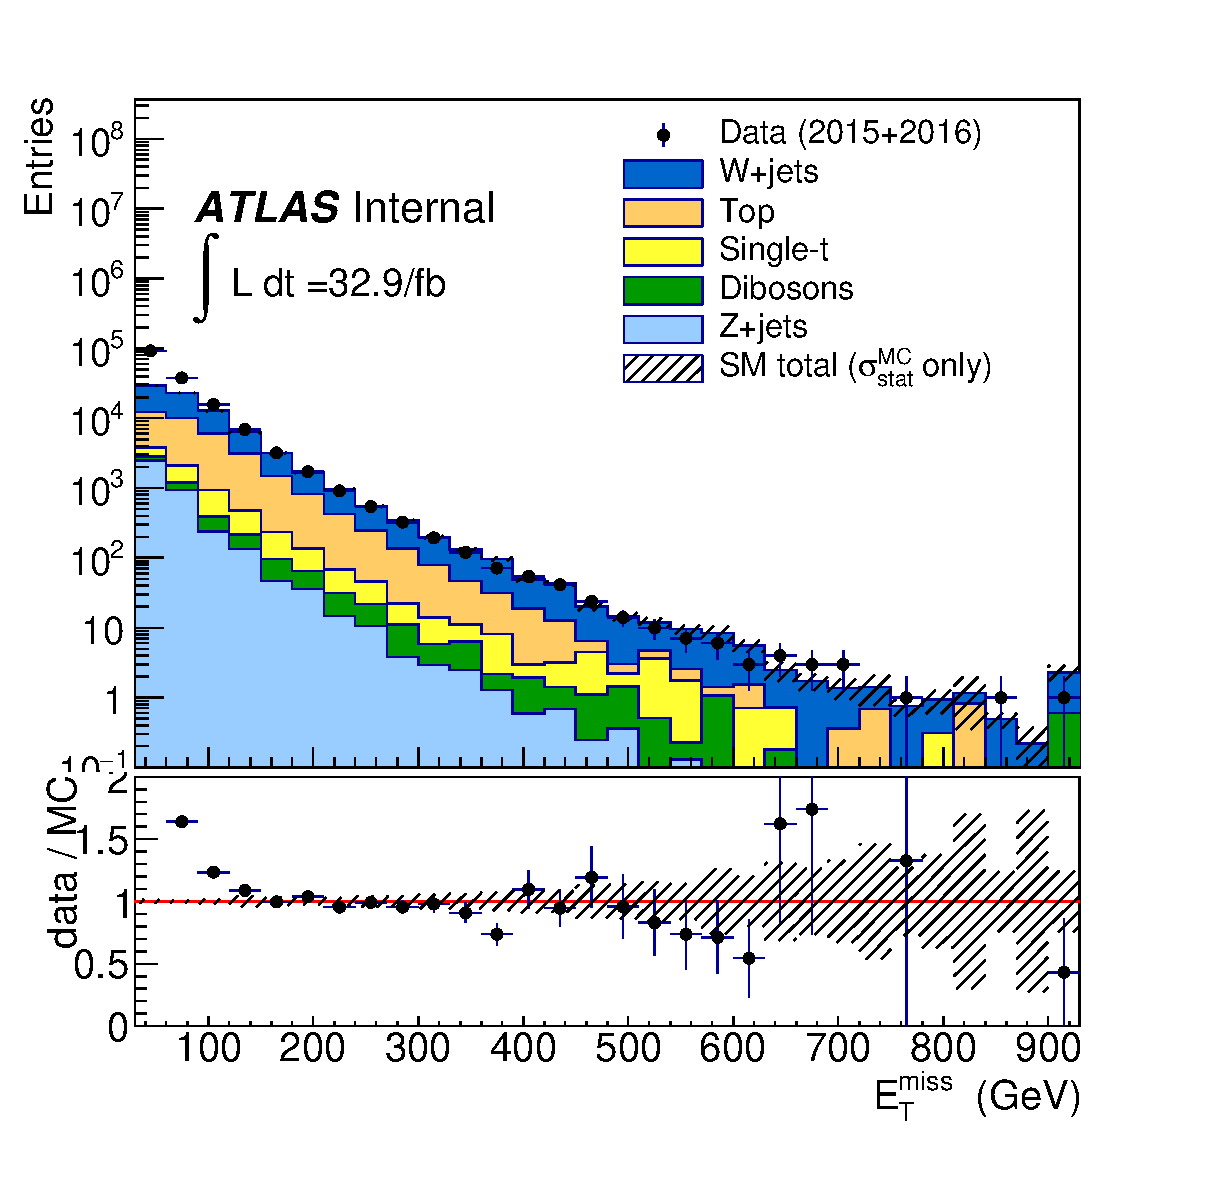
\includegraphics[width=0.45\textwidth]{Chapter3/MJ_CR/met_el.eps}}
       \subfloat[]{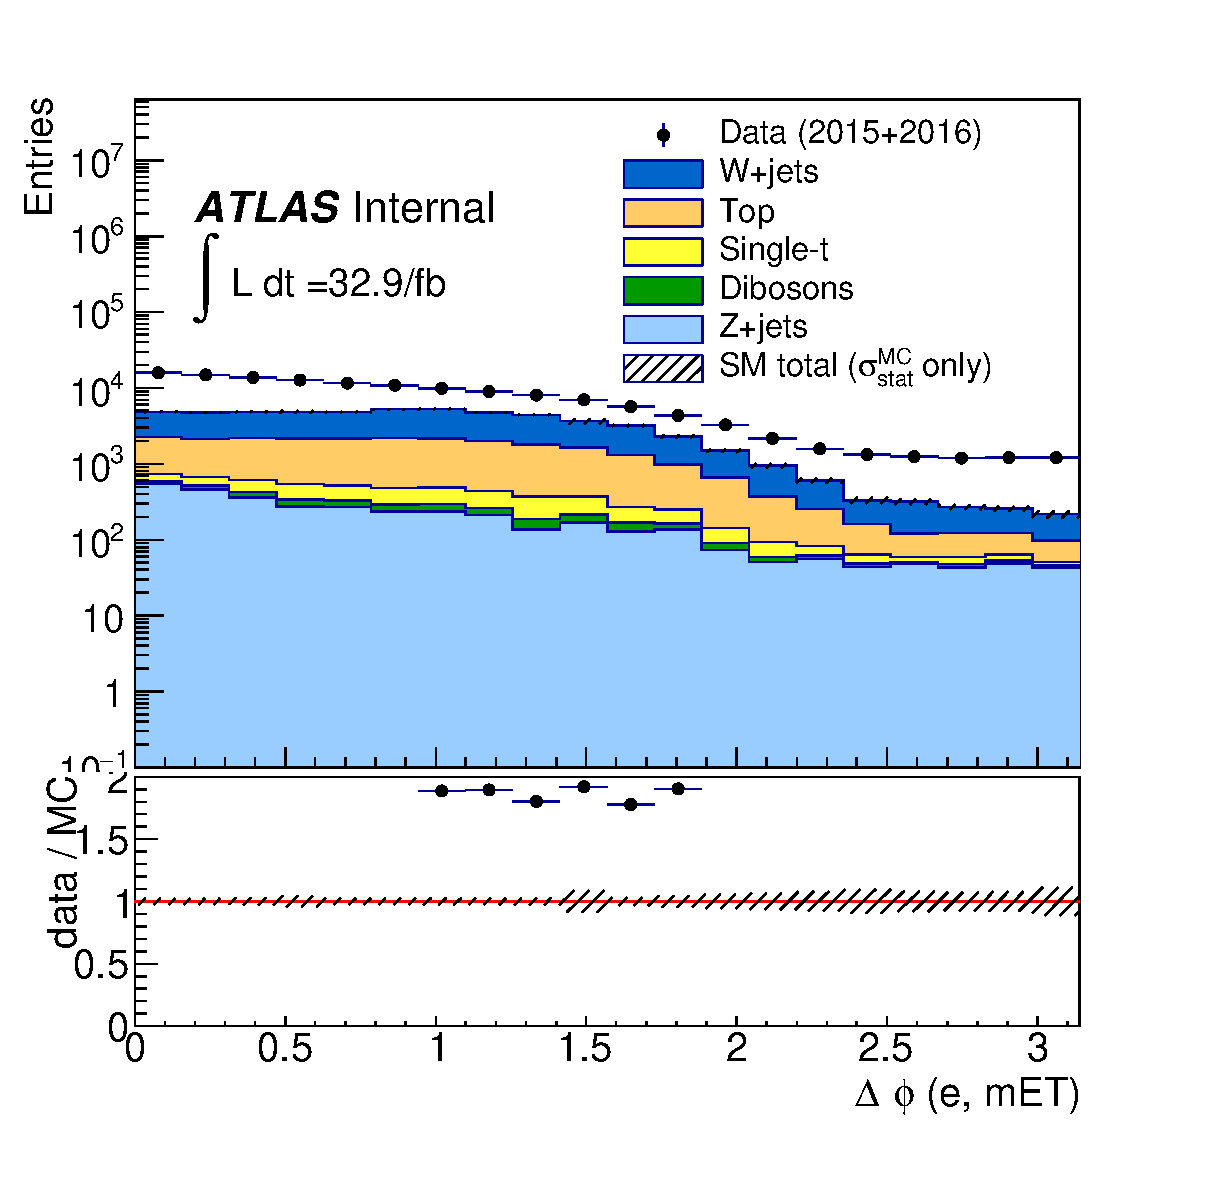
\includegraphics[width=0.45\textwidth]{Chapter3/MJ_CR/dphilepmet_el.eps}}\\
       \caption{The distribution of lepton $p_{T}$,$\eta$, $E_{T}^{miss}$ and $\Delta\phi$(e,$E_{T}^{miss}$) in dijet fake control region with inversed lepton for electron channel. The inconsistency is thought to be comprised of multijet events without applying electroweak subtraction.} 
       \label{fig:dijetFakeCR_el}
\end{figure}

\begin{figure}[ht]
       \centering
       \subfloat[]{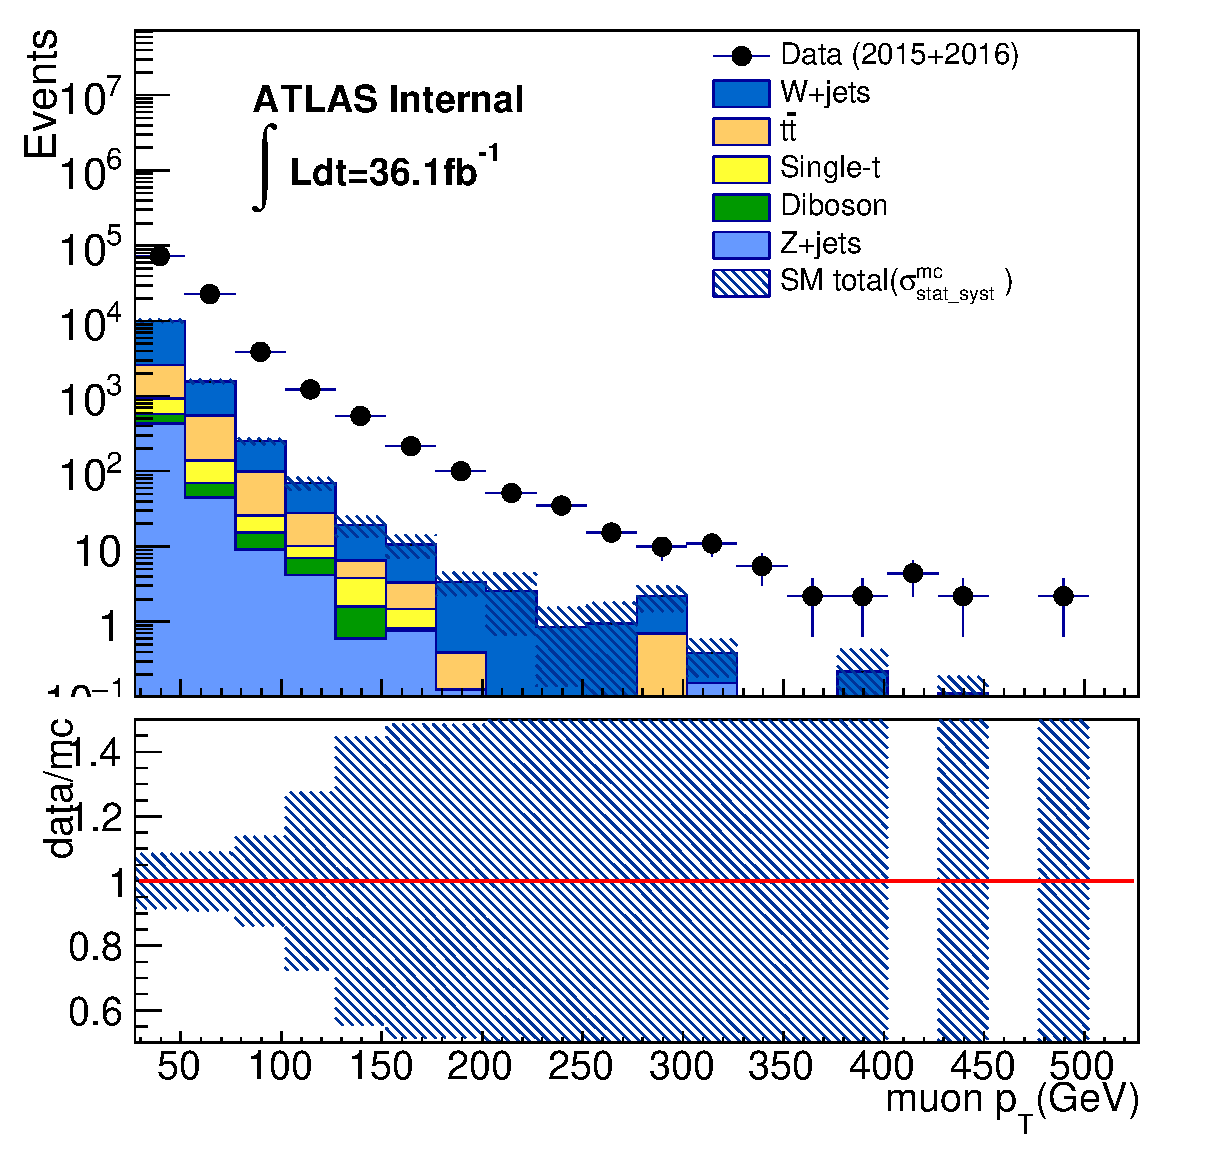
\includegraphics[width=0.45\textwidth]{Chapter3/MJ_CR/muonPt.eps}}
       \subfloat[]{\includegraphics[width=0.45\textwidth]{Chapter3/MJ_CR/muonEta.eps}} \\
       \subfloat[]{\includegraphics[width=0.45\textwidth]{Chapter3/MJ_CR/met_mu.eps}}
       \subfloat[]{\includegraphics[width=0.45\textwidth]{Chapter3/MJ_CR/dphilepmet_mu.eps}}\\
       \caption{The distribution of lepton $p_{T}$,$\eta$, $E_{T}^{miss}$ and $\Delta\phi$($\mu$,$E_{T}^{miss}$) in dijet fake control region with inversed lepton for muon channel. The inconsistency is thought to be comprised of multijet events without applying electroweak subtraction.}
       \label{fig:dijetFakeCR_mu}
\end{figure}

\begin{table}[h]
  \caption{Electroweak subtraction factor for electron and muon channels} \label{tab:ewsubtraction}
  \begin{center}

    \begin{tabular}{ | c | c | c | }
     \hline
     channels                       &   electron   & muon \\ \hline
     EW subtraction factor          &   1.36       & 1.49 \\ \hline
\end{tabular}
\end{center}
\end{table}

\subsubsection*{Validation}
The method is validated in the dedicated validation region. The definition is similar to the signal region with looser cut to enrich the multijet events. It requires at lease two resolved jets ($p_{T}^{leading}>60GeV$, $p_{T}^{subleading}>45GeV$), $30GeV<E^{miss}_{T}<50GeV$, exactly one isolated lepton and the resolved triggers passed for electron and muon channels respectively. This definition is slightly overlapped with signal and control regions, but the upper cut on $E^{miss}_{T}$ suppress the signal contribution.  As the fake factors were derived from two bins of $p_{T}(l\nu)$, the validation is performed on $p_{T}(l\nu)<150 GeV$ and $p_{T}(l\nu)>150 GeV$. The results are presented in Figures~\ref{fig:FakeVR1_el} -~\ref{fig:FakeVR2_mu} with multijet background estimated using fake factor method. In general, data agrees well with backgrounds with tolerable inconsistency within statistic uncertainties. The disagreement in the region of $p_{T}(l\nu)>150 GeV$ is supposed to be due to the low statistics for fake factor estimation in single jet control region, but it should not have great impact in final interpretation, as multijet events would just account for around 10\% of the whole background. The related systematic uncertainty would be discussed in Chapter~\ref{Ch:resonance_stat}.
\clearpage
\begin{figure}[ht]
	\centering
	\subfloat[]{\includegraphics[width=0.43\textwidth]{Chapter3/MJ_VR/lep1pt_Loose_el_highWpt}}
	\subfloat[]{\includegraphics[width=0.43\textwidth]{Chapter3/MJ_VR/lep1eta_Loose_el_highWpt}}\\
	\subfloat[]{\includegraphics[width=0.43\textwidth]{Chapter3/MJ_VR/met_Loose_el_highWpt}}
	\subfloat[]{\includegraphics[width=0.43\textwidth]{Chapter3/MJ_VR/dphilepmet_Loose_el_highWpt}}\\
	\subfloat[]{\includegraphics[width=0.43\textwidth]{Chapter3/MJ_VR/lvjjmass_Loose_el_highWpt}}
	\caption{The distribution of lepton $p_{T}$,$\eta$, $E_{T}^{miss}$, $\Delta\phi$(e,$E_{T}^{miss}$), $m_{WV}$in validation region with $p_{T}(l\nu)>150 GeV$ in electron channel with multijet background}
	\label{fig:FakeVR1_el}
	
\end{figure}
\clearpage
\begin{figure}[ht]
	\centering
	\subfloat[]{\includegraphics[width=0.43\textwidth]{Chapter3/MJ_VR/lep1pt_Loose_el_lowWpt}}
	\subfloat[]{\includegraphics[width=0.43\textwidth]{Chapter3/MJ_VR/lep1eta_Loose_el_lowWpt}}\\
	\subfloat[]{\includegraphics[width=0.43\textwidth]{Chapter3/MJ_VR/met_Loose_el_lowWpt}}
	\subfloat[]{\includegraphics[width=0.43\textwidth]{Chapter3/MJ_VR/dphilepmet_Loose_el_lowWpt}}\\
	\subfloat[]{\includegraphics[width=0.43\textwidth]{Chapter3/MJ_VR/lvjjmass_Loose_el_lowWpt}}
	\caption{The distribution of lepton $p_{T}$,$\eta$, $E_{T}^{miss}$, $\Delta\phi$(e,$E_{T}^{miss}$), $m_{WV}$ and BDT in validation region with $p_{T}(l\nu)<150 GeV$ in electron channel with multijet background}
	\label{fig:FakeVR2_el}
\end{figure}
\clearpage
\begin{figure}[ht]
	\centering
	\subfloat[]{\includegraphics[width=0.43\textwidth]{Chapter3/MJ_VR/lep1pt_Loose_mu_highWpt.eps}}
	\subfloat[]{\includegraphics[width=0.43\textwidth]{Chapter3/MJ_VR/lep1eta_Loose_mu_highWpt.eps}}\\
	\subfloat[]{\includegraphics[width=0.43\textwidth]{Chapter3/MJ_VR/met_Loose_mu_highWpt.eps}}
	\subfloat[]{\includegraphics[width=0.43\textwidth]{Chapter3/MJ_VR/dphilepmet_Loose_mu_highWpt.eps}}\\
	\subfloat[]{\includegraphics[width=0.43\textwidth]{Chapter3/MJ_VR/lvjjmass_Loose_mu_highWpt.eps}}
	\caption{The distribution of lepton $p_{T}$,$\eta$, $E_{T}^{miss}$, $\Delta\phi$($\mu$,$E_{T}^{miss}$), $m_{WV}$ and BDT in validation region with $p_{T}(l\nu)>150 GeV$ in muon channel with multijet background}
	\label{fig:FakeVR1_mu}
\end{figure}
\clearpage
\begin{figure}[ht]
	\centering
	\subfloat[]{\includegraphics[width=0.43\textwidth]{Chapter3/MJ_VR/lep1pt_Loose_mu_lowWpt.eps}}
	\subfloat[]{\includegraphics[width=0.43\textwidth]{Chapter3/MJ_VR/lep1eta_Loose_mu_lowWpt.eps}}\\
	\subfloat[]{\includegraphics[width=0.43\textwidth]{Chapter3/MJ_VR/met_Loose_mu_lowWpt.eps}}
	\subfloat[]{\includegraphics[width=0.43\textwidth]{Chapter3/MJ_VR/dphilepmet_Loose_mu_lowWpt.eps}}\\
	\subfloat[]{\includegraphics[width=0.43\textwidth]{Chapter3/MJ_VR/lvjjmass_Loose_mu_lowWpt.eps}}
	\caption{The distribution of lepton $p_{T}$,$\eta$, $E_{T}^{miss}$, $\Delta\phi$($\mu$,$E_{T}^{miss}$), $m_{WV}$ and BDT in validation region with $p_{T}(l\nu)<150 GeV$ in muon channel with multijet background}
	\label{fig:FakeVR2_mu}
\end{figure}
\clearpage
\section{Data Background Comparison}
\label{Sec:data_bkg_compar}
To verify the modelling of background estimation, the comparison in top and W+jet control regions are performed for both VBF and ggF categories. The consistency is not perfect as expectation, and the fitting in the control regions is on the purpose to recover it, which will be discussed in next chapter. The other issue in the background simulation is that a slope in the ratio of data over background is observed in $m^{VBF}_{jj}$ in resolved VBF category for V+jet samples from Sherpa generator. In this analysis, it is also taken as one contribution to the mismodelling of simulation. 
\\
\\Fig. \ref{Fig:ggFWR} and Fig. \ref{Fig:ggFTR} are the comparison plots for $m_{WV}$ in ggF category, while Fig. \ref{Fig:mWVVBFWR} to Fig. \ref{Fig:mWVVBFTR} are for VBF category. The comparison of  $m^{VBF}(j,j)$ could be found in Fig. \ref{Fig:mJJVBFWR} and Fig. \ref{Fig:mJJVBFTR} to examine the VBF modelling. 
\newpage

\begin{figure}[ht]
	\centering
	\subfloat[]{\includegraphics[width=0.43\textwidth]{Chapter3/HighPurityCR_36fb/VVM_3_el}}
	\subfloat[]{\includegraphics[width=0.43\textwidth]{Chapter3/HighPurityCR_36fb/VVM_3_mu}}\\
	\subfloat[]{\includegraphics[width=0.43\textwidth]{Chapter3/LowPurityCR_36fb/VVM_12_el}}
	\subfloat[]{\includegraphics[width=0.43\textwidth]{Chapter3/LowPurityCR_36fb/VVM_12_mu}}\\
    \subfloat[]{\includegraphics[width=0.43\textwidth]{Chapter3/ResolvedCR/ggF36fb/VVM_5_el}}
	\subfloat[]{\includegraphics[width=0.43\textwidth]{Chapter3/ResolvedCR/ggF36fb/VVM_5_mu.eps}}
	\caption{The distribution of $m_{WV}$ in ggF high purity (top), low purity (middle), and resolved (bottom) W+jet control region for electron (left) and muon (right) channels respectively}
	\label{Fig:ggFWR}
\end{figure}



\begin{figure}[ht]
	\centering
	\subfloat[]{\includegraphics[width=0.43\textwidth]{Chapter3/HighPurityCR_36fb/VVM_2_el}}
	\subfloat[]{\includegraphics[width=0.43\textwidth]{Chapter3/HighPurityCR_36fb/VVM_2_mu}}\\
	\subfloat[]{\includegraphics[width=0.43\textwidth]{Chapter3/LowPurityCR_36fb/VVM_13_el}}
    \subfloat[]{\includegraphics[width=0.43\textwidth]{Chapter3/LowPurityCR_36fb/VVM_13_mu}}\\
	\subfloat[]{\includegraphics[width=0.43\textwidth]{Chapter3/ResolvedCR/ggF36fb/VVM_6_el}}
    \subfloat[]{\includegraphics[width=0.43\textwidth]{Chapter3/ResolvedCR/ggF36fb/VVM_6_mu.eps}}
	\caption{The distribution of $m_{WV}$ in ggF high purity (top), low purity (middle), and resolved (bottom) top control region for electron (left) and muon (right) channels respectively}
	 \label{Fig:ggFTR}
\end{figure}


\begin{figure}[ht]
	\centering
	\subfloat[]{\includegraphics[width=0.43\textwidth]{Chapter3/VBF36fbHP/VVM_3_el}}
	\subfloat[]{\includegraphics[width=0.43\textwidth]{Chapter3/VBF36fbHP/VVM_3_mu}}\\
	\subfloat[]{\includegraphics[width=0.43\textwidth]{Chapter3/VBF36fbLP/VVM_12_el}}
    \subfloat[]{\includegraphics[width=0.43\textwidth]{Chapter3/VBF36fbLP/VVM_12_mu}}\\	
	\subfloat[]{\includegraphics[width=0.43\textwidth]{Chapter3/ResolvedCR/VBF36fb/VVM_5_el}}
    \subfloat[]{\includegraphics[width=0.43\textwidth]{Chapter3/ResolvedCR/VBF36fb/VVM_5_mu.eps}}    
	\caption{The distribution of $m_{WV}$ in VBF high purity (top), low purity (middle), and resolved (bottom) W+jet control region for electron (left) and muon (right) channels respectively}
	\label{Fig:mWVVBFWR}
\end{figure}
\clearpage
\begin{figure}[ht]
	\centering

	\subfloat[]{\includegraphics[width=0.43\textwidth]{Chapter3/VBF36fbHP/VBFmass_3_el}}
	\subfloat[]{\includegraphics[width=0.43\textwidth]{Chapter3/VBF36fbHP/VBFmass_3_mu}}\\
	\subfloat[]{\includegraphics[width=0.43\textwidth]{Chapter3/VBF36fbLP/VBFmass_12_el}}
    \subfloat[]{\includegraphics[width=0.43\textwidth]{Chapter3/VBF36fbLP/VBFmass_12_mu}}\\	
 	\subfloat[]{\includegraphics[width=0.43\textwidth]{Chapter3/ResolvedCR/VBF36fb/VBFmass_5_el}}
    \subfloat[]{\includegraphics[width=0.43\textwidth]{Chapter3/ResolvedCR/VBF36fb/VBFmass_5_mu}}\\   
	\caption{The distribution of $m_{jj}^{VBF}$ in VBF high purity (top), low purity (middle), and resolved (bottom) W+jet control region for electron (left) and muon (right) channels respectively}
	\label{Fig:mJJVBFWR}
\end{figure}


\begin{figure}[ht]
	\centering
	\subfloat[]{\includegraphics[width=0.43\textwidth]{Chapter3/VBF36fbHP/VVM_2_el}}
	\subfloat[]{\includegraphics[width=0.43\textwidth]{Chapter3/VBF36fbHP/VVM_2_mu}}\\
	\subfloat[]{\includegraphics[width=0.43\textwidth]{Chapter3/VBF36fbLP/VVM_13_el}}
    \subfloat[]{\includegraphics[width=0.43\textwidth]{Chapter3/VBF36fbLP/VVM_13_mu}}\\
	\subfloat[]{\includegraphics[width=0.43\textwidth]{Chapter3/ResolvedCR/VBF36fb/VVM_6_el}}
    \subfloat[]{\includegraphics[width=0.43\textwidth]{Chapter3/ResolvedCR/VBF36fb/VVM_6_mu.eps}}	
	\caption{The distribution of $m_{WV}$ in VBF high purity (top), low purity (middle), and resolved (bottom) top control region for electron (left) and muon (right) channels respectively}
	\label{Fig:mWVVBFTR}
\end{figure}
\clearpage
\begin{figure}[ht]
	\centering
	\subfloat[]{\includegraphics[width=0.43\textwidth]{Chapter3/VBF36fbHP/VBFmass_2_el}}
	\subfloat[]{\includegraphics[width=0.43\textwidth]{Chapter3/VBF36fbHP/VBFmass_2_mu}}\\
	\subfloat[]{\includegraphics[width=0.43\textwidth]{Chapter3/VBF36fbLP/VBFmass_13_el}}
    \subfloat[]{\includegraphics[width=0.43\textwidth]{Chapter3/VBF36fbLP/VBFmass_13_mu}}\\	
    \subfloat[]{\includegraphics[width=0.43\textwidth]{Chapter3/ResolvedCR/VBF36fb/VBFmass_6_el}}
    \subfloat[]{\includegraphics[width=0.43\textwidth]{Chapter3/ResolvedCR/VBF36fb/VBFmass_6_mu}}\\
	\caption{The distribution of $m_{jj}^{VBF}$ in VBF high purity (top), low purity (middle), and resolved (bottom) top control region for electron (left) and muon (right) channels respectivelyy}
	\label{Fig:mJJVBFTR}
\end{figure}


 	\let\cleardoublepage\clearpage
 	\chapter{Interpretation for Resonance Analysis}
\chapterquote{The best things happen by chance.}{Dory, Finding Dory}
\label{Ch:resonance_stat}
After obtaining the $m_{WV}$ distributions from both control and signal regions, a statistical interpretation is used to determine whether any signal signature is captured in this analysis. The statistical analysis uses the following steps:

\begin{itemize}
	\item{Variation on Histograms}: Systematic uncertainties are applied in the analysis to vary the variables like the jet energy or event weight on the simulation samples. This then leads to the variations on distribution of $m_WV$, and each systematic uncertainty gives one varied $m_{WV}$ histogram. Those histograms are then taken into the statistic interpretation with the one without any variation (this is called ``nominal'' histogram) for following steps. 

	\item{Simultaneous Fitting}: a binned maximum-likelihood fitting is performed in control and signal region histograms simultaneously to rescale the backgrounds and signal for a proper agreement to the data. The scaling is performed bin-by-bin in histograms of $m_{WV}$ distribution, which means the shape of $m_{WV}$ distribution would change under this step. Further detail will be discussed later.
	
	\item{Signal Verification}: the signal interpretation is through the CLs method by quantifying the agreement between data and background in signal regions after simultaneous fitting. The result will be presented as the exclusion on the mass regions at $95\%$ confidence level or the discovery with a corresponding ``p-value''.
\end{itemize}
The details of each step will be discussed in the following sections with the results from this analysis, and the details of the methodology formalism can be referred to \cite{StatisticsData}.
\section{Systematic Uncertainties}
No measurement and theoretical estimation could be $100\%$ accurate, and the uncertainties would propagate to the $m_{WV}$ histograms. In this case, a bump in data might be due to the uncertainty fluctuation but mistaken as a signal. To prevent such a mistake, both systematic and statistic uncertainties are brought into the consideration for the ground fitting and signal interpretation. The following are the systematic uncertainties considered in this analysis and how they are taken into the $m_{WV}$ histograms, and the methods to estimate the uncertainties of each source could be found in \cite{PERF-2016-01,ATL-PHYS-PUB-2015-037,ATLAS:2019pzw,PERF-2016-04,ATLAS-CONF-2014-018,Herde:2059849}.
\begin{itemize}
	\item{\bf Luminosity Measurement}: the given luminosity of the dataset collected in 2015 and 2016 is accompanied by the uncertainty of $2.1\%$. It is applied in the histograms from simulations by scaling up and down the total yield of each bin by $2.1\%$.

	\item{\bf Selection and Reconstruction Efficiency}: the object reconstruction and selection efficiency of physical objects are not consistent between data and simulation like the trigger efficiency shown in Subsec.~\ref{Subsec:Trigger_resonance}. This type of uncertainties are induced by the uncertainties in variables used in tag and probe method. To estimate the impact, the tag and probe criteria are tightened and loosened for scale factor re-estimation, and they replace the nominal scale factors to obtain the new histograms. This type of uncertainties come from the efficiencies of trigger, lepton isolation, lepton identification, jet b-tagging, fat jet boson-tagging, and all physical object reconstruction, and each of them gives one uncertainty contribution with a pair of histograms. (loosened and tightened criteria give two histograms for each source.)

	\item{\bf Energy Scale and Resolution}: the energy measurement is based on the pulse shapes from the calorimeter cells, but it is not precise enough due to different responses of layers or varied granularities of the calorimeter. The uncertainty estimation of this source for electrons and muons are via the $Z$ boson mass reconstruction in dedicated analysis as a function of $p_{T}$. In the case of jets, they are estimated via the comparison of the MC truth and reconstructed $E_{T}$ from dijet simulation samples with the variation on multiple sources, which contributes 81 uncertainties. However, a simplified scheme is applied to combine related uncertainties into 21 categories, for which details could be found in \cite{Herde:2059849}. The measurement uncertainties of jets also have impact on $E^{miss}_{T}$ reconstruction, and the variation on jet energy scale is the dominant contribution to $E^{miss}_{T}$ uncertainty. Each variation is applied on the corresponding object $E_{T}$, which gives varied $m_{WV}$ histograms of dedicated uncertainty contributions.

	\item{\bf Simulation Modelling}: The tuning and modelling parameters are different for generators and showering models due to the varied preference of theoretical approximation. To take this variation into the uncertainty contribution, simulated samples are regenerated with another simulation sets (a different generator or tuning parameters), and the same events selections is applied. New histograms are then obtained after the normalization to total event yield of the nominal sample after the simultaneous fitting (the explanation is in the next section). Each tuning of one SM background process or signal sample gives one uncertainty contribution. For W+jet and $t\bar{t}$ backgrounds, the varied histograms are not taken into the simultaneous fitting directly due to the poor statistics in the region of high $m_{WV}$. A linear fitting in the dedicated control regions is performed to smooth the $m_{WV}$ distribution based on the event ratio between nominal and varied histograms respectively for each category and each background (the linear fitting of W+jet ($t\bar{t}$) is performed in the W+jet ($t\bar{t}$) control region), which gives weights as a function of $m_{WV}$ in the following form:
	\begin{equation}
	w = a + b\times m_{WV}
	\end{equation}
	with a and b as fitting parameters, and w as the given scale factor for each bin to modify the $m_{WV}$ distribution. The rescaled histograms are then taken into the next step for simultaneous fitting. For the signal modelling uncertainty, the generator tuning is to consider additional jets from the initial and final state radiations (ISR and FSR), and histograms from the new tunings are taken into next step without the process done for W+jet and $t\bar{t}$ modelling uncertainties. For other minor SM background contributions, this uncertainty is taken negligible.
	\item{\bf Multijet Background Modelling}: multijet modelling is sensitive to the lepton isolation criteria and the jet topology. To estimate the uncertainty of this contribution, the fake factors were re-evaluated with loosened and tightened isolations on leptons as well as in the single b-jet control region, and the new fake factors are applied to get the new multijet $m_{WV}$ distribution.
\end{itemize}
\section{Likelihood Construction $\&$ Fitting}
A binned simultaneous fit is conducted to adjust the background and signal to agree well with the data in the $m_{WV}$ distribution. The following is the binning used for boosted (ranged from 500~GeV to 6~TeV, Eq.~\ref{Eq:boosted_mbin}) and resolved (ranged from 300~TeV to 2~TeV, Eq.~\ref{Eq:resolved_mbin}) category histograms:

\begin{multline}
\label{Eq:boosted_mbin}
m^{Boosted}_{WV}= [500, 575, 660, 755, 860, 975, 1100, 1235, 1380, 1535, 1700,\\ 1875, 2060, 2255, 2460, 2675, 2900, 3135, 3380, 3800, 6000]
\end{multline}
\noindent
\begin{equation}
\label{Eq:resolved_mbin}
m^{Resolved}_{WV}= [300, 360, 420, 500, 575, 660, 755, 860, 975, 1100, 1500, 2000]
\end{equation}
\noindent
For the VBF category, the bins with higher $m_{WV}$ have the statistics too low for the MC samples, so there is only one bin  for  $m_{WV}>1535~GeV$($1100~GeV$) for the boosted (resolved) region. Then, a maximum likelihood method is performed for the fitting which could be presented in the full form as:
\begin{align}
\label{Eq. ML_all}
 \mathcal{L}(\mu, \mbox{\boldmath $\theta$}) = \displaystyle\prod_{k} \left\{
 \displaystyle\prod_{i=1}^{N_{\rm bins}^{k}}\left[
       P(N_{i}^{k}|\mu s_{i}^{k} + \mu_{t\bar{t},k} b_{t\bar{t},i}^{k} + \mu_{W,k} b_{W,i}^{k} + b_{{\rm others},i}^{k})
       \times\displaystyle\prod_{j=1}^{N_{\theta}}{\rm Nuis}(\theta_0|\theta_{j,k})
       \right]
 \right\} %\nonumber \\
% \displaystyle\prod_{l=1}^{N_{{\rm bins},k}^{TR}}P(N_{kl}^{TR}|\mu s_{kl}^{TR} + \mu_{t\bar{t},k} b_{t\bar{t},kl}^{TR} + \mu_{W,k} b_{W,kl}^{TR} + b_{{\rm others},m}^{TR})
% \times \nonumber \\
% \left. \displaystyle\prod_{m=1}^{N_{{\rm bins},k}^{WR}}P(N_{km}^{WR}|\mu s_{km}^{WR} + \mu_{t\bar{t},k} b_{t\bar{t},km}^{WR} + \mu_{W,k} b_{W,km}^{WR} + b_{{\rm others},m}^{WR})
% \right\} \nonumber \\
% \times\displaystyle\prod_{j=1}^{N_{\theta}}{\rm Nuis}(\theta_j)
\end{align}
where $P(x|y)$ is the Poisson probability distribution function (p.d.f.) to observe ``x'' number of events (data) when ``y'' number of events are expected from theory (estimated event number sum of signal event number, s, and background event number, b) in each bin which is indexed by $i$. To properly normalize the background, $\mu$'s are the most important parameter in the formula as floating parameters to rescale the event numbers in each region for background estimation , and they are shared between control and signal regions (simultaneously). The $\mu$ to rescale the signal event number is also called ``signal strength'' which is the primary parameter of interest in the statistical interpretation. The k index in this formula corresponds to the event categories of each control/signal region: ggF merged HP, ggF merged LP, ggF resolved, VBF merged HP, VBF merged LP, and VBF resolved regions for W+jet control regions, $t\bar{t}$ control regions and signal regions. For the last term, ${N_{\theta}}{\rm Nuis}(\theta_0|\theta_j)$, it is to take systematic uncertainties into the likelihood as nuisance parameters to further vary the probability distribution, which will be discussed next. 
\\
\\{\bf Nuisance Parameters}
\\
\\The last term in Eq. \ref{Eq. ML_all} is to take in the consideration of systematic uncertainties mentioned in the last section. They are called ``nuisance parameters''  (NP) in the scope of statistics, as they are of the second interest with respect to the primary parameter of interest (POI), $\mu$, the scale factor for signal events. Nuisance parameters are used as addition probabilities multiplying the Poisson distribution function which could be seen in one bin as:
\begin{equation}
p = P(x|\mu n_0)\times\displaystyle\prod_{j=1}^{N_{\theta}}{\rm Nuis}(\theta_0|\theta_j)
\end{equation}
Under this equation, $P(x|\mu n_0)$ is a simplified form of Eq.~\ref{Eq. ML_all}, and the nuisance parameter form is taken as the probability to have $\theta_j$ variation with respect to an nominal value, $\theta_0$ (j is the index for NPs).
\\
\\There are three types of nuisance parameters based on their impact on the distribution of $m_{WV}$ \cite{NuiTreats}. The following are the treatments to them in this analysis, and most of them are taking the constraint as a Gaussian distribution, although the other p.d.f. options are also available. (In the following content, the NP contribution to the likelihood is not normalized to 1, because the normalization factors are cancelled out in the form of a ratio in the next step.)
\begin{itemize}
	\item Statistical Uncertainty: with the limited event numbers of background estimation, the statistical uncertainties are taken as extra nuisance parameters. A light Beeston-Barlow method is applied which introduces a new scale factor, $\theta$, on each bin with the constraint of a Gaussian distribution with the default value as 1. These nuisance parameters are then contributed to the likelihood in this expression:
	\begin{equation}
	Nuis(1|\theta) = \exp{\left[\frac{(\theta-1)^2}{2\sigma^{2}}\right]}
	\end{equation} 
	$\theta$ is the ratio of the scaled event number to the unscaled (raw) event number in the prediction in one bin with i as the bin index, and the distribution width, $\sigma$ is computed as the quadratic sum of all the background contributions. Each bin in the histograms makes one contribution in the likelihood with this formulation.
 
	\item Overall Normalization: this type of nuisance parameters arise, when yields of $m_{WV}$ histograms are scaled up and down without changing the shape of distributions. They are contributed by uncertainties from the scaling factors and luminosity measurement. The treatment is simply taking a Gaussian distribution for the related probability. It can be presented in the likelihood as:
	\begin{equation}
	Nuis(N|\theta)=\exp\left[\frac{(\theta-N)^2}{2\sigma^2}\right]
	\end{equation}
	In this expression, the Gaussian distribution has the mean of estimated event number, N, with the width of observed uncertainty, $\sigma$. For the case of luminosity, $\sigma$ is taken as $2.1\%$ of the estimated event number. In the case of uncertainties for scale factors, Tab. \ref{Tab:constaints} is the summary for $\sigma$ applied on different background scale factors. For $t\bar{t}$ and W+jets backgrounds, no constraint is set, and the deviation of $\theta$ from N for their scale factors is always taken as 1$\sigma$.  
	
	\begin{table}[h]
		\caption{The constraints on scaling factors for SM backgrounds}
		\renewcommand{\arraystretch}{1.3}
		\centering
		\begin{tabular}{| c | c | c |  }
			\hline
			\hline
			Background      &     Constraint     & Uncertainty ($\sigma$)   \\
			\hline
			W+jets          &     Free           & 1                          \\
			\hline
			$t\bar{t}$      &     Free           & 1                          \\
			\hline
			single top      &     Gaussian       & 0.11                        \\
			\hline
			WW+WZ           &     Gaussian       & 0.3                         \\
			\hline
			Z+jets          &     Gaussian       & 0.11                        \\
			\hline
		\end{tabular}
	\label{Tab:constaints}
    \end{table}

	\item Shape Related Uncertainty: for the uncertainties which are asymmetrically sided ($\sigma_{+}\neq\sigma_{-}$, $\sigma_+$ and $\sigma_-$ are event numbers in the varied histograms for a given systematic uncertainty), a procedure called ``morphing'' is applied on each bin respectively which could be presented as:
    \begin{equation}
    n =
    \begin{cases}
    n_0+ \theta(\sigma_{+}-n_0) & \theta>0 \\
    n_0+ \theta(n_0-\sigma_{-}) & \theta<0
    \end{cases}
    \end{equation}
    Here, $n$ is the scaled event number, while $n_0$ is the raw event number. Then, scaled factor is constrained by $\theta$ which is under a Gaussian distribution constraint ($G(\mu, \sigma)=G(0,1)$). This type of nuisance parameters cover the most of systematic uncertainties like selection and reconstruction efficiencies, energy scale, or theoretical modelling. 
\end{itemize}
\noindent
{\bf Quality of Fitting}
\\
\\To find the maximum of likelihood in Eq. \ref{Eq. ML_all}, the logarithmic form, $\log{\mathcal{L}}$, is used. The extreme value is then found when:
\begin{equation}
-\frac{\partial}{\partial\mu}\log{\mathcal{L}} = 0
\end{equation}
However, the phase space of the likelihood is complex constructed with multiple dimensions of the scale factors, so the MINUIT2\cite{minuit} method with Hessian matrix\footnote{Hessian matrix is a square matrix of second-order partial derivatives of a scalar-valued(i.e. the likelihood) function} is performed under the framework of RooStat\cite{Moneta:2010pm}. The maximized likelihood is denoted as: $\mathcal{L}(\hat{\mu}, \hat{\theta})$
\\
\\To verify the quality of the process of fitting with the likelihood equation, two properties of the results are verified: 
\begin{itemize}
	\item {\bf Pull} The pull is defined as the deviation of nuisance parameters from the expected mean number:
	\begin{equation}
	pull=\frac{\hat{\theta}-\theta_0}{\sigma_{\theta}}
	\end{equation}
	with $\theta_0$ as the mean of $\theta$, while the uncertainty of nuisance parameters, $\sigma_\theta$, is taken from the likelihood phase space. The pull result is verified by the comparison to ``Asimov data'' which took the expected event number as the observed data. (so the Asimov data has the pull as 0.)  The proper fitting should have all the pulls within the $1\sigma$ variation with the reasonable uncertainty, or that indicates a huge discrepancy between the background estimation and the observed data. 
	\item {\bf Nuisance Parameter Correlation} The phase space of likelihood is constructed under the assumption that all the nuisance parameters are uncorrelated, but it still needs to be verified. The correlation matrix is then used for this verification which has the elements defined as:
	\begin{equation}
	Cov(\theta_i, \theta_j) = \frac{\partial^2\log(\mathcal{L})}{\partial\theta_i \partial\theta_j}|_{\theta=\hat{\theta}}
	\end{equation}
	This element, $Cov(\theta_i, \theta_j)$, should be close to 0 if $i\neq j$.
\end{itemize}
The pulls are with the signal of ggF 2000$~GeV$ and 500$~GeV$ W' bosons for boosted and resolved categories which are presented in Fig. \ref{Fig:pull_HVT} with signal strength (signal scale factor) as 0\footnote{The signal sample was used as an essential element for the statistics tool configuration, but the choice does not affect the result}. Fig. \ref{Fig:Cor_HVT} is the correlation matrix of the nuisance parameters applied in the ggF HP boosted region. The normalization factors could be seen over-constrained and over-pulled in the fitting, as the scaling factors are allowed to be pulled to the extreme for better data-background agreement after the fitting \cite{EXOT-2016-28}. And, it could also be observed that the resolved channel has the NPs pulled and constrained much more than the merged channel, and this is due to the fact that the $m_{WV}$ shape was significantly affected by the systematic uncertainty variations in the resolved event categories, and this could also be seen in Tab. \ref{Tab:lvqq_fittedsf} that the scale factors in the resolved regions have larger deviation from one with respect to the two merged regions. The final yields for the background only fitting are then shown in Tab.~\ref{tab:yields_WW} (WW) and Tab.~\ref{tab:yields_WZ} (WZ) for the ggF/DY event category, and the VBF ones are shown in Tab.~\ref{tab:yields_VBFWW} (WW) and Tab.~\ref{tab:yields_VBFWZ} (WZ). It could be noted that the total uncertainties in event yields are smaller than the ones shown in Sec.~\ref{Sec:data_bkg_compar}. The difference here is that the uncertainties in Sec.~\ref{Sec:data_bkg_compar} was derived as the quadratic sum over all the uncertainties, but the ones presented in the yields tables are the uncertainties along the statistical uncertainty in the phases space of the likelihood.  
\begin{figure}[!h]                
	\includegraphics[width=0.81\textwidth]{Chapter4/NuiPull_ggFHVT2000.png}
	 \vspace{5mm}
	\includegraphics[width=0.81\textwidth]{Chapter4/NuiPull_ggFHVT500.png}
	\centering
	\begin{center}
		\caption{The pulls for the fitting with input signal of ggF 2$~TeV$ (up) and  500$~GeV$ (down) W' bosons for the boosted and resolved categories respectively.}
		\label{Fig:pull_HVT}            
	\end{center}
\end{figure} 
\begin{figure}[!h]
	\includegraphics[width=1.0\textwidth]{Chapter4/CorrMatrix_WW_HP_ggF.eps}
	\begin{center}
		\caption{The correlation matrix of boosted high purity region with the ggF event selection}
		\label{Fig:Cor_HVT}
	\end{center}
\end{figure}
\begin{table}
   \begin{center}
   	\resizebox{\textwidth}{!}{
   		 \begin{tabular}{|l|c|c|c|c|c|}
   		 	\hline
   		 	\multicolumn{2}{|l|}{\multirow{2}{*}{Control regions}} & \multicolumn{2}{c|}{WW}  &  \multicolumn{2}{c|}{WZ} \\
   		 	\cline{3-6}
   		 	\multicolumn{2}{|l|}{} & ggF & VBF & ggF & VBF \\
   		 	\hline
   		 	\multirow{3}{*}{W+jet CR} & Merged HP & $0.94\pm0.07$ & $0.87\pm0.29$ & $0.95\pm0.07$&$0.85\pm0.28$ \\
   		 	\cline{2-6}
   		 	                          & Merged LP & $0.97\pm0.07$ & $0.86\pm0.23$ & $0.98\pm0.07$&$0.86\pm0.22$ \\
   		 	\cline{2-6}
   		 	                          & resolved  & $0.87\pm 0.08$ & N/A & $0.90\pm0.08$& $0.68\pm0.23$ \\
   		 	\hline
   		    \multirow{3}{*}{$t\bar{t}$ CR} & Merged HP & $0.92\pm0.07$ & $1.16\pm0.27$ & $0.93\pm0.08$&$1.03\pm0.21$ \\
   		 	\cline{2-6}
                                      & Merged LP & $0.97\pm0.07$ & $1.21\pm0.28$ & $0.96\pm0.07$&$1.12\pm0.24$ \\
   		 	\cline{2-6}
                                      & resolved  & $0.90\pm 0.07$ & N/A & $0.92\pm0.06$& $1.03\pm0.27$\\
            \hline
   		 	
   		 \end{tabular}
   }
   \caption{The scale factors for the W+jet ($\mu_w$) and $t\bar{t}$ ($\mu_{t\bar{t}}$) backgrounds for the fitting with the signal strength, $\mu$, set at 0}
   \label{Tab:lvqq_fittedsf}
   \end{center}
\end{table}

\begin{table}[tbp]
	\renewcommand{\arraystretch}{1.25}
	\caption{Expected and observed yields in signal and control regions for the ggF/DY $WW$ signal hypothesis.  Yields and uncertainties are evaluated after a background-only fit to the data in all regions indicated above.}
	\begin{center}
		\resizebox{\textwidth}{!}{%
			\begin{tabular}{| c | c@{\ $\pm$\ }c c@{\ $\pm$\ }c c@{\ $\pm$\ }c | c@{\ $\pm$\ }c  c@{\ $\pm$\ }c c@{\ $\pm$\ }c | c@{\ $\pm$\ }c  c@{\ $\pm$\ }c c@{\ $\pm$\ }c |}
				\hline
				\hline
				&\multicolumn{6}{c|}{Boosted, High Purity}  &\multicolumn{6}{c|}{Boosted, Low Purity}  &\multicolumn{6}{c|}{Resolved}   \\
				\cline{1-19}
				&\multicolumn{2}{c}{               SR}&\multicolumn{2}{c}{      $W$+jets CR}&\multicolumn{2}{c|}{           Top CR}&\multicolumn{2}{c}{    Signal Region}&\multicolumn{2}{c}{      $W$+jets CR}&\multicolumn{2}{c|}{           Top CR}&\multicolumn{2}{c}{               SR}&\multicolumn{2}{c}{      $W$+jets CR}&\multicolumn{2}{c|}{           Top CR}\\
				\hline
				$W$+jets    & 3116&165 & 6848&206 &  540&60  & 10790&251 & 10972&255 & 1424&167 & 61537&1826 & 165656&722  &  7951&925   \\
				$t\bar{t}$  & 2043&142 & 2920&180 & 6883&138 &  2648&187 &  3790&222 & 8738&235 & 23287&1633 &  31110&2050 & 78354&1262  \\
				Single-$t$  &  374&44  &  487&57  &  704&84  &   493&56  &   553&64  &  819&97  &  3822&436  &   4675&539  &  5631&669   \\
				SM Diboson  &  353&94  &  167&45  &   51&14  &   431&118 &   201&55  &   70&20  &  2413&656  &   1500&408  &   274&77    \\
				$Z$+jets    &   49&6   &  143&17  &   15&3   &   205&25  &   215&27  &   54&9   &  1748&273  &   4298&640  &   275&62    \\
				Multijet    &\multicolumn{2}{c}{--}&\multicolumn{2}{c}{--}&\multicolumn{2}{c|}{--}&\multicolumn{2}{c}{--}&\multicolumn{2}{c}{--}&\multicolumn{2}{c|}{--}& 
				                3601&720 & 7627& 1671& 799&137\\
				\hline
				Total&        5935&70  &10565&96  & 8192&87  & 14566&120 & 15730&124 & 11105&104& 96409&310  & 214866&468  & 93283&307   \\
				\hline
				Observed&\multicolumn{2}{c}{5885}             &\multicolumn{2}{c}{10619}             &\multicolumn{2}{c|}{8178}             &\multicolumn{2}{c}{14566}             &\multicolumn{2}{c}{15707}             &\multicolumn{2}{c|}{11133}             &\multicolumn{2}{c}{96459}             &\multicolumn{2}{c}{214838}             &\multicolumn{2}{c|}{93257}             \\
				\hline
				\hline
			\end{tabular}
		}
		\label{tab:yields_WW}
	\end{center}
\end{table}



\begin{table}[tbp]
	\renewcommand{\arraystretch}{1.25}
	\caption{Expected and observed yields in signal and control regions for the $WZ$ signal hypothesis.  Yields and uncertainties are evaluated after a background-only fit to the data in all regions indicated above.}
	\begin{center}
		\resizebox{\textwidth}{!}{%
			\begin{tabular}{| c | c@{\ $\pm$\ }c c@{\ $\pm$\ }c c@{\ $\pm$\ }c | c@{\ $\pm$\ }c  c@{\ $\pm$\ }c c@{\ $\pm$\ }c | c@{\ $\pm$\ }c  c@{\ $\pm$\ }c c@{\ $\pm$\ }c |}
				\hline
				\hline
				&\multicolumn{6}{c|}{Boosted, High Purity}  &\multicolumn{6}{c|}{Boosted, Low Purity}  &\multicolumn{6}{c|}{Resolved}   \\
				\cline{1-19}
				&\multicolumn{2}{c}{               SR}&\multicolumn{2}{c}{      $W$+jets CR}&\multicolumn{2}{c|}{           Top CR}&\multicolumn{2}{c}{    Signal Region}&\multicolumn{2}{c}{      $W$+jets CR}&\multicolumn{2}{c|}{           Top CR}&\multicolumn{2}{c}{               SR}&\multicolumn{2}{c}{      $W$+jets CR}&\multicolumn{2}{c|}{           Top CR}\\
				\hline
				$W$+jets&                   3679 &         173&                   6958 &         191&                    556 &          61&                  13356 &         299&                  11091 &         247&                   1496 &         173&                  49052 &        1294&                 164656 &        2692&                   8066 &         921\\
				$t\bar{t}$&                   2283 &         146&                   2812 &         167&                   6842 &         141&                   3447 &         233&                   3681 &         218&                   8611 &         241&                  24376 &        1272&                  30589 &        1955&                  78012 &        1269\\
				Single-$t$&                    410 &          50&                    485 &          57&                    749 &          90&                    655 &          75&                    556 &          65&                    854 &         102&                   3499 &         399&                   4743 &         549&                   5762 &         685\\
				SM Diboson&                    356 &          98&                    162 &          44&                     51 &          14&                    498 &         138&                    193 &          53&                     71 &          21&                   1672 &         470&                   1466 &         404&                    267 &          78\\
				$Z$+jets&                     56 &           7&                    148 &          18&                     15 &           3&                    244 &          31&                    212 &          26&                     55 &           9&                   1475 &         259&                   4406 &         659&                    282 &          64\\
				Multijet&\multicolumn{2}{c}{   --}             &\multicolumn{2}{c}{   --}             &\multicolumn{2}{c|}{   --}             &\multicolumn{2}{c}{   --}             &\multicolumn{2}{c}{   --}             &\multicolumn{2}{c|}{   --}             &                   2650 &         533&                   8965 &        1878&                    895 &         153\\
				\hline
				Total&                   6784 &          76&                  10564 &          96&                   8211 &          88&                  18201 &         136&                  15733 &         124&                  11087 &         104&                  82722 &         285&                 214824 &         505&                  93284 &         308\\
				\hline
				Observed&\multicolumn{2}{c}{6751}             &\multicolumn{2}{c}{10619}             &\multicolumn{2}{c|}{8178}             &\multicolumn{2}{c}{18188}             &\multicolumn{2}{c}{15707}             &\multicolumn{2}{c|}{11133}             &\multicolumn{2}{c}{82740}             &\multicolumn{2}{c}{214838}             &\multicolumn{2}{c|}{93257}             \\
				\hline
				\hline
			\end{tabular}
		}
		\label{tab:yields_WZ}
	\end{center}
\end{table}


\begin{table}[tbp]
	\renewcommand{\arraystretch}{1.25}
	\caption{Expected and observed yields in signal and control regions for the VBF $WW$ signal hypothesis.  Yields and uncertainties are evaluated after a background-only fit to the data in all regions indicated above.}
	\begin{center}
		\resizebox{\textwidth}{!}{%
			\begin{tabular}{| c | c@{\ $\pm$\ }c c@{\ $\pm$\ }c c@{\ $\pm$\ }c | c@{\ $\pm$\ }c  c@{\ $\pm$\ }c c@{\ $\pm$\ }c | c@{\ $\pm$\ }c  c@{\ $\pm$\ }c c@{\ $\pm$\ }c |}
				\hline
				\hline
				&\multicolumn{6}{c|}{Boosted, High Purity}  &\multicolumn{6}{c|}{Boosted, Low Purity}  &\multicolumn{6}{c|}{Resolved}   \\
				\cline{1-19}
				&\multicolumn{2}{c}{               SR}&\multicolumn{2}{c}{      $W$+jets CR}&\multicolumn{2}{c|}{           Top CR}&\multicolumn{2}{c}{    Signal Region}&\multicolumn{2}{c}{      $W$+jets CR}&\multicolumn{2}{c|}{           Top CR}&\multicolumn{2}{c}{               SR}&\multicolumn{2}{c}{      $W$+jets CR}&\multicolumn{2}{c|}{           Top CR}\\
				\hline
				$W$+jets&                     71 &          15&                    183 &          26&                     18 &           4&                    268 &          31&                    294 &          35&                     55 &          11&                   1093 &         107&                   2520 &         186&                    215 &          54\\
				$t\bar{bar}$&                     84 &          16&                    179 &          22&                    346 &          19&                    115 &          24&                    225 &          30&                    500 &          27&                    714 &         106&                   1040 &         144&                   2442 &          86\\
				Single-$t$&                     13 &           3&                     24 &           6&                     30 &           5&                     23 &           5&                     31 &           6&                     47 &           9&                     66 &          16&                    104 &          24&                    120 &          21\\
				SM Diboson&                    9.8 &         3.4&                     13 &           4&                    3.3 &         1.1&                     17 &           6&                     16 &           5&                    6.7 &         3.2&                     52 &          19&                     66 &          22&                     14 &           6\\
				$Z$+jets&                    1.6 &         0.5&                    4.5 &         0.9&                    0.5 &         0.3&                    6.7 &         2.1&                    8.7 &         2.1&                    2.0 &         0.7&                     41 &          10&                     94 &          30&                     12 &           4\\
				Multijet&\multicolumn{2}{c}{   --}             &\multicolumn{2}{c}{   --}             &\multicolumn{2}{c|}{   --}             &\multicolumn{2}{c}{   --}             &\multicolumn{2}{c}{   --}             &\multicolumn{2}{c|}{   --}             &                     44 &          19&                     97 &          39&                     54 &          19\\
				\hline
				Total&                    178 &          12&                    403 &          19&                    398 &          18&                    431 &          20&                    573 &          23&                    611 &          23&                   2010 &          47&                   3920 &          70&                   2856 &          54\\
				\hline
				Observed&\multicolumn{2}{c}{ 176}             &\multicolumn{2}{c}{ 402}             &\multicolumn{2}{c|}{ 398}             &\multicolumn{2}{c}{ 436}             &\multicolumn{2}{c}{ 567}             &\multicolumn{2}{c|}{ 613}             &\multicolumn{2}{c}{2004}             &\multicolumn{2}{c}{3924}             &\multicolumn{2}{c|}{2856}             \\
				\hline
				\hline
			\end{tabular}
		}
		\label{tab:yields_VBFWW}
	\end{center}
\end{table}
\begin{table}[tbp]
	\renewcommand{\arraystretch}{1.25}
	\caption{Expected and observed yields in signal and control regions for the VBF $WZ$ signal hypothesis.  Yields and uncertainties are evaluated after a background-only fit to the data in all regions indicated above.}
	\begin{center}
		\resizebox{\textwidth}{!}{%
			\begin{tabular}{| c | c@{\ $\pm$\ }c c@{\ $\pm$\ }c c@{\ $\pm$\ }c | c@{\ $\pm$\ }c  c@{\ $\pm$\ }c c@{\ $\pm$\ }c | c@{\ $\pm$\ }c  c@{\ $\pm$\ }c c@{\ $\pm$\ }c |}
				\hline
				\hline
				&\multicolumn{6}{c|}{Boosted, High Purity}  &\multicolumn{6}{c|}{Boosted, Low Purity}  &\multicolumn{6}{c|}{Resolved}   \\
				\cline{1-19}
				&\multicolumn{2}{c}{               SR}&\multicolumn{2}{c}{      $W$+jets CR}&\multicolumn{2}{c|}{           Top CR}&\multicolumn{2}{c}{    Signal Region}&\multicolumn{2}{c}{      $W$+jets CR}&\multicolumn{2}{c|}{           Top CR}&\multicolumn{2}{c}{               SR}&\multicolumn{2}{c}{      $W$+jets CR}&\multicolumn{2}{c|}{           Top CR}\\
				\hline
				$W$+jets&                     75 &          17&                    187 &          27&                     18 &           5&                    323 &          42&                    302 &          41&                     58 &          12&                    773 &         263&                   2519 &         597&                    196 &          48\\
				$t\bar{t}$&                    106 &          24&                    175 &          45&                    346 &          36&                    161 &          49&                    224 &          56&                    496 &          52&                    863 &         187&                   1059 &         264&                   2460 &          87\\
				Single-$t$&                     12 &           6&                     24 &          10&                     31 &          10&                     26 &          11&                     30 &           9&                     47 &          19&                     75 &          38&                    109 &          59&                    120 &          47\\
				SM Diboson&                     10 &           5&                     11 &           5&                    2.7 &         1.1&                     22 &          10&                     14 &           5&                    5.9 &         4.1&                     37 &          23&                     61 &          27&                     12 &           5\\
				$Z$+jets&                    1.6 &         1.5&                    4.6 &         2.3&                    0.4 &         0.2&                    7.8 &         6.0&                    8.4 &         3.9&                    1.9 &         1.2&                     53 &          15&                     81 &          39&                     11 &           4\\
				Multijet&\multicolumn{2}{c}{   --}             &\multicolumn{2}{c}{   --}             &\multicolumn{2}{c|}{   --}             &\multicolumn{2}{c}{   --}             &\multicolumn{2}{c}{   --}             &\multicolumn{2}{c|}{   --}             &                     30 &          28&                     94 &          40&                     56 &          20\\
				\hline
				Total&                    205 &          28&                    402 &          52&                    398 &          41&                    540 &          49&                    578 &          47&                    609 &          66&                   1833 &         162&                   3923 &         911&                   2856 &          59\\
				\hline
				Observed&\multicolumn{2}{c}{ 201}             &\multicolumn{2}{c}{ 402}             &\multicolumn{2}{c|}{ 398}             &\multicolumn{2}{c}{ 550}             &\multicolumn{2}{c}{ 567}             &\multicolumn{2}{c|}{ 613}             &\multicolumn{2}{c}{1829}             &\multicolumn{2}{c}{3924}             &\multicolumn{2}{c|}{2856}             \\
				\hline
				\hline
			\end{tabular}
		}
		\label{tab:yields_VBFWZ}
	\end{center}
\end{table}




\noindent
{\bf Combination}
\\
\\This analysis contains several categories (merged and resolved, or VBF and ggF production), and a combination of them could help to increase the sensitivity to set a more stringent limit by the decrease of distribution width in the test statistic p.d.f. (this will be discussed in the next section). The combination procedure is to simply multiply the likelihoods constructed from different event categories\cite{asymptotics}:
\begin{equation}
\mathcal{L}=\displaystyle\prod_{k=1}^{N_{categories}} \mathcal{L}_{k}(\mu, \theta_k)
\end{equation}
The signal strength,$\mu$, would be common across the likelihoods. For the nuisance parameter terms, if they are from the same source like the uncertainty in object energy measurements, they are also the same among the event categories. In this case, those nuisance parameters are ``correlated''. For the other case, when the nuisance parameters are from an independent source which is not considered in the other category like the multijet uncertainties in the resolved category, it would only make the constraint on the likelihood of this category, and they are called ``decorrelated''.  
\section{Result}
\label{Sec:lvqq_result}
After the fitting with no signal strength, the agreement between data and background+signal expectation event numbers should be verified to test whether the ``hypothesis'' of existence or exclusion of signal is correct for which the signal strength would be floating to find the maximum likelihood. The final interpretation is conduced in two ways: the exclusion for setting limits and the significance of a discovery. 
\\
\\{\bf Methodology for a Discovery (p-Value)}
\\
\\This is a counting analysis for which the property we want to measure is to see where a signal bump could be spotted in the diboson mass spectrum, so a profile likelihood with the likelihood built in the last session is formulated\cite{profile1,profile2} (for the case of a precision measurement, the ``Neyman–Pearson lemma'' is preferred in the format of $\lambda=\mathcal{L}(H_{1})/\mathcal{L}(H_0)$\cite{pn}) to simplify the phase space to verify the varied signal strength:
\begin{equation}
\lambda(\mu) = \frac{\mathcal{L}(\mu,\hat{\hat{\theta}})}{\mathcal{L}(\hat{\mu},\hat{\theta})}
\end{equation}
where $\mathcal{L}(\hat{\mu},\hat{\theta})$ is the maximized likelihood with $\hat{\mu}$ and $\hat{\theta}$, while $\mathcal{L}(\hat{\mu},\hat{\theta})$ is the maximized likelihood with a specific $\mu$ by giving $\hat{\hat{\theta}}$. The test statistic is then constructed as $-2\ln{\lambda(\mu)}$. Following by this, a test statistic\cite{teststats} is built which is given the form:
\begin{equation}
\label{Eq:testPvalue}
q_{0} = 
\begin{cases}
-2 \ln \lambda(0) & 0 \le \hat{\mu} \\
0 & \hat{\mu} < 0 \\
\end{cases}
\end{equation}
\noindent
For the second case of $\hat{\mu}<0$, this is not to reject the background only hypothesis. However, the derivation of a p.d.f. for the test statistic is computationally expensive, so an asymptotic approach is applied. The first step is to apply the Wald approximation, and the test statistic can be simplified to:
\begin{equation}
\label{Eq:Wald_thr}
-2\ln(\lambda(\mu))=(\frac{\mu-\hat{\mu}}{\sigma})^2+\mathcal{O}(1/N)
\end{equation}
with $\sigma$ taken as the uncertainty in the likelihood phase space along the $\mu$ direction and N is the observed event number. However, to evaluate $\sigma$ is computationally expensive, so, in this analysis, the Asimov data is used. With Eq. \ref{Eq:Wald_thr}, $\sigma$ could be evaluated as:
\begin{equation}
\sigma^2 = \frac{\mu-\hat{\mu}}{-2\ln(\lambda(\mu))}
\end{equation}
With enough event numbers, the last term in Eq. \ref{Eq:Wald_thr} is negligible. From Wilks theorem, if a hypothesized $\mu'$ is true, the probability of measuring a specific $\hat{\mu}$ should follow a Gaussian distribution:
\begin{equation}
\hat{\mu}\sim Gaus(\mu',\sigma)
\end{equation}
Then, the probability distribution of the test statistic would be in a ``chi-suqare distribution'' which is written as $f(q_{\mu}|\mu')$ with the non-central parameter as:
\begin{equation}
\Lambda=(\frac{\mu-\mu'}{\sigma})^2
\end{equation}
For a discovery with the test statistic in Eq. \ref{Eq:testPvalue}, $\mu'$ is set to 0, and a ``p-value'' is then defined as:
\begin{equation}
p_{0}=\int_{q_{0,obs}}^{\infty}f(q_{0}|\mu'=0)\operatorname{d}q_{0}
\end{equation}	 
where $q_{0,obs}$ is taken at the $\mu$ value which gives the observed event yield. This is indicating the possibility that the null hypothesis ($\mu'=0$) is wrong, and it shows great disagreement to data. p-value would also be interpreted into the discovery significance:
\begin{equation}
Z=\Phi^{-1}(1-p_{0})
\end{equation}
where $\Phi^{-1}$ is the quantile for inverse cumulative distribution of a standard Gaussian. Fig. \ref{Fig:pvalue_hvt} shows the p-value and discovery significance for the ggF HVT signal combined with both resolved and boosted regions. The best significance is given at $800~GeV$ for less than $3\sigma$. In particle physics, the discovery of a new particle could only be claimed with an excess of $5\sigma$ which is tight to avoid the so-called ``type-I error'' defined as making a false discovery. In this case, an exclusion limit is set to make the claim which mass range has no signal at a certain confidence level. 
\begin{figure}
	\includegraphics[width=0.75\textwidth]{Chapter4/VVM_p0_HVTWZ_ggF.eps}
	\caption{The observed p-value and significance for the W' boson from the ggF production with the combined data of both resolved and merged channels }
	\label{Fig:pvalue_hvt}
\end{figure}
\noindent
\\
\\{\bf Methodology for an Exclusion (Confidence Interval at $95\%$ Confidence Level)}
\\
\\Without a significant result ($Z<3\sigma$), an exclusion limit is then set to conclude that a specific range of theoretical hypotheses (i.e. new particles of varied mass range) has no signal which is within the analysis sensitivity (i.e. the particle production cross-section is significant to be measured). 
\\
\\In the case of an exclusion, an alternative test statistic is formulated as:
\begin{equation}
\tilde{q}_{\mu} = 
\begin{cases}
-2 \ln \lambda(\mu) & 0 \le \hat{\mu} \le \mu \\
0 & \hat{\mu} > \mu \\
-2 \ln \lambda(0) & \hat{\mu} < 0 \\
\end{cases}
\label{Eq:Sig_testQ}
\end{equation}
For the three cases in the expression, the bottom one is to keep $\mu$ positive to have physical meaning, when $\hat{\mu}$ is smaller than 0. For the other two cases, it is to have the $\mu$ hypothesis at one side for $\mu>\hat{\mu}$ which is to set the exclusion upper limit on the cross-section, and the lower limit is ignored. 
\\
\\Then, the asymptotic approach is applied again. Under this case, $\tilde{q}_{\mu}^{*}$ is chosen with the Asimov data to make:
\begin{equation}
p_{\mu}=\int_{\tilde{q}_{\mu}^{*}}^{\infty}f(\tilde{q}_{\mu}|\mu=0)\operatorname{d}\tilde{q}_{\mu}=0.05
\end{equation}
\noindent
This is meaning that if the signal exists with a specific signal strength, $\mu^*$, the null hypothesis would be rejected at $95\%$ confidence level (CL). Followed by that, $\mu^*$ is taken as the median value for the new p.d.f., $f(\tilde{q}_{\mu}|\mu=\mu^*)$, and also the expected upper limit of sensitivity to measure the signal. Then, the observed sensitivity is estimated to be the $\mu$ in this new p.d.f. corresponding to the observed event yield. This would lead to the claim that there is no signal with the given upper limit on cross-section at $95\%$ confidence, and there is still $5\%$ chance of the occurrence of the ``type II error'' which means to miss the signal within the expected sensitivity. 
\\
\\The final result is then interpreted by converting the evaluated $\mu$ into the production cross-section and the decay branch ratio:
\begin{equation}
\sigma\times BR=\frac{\mu\times N^{evt}}{\mathcal{L}}
\end{equation}  
with $\mathcal{L}$ as the luminosity
\\
\\The results with the combination of all the signal regions are presented in Fig.~ \ref{Fig:limit_ggF} for the ggF category with theoretical cross-section overlaid together, and Fig.~\ref{Fig:limit_VBF} for the VBF category. For the W' boson, Z' boson, and the RS graviton, the theoretical cross-section is overlaid together with the expect and observed limits from the experiment which presents that the measurement has the sensitivity on the mass up to $3~TeV$, and $1.7~TeV$ for the HVT bosons and gravitons respectively. And, Fig.~\ref{Fig:limit_comp_lvqq} shows the comparison of power to set a limit on the HVT Z' boson between resolved, merged, and combined channels. For the range of low mass, resolved channel has dominated the sensitivity, while for $m_{WV}>800~GeV$, merged channel has made better performance in terms of the sensitivity.

\begin{figure}[ht]
	\centering
	\subfloat[]{\includegraphics[width=0.5\textwidth]{Chapter4/GGFWWHVT.eps}}
	\subfloat[]{\includegraphics[width=0.5\textwidth]{Chapter4/GGFWZHVT.eps}}\\
	\subfloat[]{\includegraphics[width=0.5\textwidth]{Chapter4/GGFWWNWA.eps}}
	\subfloat[]{\includegraphics[width=0.5\textwidth]{Chapter4/GGFWWRSG.eps}}
	\caption{The limits for the BSM particles via ggF/DY production. (a) and (b) are for the HVT Z' and W' bosons, while (c) is for the NWA scalar boson, and (d) is for the RS graviton.}
	\label{Fig:limit_ggF}
\end{figure}
\begin{figure}[ht]
	\centering
	\subfloat[]{\includegraphics[width=0.5\textwidth]{Chapter4/VBFWWHVT.eps}}
	\subfloat[]{\includegraphics[width=0.5\textwidth]{Chapter4/VBFWZHVT.eps}}\\
	\subfloat[]{\includegraphics[width=0.5\textwidth]{Chapter4/VBFWWNWA.eps}}
	\caption{The limits for the BSM particles via VBF production. (a) and (b) are for the HVT Z' and W' bosons, while (c) is for the NWA scalar boson. For the RS graviton, the VBF production is not considered}
	\label{Fig:limit_VBF}
\end{figure}
\begin{figure}[ht]
	\centering
	\includegraphics[width=0.8\textwidth]{Chapter4/limit_ResMerComb.png}
    \caption{The limit comparison between the merged, resolved, and combined channels.}
    \label{Fig:limit_comp_lvqq}
\end{figure}
\section{Combination of VV/VH/$\ell\ell$/$\ell\nu$}
As mentioned before, the combination of multiple signal regions would help to increase the statistics and improve the measured sensitivity.  In addition to the final state this analysis is interested in($pp\to WV \to \ell\nu qq$), there are also other analyses which are aiming for the same exotic particles. Therefore, a combination across all the possible final states of those searches was conducted to have a further improvement in the final result. The proposed scheme is to combine the diboson analyses for which the final states of VV (V=W or Z boson) decay are considered to search for the scalar NWA boson, the HVT, and the RS graviton. And, to have a further understanding of the HVT coupling to the SM particles, the dilepton ($\ell\ell$ and $\ell\nu$) and VH ($H\to bb$) channels are also taken into the combination.
\\
\\The discriminant used in the combination is the fully reconstructed mass, $m_{WV}$, and the transverse mass, $m_{T}$ is taken when the mass could not be fully reconstructed. (like $VV\to\nu\nu\ell\ell$ or $X\to\ell\nu$).
\\
\\As discussed in the last chapter, the signal configuration was set to have a narrow resonance mass window, so the effect of interference on the cross-section is smaller than $15\%$ in the VV and VH channels. Therefore, interference is taken to be negligible. For the dilepton channel, a cut on the resonance (transverse) mass is applied to mitigate the effect. \cite{EXOT-2018-01} 
\subsection{Combination Strategy}
The combination scheme could be seen in Fig. \ref{Fig:Comb_scheme}, and the considered analyses with a brief event selection summary is presented in Tab. \ref{tab:signatures}.
\begin{figure}[ht]
	\centering
	\subfloat[]{\includegraphics[width=0.9\textwidth]{Chapter4/Comb_scheme.png}}
	\caption{The scheme for combination of VV, VH, and dilepton analyses with their final states. It could be seen that decays channels for WW, WZ, ZZ, WH, and ZH are combined respectively first. Then, the further combinations are performed to give the final interpretation.}
	\label{Fig:Comb_scheme}
\end{figure}


\begin{table}[t]
	\caption{The list of individual analyses which are taken into the combination}
	\begin{center}
		\begin{tabular}{l l c c c c c c}
			\hline
			Channel            & Diboson state & \multicolumn{4}{c}{~~~~~~Selection}       & VBF cat. & Reference \\
			&               & Leptons       & $E^{miss}_T$  & Jets   & $b$-tags &          &           \\
			\hline
			$qq qq$            & $WW/WZ/ZZ$    & 0             & veto  & 2J     & $-$      & $-$      & \cite{EXOT-2016-19} \\
			$\nu\nu qq$        & $WZ/ZZ$       & 0             & yes   & 1J     & $-$      & yes      & \cite{EXOT-2016-29} \\
			$\ell\nu qq$       & $WW/WZ$       & $1e, 1\mu$    & yes   & 2j, 1J & $-$      & yes      & \cite{EXOT-2016-28} \\
			$\ell\ell qq$      & $WZ/ZZ$       & $2e, 2\mu$    & $-$   & 2j, 1J & $-$      & yes      & \cite{EXOT-2016-29} \\
			$\ell\ell\nu\nu$   & $ZZ$          & $2e, 2\mu$    & yes   & $-$    & 0        & yes      & \cite{HIGG-2016-19} \\
			$\ell\nu\ell\nu$   & $WW$          & $1e$+$1\mu$   & yes   & $-$    & 0        & yes      & \cite{HIGG-2016-31} \\
			$\ell\nu\ell\ell$  & $WZ$          & $3e$, $2e$+$1\mu$, $1e$+$2\mu$, $3\mu$ & yes & $-$ & 0 & yes & \cite{EXOT-2016-11} \\
			$\ell\ell\ell\ell$ & $ZZ$          & $4e$, $2e$+$2\mu$, $4\mu$ & $-$ & $-$ & $-$ & yes    & \cite{HIGG-2016-19} \\
			\hline
			$qq bb$            & $WH/ZH$       & 0             & veto  & 2J     & 1, 2     & $-$      & \cite{EXOT-2016-12} \\
			$\nu\nu bb$        & $ZH$          & 0             & yes   & 2j, 1J & 1, 2     & $-$      & \cite{EXOT-2016-10} \\
			$\ell\nu bb$       & $WH$          & $1e, 1\mu$    & yes   & 2j, 1J & 1, 2     & $-$      & \cite{EXOT-2016-10} \\
			$\ell\ell bb$      & $ZH$          & $2e, 2\mu$    & veto  & 2j, 1J & 1, 2     & $-$      & \cite{EXOT-2016-10} \\
			\hline
			$\ell\nu$          & $-$           & $1e, 1\mu$    & yes   & $-$    & $-$      & $-$      & \cite{EXOT-2016-06} \\
			$\ell\ell$         & $-$           & $2e, 2\mu$    & $-$   & $-$    & $-$      & $-$      & \cite{EXOT-2016-05} \\
			\hline
		\end{tabular}
		\label{tab:signatures}
	\end{center}
\end{table}


\noindent
\\With the number of involved analyses, the likelihood construction of all the final state would be too complicated, so the procedure was conducted step by step. It started from the combination of channels with same medium states of WW, WZ, or ZZ bosons. For example, there are three analyses involved for $X\to WW$ with final states of $\ell\nu qq$, $\ell\nu\ell\nu$ and qqqq, so they are combined first.Then, the combined results of WW, WZ, and ZZ are further combined to give the VV combination result. At this stage, the statistic interpretations for RS gravitons and NWA scalar bosons are completed. Following by that, the VV channels are combined together with VH and dilepton channels to set the limit on mass of W' and Z' bosons as well as the coupling strength between the HVT and SM particles.  
\\
\\{\bf Orthogonality }
\\
\\Within VV and VH channels, the category orthogonality was kept by the cuts on lepton number, $E^{miss}_T$, and b-jet numbers. However, due to overlapped mass windows between W/Z and Higgs bosons, some events went into both VV and VH signal regions. Tab. \ref{Tab:VVVH_masswindow} shows the mass windows used in the hadronically decayed bosons. In this case, the events are given higher priority to go into the VV category and get removed from the VH channels, if the selected dijet system has the mass in the overlapped region. With the comparison to the original event selection, the expected sensitivity does not have significant change ($<10\%$) which could be seen in Fig. \ref{Fig:limits_Hbb}. 
\begin{table}
	\caption{The mass windows for the selection on hadronically decayed bosons in VV and VH events}
	\label{Tab:VVVH_masswindow}
	\begin{tabular}{c|c|c|c|c}
		\hline
		channel                                    & Jet Topo  & W       &    Z     &  H \\
		\hline
		\hline
		\multirow{ 2}{*}{$qqqq$}                   & resolved  & - & - &  - \\
		\cline{2-5}
                                                   & merged    & [65,95] & [76,106] &  - \\
		\hline
		\multirow{ 2}{*}{$\ell\ell qq$}            & resolved  & [62,97] & [70,105] &  - \\
		\cline{2-5}
                                                   & merged    & [65,95] & [76,106] &  - \\
		\hline 
		\multirow{ 2}{*}{$\ell\nu qq$}             & resolved  & [66,94] & [82,106] &  - \\
		\cline{2-5}
                                                   & merged    & [64,104](LP) & [69,114](LP) &  - \\
		\hline
		\multirow{ 2}{*}{$\nu\nu qq$}              & resolved  & - & - &  - \\
		\cline{2-5}
                                                   & merged    & [65,95] & [76,106] &  - \\
		\hline 
		\multirow{ 2}{*}{$qqbb$}                   & resolved  & - & - &  - \\
		\cline{2-5}
                                                   & merged    & - & [70,110] (HP) &  [75,145] \\
		\hline 
		\multirow{ 2}{*}{$\ell\nu bb$/$\nu\nu bb$} & resolved  & \multicolumn{3}{c}{[110,140]} \\
		\cline{2-5}
                                                   & merged    & \multicolumn{3}{c}{[75,145]} \\
	    \hline
		\multirow{ 2}{*}{$\ell\ell bb$}            & resolved  & \multicolumn{3}{c}{[100,145]} \\
        \cline{2-5}
                                                   & merged    & \multicolumn{3}{c}{[75,145]} \\
        \hline
	\end{tabular}
\end{table} 
\begin{figure}[ht]
	\centering
	\subfloat[]{\includegraphics[width=0.34\textwidth]{Chapter4/vvbb_limit.png}}
	\subfloat[]{\includegraphics[width=0.34\textwidth]{Chapter4/lvbb_limit.png}}	\subfloat[]{\includegraphics[width=0.34\textwidth]{Chapter4/llbb_limit.png}}
	\caption{The change in expected limits in the VH channels for (a)$VH\to\nu\nu bb$ (b)$VH\to\ell\nu bb$ and (c) $VH\to\ell\ell bb$ }
	\label{Fig:limits_Hbb}
\end{figure}
\noindent
\\
\\{\bf Nuisance Parameter Correlation}
\\
\\For each individual analysis, more than 100 nuisance parameters are considered. Some of them are commonly applied across the analyses, but there are also the ones which only made the contribution to the dedicated analyses. The following is the list of nuisance parameters which are decorrelated from the other analyses:
\begin{itemize}
	\item[] {\bf Jet Uncertainties}: The measurement of jets actually have 81 sources of uncertainties, but most of analyses just deploy the simplified schemes for which the 81 sources are combined into 21 or 3 uncertainties. For the analyses using different simplified uncertainty schemes, their jet uncertainties are uncorrelated ($VV\to\ell\nu\ell\ell\&\ell\ell\nu\nu$)
	\item[] {\bf Electron ID Uncertainty}: The  $VV\to\ell\nu\ell\nu$ analysis has deployed different identification working points in the electron selection, so the related uncertainties are uncorrelated. 
	\item[] {\bf Signal and Background Modelling Uncertainties}: The scale factors for the SM background in the likelihood reconstructions are decorrelated as they have different kinematic properties for varied final states. Furthermore, the uncertainties arising from the data-driven estimation are also decorrelated. As the ISR and FSR effect was not considered in the fully leptonically decayed channels, they are uncorrelated as well.  
\end{itemize}
\subsection{Result}
The combination is aiming for two kinds of results: the limit on the mass of exotic partices (NWA scalar boson, HVT W' and Z' bosons, and RS gravtion), and the limit on the coupling strength between the HVT and SM particles. The first result will follow the asymptotic methodology which was discuss in Sec.\ref{Sec:lvqq_result} with a cross-check from the toy model\footnote{as running the toy model is computationally expensive, it it only performed on the mass points of 1, 2, 3, 4, and 5 TeV}, and , for the second result, a similar likelihood would be constructed by the parameter of interest would be the coupling constant, $\vec{g}$, instead of the signal strength, $\mu$. The detail will be coming later. 
\\
\\{\bf Mass Limits}
\\
\\The cross-section limits are set with the ggF/DY and VBF productions respectively. For the VBF category, not all analyses have this channel, but they are still combined to provide the upper limit, and the results are shown in Fig.~\ref{Fig:limit_VBF_comb}. Here, a new benchmark for the HVT model is applied with $g_{H}=1$ and $g_{f}=0$, and this means the production of W' and Z' bosons could only be via VBF. With this new configuratio (named as model c), the sensitivity is set as the inclusive (W' + Z' bosons) cross-section upper limit ratio between the expectation (observation) and theory. With respect to the single channel analysis presented before, the mass limit has seen a significant improvement from $1.2~TeV$($3~TeV$) to $2.2~TeV$($4.5~TeV$) for the RS graviton (HVT boson) interpretation.   
\begin{figure}[ht]
	\centering
	\subfloat[]{\includegraphics[width=0.5\textwidth]{Chapter4/VBFWWWZHVT_COMB.eps}}
	\subfloat[]{\includegraphics[width=0.5\textwidth]{Chapter4/VBFWWZZNWA_COMB.eps}}
	\caption{The cross-section upper limit for (a) the HVT model boson (as a ratio to the theoretical one) (b) and the NWA scalar boson }
	\label{Fig:limit_VBF_comb}
\end{figure}
\noindent
\\
\\For the ggF result, the VV channel is combined with VH and dilepton channels for the HVT interpretation, while the limits on models of RS graviton and NWA scalar boson are only set with the VV channel. The HVT interpretation is shown in Fig.~\ref{Fig:limit_GGFHVT_comb} as the ratio of the observed cross-section to the theoretically predicted cross-section. And, the limits on RS graviton and NWA scalar bosons are in Fig.~\ref{Fig:limit_GGF_comb}, while Fig.~\ref{Fig:limit_GGFHVTV_compare} is presenting the comparison of the sensitivities from the VV+VH and dilepton channels. 
\begin{figure}[ht]
	\centering
	\subfloat[]{\includegraphics[width=0.5\textwidth]{Chapter4/GGFALLHVTW_COMB.eps}}
	\subfloat[]{\includegraphics[width=0.5\textwidth]{Chapter4/GGFALLHVTZ_COMB.eps}}
	\caption{The cross-section upper limit ratio to the HVT model theoretical prediction for (a) the W' boson (b) the Z' boson }
	\label{Fig:limit_GGFHVT_comb}
\end{figure}
\begin{figure}[ht]
	\centering
	\subfloat[]{\includegraphics[width=0.5\textwidth]{Chapter4/GGFWWZZNWA_COMB.eps}}
	\subfloat[]{\includegraphics[width=0.5\textwidth]{Chapter4/GGFWWZZRSG_COMB.eps}}
	\caption{The cross-section upper limit on the (a) NWA scalar boson (b) RS graviton}
	\label{Fig:limit_GGF_comb}
\end{figure}
\begin{figure}[ht]
	\centering
    \includegraphics[width=0.5\textwidth]{Chapter4/GGFALLHVTV_compare.eps}
    \caption{The comparison on the limits on the HVT V' bosons set by different channels}
	\label{Fig:limit_GGFHVTV_compare}
\end{figure}
\noindent
\\
\\{\bf Coupling Limits}
\\
\\The limits of the HVT couplings are set on a two-dimensional plane with which two pairs of parameters are used:
\begin{itemize}
  \item[] {\bf $g_{H}$ and $g_{f}$}: they are corresponding to the couplings to the SM bosons (W, Z, and H) and fermions. For the simplicity, the fermionic coupling is set equal between quarks and leptons. 
  \item[] {\bf $g_{l}$ and $g_{q}$}: they are corresponding to the couplings to the leptons and quarks with the coupling to SM bosons set at 0.56 (model A).
\end{itemize}
\noindent
\\For the estimation of the couplings, the same method in Sec.\ref{Sec:lvqq_result} is applied with the profile likelihood and asymptotic formulae, but the likelihood is constructed with the coupling strengths, $\vec{\mathcal{G}}$ :
\begin{equation}
\lambda(\vec{\mathcal{G}}) = \frac{\mathcal{L}(\vec{\mathcal{G}},\hat{\hat{\theta}})}{\mathcal{L}(\hat{\vec{\mathcal{G}}},\hat{\theta})}
\end{equation}
Then, the event yields (signal strength) would be parametrized in terms of the couplings, and the following procedure is to set the exclusion limit at the $95\%$ confidence level .
\\
\\The final results are shown in Fig.~\ref{Fig:limit_coupling} on which the region outside dotted lines are excluded, and exclusions from the electroweak precision measurements \cite{delAguila:2010mx} are also overlaid as the coloured exclusion region which has combined the following experiments:
\begin{itemize}
	\item Z mass pole measurements from LEP\cite{delAguila:2010mx}
	\item LEP2 measurements provided in the last joint paper by the ALEPH, DELPHI, L3, and OPAL Collaborations\cite{Schael:2013ita}
	\item Measurements from low-energy experiments, CKM unitarity and $\alpha_{s}$\cite{Olive_2016}
	\item World average for the top-quark mass measurements from the ATLAS, CMS, CDF, and D0 Collaborations\cite{ATLAS:2014wva}
	\item World average for the Higgs boson mass measurements with Run 1 data from the ATLAS and CMS Collaborations (the cross-section measurement is not included)\cite{Aad:2015zhl}
\end{itemize}
\begin{figure}[ht]
	\centering
	\subfloat[]{\includegraphics[width=0.5\textwidth]{Chapter4/Coupling_hf_all.eps}}
	\subfloat[]{\includegraphics[width=0.5\textwidth]{Chapter4/Coupling_lg_all.eps}}
	\caption{The limits on coupling strength from the full combination with (a) {$g_H, g_f$} and (b) {$g_l, g_q$} planes }
	\label{Fig:limit_coupling}
\end{figure}
\noindent
\\
\\It could be seen that the combination of exotic particle searches has presented the exclusion that the electroweak measurements did not have the sensitivity to achieve. With the low mass HVT boson assumptions, both of the two benchmark models are also excluded by the coupling strength interpretation.
\section{Summary}
In the search for new particles with diboson resonance, the single final state of $WV\to\ell\nu qq$ is chosen to investigate two production modes, ggF/DY (indistinguishable) and VBF, along two jet topologies. The background estimation was performed with the Monte Carlo simulation for the Standard Model process like W+jets and $t\bar{t}$ interactions and the Fake Factor method for the multijet events. After the comparison between background estimation and data with a statistic interpretation, the discovery significance did not confirm the existence of any unknown particle. Therefore, the limits are set via the asymptotic method on the particle mass based the present analysis sensitivity. 
\\
\\For the further enhancement on the sensitivity to new physics, the $\ell\nu qq$ result was combined with the other diboson and dilepton final states. However, there is still no evident existence of the new particles. The limits on the particle mass and their coupling to the SM particle are then set giving an improved constraint on the phase space for the new particle searches.  
 	\let\cleardoublepage\clearpage
 	\chapter{Search with Non-Resonance Signatures (Vector Boson Scattering)}
In addition to the physics with resonance particles, the unknown couplings between SM particles is also a portal to new physics. Its signature would be similar to SM, but it might enhance or reduce (interference) the occurrence rate (cross section) for the physical process of interest. However, the deviation from SM prediction would be marginal, so the test on precision measurement could only be achieved with great amount of data. 
\\
\\This analysis is aiming for the phenomenology with ``vector boson scattering'' (VBS) which has the signature like VBF with one back-to-back high-mass jet pair accompanied by two SM gauge bosons ($qq \to VVqq$). The phenomenon was predicted by SM and measured in ATLAS Run1 data analysis (2009-2012) with the search for the anomalous quadratic gauge coupling (aQGC), but it doesn't give a promising result\cite{STDM-2014-05} for the existence. This analysis is to extend the search with greater luminosity of data collected in 2015 and 2016 for $36.1fb_{-1}$, and the final state of the dibson system is chosen to be semileptonic. This analysis will focus on one lepton channel ($WV \to l\nu qq$) just like the the resonance search , and the result will be combined with other two semileptonical final states ($ZV \to \nu\nu qq/llqq$) for the statistic interpretation.
\\
\\With the same final state, the object definition was inherited from the resonance search, and the simulation sample and dataset are also reused. However, because the search is aiming for different signal, the optimization was repeated for the thresholds of object and event selection.  The most significant change in this analysis is that although $m_{WV}$ is still reconstructed, it cannot be taken as the discriminant because of no resonance particle in the process. Instead, an algorithm of boosted decision tree (BDT) is performed on the physical object observables, and it would give the output of ``BDT score'' for the discrimination of signal and background.
\\ 
\\To maximize the sensitivity, the event categorization employs the same strategy to have boosted HP, boosted LP, and resolved regions for signal, W+jet and $t\bar{t}$ control regions for VBS category only, and the event priority is the same as the resonance search.
\section{Signal Simulation Samples}
Two types of signal signature were generated: SM VBS scattering and anomalous quadratic coupling. As this analysis is a general search for the coupling signature, a couple of physical physical processes are involved as the signal. In this case, an approximation of effective field theory (EFT) is applied to simplify the simulation. 

\subsection{Standard Model Vector Boson Scattering}
Under SM, the vector boson scattering is through the coupling to a variety of bosons including W/Z boson, photon, or Higgs boson. The coupling strength is constrained by Higgs mass, so the measurement could be another test on Higgs naturalness and  Brout-Englert-Higgs Mechanism\cite{PhysRevD.7.3111}. The interactions considered in this analysis are shown in Fig. \ref{Fig:feynmanVBS}  with the order of $\alpha_{EW}^6$ which also considers the decays of bosons into fermions. 

\begin{figure}[tbp]
	\begin{center}
		\subfloat[]{
			\includegraphics[width=0.3\textwidth,keepaspectratio]{Chapter5/feynVBS2.pdf}
		}
		\subfloat[]{
			\includegraphics[width=0.3\textwidth,keepaspectratio]{Chapter5/feynVBS3.pdf}
		}\\
		\subfloat[]{
			\includegraphics[width=0.3\textwidth,keepaspectratio]{Chapter5/feynVBS4.pdf}
		}
		\subfloat[]{
        	\includegraphics[width=0.3\textwidth,keepaspectratio]{Chapter5/feynVBS1.pdf}
        }
		\subfloat[]{
			\includegraphics[width=0.3\textwidth,keepaspectratio]{Chapter5/feynVBS5.pdf}
		}
		\caption{
			Here are the Feynman diagrams which contribute to the SM VBS signal. The dashed line in figure (b) and (d) are the Higgs boson which couples the interactions. Those interactions are of the order $\alpha_{EW}^6$ involving the consideration of the decays of the two scattered bosons into fermions. 
		}
		\label{Fig:feynmanVBS}
	\end{center}
\end{figure} 

\noindent
For those interactions, only the longitudinal component of bosons is considered, while the transverse one has relatively low coupling strength, so it is neglected\cite{Brass:2018hfw}. When the Higgs boson is not involved in the interactions (Fig. \ref{Fig:feynmanVBS} (a)-(c)), the coupling magnitude\cite{Barger:1990py} could be presented in Mandelstam variables as:
\begin{equation}
|\mathcal{M}|=\frac{g^2}{4m_{W}^{2}}\left[s+t\right]
\end{equation}
with the consideration of only the coupling to W boson for simplicity. This implies that the coupling strength will diverge when energy increases, so the unitary of $\rho$ in Eq. \ref{Eq:rho} would be broken due to the enhanced coupling between W and Z bosons. The introduction of the Higgs boson to mediate the boson could put a constraint to prevent the divergence, which makes the coupling magnitude to:
\begin{equation}
|\mathcal{M}|=\frac{g^2m_{H}^2}{4m_{W}^{2}}\left[\frac{t}{t-m_{H}^{2}}+\frac{s}{s-m_{H}^{2}}\right]
\end{equation} 
This expression is only valid at the tree level, and the perturbative terms are neglected with the light Higgs boson\cite{Rindani:2009gm}. However, the high order terms would remain if the Higgs mass is above $1.2TeV$ with $\lambda > 4\pi$:
\begin{equation}
m^2_{H}=2\lambda\nu^2 > 1.2TeV
\end{equation}
with $\nu$ as $246GeV$ measured from the experiments. This would then make the cross-section diverge again which is shown in Fig. \ref{Fig:VBSXS_heavyhiggs}. Therefore, the cross-section measurement of the SM vector boson scattering could be another verification of the existence of high-mass Higgs boson.  

\begin{figure}[tbp]
	\begin{center}
		\includegraphics[width=0.8\textwidth,keepaspectratio]{Chapter5/VBSXS_heavyhiggs.png}
		\caption{The cross-section of vector boson scattering between gauge bosons with Higgs boson of $125GeV$ and $10^{10}GeV$ as a function of $\sqrt{s}$.\cite{Schnoor:2000941}}
		\label{Fig:VBSXS_heavyhiggs}
	\end{center}
\end{figure} 
\noindent
{\bf Sample Production}
\\
\\The signal samples are produced with the setting under SM with Higgs boson mass at $125GeV$. \textsc{MADGRAPH5\_aMC@NLO v2.3.3}\cite{Alwall:2014hca} is the chosen generator interfaced by \textsc{PYTHIA8}\cite{Sjostrand:2007gs} for the fragmentation with the PDF set of \textsc{NNPDF30LO}\cite{Ball:2012cx}. The two outcome bosons are required to be on-shell with mass pole from PDG. 
\\
\\As the generation command in the generator is $pp \to VVjj$, so some of the unwanted interaction would also go into the signal samples. Their coupling is still at the order of $\alpha_{EW}^6$, but no VBS interaction is involved. With the VBS requirement on event selection, the contribution is well-suppressed. 
\noindent
\subsection{Anomalous Quadratic Coupling (aQGC)}
With the light mass of the discovered SM Higgs boson, the Higgs naturalness turns to be an problem. In addition to the BSM heavy Higgs bosons, the hidden couplings between bosons is another approach to this issue. It could lead to the fine-tuning to the SM Lagrange to make high order correction. 
\\
\\To simplify the hidden theory, the approach of EFT is applied which could be presented in Lagrange as:
\begin{equation}
\mathcal{L}_{EFT} = \mathcal{L}_{SM} + \sum_{i}\frac{\mathcal{C}_i}{\Lambda_{i}^{d-4}}\mathcal{O}^{d}_{i}
\end{equation}
where the extended term, $\sum_{i}\frac{\mathcal{C}_i}{\Lambda_{i}^{d-4}}\mathcal{O}^{d}_{i}$, is contributed from the anomalous couplings. It is constructed by 3 components: $\Lambda$ as the energy scale for where the coupling is significant, $C_{i}$ as the coefficient of this interaction and $O^{d}_i$ is the operator. $d$ is used as the number of dimensions of this coupling. With the constraint of $\Lambda$ in the power of $d-4$\footnote{$d-4$ is applied on the energy scale to keep the dimension consistent in the Lagrangian}, the interactions of higher order could be neglected due to small contribution. When $\Lambda$ goes to $\infty$, that would mean the new physics is unapproachable, and SM would be the only observable phenomenon. This approach has been proven working well to have theoretical agreement to experimental data with the example from Fermi theory. 
\\
\\The new physics operator, $\mathcal{O}$, considered here is based on Eboli model\cite{Eboli:2000ad} which formulates the new interactions with the components:
\begin{itemize}
	\item{Higgs Field Covariant Derivative}: $D_{\mu}\Phi =(\partial_\mu + igW^j_{\mu}\frac{\sigma^{j}}{2}+ig'B_\mu\frac{1}{2})\Phi $
	\item{Electroweak W Field Covariant Derivative}: $\hat{W}_{\mu\nu}=\sum_{i}(\partial_\mu W_\nu^i - \partial_\nu W_\mu^i)\frac{\sigma^i}{2}$
	\item{Electroweak B Field Covariant Derivative}: $B_{\mu\nu} = \partial_\mu B_\nu - \partial_\nu B_\mu$
\end{itemize}
The notations used here are the same as the ones used in Chpater 1 with $\sigma^j$ as the Pauli Matrix, and they all have the same dimension of 2:
\begin{equation}
\left[D_{\mu}\Phi\right]=\left[\hat{W}_{\mu\nu}\right]=\left[B_{\mu\nu}\right]= GeV^2
\end{equation}
Then, the choice on 4 of them (the same component could be chosen multiple times) are combined into one individual operator with the dimension of 8. 3 type of operators could be categorized by the combinations:
\begin{itemize}
    \item{$D_\mu\Phi$ only}: the operators are only composed of $D_\mu\Phi$ and denoted as $\mathcal{O}^i_S$ with the free parameters $f^i_{S}$. The index ranges from 0 to 2.  
    \item{all the elements}: the operators are the mix with all the components denoted as  $\mathcal{O}^i_M$. The free parameters are denoted as $f^i_{M}$ with the index ranging from 0 to 7.
    \item{combination of the electroweak fields}: the operators have $\hat{W}_{\mu\nu}$ and $B_{\mu\nu}$ which are denoted as $\mathcal{O}_{T}^i$ with the free parameters, $f_T^i$. The index has the range from 0 to 9. 
\end{itemize}
\noindent
\subsection{Signal Production}
It is impossible to investigate all the possible operators, so only one operator of each category is chosen in the signal, which are $O_{S}^0$, $O_{M}^0$, and $O_{T}^0$ with the free parameter, $f^0_{S}$, $f^0_{M}$,  $f_T^0$, while the other operators are tuned to 0.  The chosen coupling strength for the free parameters in the simulation is summarized in Tab. \ref{Tab:Eboli}.
\\
\\Similar to the SM VBS signal, the production is also via \textsc{MADGRAPH5\_aMC@NLO v2.3.3}\cite{Alwall:2014hca} interfaced by \textsc{PYTHIA8}\cite{Sjostrand:2007gs} with the PDF set of NNPDF30LO\cite{Ball:2012cx}. 
\begin{table}[h]
	\caption{Set-up of parameters in Eboli Model for this analysis} \label{Tab:Eboli}
	\begin{center}
		\begin{tabular}{ | c | c | c | c | }
		\hline
			     &   $f^0_{S}\left[10^{-12}TeV\right]$  & $f^0_{M}\left[10^{-12}TeV\right]$ & $f^0_{T}\left[10^{-12}TeV\right]$ \\
	    \hline
	    Signal 1 &        50                            & 0                                & 0 \\
	    \hline
		Signal 2 &        0                             & 5                                & 0 \\
		\hline
		Signal 3 &        0                             & 0                                & 1 \\
		\hline
		\end{tabular}
	\end{center}
\end{table}
\noindent
\subsection{Interference Effect on the Signal}
The simulation on the signal and backgrounds are done respectively, so the interference effect is not taken into account for the cross-section estimation. Under the Standard Model, the interference on the VBS cross-section would come from the QCD processes which is via the same process, $qq\to VVjj$, under the order of coupling, $\alpha_{EW}^4\alpha_{EW}^2$. The QCD interactions could be seen in Fig.~\ref{Fig:feynmanQCD}.
\begin{figure}[tbp]
	\begin{center}
		\subfloat[]{
			\includegraphics[width=0.3\textwidth,keepaspectratio]{Chapter5/feynQCD2.pdf}
		}
		\subfloat[]{
			\includegraphics[width=0.3\textwidth,keepaspectratio]{Chapter5/feynQCD3.pdf}
		}\\
		\subfloat[]{
			\includegraphics[width=0.3\textwidth,keepaspectratio]{Chapter5/feynQCD4.pdf}
		}
		\subfloat[]{
			\includegraphics[width=0.3\textwidth,keepaspectratio]{Chapter5/feynQCD1.pdf}
		}
		\subfloat[]{
			\includegraphics[width=0.3\textwidth,keepaspectratio]{Chapter5/feynQCD5.pdf}
		}
		\caption{
			Here are the Feynman diagrams which contribute to the SM VBS signal. The dashed line in figure (b) and (d) are the Higgs boson which couples the interactions. Those interactions are of the order $\alpha_{EW}^6$ involving the consideration of the decays of the two scattered bosons into fermions. 
		}
		\label{Fig:feynmanQCD}
	\end{center}
\end{figure}
The effect on the cross-section estimation could be presented with the matrix elements, $\mathcal{M}$: 
\begin{equation}
|\mathcal{M}|^2=|\mathcal{M}_1+\mathcal{M}_2|^2 = |\mathcal{M}_1|^2+|\mathcal{M}_2|^2+2Re(\mathcal{M}_1\mathcal{M}_2)
\end{equation}
with $|\mathcal{M}|^2$ as the total amplitude, and $\mathcal{M}_1$ and $\mathcal{M}_2$ are the amplitudes from the VBS and QCD contributions. The last term is showing the interference effect on the total cross-section. With the estimation by \textsc{MadGraph5\_aMC@NLO v2.3.3}\cite{Alwall:2014hca}, this effect is less around $1\%$ for the VBS signal, so it is taken negligible, but it is still taken as one contribution of systematic uncertainty.
\section{Event Selection}
In general, the event selection in this analysis has the same scheme as the resonance search including both trigger and event cleaning. However, as the optimization is conducted with SM VBS signal, some cuts are looser due to the similar kinematic properties with respect to the background. For the same reason, the cuts on topological variables employed in resonance search would also remove significant signal, so they are dropped in this analysis.
\\
\\Not just the event selection scheme but also the event categorization is adopted here. Three regions are defined with the jet topology as boosted HP, boosted LP, resolved regions (in the order of selection priority) for W+jet control region, top control region, and signal regions (with higher selection priority than the other two). To achieve better sensitivity for aQGC, the dedicated control region is defined with one addition cut in the siganl region with $m^{VBS}_{jj}>1TeV$. 
\subsection{Batman Veto}
In September 2017, a cell saturation problem in high pile-up runs in 2015 and 2016 was reported in the LAr detector endcap (EMEC). This leads to a large number of low $p_{T}$ jets ($p_{T}>20~GeV$) falsely reconstructed at $|\eta|\sim 2.9$ (which is beyond the range where jvt is applicable), and they also made the contribution to $E^{miss}_{T}$ reconstruction. Therefore, the events are removed manually by the event and run numbers. Fig. \ref{Fig:batman_veto} shows the jet $\eta$ distributions before and after the problematic event removal in resolved signal region but with 2 loose lepton selected which is another channel along with this 1 lepton analysis. 
\begin{figure}[tbp]
	\begin{center}
		\includegraphics[width=0.8\textwidth,keepaspectratio]{Chapter5/SR_EtaTagResJet_BatmanVeto}
		\caption{The jet $\eta$ distribution before (left) and after (right) the problematic event removal}
		\label{Fig:batman_veto}
	\end{center}
\end{figure} 
 
\subsection{VBS Event Selection}
The pair of VBS jets are still chosen to be the one with the highest invariant mass and toward different $\eta$ direction ($\eta_1\times\eta_2<0$) in a event, but, different to resonance search, the selection shall be conducted after the pair of signal jets from the boson decay (the pair with invariant mass most close to W/Z mass pole) to achieve better sensitivity in resolved region. The full selection of the jet pair is listed below:
\begin{itemize}
	\item $p_{T}^{j1}>30GeV\&\&p_{T}^{j2}>30GeV$
	\item $m_jj^{VBS}>400GeV$
	\item $\eta_1\eta_2<0$
	\item no b-tagged
\end{itemize}
\subsection{Boosted $\&$ Resolved Event Selection}
Tab. \ref{tab:SRdefinitionsVBS} and \ref{Tab:SRdefinitions_resolvedVBS} are showing the cuts applied to select the events into both signal and control regions. The measurement on both aQGC and SM cross-section doesn't distinguish the processes of WW or WZ, so only one SR is defined for both boosted and resolved jet topologies.
\\
\\In comparison to the resonance search, object selections are kept the same like the $p_{T}$ threshold or lepton isolation requirements. However, $E^{T}_{miss}$ cuts is lowered $80GeV$ to enhance the statistics for the training sample into the multivariable analysis. Furthermore, the topological cuts are also removed from this analysis, because they are too stringent for the signal sample. And, the b-tagging requirement is also changed in the resolved channel with forbidding any b-tagged jet in the events for signal region. 
\\
\\The definition of W+jet control regions is still defined by the mass side band of the dijet system in resolved channel and failed mass tagging in boosted channel. With the change on number of b-tagged jets, the top control region definition is also simplified as the event with any existence of b-jets.  
\begin{table}[t]
	\caption{Summary of the selection criteria in the definition of the signal region (SR), $W$+jets control region ($W$ CR) and $t\bar{t}$ control region ($t\bar{t}$ CR), in the high-purity (HP) and low-purity (LP) categories.  } \label{tab:SRdefinitionsVBS}
	\begin{center}
		\begin{adjustbox}{center}
			\begin{tabular}{|l|l|c|c|c|c|c|c|}
				\hline
				\multicolumn{2}{|l|}{\multirow{2}{*}{Selection}} & \multicolumn{2}{c|}{SR}  &  \multicolumn{2}{c|}{$W$ CR}  & \multicolumn{2}{c|}{$t\bar{t}$ CR} \\
				\cline{3-8}
				\multicolumn{2}{|l|}{} & HP & LP &HP & LP & HP & LP \\
				\hline
				\multirow{3}{*}{$W\rightarrow l\nu$} & Num of signal leptons & \multicolumn{6}{c|}{ 1 } \\
				\cline{2-8}
				&Num of vetoed leptons & \multicolumn{6}{c|}{ 0 }  \\
				\cline{2-8}
				&\vphantom{\Large B} $E^{miss}_{T}$ & \multicolumn{6}{c|}{ $>80GeV$ } \\
				\hline
				\multirow{5}{*}{$W/Z\rightarrow J$} & Num of large-$R$ jets & \multicolumn{6}{c|}{ $\geq 1$ } \\
				\cline{2-8}
				& \vphantom{\Large B} $D^{(\beta=1)}_2$ 50\,\% WP & pass & fail & pass & fail & pass & fail \\
				\cline{2-8}
				& \vphantom{\Large B} $D^{(\beta=1)}_2$ 80\,\% WP & --- & pass  & --- & pass  & --- & pass \\
				\cline{2-8}
				& $W/Z$ mass 50\,\% WP & pass &fail& --- & --- & pass & fail\\
				\cline{2-8}
				& $W/Z$ mass 80\,\% WP &  --- & pass & fail & fail & --- & pass\\
				\hline
				Top-quark veto & Num of $b$-tagged jets & \multicolumn{4}{c|}{0} & \multicolumn{2}{c|} {$\geq 1$} \\
				\hline
			\end{tabular}
		\end{adjustbox}
	\end{center}
\end{table}
\begin{table}[t]
	\caption{Summary of the selection criteria of of the  the resolved analysis for the $WW$ and $WZ$ signal regions (SR), $W$+jets control region (WR) and $ t\bar{t}$ control region (TR). } \label{Tab:SRdefinitions_resolvedVBS}
	\begin{center}
		\resizebox{\textwidth}{!}{
			\begin{tabular}{|l|l|c|c|c|}
				\hline
				\multicolumn{2}{|l|}{cuts} & SR & WR & TR \\
				\hline
				\multirow{3}{*}{$W\rightarrow \ell\nu$ selection} & Number of signal leptons & \multicolumn{3}{c|}{ 1 } \\
				\cline{2-5}
			  	                                                  &Number of veto leptons    & \multicolumn{3}{c|}{ 0 }  \\
				\cline{2-5}
				                                                  &$E^{miss}_{T}$ & \multicolumn{3}{c|}{ $>80GeV$ } \\
				\hline
				\multirow{4}{*}{$W/Z\rightarrow jj$ selection}    & Number of small jets & \multicolumn{3}{c|}{ $\geq2$ } \\ 
				\cline{2-5}
			                                                    	& $\pt (j1)$ & \multicolumn{3}{c|}{ $>60$~GeV}\\
				\cline{2-5}
				                                                  & $\pt (j2)$ & \multicolumn{3}{c|}{ $>45$~GeV}\\
				\cline{2-5}
				                                                  & $m_{jj}$ & [64, 106]GeV\ & $<66GeV$         &  [64, 106]GeV \\
			                                                    	&          &               & or [106, 200]GeV & \\
				\hline
				Top veto & Number of $b$-tagged jets& 0 & 0 & $ \geq1$ \\
				\hline
				\multicolumn{2}{|c|}{Existence of VBF jets} & \multicolumn{3}{c|}{yes} \\
				\hline
			\end{tabular}
		}
	\end{center}
\end{table}
\section{Multivariate Analysis}
When the new physics and SM interactions have similar kinematics, their detector signatures would have marginal difference. In this case, no individual variable could be taken as the discriminant to distinguish signal from backgrounds. And, this is why the multivariate analysis is taken into the analysis, and it is based on the framework of TMVA\cite{Hocker:2007ht}.
\\
\\Two candidate algorithms were considered: adaptive and gradient decision tree. However, the outcome of adaptive decision tree is not robust to prevent overtraining. This means the outcome might only have the distinguishing power to the training sample, but the appliance outside is less powerful. Therefore, gradient boost decision (GBDT) is chosen to be used in this analysis.
\\
\\{\bf Decision Tree}
\\
\\Decision tree is constructed with a series of binary decisions. Those decisions are made by whether the events could pass ``a'' cut which can give the best prediction. Two types of decision tree are defined by  signal and background separation. The full scheme could be presented as Fig. \ref{Fig:decision_tree}.
\begin{figure}[tbp]
	\begin{center}
		\includegraphics[width=0.7\textwidth,keepaspectratio]{Chapter5/DT.png}
		\caption{The scheme of a decision tree. The nodes are where the decision are made by whether the event could pass the cut on $x_i$, $x_j$, and $x_k$. The bottom nodes are the final outcomes labeled as S for more signal events categorized into the node, and B for more background events}
		\label{Fig:decision_tree}
	\end{center}
\end{figure} 
To make the best decision on signal and background separation, the \textit{Gini Index} is defined as:
\begin{equation}
I_{G}= p(1-p)
\end{equation}
where p is the percentage of signal events (purity) in the node. The decision would then be made to optimize the increase of $I_{G}$ in the mother node:
\begin{equation}
Gain = I_{G}^{\text{mother}}-\frac{n_{1}}{N}I_{G}^{\text{daughter1}}-\frac{n_{2}}{N}I_{G}^{\text{daughter2}}
\end{equation} 
where the two daughter nodes are split from the mother node (event number, $N$, divided to $n_{1}$ and $n_{2}$), and their $I_{G}$'s are reweighted. After repeating this procedure, the events get into the leaf nodes where they are label by signal or background depending on which kind of events takes over bigger proportion. To avoid over-training, a further procedure called ``prunning'' is applied. This procedure is conducted from the bottom, and the node with little increase of the separation power (\textit{Gini Index}) is removed. If the following branches are all removed, the mother node making the decision would be turned into another leaf node. 
\\
\\The other decision tree is also used in this analysis which is called ``regression tree'' for the prediction of a truth value which is not in the binary format. In this case, the \textit{Gini Index} is not available, and, instead, the average squared error is used:
\begin{equation}
\sigma = \frac{1}{N}\sum^{N}(\hat{y}_i-y^{truth}_i)
\end{equation}
with $\hat{y}_i$ as the average truth value of the events in the same node and $y^{truth}_i$ as the truth value of the events itself. The decision is made with a cut which makes $\sigma$ as the minimum.
  
In general, Decision tree has the advantage of being handy for use, easy to understand, and flexible, but it also has the disadvantage of being weak to statistic fluctuation and correlation between input variables especially when only one tree is trained. Therefore, there are a couple of methods to train trees into ``forests'' like random forest, and the one used in this analysis is ``Gradient Boost''.
\\
\\{\bf Gradient Boost}
\\
\\Due to the insufficiency of decision tree, the approach called ``boost'' is applied into the sample events after each tree is grown up. The process is determined by deviation of the predicted value from the truth value with a ``Loss Function'' defined as:
\begin{equation}
L(F(x_{i}), y_{i}) = \sum_{i}^{n}\ln(1+\exp{(-2F(x_i)y_{i})})
\end{equation} 
where $F(x_{i})$ is the predicted value from the outcome of decision trees for the $i$th event, and $y_{i}$ is its truth value. The training process is then conducted in the following steps:
\begin{enumerate}[(a)]
	\item  The first tree is built up with the procedure as mentioned above to optimize the \textit{Gini Index}.
	\item  The predicted value of each event, $F_{0}(x_i)$, is then assigned by the type of nodes. (signal node: $F_{0}(x_i)=1$, background node: $F_{0}(x_i)=-1$)
	\item  The gradient of Loss Function, $\partial L(F_{0}(x_{i}), y_{i}) / \partial F_{0}(x_i)$, is calculated for each event.
	\item  The average of the gradient from all the events in a node is assigned as a new label.
	\item  Instead of using the label of background (-1) and signal (+1), the average of gradient is taken as the new label on the events for next training
	\item  The training is conducted as a regression tree by minimizing the average squared error when making each decision
	\item  After the tree is constructed, the average expected value of each leaf node, $\hat{y}_{i}$, is taken to correct $F_{0}(x_i)$:
	\begin{equation}
	F_{1}(x_i) = F_{0}(x_i)+\beta \hat{y_i}
	\end{equation}
	with $\beta$ as the training rate. Smaller $\beta$ gives better precision, but the training also needs more trees to achieve the required accuracy. 
	\item step (c) to step (g)  are then repeated until $N$ tree are built.
\end{enumerate}
The final outcome, $F_N(x_{i})$, of this training is then called ``BDT score'' which is used as the final discriminant for this analysis. 
\\
\\{\bf Training}
\\
\\Tab.~\ref{Tab:BDTG_config} is showing the customized parameter configuration in the training for this analysis, and the ones not mentioned are taken as default value. It could be noted that not all events in the training are used in each tree, but a random sampling (``bagging'') is employed. This is to smear the statistic fluctuation to avoid over training.
\begin{table}[t]
	\caption{The customized parameters in the Gradient Boosted Decision Tree Configuration } \label{Tab:BDTG_config}
	\begin{center}
			\begin{tabularx}{\textwidth}{|c|c|X|}
				\hline
				Option & Defined Value & Description \\
				\hline
				NTrees & 800 & Number of trees\\
				\hline
                MinNodeSize & 5\% & Minimum percentage of training events required in a leaf node, or the leaf shall be trimmed off \\
                \hline
                Shrinkage & 0.3 & Training rate used in this analysis \\
				\hline
                nCuts & 20 & Number of grid points in variable range used in finding optimal cut in node splitting\\
				\hline
				MaxDepth & 4 & Max depth of the decision tree allowed \\
				\hline 
				BaggedSampleFraction & 0.5 & The fraction of events in the full sample for training of each tree. \\
				\hline
			\end{tabularx}
	\end{center}
\end{table}
\noindent
\\
\\In this analysis, the SM VBS samples is taken as signal, and the background sample is composed of simulated $t\bar{t}$ and W+jets interactions. Both of them are split into two samples with equal size: the events of even event numbers are taken as sample A, and odd event number ones are taken as sample B. Then, two trainings are conducted on both samples and evaluated on the other one. Afterwards, data are processed with both of the two trainings also with the event splitting by event numbers. The final result was given as the combination of the two trainings. With drastically different kinematics, the training is performed on merged and resolved channels respectively. 
\\
\\At the very beginning, the trainings were conducted with more than 50 input variables including 4-vector of the selected objects, topological parameters between them, and various associated observables like jet-width. Only the subsets of uncorrelated variables showing great separation power were chosen. Two variables were newly defined here:
\begin{itemize}
	\item boson centrality ($\zeta_{V}$): This is to identify the topology that the two scattered bosons are supposed to be within the $\eta$ gap of the two scattered jets:
       \begin{equation}
       \Delta\eta_{-} &= min(\eta(V_{had}),\eta(V_{lep})) - min(\eta(j_1^{VBS}),\eta(j_2^{VBS}))\\
       \Delta\eta_{-} &= max(\eta(V_{had}),\eta(V_{lep})) - max(\eta(j_1^{VBS}),\eta(j_2^{VBS}))\\
       \zeta_{V} &= min(\Delta\eta_{-}, \Delta\eta_{+})
       \end{equation}
     \item jet width: the jet calorimeter width defined as the $p_T$ averaged distance of calorimeter clusters to the jet axis:
       \begin{equation}
       width = \frac{\sum_{i}\Delta R(j,c^i)p_{T}(c^i)}{\sum_{i}p_{T}(c_i)}
       \end{equation}
       with $c^i$ representing the cluster entities inside the jet. 
\end{itemize} 
\noindent
Tab~\ref{Tab:BDTinput1lepranking} is presenting the variable importance for BDT training with definition as the percentage of variables used to make a decision. 
\begin{table}[h]
	\begin{center}
        \caption{The input variable importance in Gradent BDT training}
		\label{Tab:BDTinput1lepranking}
		\begin{tabular}{|c|c|c|} \hline
		    \multirow{2}{*}{SelectionVariable} & \multicolumn{2}{c|}{Importance}  \\
		    \cline{2-3}
                     &Resolved &  Merged  \\\hline
			$M_{VVj^{tag}j^{tag}}$ & $1.532\times10^{-1}$  & $4.726\times10^{-1}$\\\hline
			$p^{sig\ j_{2}}_{T}$ & $8.833\times10^{-2}$ & NA \\\hline
			$\eta(\ell)$ & $7.939\times10^{-2}$ & $1.366\times10^{-1}$ \\\hline
			$\zeta_{V}$ & $7.866\times10^{-2}$ & $1.970\times10^{-1}$ \\\hline
			$width(sig\ jet_{2})$ & $7.151\times10^{-2}$ & NA \\\hline
			$width(tag\ jet_{1})$ & $6.933\times10^{-2}$ & NA \\\hline
			$width(sig\ jet_{1})$ & $6.354\times10^{-2}$ & NA \\\hline
			$p^{tag\ j_{1}}_{T}$ & $6.166\times10^{-2}$  & NA \\\hline
			$\Delta\eta (j_{1}, j_{2})$ & $6.017\times10^{-2}$ & NA\\\hline
			$\Delta R (\ell,\nu)$ & $5.450\times10^{-2}$ & NA\\\hline
			$p^{tag\ j_{2}}_{T}$ & $5.352\times10^{-2}$  & $1.939\times10^{-1}$ \\\hline
			$N_{trk}(sig\ jet_{1})$ & $5.102\times10^{-2}$ & NA \\\hline
			$width(tag\ jet_{2})$ & $4.093\times10^{-2}$ & NA\\\hline
			$N_{trk}(tag\ jet_{1})$ & $3.607\times10^{-2}$ & NA \\\hline
			$N_{trk}(sig\ jet_{2})$ & $2.121\times10^{-2}$ & NA\\\hline
			$N_{trk}(tag\ jet_{2})$ & $1.697\times10^{-2}$ & NA \\\hline
			\hline
		\end{tabular}
	\end{center}
\end{table}
\noindent
\\
\\{\bf Result}
\\
\\The final result with the output of BDT response ($F_{x_i}$) is shown in Fig.~\ref{fig:BDT1lep}. As mentioned above, signal events would have the response close to 1, while background ones tend to have the outcome of -1. 

\begin{figure}
	\begin{center}
		\includegraphics[width=0.4\linewidth]{Chapter5/overtrain_BDTG_merged.eps}
		\includegraphics[width=0.4\linewidth]{Chapter5/overtrain_BDTG_trainEven_merged.eps}\\
		\includegraphics[width=0.4\linewidth]{Chapter5/overtrain_BDTG_resolved.eps}
		\includegraphics[width=0.4\linewidth]{Chapter5/overtrain_BDTG_trainEven_resolved.eps}
	\end{center}
	\caption[]{
		Comparison of test and training BDTG response distributions in 1-lepton channel, for merged (top) and resolved (bottom) regimes.
		Results obtained with even (odd) event numbers used for training are shown on left (right).
	}    
	\label{fig:BDT1lep}
\end{figure}
\section{Background Modeling}
The  modelling strategy is similar to the resonance search. The two dominant background interactions, $t\bar{t}$ and W+jets, are constrained using dedicated control regions, while the other subtle contributions are without constraint in the signal region fitting. However, to achieve higher precision measurement, some of the cuts are loosened. In this case, if the mismodelling of $m^{VBS}_{jj}$ is taken into the normalization fitting, it leads to huge uncertainty and degrade the sensitivity to measurement. Therefore, an extra event reweighting is applied on the W+jet MC events in the control region.
\\
\\The multijet background contribution in the non-resonance search is higher than the resonance analysis due to the lack of anti-QCD cuts from the topological variables. It is also estimated with the same fake factor from resonance search, because the distribution shape is supposed to remain the same with similar final state. The comparison between data and background (pre-fit) will be presented in next section along with the post-fit distribution. 
\subsection{VBS $m_{jj}$ Modelling}
As what was observed in the resonance search, an unknown issue is underlying in the simulation for W+jet events with Sherpa. With the comparison to data, a slope could be seen on the ratio of data to simulation in $m_{jj}^{VBS}$ distribution shown in Fig.~\ref{Fig:mtagmis}, and Madgraph sample gives better agreement. However, Sherpa sample has more events for statistics, so it is chosen for the estimation on W+jets background. 
\begin{figure}
	\begin{center}
		\includegraphics[width=0.6\linewidth]{Chapter5/boosted_mjj_tag.pdf}
	\end{center}
	\caption[]{
		Comparison of data and W+jets MC samples from Sherpa and Madgraph 5 in the boosted W+jets control region.
	}    
	\label{Fig:mtagmis}
\end{figure}
\noindent
To remodel the distribution, an extra weight is derived with $m_{jj(J)}^{VBF}$ distribution in W+jets control region:
\begin{equation}
w(m^{VBS}_{jj}) = \frac{N^{data}-(N^{mc}-N^{mc( W+jets)})}{N^{mc( W+jets)}} 
\end{equation}  
The estimation is performed as a linear fitting in $m_{jj(J)}^{V}$ bins:
\begin{equation}
m_{jj(J)}^{V} = [50,60,70,100,150,200,300] [GeV]
\end{equation}  
where the bin of 70-100 GeV is removed because it is defined as signal region. The fitting in multiple bins is to investigate the weight dependence on  $m_{jj(J)}^{V}$. The result of fitting could be seen in Fig. \ref{Fig:mjj_dataMC_fit_resolved} and \ref{Fig:mjj_dataMC_fit_boosted}. With consistent result between each $m_{jj(J)}^{V}$ slice, it was determined to single fitting function for the reweighting, and the parameters employed is shown in Tab~\ref{tab:reweighting_summary_Wjets} with $1\sigma$ uncertainty from statistical fluctuation. 
\begin{table}[!h]
	\caption{Estimated $m_{jj}^{VBS}$ reweighting functions for W+jets events.}
	\label{tab:reweighting_summary_Wjets}
	\centering
	\begin{tabular}{lccc}
		\hline
		Fitting parameters            & Resolved             & Merged   \\
		\hline
		$p_0$ (constant)              & $ 1.1 \pm 0.04 $       &  $ 1.1 \pm 0.02 $    \\
		$p_1$ (slope) [$GeV^{-1}$]    & $ -0.00021 \pm 0.00002 $ &  $ -0.00019 \pm 0.00003 $  \\
		\hline
	\end{tabular}
\end{table}
As the discrepancy was only seen in $m_{jj}^{VBS}$, the validation was performed by applying the weight in the other distributions, and the result is in Fig.~\ref{Fig:mjjtag_rwt_Wjets} which is showing the agreement is significantly improved for $m_{jj}^{VBS}$ distribution with little disturbance on the other kinematic properties.
\begin{figure}[ht]
	\centering
	\includegraphics[width=0.45\textwidth]{Chapter5/2para_msigJJ50to60.pdf}
	\includegraphics[width=0.45\textwidth]{Chapter5/2para_msigJJ60to70.pdf}
	\includegraphics[width=0.45\textwidth]{Chapter5/2para_msigJJ100to150.pdf}
	\includegraphics[width=0.45\textwidth]{Chapter5/2para_msigJJ150to200.pdf}
	\includegraphics[width=0.45\textwidth]{Chapter5/2para_msigJJ200to300.pdf}
	\caption{\label{Fig:mjj_dataMC_fit_resolved} Fit of $m^{VBS}_{jj}$ slope in W+jets resolved CRs, in different slices of $m^{V}_{jj}$. }
\end{figure}


\begin{figure}[!ht]
	\centering
	\includegraphics[width=0.45\textwidth]{Chapter5/2para_50to60.pdf}
	\includegraphics[width=0.45\textwidth]{Chapter5/2para_60to70.pdf}
	\includegraphics[width=0.45\textwidth]{Chapter5/2para_100to150.pdf}
	\includegraphics[width=0.45\textwidth]{Chapter5/2para_150to200.pdf}
	\includegraphics[width=0.45\textwidth]{Chapter5/2para_200to300.pdf}
	\caption{\label{Fig:mjj_dataMC_fit_boosted} Fit of $m^{VBS}_{jj}$ slope in W+jets boosted CRs, in different slices of $m^{V}_{J}$. }
\end{figure}

\begin{figure}[!ht]
	\centering
	\includegraphics[width=0.45\textwidth]{Chapter5/resolved_mjj_tag_sub.pdf}	\includegraphics[width=0.45\textwidth]{Chapter5/lvjjmass_sub.pdf}
	\includegraphics[width=0.45\textwidth]{Chapter5/boosted_mjj_tag_sub.pdf}
	\includegraphics[width=0.45\textwidth]{Chapter5/lvJmass_sub.pdf}
	\caption{\label{Fig:mjjtag_rwt_Wjets}
		Comparison of $m_{jj}^{VBS}$ and $m_{VV}$ distributions before and after the $m_{jj}^{VBS}$ reweighting for events in the resolved (top) and boosted (bottom) W+jets control regions 
	}
\end{figure}
\section{Statistical Interpretation}
The statistical interpretation of the non-resonance search is following the same strategy as the resonance one: likelihood construction (it has the same structure as Eq.~\ref{Eq. ML_all}), fitting, and then the final result. However, as the main focus of this analysis is to observe the vector boson scattering in the semileptonical ($qq\to VVjj \to \ell\ell qq/\ell\nu qq/\nu\nu qq +jj$), so the exclusion interpretation is not performed. 
\\
\\The likelihood construction was using two discriminant: the BDT distribution for signal region (first line in Eq.~\ref{Eq. ML_all}) and the $m^{VBS}_{jj}$ for W+jet control region (third line in Eq.~\ref{Eq. ML_all}). The top control region was just taking one bin for the fitting normalization (second line in Eq.~\ref{Eq. ML_all}) which has summed over both $t\bar{t}$ and single top backgrounds. They are summarized in Tab.~\label{tab:fitregions_1lep}. This choice is to make the $m^{VBS}_{jj}$ reweighting systematic uncertainty constrained by $m^{VBS}_{jj}$ distribution shape in the W+jet control region. 
\begin{table}[htb!]
	\centering
	\begin{tabular}{lccc}
		\toprule\midrule
		\multirow{2}{*}{Regions} & \multicolumn{3}{c}{1lep channel fit model} \\
		\cmidrule{2-4}
		& Merged high-purity & Merged low-purity & Resolved \\
		\midrule
		%SR     & \checkmark & \checkmark & \checkmark \\
		%WCR    & \checkmark & \checkmark & \checkmark \\
		SR     & BDT & BDT & BDT \\
		WCR    & $m^{VBS}_{jj}$& $m^{VBS}_{jj}$ & $m^{VBS}_{jj}$ \\
		%TopCR  & \checkmark & \checkmark & \checkmark \\
		TopCR  & One bin & One bin & One bin \\
		\midrule
		\bottomrule
	\end{tabular}
	\caption{\label{tab:fitregions_1lep} Summary of the regions from 1lep channel entering the likelihood of the fit models. 
		``One bin'' implies that a single bin without any shape information is used in the corresponding fit region.}
\end{table}

For the systematic uncertainties, the set from the resonance search is also applied. However, as the analysis employs the $m^{VBS}_{jj}$ reweight, the additional systematic uncertainty is taken in for the statistic uncertainty from this sources. The other addition systematic uncertainty arises from the interference between the QCD interactions and the VBS process, and it is taken into the uncertainty of signal modelling. 

\subsection{Fitting}
The fitting procedure is conducted as the resonance search for which the two dominant backgrounds, W+jets and top, are constrained by the dedicated control regions by a Gaussian distribution. Before having the final result of the signal strength, the background only fitting is performed to test the background modelling and the nuisance parameter effect on the fitting quality.
\\
\\{\bf Post-fit and Pre-fit Distributions} 
\\
\\The background and data comparison is presented here to verify the background modelling before the fitting. The post-fit plots are presented together to show the effect of fitting on the histograms. This fitting procedure has applied the background only hypothesis ($\mu=0$).
\\
\\Fig.~\ref{Fig:data_mc_vbs_wcr} and \ref{Fig:data_mc_vbs_tcr} are the results in w+jet and top control regions respectively. 
\begin{figure}[!ht]
	\centering
	\includegraphics[width=0.42\textwidth]{Chapter5/BDT_1lep_HP_WCR_prefit.pdf}	\includegraphics[width=0.42\textwidth]{Chapter5/BDT_1lep_HP_WCR_postfit.pdf}
	\includegraphics[width=0.42\textwidth]{Chapter5/BDT_1lep_LP_WCR_prefit.pdf}
	\includegraphics[width=0.42\textwidth]{Chapter5/BDT_1lep_LP_WCR_postfit.pdf}
	\includegraphics[width=0.42\textwidth]{Chapter5/BDT_1lep_res_WCR_prefit.pdf}
    \includegraphics[width=0.42\textwidth]{Chapter5/BDT_1lep_res_WCR_postfit.pdf}	
	\caption{\label{Fig:data_mc_vbs_wcr}
		Comparison of the BDT score distributions before and after the fitting in the  
		Boosted HP (top), Boosted LP (middle), resolved (bottom) W+jet control regions. The left and right are the plots for pre-fit and post-fit (with the post-fit over pre-fit ratio) results. 
	}
\end{figure}
\begin{figure}[!ht]
	\centering
	\includegraphics[width=0.42\textwidth]{Chapter5/BDT_1lep_HP_CRTop_prefit.pdf}	\includegraphics[width=0.42\textwidth]{Chapter5/BDT_1lep_HP_CRTop_postfit.pdf}
	\includegraphics[width=0.42\textwidth]{Chapter5/BDT_1lep_LP_CRTop_prefit.pdf}
	\includegraphics[width=0.42\textwidth]{Chapter5/BDT_1lep_LP_CRTop_postfit.pdf}
	\includegraphics[width=0.42\textwidth]{Chapter5/BDT_1lep_res_CRTop_prefit.pdf}
	\includegraphics[width=0.42\textwidth]{Chapter5/BDT_1lep_res_CRTop_postfit.pdf}	
	\caption{\label{Fig:data_mc_vbs_tcr}
             Comparison of the BDT score distributions before and after the fitting in the  
             Boosted HP (top), Boosted LP (middle), resolved (bottom) top control regions. The left and right are the plots for pre-fit and post-fit (with the post-fit over pre-fit ratio) results. 
	}
\end{figure}
\noindent
\\
\\{\bf Fitting Quality}
\\
\\The fitting quality is also verified in this analysis with the pulls and the correlation matrix. The combined results of merged and resolved channels are in Fig.~\ref{Fig:fit_quality} with a reduced scheme presenting only the NPs with significant correlation or pulls on the fitting. There are a coupling of NPs like $m^{VBS}_{jj}$ reweighting which are highly constrained and pulled, and that is due to the strong impact of the systematic uncertainties on the distribution shape. 
\begin{figure}[!ht]
	\centering
	\includegraphics[width=0.56\textwidth]{Chapter5/ranking_data_1lepCR.pdf}	
	\includegraphics[width=0.68\textwidth]{Chapter5/corr_data_1lepCR.pdf}	
	\caption{\label{Fig:fit_quality} The fitting quality is verified by the pulls(up) and variable correlation(bottom). They are in the reduced scheme to show off the notable ones.  
	}
\end{figure}

\subsection{Results}
This analysis is aiming to provide the vector boson scattering measurement which has been predicted by the SM, so the interpretation has the following two parts: a) the discovery significance b) the cross-section in the intended final states in the fiducial region, and the exclusion limit is not set. 
\\
\\{\bf Combination of Semileptonic Channels}
\\
\\For this analysis, all the three semi-leptonic channels are considered. The results will be showing the combination of all the three semileptonical channels through the combination procedurediscussed in the last chapter. Most of the systematic uncertainties are correlated among the three semileptonic final states ($\ell\ell qq$, $\ell\nu qq$, and $\nu\nu qq$), but the ones for normalization factors and the multijet background (only in the $\ell\nu qq$ channel) are taken decorrelated. The details of the other two channels could be referred to \cite{Aad:2019xxo}. In addition, the combination performed the simultaneous fitting on the three channels which means that the signal strength and the scaling factors among the three channels are shared: signal strength of three of them, W+jet and top scaling factor are shared between $\ell\nu qq$ and $\nu\nu qq$ which are constrained in $\ell\nu qq$ control regions, and Z+jet scaling factor is shared between $\ell\ell qq$ and $\nu\nu qq$ which is constrained in the $\ell\ell qq$ Z+jet control region. The yields after the fitting with the signal in the $\ell\nu qq$ channel are presented in Tab.~\ref{yields_vbs} for the control and signal regions. $t\bar{t}$ and single top backgrounds are combined into the same row with the scale factors shown in Tab.~\ref{}

\begin{table}[tbp]
	\renewcommand{\arraystretch}{1.25}
	\caption{Expected and observed yields in signal and control regions for the signal hypothesis.  Yields and uncertainties are evaluated after the fitting to the data in all $\ell\nu qq$ regions indicated above.}
	\begin{center}
		\resizebox{\textwidth}{!}{%
			\begin{tabular}{| c | c@{\ $\pm$\ }c c@{\ $\pm$\ }c c@{\ $\pm$\ }c | c@{\ $\pm$\ }c  c@{\ $\pm$\ }c c@{\ $\pm$\ }c | c@{\ $\pm$\ }c  c@{\ $\pm$\ }c c@{\ $\pm$\ }c |}
				\hline
				\hline
				&\multicolumn{6}{c|}{Boosted, High Purity}  &\multicolumn{6}{c|}{Boosted, Low Purity}  &\multicolumn{6}{c|}{Resolved}   \\
				\cline{1-19}
				&\multicolumn{2}{c}{               SR}&\multicolumn{2}{c}{      $W$+jets CR}&\multicolumn{2}{c|}{           Top CR}&\multicolumn{2}{c}{    Signal Region}&\multicolumn{2}{c}{      $W$+jets CR}&\multicolumn{2}{c|}{           Top CR}&\multicolumn{2}{c}{               SR}&\multicolumn{2}{c}{      $W$+jets CR}&\multicolumn{2}{c|}{           Top CR}\\
				\hline
				$W$+jets    & 1556.66&244.61 & 1448.88&154.05 &  749.76&121.50  & 3931.65&539.85 & 2002.27&272.88 & 1822.72&244.59 & 97489.49&22840.18 & 25321.33&4730.05  &  35265.68&7019.05   \\
				Top         & 570.42&123.89 &  136.60&45.84 & 5635.05&1198.20 &  608.91&142.16 &  166.52&51.80 & 6670.66&1649.92 & 11747.76&3529.05 &  1277.32&634.75 & 128305.05&36872.78  \\
				SM Diboson  &  238.63&66.59  &  73.92&20.90  &   181.79&52.32  &   339.94&107.33 &  92.97&30.69 &   189.66&56.52  &  4330.69&1287.57  &   581.58&162.93  &  2093.22&560.53    \\
				$Z$+jets    &   53.47&9.96   &  40.73&6.95  &   28.42&0   &   123.62&20.22  &   57.37&11.74  &   72.81&14.09   &  3939.25&1667.54  &   954.46&350.69  &   1614.46&432.94    \\
				Multijet    &\multicolumn{2}{c}{--}&\multicolumn{2}{c}{--}&\multicolumn{2}{c|}{--}&\multicolumn{2}{c}{--}&\multicolumn{2}{c}{--}&\multicolumn{2}{c|}{--}& 
				15381.16&2292.91 & 3776.57&471.86 & 24426.45&4082.85 \\
				\hline
				Background&        2477.59&382.38 & 1705.67&186.99  & 6642.85&1268.24  & 5047.75&707.29 & 2325.75&320.31 & 8797.59&1784.29 & 133347.69&26918.73  & 31959.56&5264.22  & 192183.01&40519.71   \\
				\hline
				VBS Signal&        58.41&8.32  & 5.53&0.97 & 47.84&7.76 & 43.62&6.05 & 6.53&1.43 &41.75&6.24 & 459.33&54.23 & 48.30&4.89 & 478.14&65.29 \\
				\hline
				SM Total  &      2536.00&382.47 & 1711.20&186.99 & 6690.69&1268.26 & 5091.37&707.32 & 2332.28&320.31 & 8839.34&1784.30 & 133807.02&26918.78 & 32007.86&5264.22 & 192661.15&40519.76 \\
				\hline
				Observed&\multicolumn{2}{c}{1929}      &\multicolumn{2}{c}{1364}             &\multicolumn{2}{c|}{5806}             &\multicolumn{2}{c}{3709}              &\multicolumn{2}{c}{1831}             &\multicolumn{2}{c|}{7629}             &\multicolumn{2}{c}{104476}            &\multicolumn{2}{c}{27475}             &\multicolumn{2}{c|}{157177}             \\
				\hline
				\hline
			\end{tabular}
		}
		\label{tab:yields_vbs}
	\end{center}
\end{table}
\begin{table}
	\begin{center}
			\begin{tabular}{|l|c|c|c|}
				\hline
				channel & resolved & merged \\
				\hline
				W+jet CR & $0.93\pm0.07$ & $0.86\pm0.06$ \\
				\hline
				Top CR &   $0.67\pm0.10$ & $0.83\pm0.01$ \\
                \hline
			\end{tabular}

		\caption{The scale factors for the top and W+jet backgrounds for the fitting with signal}
		\label{Tab:lvqq_fittedsf}
	\end{center}
\end{table}
\noindent
\\
\\{\bf Discovery Significance}
\\
\\The asymptotic formulae is applied here with the same methodology from the resonance search to test the SM VBS hypothesis against the null hypothesis. The final result is shown in Tab.~\ref{tab:significance_sbfit_obs} with the test statistics in Eq.~\ref{Eq:Sig_testQ}, and Fig.~\ref{fig:fit_mu_VBS_obs} is showing the signal strengths denoted, $\hat{\mu}$, giving the best fit in each individual channel and the combination. The signal and background distributions with observed data are re-binned into the $\log(S/B)$ and presented in Fig.~\ref{fig:SoBplot_obs}. The final combined result has great agreement with the SM prediction, and the sensitivity is dominated by the systematic uncertainty. The compatibility of the three channels are within the $26\%$ with the estimation from the $chi^2$ distribution of two degrees of freedom (from systematic and statistical uncertainties).  
\begin{table}[htb] 
	\centering
	\begin{tabular}{ccc}
		\hline
		Channel  & Exp. significance(Asimov) & Obs. significance  \\ 
		\hline
		$\nu\nu qq$ & 1.35 & 1.43 \\
		$\ell\nu qq$ & 1.77 & 0.53 \\
		$\ell\ell qq$ & 1.34 & 2.07 \\
		combined & 2.58  & 3.14 \\
		\hline 
	\end{tabular}
	\caption{Summary of VBS signal significance against null-hypothesis in the semileptonic final states.}
	\label{tab:significance_sbfit_obs}  
\end{table}
\begin{figure}[!h]
	\begin{centering}
		\includegraphics[width=10cm]{Chapter5/Muhat_VBS_channels_obs.pdf} 
		\caption{$\hat{\mu}$ for each individual channel and combined.}
		\label{fig:fit_mu_VBS_obs}  
	\end{centering}
\end{figure}
\begin{figure}[!h]
	\begin{centering}
		\includegraphics[width=10cm]{Chapter5/Global_SoverB_2016.pdf} 
		\caption{Event yields as a function of $log_{10}(S/B)$. Final-discriminant bins in all regions are combined into bins of
			$log_{10}(S/B)$, with the expected signal being $S$ and background $B$.}
		\label{fig:SoBplot_obs}  
	\end{centering}
\end{figure}
\\
\\{\bf VBS Cross-Section Measurement}
\\
\\To measure the inclusive cross-section of the VBS production, the selection efficiency is estimated with the generator truth information through an approach like the tag-and-probe method. Firstly, the events are tagged via the ``fiducial region'' selection, which means the same signal region cuts are applied on events at the particle truth (``truth'') level (without considering their interactions with the detector), but the D2 cuts are removed, as it is a variable at the reconstruction level. Then, those tagged events are probed by whether the reconstructed particles (``reco'') could also pass the same cuts. This would then give the reconstruction efficiency:
\begin{equation}
\mathcal{C}_{eff} = \frac{N(reco)}{N(truth)} 
\end{equation}  
To measure the cross-section, the signal strength is set as a free parameter, and the related uncertainty should not affect the fitting procedure, so it is removed from the likelihood reconstruction in Eq.~\ref{Eq. ML_all}. Then, the cross-section could be presented as:
\begin{equation}
\sigma\times BR=\frac{\mu\times N^{evt}}{\mathcal{C}_{eff}\times\mathcal{L}}
\end{equation}
The result of the cross-section measurement could be seen in Tab.~\ref{tab:obs_mu_fidxs}.
\begin{table}[htb] 
	\centering
	\scriptsize
	\begin{tabular}{lccc}
		\hline
		Fiducial region  & Predicted $\sigma_{exp}$ & Measured signal strength $\hat{\mu}$ & Measured $\sigma_{exp}$ \\
		\hline
		Total    & $38.13 \pm 1.69 $ (theo.) fb & $1.20 ~^{+0.41}_{-0.40} $ ($ \pm 0.20$ (stat.) $~^{+0.36}_{-0.34}$ (sys.)) & $45.9 ~^{+15.9}_{-15.2} $ ($ \pm 7.7$ (stat.) $~^{+13.8}_{-13.0}$ (sys.) $\pm 2.0$ (th.)) fb \\
		Merged   & $9.99  \pm 0.67 $ (theo.) fb & $1.34 ~^{+0.53}_{-0.48} $ ($ \pm 0.33$ (stat.) $~^{+0.41}_{-0.37}$ (sys.)) & $13.2 ~^{+5.2}_{-4.9} $ ($ \pm 3.2$ (stat.) $~^{+4.0}_{-3.6}$ (sys.) $\pm 0.8$ (th.)) fb \\
		Resolved & $28.14 \pm 1.55 $ (theo.) fb & $1.00 ~^{+0.61}_{-0.60} $ ($ \pm 0.26$ (stat.) $~^{+0.55}_{-0.53}$ (sys.)) & $28.5 ~^{+17.4}_{-16.9} $ ($ \pm 7.4$ (stat.) $~^{+15.7}_{-15.1}$ (sys.) $\pm 1.6$ (th.)) fb \\
		\hline 
	\end{tabular}
	\caption{Summary of measured signal strengths, and the predicted and measured fiducial cross section.
	}
	\label{tab:obs_mu_fidxs}  
\end{table}
 	\let\cleardoublepage\clearpage
 	\chapter{Upgrade of the ATLAS Calorimeter Trigger}
\chapterquote{To infinity … and beyond!}{Buzz Lightyear (made in Taiwan), Toy Story}
Following the period of LHC operation with $\sqrt{s}=13~TeV$ from 2015 to 2018, the long-shutdown period (LS2) is scheduled from 2018 to 2021 to prepare for the Run~3 operation which will start in 2021. The major upgrades in this period are to enhance the LHC energy for proton-proton collision as well as the luminosity. Meanwhile, three main upgrades will be also performed on the ATLAS detector: the new small wheels (NSW) in the muon spectrometer\cite{STELZER20161160}, the fast tracker at HLT (FTK) \cite{Shochet:1552953}, and the new L1Calo infrastructure. One of the main purposes of the two upgrades is to improve the trigger rate for better recognition on the physical objects. This chapter will be dedicated to the L1Calo Run~3 upgrade from the hardware design, preparation of the software, to expected performance of the new L1Calo infrastructure, for which I was in charge of the software preparation and also the $E^{miss}_{T}$ trigger algorithm. 
\section{LHC Run~3 Upgrade}
After the operation of Run~2 (2015-2018), the LHC undergoes the Long Shutdown period (LS2) from 2018 to 2021 during which a couple of upgrades and maintenance will be taken to enhance the LHC performance to prepare for the upcoming operation in 2021. This is to bring the LHC to the design energy of $7~TeV$ for each beam and also enhance the instantaneous luminosity to $2\times10^{34}~cm^{-2}s^{-1}$ with estimated $\sim 70$ pile-up events per bunch crossing with respect to $1.5\times10^{34}~cm^{-2}s^{-1}$ luminosity during the LHC operation in 2018. The subsequent operation is expected to last for three years delivering the integrated data of $300~fb^{-1}$ by the end of this period. This upgrade plan could also be taken as the preceding work for the High-Luminosity LHC (HL-LHC) which will keep the beams at $7~TeV$, but the instantaneous luminosity will increase to $7.5\times10^{34}~cm^{-2}s^{-1}$ for which the pile-ups will go up to 200 per bunch crossing. The LHC upgrade road map and the estimated instantaneous luminosity can be seen in Fig.~\ref{Fig:LHC_upgrade}.
\begin{figure}[!h]                
	\includegraphics[width=0.9\textwidth]{Chapter6/The-LHC-upgrade-schedule-and-associated-luminosity.jpg}
	\includegraphics[width=0.95\textwidth]{Chapter6/Schedule_HL.png}
	\begin{center}
		\caption{The LHC upgrade plan (top)\cite{schedule} and the instantaneous luminosity (bottom)\cite{Atlas:2019qfx} for the upcoming 10 years with the estimated integrated data.}
		\label{Fig:LHC_upgrade}            
	\end{center}
\end{figure} 
\noindent
\\
\\The major upgrade of this project is that the linear accelerator of beams will be replaced by the new LINAC4, and the LINAC2 will just retire from 40~years of operation. The major difference between the LINAC2 and LINAC4 is that the LINAC4 will accelerate negatively charged hydrogen ions ($H^{-}$), and the electrons will be stripped off in the PSB, whose design is intended to concentrate the beams with better stability\cite{LINAC4}. Furthermore, the CERN acceleration complex (Fig.~\ref{Fig:boost}) will also upgrade the RF cavities for the energy upgrade. For the LHC itself, the upgrade will take place in the magnet systems for which more than 20 magnets will be replaced, and a new superconductor technology using niobium-tin as the cable material will also be employed with the new magnet material which can afford the even higher magnetic field of $\sim 10~T$ (the original material can only take the magnetic field up to $\sim 9~T$)\cite{LINAC4}. 
\\
\\This upgrade project is aiming to refine the present physics results. Firstly, the Higgs boson properties like the couplings to other particles or themselves could be measured with better precision to verify the SM predictions. Secondly, most of the SM interactions have the cross-sections as a function of the collision centre-of-mass energy, and the new operation energy can provide other measurement points. Thirdly, the increase of collected data will benefit the new physics search giving a better separation on the test statistics between hypotheses, and this will enhance the sensitivity to the hidden particles. Ref.~\cite{Atlas:2019qfx} has summarized all the studies for expected results with the Run~3 LHC data.
\section{Hardware of the Run~3 ATLAS Calorimeter Trigger}
To incorporate the upcoming LHC upgrades, the ATLAS hardware calorimeter trigger system is scheduled to undergo a series of upgrade to cope with the high luminosity in Run~3, and it will also be remained as part of the Run~4 L0 trigger. The full L1Calo trigger scheme in Run~3 can be seen in Fig.~\ref{Fig:l1calo_scheme}.
\begin{figure}[!h]                
	\includegraphics[width=0.93\textwidth]{Chapter6/L1Calo.png}
	\begin{center}
		\caption{The L1Calo hardware scheme in the Run~3 operation\cite{Schwienhorst:2016efd}}
		\label{Fig:l1calo_scheme}            
	\end{center}
\end{figure}
\noindent
It could be noted that the Run~2 system will still remain in the operation for the tile calorimeter input running in parallel with the new system and also for the purpose of commissioning. This design is because that the calorimeter readout upgrade will only take place in the LAr detector for which the output signal will be digitized, and the tile detector would still use the legacy analogue system. The newly digitized signal from the LAr detector will be processed into the trigger-level object, ``supercells'' (a new type of trigger tower), in the ``LAr Digital Processing Blade'' (LDPB) with a granularity of $0.025\times0.1$ for the middle layer and sent to the optical plant once per 25~ns (the LHC collision rate). Before the transmission into the object processors, two others new types of trigger towers will be constructed from supercells as well in LDPB, jTowers and gTowers, within the Data Processing System (DPS) which is part of the LDPB. The calorimeter information is herein duplicated into these three types of trigger towers, and they are distributed by the optical plant to the three feature extractors respectively: supercells to the electron feature extractor (eFex), jTowers to the jet feature extractor (jFex), and gTowers to the global feature extractor (gFex). Those Fex systems are designed as FPGA boards written in the reconstruction algorithms which will then output the physical objects to the L1Topo and L1CTP to make the trigger decision along with the outputs from L1MU. Regarding of the tile detector, the analogue signal is processed by a new processor, ``Tile Rear Extension Module'' (TREX), into ``tTowers'' with the granularity of $0.1\times0.1$, and they will be taken into the Fex's as well. In comparison to the Run~2 trigger system, the reconstruction of physical objects could access a better granularity for the background suppression and also have a longer latency for more complicated algorithms of physical object reconstruction.   
\\
\\{\bf eFex and Supercells}
\\
\\The eFex is designed to reconstruct the electromagnetic objects like electrons, photons, and taus, with the trigger towers of best granularity, supercells. With respect to the other two trigger tower types (jTowers and gTowers), supercells are constructed within each layer in the LAr calorimeter, and the layer names in each detector region from inside to outside are:
\begin{itemize}
	\item Barrel ($0<|\eta|<1.52$): PreSamplerB, EMB1, EMB2, EMB3 \\ (EMB stands for ``EM Barrel'')
	\item Barrel ($1.52<|\eta|<3.2$): PreSamplerE, EME1, EME2, EME3, HEC \\ (EME stands for ``EM Endcap'', and HEC stands for Hadronic Endcap)
	\item Barrel ($3.2<|\eta|$): FCAL1, FCAL2, FCAL3
\end{itemize}
Although the hadronic endcap calorimeter still has several layers, the system would still just sum their energy deposit as one entity. Due to the detector structure, some of the layers might not cover the full designated region. In terms of the granularity, the middle two layers (EMB1 and EMB2) have the finest one with $0.025\times 0.1$ in the $\Delta\eta\times\Delta\phi$ plane, while it is $0.1\times0.1$ for the front and back layers (Presampler and EMB3) in the barrel region. However, this supercell arrangement is not employed in the full LAr detector, and the granularity gets coarser when $|\eta|$ increases. In the forward region, the most coarse granularity would degrade to $0.32\times0.4$ for the back layer of the forward detector (this is a rough number, as the forward supercells are in irregular shapes due to the complicated structure geometry in this region). The comparison between supercells and Run2 trigger towers could be seen in Fig.~\ref{Fig:tt_compar}. Different from the Run~2 trigger towers, the layer information will be kept in Run~3 L1Calo system, and the middle two layers of supercells have finer granularity. This indicates the accessibility to isolation variables with more complicated algorithm. The full detail of the granularity and the coverage of each layer could be found in \cite{Aleksa:1602230}. This is the key upgrade for the new L1Calo system. In the Run~2 operation, the single electron trigger has taken around $30\%$ of the total output bandwidth, and this limits the bandwidth budget for the other signatures like jets or taus. Therefore, the eFex upgrade is aiming to make better suppression on the background and keeping the same efficiency for physical signal like $Z\to ee$. 
\begin{figure}[!h]                
	\includegraphics[width=0.35\textwidth]{Chapter6/Run2TT.pdf}
	\includegraphics[width=0.62\textwidth]{Chapter6/Supercell.png}
	\begin{center}
		\caption{The comparison of the Run~2 trigger towers\cite{Aleksa:1602230} and the supercells\cite{Aaboud:2016leb} in the barrel region. One block in the Run~2 trigger tower is corresponding to one square in the front layer of supercells. }
		\label{Fig:tt_compar}            
	\end{center}
\end{figure}
\noindent
\\
\\To evaluate the energy of each supercell, the signal of cells is sent to a processor called ``LATOME'' with an optimal filter (OF). The received analogue LAr cell signal is firstly digitalized through the analogue digital converter (ADC) into the number of ADC counts. The energy is then calibrated by the optimal filter to estimated the measured transverse energy ($E_{T}=E\times\cos\theta$) and also mitigate the noise:
\begin{equation}
\label{Eq:get_Et}
E_{T}=\displaystyle\sum_{i=1}^{i=4}\alpha_{i}S_{i}
\end{equation}
\begin{equation}
\label{Eq:get_tau}
E_{T}\cdot\tau=\displaystyle\sum_{i=1}^{i=4}\beta_{i}S_{i}
\end{equation}
\noindent
S is taken as the ADC count with the optimal filter coefficients (OFC), $\alpha$ and $\beta$, and $\tau$ is the phase shift along the measured time to ensure the energy is assigned to the appropriate bunch crossing. The $i$ is the index for energy sampling every 25~ns within an active window of 100~ns. It should be noted that although the collision rate of LHC is one bunch crossing per 25~ns, the active window for ``one'' collision is still 100~ns. This means once a channel receives the signal, it will not be available for the following few bunch crossings. In Run~2, the timing assignment was simply applied by checking whether a peak of pulse could be found within the active window\cite{Jongmanns:2661780} (peak finder algorithm):
\begin{equation}
S_{i-1}<S_{i}>S_{i+1}\quad 
\end{equation}
The time is then assigned to the bin centre. However, for the search of long-lived particles, they might arrive in the calorimeter after this time window. Therefore, a more flexible algorithm to extend the time window will be implemented in the Run~3,
\begin{equation}
\begin{cases}
-8~ns<t<16~ns & E_{T}\geq 10~GeV \\
-8~ns<t<8~ns & E_{T}<10~GeV \\
\end{cases}
\end{equation}
This allows to have the calorimeter receive energy deposits which are not within the active time window triggered by the collisions ($0~ns<t<25~ns$). Although the sampling period is 25~ns, the sampling window could be delayed by maximally 24~ns with the steps of 1~ns using the PHOS4 chip\cite{Toifl:1999qv}, which can help to achieve the desired temporal resolution. Fig.~\ref{Fig:OFC} is presenting how the OFC shifts the peak of the origin digitalized ADC input from the beam test and the supercell energy efficiency after the new timing cuts from simulation. They are showing that the new algorithms could successfully recover the peak energy and also reach the signal plateau of 3~GeV energy deposit in a supercell.
\begin{figure}[!h]                
	\includegraphics[width=0.48\textwidth]{Chapter6/Pulse.png}
	\includegraphics[width=0.48\textwidth]{Chapter6/TimeWindow.png}
	\begin{center}
		\caption{The digitized pulse shape from the ADC and the signal efficiency after the timing window cut. The peak could be seen shifted after the OF is applied, and the timing window properly removes the negative measured energy. }
		\label{Fig:OFC}            
	\end{center}
\end{figure}
\noindent
\\
\\The other correction on the supercells is the ``pedestal correction''. When the LAr cells start to receive the energy from a bunch train, the cell would deliver strong noise during the first few bunches ($\sim 20$ bunches), and it leads to a high trigger rate beyond the trigger rate budget. The pedestal correction is applied to mitigate the effect by reducing the energy count from the ADC. Fig.~\ref{Fig:pc} is showing the pedestal correction used in the Run~2 operation, while its optimization for Run~3 is still ongoing. Therefore, in the following studies, the first 20 bunches of a bunch train are vetoed in the event selection to remove this noise source. The average noise response (the energy deposit from $pp\to jj$ for which the two jets have $E_{T}<20~GeV$ at truth level) for each layer in the Run~3 simulated environment ($\mu\sim80$) could be seen Fig.~\ref{Fig:sc_noise}, and the noise would increase with $|\eta|$ due to the fact that the supercells are larger in the high $|\eta|$ region.
\begin{figure}[!h]                
  	\includegraphics[width=0.6\textwidth]{Chapter6/pedestalCorr.png}
  	\begin{center}
  		\caption{The pedestal correction as a function of bunch crossings for long bunch trains. The shadowed area is within a bunch train\cite{Jongmanns:2661780}.}
  		\label{Fig:pc}            
  	\end{center}
\end{figure}
\begin{figure}[!h]                
	\includegraphics[width=0.6\textwidth]{Chapter6/noise_tot_plot_OFLCOND-MC12-HPS-19-60-25.eps}
	\caption{The average $E_{T}$ of supercell layers as a function of $|\eta|$ with the Run~2 like algorithm with peak finder algorithm\cite{Aleksa:1602230}}
	\label{Fig:sc_noise}            
\end{figure}
\noindent
\\
\\The calibrated supercells are taken as the input for eFex, and they are reconstructed into electrons/photons, and taus with the coverage of $|\eta|$ up to 2.5 (For physics analysis, this is also the $|\eta|$ range for offline electrons due to the coverage of inner detector). It should be noted that in the hardware trigger level, electrons and photons are reconstructed into the same objects for no track information. The reconstruction is performed from seed-finding in the EMB2 layer with the finest granularity and greatest depth. The energy of tTowers behind the ROI are then added into the reconstruction object in EM layers. With the upgraded system, the algorithms could have more flexibility to explore different cluster shapes and also the isolation variables. Further details will be discussed later. 
\\
\\{\bf jFex and jTower}
\\
\\jTowers are in a similar format as the Run~2 trigger towers with the same granularity, $0.1\times0.1$, but it is not uniform in the whole detector. The granularity of each region in the barrel and endcap regions is summarized in Tab.~\ref{Tab:granularity_jT}.
\begin{table}[h]
	\caption{The jTower granularity in the barrel and endcap regions}
	\renewcommand{\arraystretch}{1.3}
	\centering
	\begin{tabular}{| c | c | c | c | }
		\hline
		\hline
		Index      &    $|\eta|$        &     $\Delta$     & $\Delta\phi$   \\
		\hline
		0          &     0-2.5          & 0.1                          &  0.1                          \\
		\hline
		1          &     2.5-3.1           & 0.2                          &  0.2                         \\
		\hline
		2      &     3.1-3.2       & 0.1                       &  0.2                       \\
		\hline
		\hline
	\end{tabular}
	\label{Tab:granularity_jT}
\end{table}
\noindent
The construction of the jTowers are firstly performed by defining the static windows for the jTowers sizes and locations. Then, those windows are simply matched to the supercells whose energy is summed over to build the $E_{T}$ of jTowers. No additional selection of supercells is applied. However, for the forward region, this construction cannot work because of the irregular shape of supercells, and one supercell might overlap with two other supercells in a back layer. In this case, all the supercells are taken as jTowers directly, so the layer information would still be kept. For the input from the tile detector, the tTowers are processed into independent jTowers in the jFex, so there would be two trigger towers at the same location corresponding to EM and hadronic layers. 
\\
\\When the jFex is processing the jTowers, it is performed in eight FPGA modules which receive data from each $\phi$-octant respectively covering the full $\eta$ range ($0<|\eta|<4.9$) from the barrel to forward region, and the jTower data is duplicated to the neighbouring FPGAs\cite{Aad:1602235}. This is to properly reconstruct the physical objects (jets or tau decayed with widely spread signatures) at the transition region between FPGAs. The final outputs of the jFex are taus with larger ROI, small-R jets ($R=0.45$), $E^{miss}_{T}$, and the transverse energy scalar sum ($H_{T}$). Different from the Run~2 system, the new system can afford more computing-expensive algorithms for the event-by-event pile-up mitigation. 
\\
\\{\bf gFex and gTower}
\\
\\The gTowers have similar properties as the jTowers, but they are given a even coarser granularity of $0.2\times0.2$ without the layer information. Furthermore, not like the jTowers constructed from individual supercells in the forward region, the forward layers of supercells are still summed over to construct the Towers by defining static windows which collect the supercells with their electrodes inside the region. Tab.~\ref{Tab:granularity_gT} is presenting the gTower granularity in the barrel and endcap regions, while the forward region has the $|\eta|$ binning as:
\begin{equation}
|\eta| = \left[3.2, 3.5, 4.0, 4.45, 4.9\right]
\end{equation}
with equal bins in $\phi$ of $\Delta\phi\sim0.2$
\begin{table}[h]
	\caption{The gTower granularity in the barrel and endcap regions}
	\renewcommand{\arraystretch}{1.3}
	\centering
	\begin{tabular}{| c | c | c | c | }
		\hline
		\hline
		Index      &    $|\eta|$        &     $\Delta$     & $\Delta\phi$   \\
		\hline
		0          &     0-2.5          & 0.2                          &  0.2                          \\
		\hline
		1          &     2.4-2.5           & 0.1                          &  0.2                         \\
		\hline
		2      &     2.5-3.1       & 0.2                      &  0.2                       \\
		\hline 
		3      &     3.1-3.2       & 0.1                      &  0.2                       \\
		\hline
		\hline
	\end{tabular}
	\label{Tab:granularity_gT}
\end{table}
\noindent
\\
\\With the coarse granularity, there would be fewer input channels to the gFex, so it can afford some more complicated algorithms and increase the region of interest, which is one of the motivations to have the gFex in the Run~3. In the Run~2, the JEP can only handle the ROI for a narrow jet ($R\sim 0.45$), and it is too small for a large-R jet which is an important signature for a wide range of physics analyses. The comparison of the Run~2 and Run~3 trigger level jets could be seen in Fig.~\ref{Fig:ZPrimett}, and the new system could extend the jet reconstruction to contain all the energy deposits for the decays of two close-by hadrons. The other advantage of gFex is that it can have more complicated algorithms than the jFex for the pile-up subtraction. 
\begin{figure}[!h]                
	\includegraphics[width=0.75\textwidth]{Chapter6/TrigJetRange.png}
	\begin{center}
		\caption{The comparison of the Run~2 (red circle) and Run~3 (black circle) L1Calo jet ROIs for an HVT $Z'\to t\bar{t}$ event. The Z' boson was given a high mass, so the two top quarks were highly boosted and got close to each other. They would form a large-R jet in the offline reconstruction \cite{Tang:2289434}.  }
		\label{Fig:ZPrimett}            
	\end{center}
\end{figure}
\noindent
\\
\\The processing of gTowers in the gFex is conducted in three FPGAs which correspond to three $\eta$ ranges of full $\phi$ rings:
\begin{itemize}
	\item FPGA $\#A$: $-2.5<\eta<0$
	\item FPGA $\#B$: $0<\eta<2.5$
	\item FPGA $\#C$: $2.5<|\eta|$
\end{itemize}
Due to the bandwidth limit for the communication between these FPGAs, no gTower can be duplicated as they might be in the jFex. In this case, when reconstruction objects near the border of FPGAs, the gTowers outside the available range are not considered. In this case, the reconstruction of gFex jets is not yet settled. The outputs from the gFex are the large-R jets and $E^{miss}_{T}$ with another algorithm different from the jFex one.
\section{Simulation Software of the Run~3 ATLAS Calorimeter Trigger}
The general simulation procedure was already introduced in Sec.~\ref{sec:simulation}. However, the Run~3 system is still missing in the simulation chain, so I made the contribution to build up the framework with essential components and integrate it into the ATLAS software, Athena. The final output from the simulation should contain both of the trigger-level and offline objects, so they can be distributed to physics analysis groups to decide what trigger items should go into the trigger menu for the ATLAS Run~3 operation. 
\\
\\The trigger simulation receives the digitized data from the LAr detector simulation in the format of supercells, and the trigger simulation is performed afterwards in the following procedure:
\begin{itemize}
	\item Tower Identification: this process is to define the j/gTower windows in the detector with their locations and granularities through the ATLAS Identifier system.
	\item Supercell $\&$ Tower matching: as the j/gTowers are constructed from the supercells, this is to pair the j/gTowers with the supercells inside the defined windows.
	\item Construction of Towers: this is performed event by event to collect the energy deposits from supercells into the j/gTowers
	\item Event Data Model: this is the format to store the reconstructed objects in the output file for both the hardware level (like tracks, energy cluster, or trigger towers) and physical objects. As j/gTowers are new objects in the Run~3, an event data model is created to store them.
	\item Physical Object Reconstruction: methods for the phyiscal object reconstruction from the trigger towers. As of July 2019, the baseline electrons from eFex, and small-R jets and $E^{miss}_{T}$ from jFex are already implemented, while the tau reconstruction and gFex objects are still under study. The algorithms for object reconstruction will be discussed in Sec.~\ref{Sec:Trig_obj}. 
	\item Integration: the last step is to integrate the simulation into the ATLAS simulation chain, $reco\_tf$\cite{Stewart:2014ida}, with which the output samples contain all the objects for physics studies with trigger objects. 
\end{itemize}
\noindent
This simulation is under the ATLAS official software, Athena, which is a Gaudi-based system\cite{Mato:2010zz}. All the simulation components are C++ based scripts, and they are accessible and configurable via python interface, ``job option'', under this framework.
\subsection{Tower Identification}
The ATLAS identifier (ID) infrastructure\cite{Schaffer:684167,Arnault:2003pa} is used to define and interpret the hardware readout channels for the offline system\footnote{offline means the system is detached from the detector}. It has two components, the dictionary and ID helper. The dictionary is to categorize the hardware readout channels in a hierarchy structure which decomposes the ATLAS detector into several levels, and the ID helper is to interpret the dictionary to construct the readout channels into offline software via the detector storage\cite{Calafiura:2003gf} which is shared between events. 
\\
\\This infrastructure has been used in the Run~2 for a full detector simulation, while the components dedicated for the Run~3 system are still missing like the muon new small wheel, or the L1Calo jFex and gFex. Therefore, although the ATLAS simulation system in the Run~2 has performed well for physics results, it is not yet completed for the full simulation of the new Run~3 system. To incorporate the new system of L1Calo jFex and gFex into the detector simulation, the first step is to construct the identifier system for jFex and gFex readout channels to define the jTowers and gTowers, while the supercells are already implemented within the LAr simulation software. However, the identifier system can only be applied on the readout channels in a regular pattern, so it does not extend to the forward region where supercells are in irregular shapes. Therefore, the forward region towers are defined only in the main construction script, and this information does not go into the detector storage\cite{Calafiura:2003gf}. 
\\
\\{\bf Dictionary}
\\
\\The definition dictionary is written in the format of xml, which decomposes the detector in the following order:
\\
\\the ATLAS detector $\to$ subdetectors $\to$ detector sides ($+\eta$, $-\eta$) $\to$ region (barrel, endcap) $\to$ sampling layer (EM/Had) $\to$ $\eta$ $\to$ $\phi$
\\
\\Under this structure, each of the readout channel is given a unique hash number with a set of indices representing its hardware location within each level. With the hash numbers, the readout channels could only be recognized by the indices, and the physical meaning like the real $\eta$, or $\phi$, would still need the further interpretation in the script for a proper construction to make the readout channel into an object (j/gTower in this case). The following is the snippet of how the readout channels of jFex are added and defined in the dictionary:
\\
\begin{lstlisting}{listing only}[language=xml]
<field name="JTsampling" > 
  <label name="EM"       value="0" /> 
  <label name="Hadronic" value="1" /> 
</field> 
	
<subregion name="JTower" > 
  <range field="DetZside"
      values="negative_lvl1_side positive_lvl1_side" /> 
  <range field="JTsampling" values="EM Hadronic" /> 
</subregion> 
	
<!-- Up to eta=2.5 --> \\
<region group="Reg\_JTower" name="JTower\_0" 
      eta0="0.0" deta="0.1" phi0="0.0" dphi="0.1"> 
  <reference subregion="JTower" /> 
  <range field="JTregion" value="0" /> 
  <range field="JTeta" minvalue="0" maxvalue="24" />
  <range field="JTphi" minvalue="0" maxvalue="63" 
      wraparound="TRUE" /> 
</region>
	
\end{lstlisting}
\noindent
The first block in the script defines the two layers of the jTowers, EM and Hadronic layers, and the second block is for the two detector sides. Then, the definition for the central region (region index as 0) granularity and the beginning point of $\eta$ and $\phi$ is shown in the third block, and each tower would be given the $\eta$ indices ranged from 0 to 24 and $\phi$ indices ranged from 0 to 63. For the jTowers, there are three regions defined corresponding to the granularities presented in Tab.~\ref{Tab:granularity_jT}, while gTowers are categorized into five regions which is summarized in Tab.~\ref{Tab:granularity_gT}. The system would then loop through the combinations of those indices to build up all the trigger towers within those regions, assign the unique hash numbers for each trigger tower via the ID helper, and register them into the detector storage\cite{Calafiura:2003gf}.
\\
\\{\bf ID Helper}
\\
\\ID helper is designed to interface the dictionary and the user code for the simulation of the ATLAS detector written in the format of C++. For each system, a dedicated helper is customized due to different architectures of the subdetector designs. During the initialization of the identifiers, the helpers would access its corresponding dictionary and assign the hash identifiers for each channel by the set of indices. The identifier is then enumerated and cached for fast conversion. Under this framework, the memory for the cache of Run~2 identifiers is already fixed and filled, and the direct addition of Run~3 identifiers would occupy the memory. In this case, the identifiers would not be properly configured. To add in the new Run~3 trigger tower identifiers, the Run~2 trigger tower caches are expanded by the method in the snippet shown below:
\\
\begin{lstlisting}{listing only}
m_full_region_range = m_dict
                 ->build_multirange(reg_id,"Reg_Lvl1" ,prefix, "region");
m_full_tower_range = m_dict
                 ->build_multirange(reg_id,"Reg_Lvl1" ,prefix, "phi");
m_full_layer_range = m_dict
                 ->build_multirange(reg_id,"Reg_Lvl1" ,prefix);
\end{lstlisting}
\noindent
This function is to make the new jTower and gTower identifiers as the extension of the Run~2 trigger towers, so both the Run~2 and Run~3 trigger tower systems could run in parallel. After the identifiers are cached, the users could then access the tower information via the detector StoreGate (DetStore)\cite{Calafiura:2003gf} in the Athena framework. 

\subsection{j/gTower Matching and Construction}
The tower definition is then taken to build up the tower windows on the calorimeter for which the locations are fixed. The following snippet is to show how the windows are defined in the software:
\\
\begin{lstlisting}{listing only}
float jDEta = m_jTowerId->etaGranularity(rid);
float jDPhi = m_jTowerId->phiGranularity(rid);
int nTowers = (int)(TMath::Pi()/jDPhi)+1;
jDPhi = TMath::Pi()/nTowers;

float jEta = (m_jTowerId->eta(jid)+1-0.5)*jDEta*detSide
                                  +m_jTowerId->eta0(rid)*detSide;
float jPhi = (m_jTowerId->phi(jid)+1-0.5)*jDPhi+m_jTowerId->phi0(rid);
if(jPhi>TMath::Pi()) jPhi = jPhi-2*TMath::Pi(); 
\end{lstlisting}
\noindent
\\Firstly, the granularities are taken from the dictionary by the region with $\Delta\phi$ redefined to ensure the number of $\phi$ segments is an integer. Then, eta0 and phi0 are used to define the starting point of this region with the granularity to evaluate the centre of trigger towers, and the trigger towers are defined with $\eta$, $\phi$, and the tower granularity. For the forward region, the j/gTower are not defined in the dictionary, so another approach is taken. For the jTowers, a simple scheme is deployed to take the forward supercells as individual towers from $|\eta|=3.1$, while forward gTowers are hard-coded to define the edge and granularity of the towers in the simulation software as the following:
\\
\\
\begin{lstlisting}{listing only}
float fgT_Etas[5] = {3.2, 3.5, 4.0, 4.45,4.9};
int nTowers = 17;
float fgT_dPhi = 2*TMath::Pi()/nTowers;
\end{lstlisting}
\noindent
\\For the supercells, the supercell identifier is used to retrieve the locations of the electrodes, and the following is the snippet for this purpose:
\\
\begin{lstlisting}{listing only}
float scEta = dde->eta_raw();
float scPhi = dde->phi_raw();
if(fabs(scEta)>3.2) continue;
if(fabs(fabs(dde->eta_raw())-1.4)<0.001 && m_scid->region(scid) == 0 
    && m_scid->sampling(scid) == 2){
  if(scEta > 0) scEta += 0.05;
  else          scEta -= 0.05;
}

\end{lstlisting}
\noindent
It could be noted that the $\eta$ and $\phi$ are taken ``raw'', and that means the locations applied in the study are not calibrated for any misalignment in the reality. The last section of the script is showing a special case that the supercells near the transition region between barrel and endcap regions are on the edge of supercells, and the adjustment is to ensure they could be mapped to the trigger towers beginning at $|\eta|=1.4$.
\\
\\After both towers and supercells are defined, a matching is performed by verifying whether the supercells are inside the tower windows. If they are matched, the supercell indices are serialized into a vector as one auxiliary parameter of the towers. Then, the energy of towers is evaluated by simply summing over all the supercells inside the tower window.
\subsection{Event Data Model for j/gTowers}
The ATLAS event data model\cite{Buckley:2015tjh} (EDM) was constructed to store and handle the variables from physical and detector objects. Each type of objects such as electrons, jets, or trigger towers, has one dedicated event data model which is called a container. For the j/gTowers, the Run~2 trigger tower container could not meet all the requirements to store new variables, and its structure also contains some redundant variables for the new Run~3 system which will take unnecessary space for the tower storage. Therefore, for an efficient storage of Run~3 trigger objects, a new type of container was designed and dedicated for the use of Run~3 trigger towers, jTowers and gTowers. 
\\
\\The ATLAS EDM is based on C++, and the scheme is shown in Fig.~\ref{Fig:edm}. With this infrastructure, the objects are constructed as two components, the object itself, and the object variables like $E_{T}$ or $\eta$. The object variables are then taken into the auxiliary store (it is called ``aux-container'') of the object, and the object could access the auxiliary store to obtain the variables. When the objects are built up for an event, they are serialized into a vector (transient data) which are then dumped into the container and aux-container (persistent data) respectively via StoreGate\cite{Calafiura:2003gf} and written out into a ROOT file. The StoreGate feature could then also be used to retrieve the object information from the containers.
\begin{figure}[!h]                
	\includegraphics[width=0.75\textwidth]{Chapter6/EDM.png}
	\begin{center}
		\caption{The illustration of the ATLAS EDM scheme for the auxiliary store\cite{Buckley:2015tjh}.}
		\label{Fig:edm}            
	\end{center}
\end{figure}
\noindent
\\The new container design is following the same structure as the Run~2 trigger tower container, and the aux container is skimmed by removing the redundant variables. Those removed variables are used for the LAr detector readout calibration like the bunch crossing index and the information about the pulse peak which are now processed in the supercell construction, and they are irrelevant to the j/gTowers. As the j/gTowers are now constructed from the supercells, the indices of supercells inside the towers are now also added into the aux container for the potential use of pulse shape inside the towers. 
\subsection{Simulation Chain Integration}
To study the trigger performance for physics analyses, both trigger-level and offline objects are used to understand the trigger threshold impact on a physics results like the study in Sec.~\ref{Subsec:Trigger_resonance}. The offline objects will remain the same from the Run~2 construction algorithms which are already in the simulation chain. However, the Run~3 trigger simulation is still not yet in the simulation chain, although the simulation components are already built up from the procedures mentioned above. In this case, another task to output samples with Run~3 trigger objects is to integrate it into the ATLAS software, Athena.
\\
\\The ATLAS reconstruction simulation is handled by the $reco\_tf$ function built in the Athena framework which is presented in the scheme in Fig.~\ref{Fig:reco_tf}. It is in the form as a python script which calls all the default reconstruction components within the Athena framework using the configurations corresponding to the Athena version (which is called ``release'' in the ATLAS collaboration). The most important feature in the framework is in the middle block where multiple steps of the reconstruction could be executed sequentially by taking the output file from the last step as a new input. This means although the simulation is complicated as shown in Sec.~\ref{sec:simulation}, it could still be completed with just a simple command. The other feature of the system is that the completed jobs would send the metadata information such the processed event numbers and interaction cross-section to the ATLAS Metadata Interface (AMI). The $reco\_tf$ script could also be extended to include new reconstruction components by the subcommands, preExec and postExec, and this is used to integrate the Run~3 trigger simulation into the simulation chain. The execution order of components from the $reco\_tf$, preExec, and postExec is shown in Fig.~\ref{Fig:exeOrder} where the execute() is to run the default algorithms in $reco\_tf$. 
\\
\\The following is the snippet showing how the Run~3 trigger simulation runs with the $reco\_tf$ script:
\\
\begin{lstlisting}{listing only}
Reco_tf.py \
--preExec \
  "from TrigT1CaloFexSim.L1SimulationControlFlags 
                   import L1Phase1SimFlags as simflags;\ 
  simflags.CTP.RunCTPEmulation=False; \
  simflags.Calo.QualBitMask=0x40; \
  simflags.Calo.SCellType=\"Pulse\";
  simflags.Calo.ApplySCQual=True" \
--postInclude \
  "default:PyJobTransforms/UseFrontier.py" \
  "TrigT1CaloFexSim/createL1SimulationSequence.py" \
  "LArROD/LArConfigureCablingSCFolder.py" \
--postExec \
 "StreamAOD.ItemList+=["xAOD::JGTowerContainer#JTower","xAOD::JGTowerAuxContainer#JTowerAux."]; \  StreamAOD.ItemList+=["xAOD::JGTowerContainer#GTower","xAOD::JGTowerAuxContainer#GTowerAux."]";
--autoConfiguration="everything" \
\end{lstlisting}
\noindent
The preExec is to set up the Run~3 configuration for the whole simulation chain, and the postInclude here plays the same role as the postExec with the algorithm components inside joboption files (in python format) which is to run the Run~3 trigger simulation. As the new trigger towers are not set as the default output, they are added by the postExec to dump the containers and the corresponding auxiliary containers into the output AOD files. The last subcommand is to set the simulation to run with the default configuration for the detector geometry and database which has the information like the employed high voltage in calorimeter or the threshold to receive the cell energy. Then, the final output would be the proper sample for further study on the trigger performance.
\begin{figure}[!h]                
	\includegraphics[width=0.70\textwidth]{Chapter6/reco_tf.png}
	\begin{center}
		\caption{The illustration of the ATLAS simulation flow run by $reco\_tf$ with the Athena framework\cite{Stewart:2014ida}.}
		\label{Fig:reco_tf}            
	\end{center}
\end{figure}
\begin{figure}[!h]                
	\includegraphics[width=0.85\textwidth]{Chapter6/exeOrder.png}
	\begin{center}
		\caption{The execution order of $reco\_tf$ with its subcommands\cite{Stewart:2014ida}.}
		\label{Fig:exeOrder}            
	\end{center}
\end{figure}
 
\section{Run~3 L1Calo Performance}
\label{Sec:Trig_obj}
The output trigger towers are then taken into the physical object reconstructions. This study is to follow the Run~2-like algorithms to verify the performance of object reconstruction under the new Run~3 system, which will be taken as the baseline reconstruction in the firmware. In the study here, three objects will be discussed, which are electrons, small-R jets, and $E^{miss}_{T}$, and a deeper insight will be given for $E^{miss}_{T}$ reconstruction for which I make a thorough study on the thresholds and performance. 
\\
\\The reconstruction of hardware level objects has more constraints than the offline ones. Firstly, the processing of each event must be within the available latency, so a computing-expensive algorithm is not allowed like a machine learning reconstruction with a large-scale structure. Other hardware limits include the restriction on communicating links between the readout channels which are rather important for the gFex algorithms, as the three FPGAs do not share the signal connections between each other. Thirdly, the L1Calo objects should still be consistent to the HLT and offline objects, because they are taken as the seeds for the HLT reconstruction and required to be matched to offline objects. 
\\
\\To investigate the performance of algorithms, two parameters are studied: trigger rate and signal efficiency of an individual L1 trigger item. The trigger rate is estimated from a minimum bias sample with the luminosity corresponding to the pile-up number as 60 per bunch crossing ($\mu=60$) and $\sqrt{s}=14~TeV$, and it is defined as the following:
\begin{equation}
Rate = 40\times C\times\frac{N^{pass}(trigger(s))}{N^{all}}~[MHz]
\end{equation} 
The ``40~MHz'' is corresponding to the collision rate of the LHC multiplied by a factor, C, correcting for the fraction of unfilled bunches and the ratio of events passing the trigger requirement (In the following content, the trigger requirements will just be passing ``one single'' trigger). In the following studies, C was taken as $3/8$ from a run in 2017. Each L1Calo item (the objects with corresponding thresholds) should meet the expected individual Run~3 trigger rate budget from the ATLAS TDAQ technical design report\cite{Aad:1602235} which are presented in Tab.~\ref{Tab:trig_rate}. After finding a threshold giving a reasonable trigger rate, the trigger efficiency was studied by the offline turn-on curves (definition could be found in Subsec.~\ref{Subsec:Trigger_resonance}), which should present a sharp turn-on reaching the plateau at a reasonable offline threshold. The following are the studies with this strategy to verify whether the Run~3 L1Calo system could offer promising physics results with reasonable trigger rates. 
\begin{table}[h]
	\caption{The expected Run~3 trigger rate budget for the L1Calo items (not all of them)}
	\renewcommand{\arraystretch}{1.3}
	\centering
	\begin{tabular}{| c | c | c | c | }
		\hline
		\hline
		Object           &    L1 threshold~[GeV]    &   offline threshold~[GeV] & Rate~[kHz]   \\
		\hline
		electron/photo   &     25                   &   32                      & 14          \\
		\hline
		jet              &     100                 & 200                        &  7        \\
		\hline
		$E^{miss}_{T}$   &     70                  & 200                      &  13                       \\
		\hline
		\hline
	\end{tabular}
	\label{Tab:trig_rate}
\end{table}
\subsection{Electron/photon}
Due to the lack of the track information, the photons and electrons (egamma) are reconstructed from the calorimeter energy deposits into the same object at L1Calo level. With respect to the other signatures, the energy deposit from the egamma  showers is relatively narrow, so the region of interest is defined as a small window of the size, $3\times2$, on the $\eta-\phi$ plane (as the green area shown in Fig.~\ref{Fig:ele_iso} corresponding to $0.075\times0.2$ for $\Delta\eta\times\Delta\phi$) with the centre cell as a local maximum inside a three by three window. Its energy is given by the summation of energy over all the sampling layer inside this region of both the LAr and tile detectors. However, the electrons are easily faked by the hadronic objects as discussed in Sec.~\ref{sec:multijet_background}, and a simple cut on energy threshold is not enough to reduce the trigger rate easily. In this case, the shower shape of the energy distribution is taken from three variables for a further background reduction:
\begin{itemize}
	\item $R_\eta=1-E_{T}^{3\times2}/E_{T}^{7\times3}$: this variable is defined as the ratio of energy in green over yellow area in Fig.~\ref{Fig:ele_iso} to ensure the egamma is well-isolated. 
	\item $R_{had} = E^{Had}_{T}/E^{tot}_{T}$: this is the hadronic energy ratio defined in the blue framed region in Fig.~\ref{Fig:ele_iso}, and it helps to reduce the contamination from the hadronic objects, as they would deposit more energy in the hadronic layers.
	\item $w_{tot}=\sqrt{\sum_i E^{SC_i}_{T}\times(\eta^{SC_i}-\eta^{SC_{max}})^2/\sum E^{SC_i}_{T}}$: this is to defined the shower distribution within the red framed region in Fig.~\ref{Fig:ele_iso}. 
\end{itemize}
The final cuts on the three variables are employed with the energy threshold of 20~GeV for the same rate for Run~2 egamma trigger:
\begin{itemize}
	\item $R_\eta<0.12$
	\item $R_{had}<0.16$
	\item $w_{tot}<0.02$
\end{itemize}

\begin{figure}[!h]                
	\includegraphics[width=0.4\textwidth]{Chapter6/ele_iso.png}
	\begin{center}
		\caption{The diagram to illustrate the electron/photon ROI with the areas for the isolation definition.}
		\label{Fig:ele_iso}            
	\end{center}
\end{figure}
\noindent
A sample of $Z\to ee$ simulated by Sherpa generator is taken to verify the signal efficiency. The results are presented in Fig.~\ref{Fig:ele_perf}. The turn-on curves as a function of the leading truth electron $E_T$ with an event-veto of truth electrons in the transition region of $1.37<|\eta|<1.52$ are made from two L1Calo electron $E_{T}$ cuts: 20~$GeV$ giving the rate of $\sim30~kHz$ (the Run~2 single electron trigger rate), and 28~$GeV$ giving the rate of $\sim10~kHz$ (the expected rate in the ATLAS TDAQ TDR \cite{Aad:1602235}). With the same rate as Run~2 electron trigger, the turn-on curves has shown a sharper turn-on which can reach the plateau at 25~GeV which is 7~GeV lower than the Run~2 offline threshold. For the turn-on curve with the cut on 28~GeV, it reaches the plateau at similar $E_{T}$ as Run~2, but it has much lower rate. Both of them has shown the improvement with respect to the Run~2 electron trigger in terms of either trigger rate or the offline threshold, and it has achieved the performance as the ATLAS TDAQ TDR\cite{Aad:1602235} expected. The other study in the trigger efficiency is to verify the $|\eta|$ dependence which is also shown in Fig.~\ref{Fig:ele_perf} with the L1 electron $E_{T}$ cut at 28~GeV. The result has shown that the electron trigger efficiency has low dependence on $\eta$ except for the ones in the transition region, and the trigger has almost $100\%$ for electrons with $E_{T}>30~GeV$.
\begin{figure}[!h]                
	\includegraphics[width=0.45\textwidth]{Chapter6/ele_turnon.png}
	\includegraphics[width=0.45\textwidth]{Chapter6/ele_eta.png}
	\begin{center}
		\caption{The signal efficiency as a function of truth electron $E_{T}$ (left) and $\eta$ (right)}
		\label{Fig:ele_perf}            
	\end{center}
\end{figure}
\subsection{Small-R Jets}
The small-R jets are reconstructed from a sliding window algorithm (SLW). Firstly,  the jet seed finding was performed by a $3\times3$ window ($0.3\times0.3$) which went through the jTowers in the LAr detector. The seed is then built if the centre tower is a local maximum, and the energy sum within the window is above $4~GeV$ and also higher than the surrounding region. Then, the jets is constructed as the region of interest defined as $R=0.45$ from the central tower with the energy summed over both LAr and tile detector sampling layers. It should be noted that the L1Calo jets has a different radius from the offline and HLT ones which have the radius of $R=0.4$, because the number of included towers should be an integer with the centre in a chosen tower. The construction steps are presented in Fig.~\ref{Fig:jet_reco} which is also showing another potential algorithm for which the jets are reconstructed from a $9\times9$ square region of interest. 
\begin{figure}[!h]                
	\includegraphics[width=0.8\textwidth]{Chapter6/jet_reco.png}
	\begin{center}
		\caption{The illustration of how the L1Calo jets are reconstructed.}
		\label{Fig:jet_reco}            
	\end{center}
\end{figure}
\noindent
\\
\\For the jet triggers, two L1Calo items are proposed, a single jet trigger and a three-jet trigger. Both of the two triggers are studied with a signal sample of $ZH\to\nu\nu bb$ simulated by Sherpa under the collision environment of $\mu=60$. Although the sample has only two jets from the physical process, the third jet might still be added by the pile-up simulation, so it can also be used for the three-jet trigger study. The performance of these two triggers could be seen in Fig.~\ref{Fig:jet_perf} with turn-ons as a function of the offline first (for the single-jet trigger) and third (for the three-jet trigger) leading jet $E_{T}$. The performance of Run~3 L1 jets is compared to Run~2 L1 jets and anti-$k_{T}$ jets which take jTowers as input entities, and the thresholds are all set giving the same trigger rate. For the Run~3 single jet trigger, the threshold was set at 97~GeV, and it has the same performance as the jets reconstructed from the other two algorithms as what we expect from the TDR (7~kHz). For the three jet trigger, the two Run~3 algorithms have shown better performance than Run~2 jets, as both of them achieve higher efficiency in the turn-on plateau region than Run~2 L1 jets. This is benefited from the improved granularity which provides a better distinguishing power for jet finding within a high pile-up environment.  
\begin{figure}[!h]                
	\includegraphics[width=0.48\textwidth]{Chapter6/perf_1jet.png}
	\includegraphics[width=0.48\textwidth]{Chapter6/perf_3jets.png}
	\begin{center}
		\caption{The trigger performance for single-jet (left) and three-jet (right) triggers as turn-on curves as functions of offline jet $E_{T}$}
		\label{Fig:jet_perf}            
	\end{center}
\end{figure}
\subsection{Missing Transverse Energy}
The missing transverse energy, $E^{miss}_{T}$, is constructed as the vector sum of jTowers in the jFex, and the same algorithm proposed here will also be potentially implemented with gTowers which will need further optimization for the trigger tower thresholds. However, most of the energy deposits in the calorimeter are from the pile-up events or electronic noise, so a proper selection on the towers is essential. With broadly ranged granularities, a constant threshold is not appropriate to handle all the jTowers, so a tower-dependent threshold scheme is applied. For this purpose, the minimum bias sample is used to understand the noise behaviour in the jTowers. The first step is to get the $E_{T}$ histograms for each jTower and take the root mean square (RMS, $1\sigma$) from this histograms, which will be set as the unit of thresholds on jTower selection. Then, the optimization is performed by finding the working point which gives the highest signal efficiency (with the same signal sample for jet trigger study) with the trigger rate at $5~kHz$ as the Run~2 $E^{miss}_{T}$ trigger. The working point scan is performed on a three-dimension phase space constructed by the thresholds on LAr (EM) and tile (Hadronic) sampling layers with one more dimension which levels up the thresholds in the forward region. Fig.~\ref{Fig:thresold_scan_1} is presenting the result of signal efficiency at the trigger rate of $5~kHz$ with the scanning step of $0.5\sigma$ for both LAr and tile towers, while the threshold on the forward region is $0.5\sigma$ higher than the LAr threshold. After this process, the scheme of thresholds shown in Tab.~\ref{Tab:cuts_met} is chosen to reconstruct the jFex $E^{miss}_{T}$.
\begin{table}[h]
	\caption{jTower thresholds for the $E^{miss}_{T}$ reconstruction}
	\renewcommand{\arraystretch}{1.3}
	\centering
	\begin{tabular}{| c | c | c | c | c |  }
		\hline
		\hline
		LAr             &    Tile         &     Forward       & Efficiency & Threshold   \\
		\hline
		$>5\sigma$       &    $>5.5\sigma$  &     $>5.5\sigma$   &  $21.62\%$  &  57~GeV  \\
		\hline
	\end{tabular}
	\label{Tab:cuts_met}
\end{table}
\begin{figure}[!h]                
	\includegraphics[width=0.48\textwidth]{Chapter6/efficiency_5kHz_cfg1.png}
		\begin{center}
		\caption{The signal efficiency with the trigger rate at $5~kHz$ as a function of thresholds on the LAr (x-axis) and tile (y-axis) $E_{T}$ which are in the unit of $\sigma$. The forward region has the threshold for $0.5\sigma$ higher than the LAr tower threshold.}
		\label{Fig:thresold_scan_1}            
	\end{center}
\end{figure}
\noindent
\\To verify the performance for the physics analysis, the $ZH\to\nu\nu bb$ sample is still used. The first verification is for the energy and spatial resolutions with respect to the truth $E^{miss}_{T}$ which is defined as:
\begin{equation}
Res_{E_{T}} = \frac{E^{jFex}_{T}-E^{truth}_{T}}{E^{truth}_{T}} \\
Res_{\phi} = \Delta\phi(E^{jFex}_{T}, E^{truth}_{T})
\end{equation}
The results could be seen Fig.~\ref{Fig:res_met} with the other thresholds which also give high efficiency with trigger rate at $5~kHz$, and they are showing great agreement to the Run~2 L1Calo $E^{miss}_{T}$. However, when making the trigger rate comparison to data, a significant inconsistency was found as shown in Fig.~\ref{Fig:rate_datamc}. For this case, the Run~2 simulated L1 $E^{miss}_{T}$ cannot be used for a proper comparison due to some unknown modelling issue, and, instead, a dataset collected in 2017 with an offline selection of $Z\to\mu\mu$ is used, as muons are invisible for the L1Calo system and make the contribution to L1 $E^{miss}_{T}$. The result is shown in Fig.~\ref{Fig:perf_met}, and a great agreement is observed because of the similar algorithm. This is now already taken as the baseline jFex $E^{miss}_{T}$, while the other pile-up dependent algorithms are still under investigation for both jFex and gFex. 
\begin{figure}[!h]                
	\includegraphics[width=0.48\textwidth]{Chapter6/res_et.png}
	\includegraphics[width=0.48\textwidth]{Chapter6/res_phi.png}
	\begin{center}
		\caption{The energy (left) and spatial resolution of the reconstructed jFex $E^{miss}_{T}$ in comparison to the simulated Run~2 L1Calo $E^{miss}_{T}$}
		\label{Fig:res_met}            
	\end{center}
\end{figure}
\begin{figure}[!h]                
	\includegraphics[width=0.45\textwidth]{Chapter6/rate_datamc.png}
	\begin{center}
		\caption{The rate comparison of data and simulated Run~2 L1Calo $E^{miss}_{T}$}
		\label{Fig:rate_datamc}            
	\end{center}
\end{figure}
\begin{figure}[!h]                
	\includegraphics[width=0.57\textwidth]{Chapter6/perf_met.png}
	\begin{center}
		\caption{The efficiency turn-on curves as a function of truth $E^{miss}_{T}$ for data and simulated jFex L1Calo $E^{miss}_{T}$}
		\label{Fig:perf_met}            
	\end{center}
\end{figure}
\section{Summary}
The Run~3 L1Calo upgrade plays an important role for the imminent LHC operation to provide a better background suppression and similar signal efficiency with respect to Run~2 under the environment of abundant pile-ups. The new hardware provides a better granularity and a longer latency for the object reconstruction, and it also grants the flexibility to capture new exotic signatures like the long-lived particles by the new design of active time window of calorimeters. To make the best use of the new hardware calorimeter trigger system, I have constructed the simulation software with the new trigger towers and integrated into the ATLAS software, Athena. The preliminary studies with my proposed $E^{miss}_{T}$ trigger algorithm have shown promising results, and the samples with the new L1Calo physical objects are also under production in preparation for the Run~3 L1 trigger menu. 
    \let\cleardoublepage\clearpage
 	\chapter{Thesis Remarks}
\chapterquote{Git-r-done}{Mater, Cars}
The Standard Model has been a successful description for the constituents of this universe giving precision predictions of how the matters interact with each other. However, a couple of puzzles still remain unsolved, which implies that the Standard Model should be corrected. Therefore, the Large Hadron Collider was built to investigate into those mysteries, and the ATLAS detector plays the role as the microscope to look into the interactions which happen in the collisions.
\\
\\New models are proposed in the attempt to solve those problems to complete the SM, and they also predict the existence of new particles most of which have the couplings to the SM bosons. The $WV\to \ell\nu qq$ final state is therefore chosen to investigate those new models including the heavy-mass Higgs boson, the heavy vector triplet, and also the RS graviton. This analysis has looked into two production modes, VBF and ggF/DY, along with two jet topologies. The analysis strategy was to employ the simulation for the SM background modelling and the fake factor method for the multijet background modelling. After the comparison between data and background estimation, no new physics is found evident with the statistical interpretation, and the exclusion limits are set on the mass of the new particles. To enhance the sensitivity of this search task, the result was combined with the other diboson and dilepton resonance final states. Unfortunately, there is still no discovery of any new particle, and the mass limits are further updated with the new limit on couplings between the HVT and the SM particles. 
\\
\\In addition to the search for new particles, another approach for the new physics is to verify the Standard Model prediction toward the interaction cross-section. This study inherited the framework from the resonance search, and it is dedicated for the vector boson scattering cross-section measurement which has the semileptonical final states ($pp\to VVjj \to \ell\nu qq$). The final result was combined with the $\ell\ell qq$ and $\nu\nu qq$, and it made the first measurement to the semileptonical final state for the VBS interaction present great agreement with the SM estimation.
\\
\\Although there is still no BSM physics discovered, the ATLAS detector has been through a fruitful Run~2 operation delivering a significant physics results. To enhance the sensitivity to new physics, the LHC will undergo the upgrade to increase both the energy and luminosity. To incorporate this upgrade, the ATLAS calorimeter hardware trigger will be implemented with new components to process the digitized LAr detector signatures. With the software simulation on this system, three physical object reconstruction algorithms are proposed showing great the same or improved performance for the upcoming Run~3 collision environment. However, there is still the great potential for more complicated algorithms to achieve better even better performance for pile-up suppression. 
\\
\\In the following decades, the ATLAS detector is expected to collect the data up to 3000~$fb^-1$ with hardware upgrades including a full silicon inner tracking system (ITK), an entirely digitized calorimeter readout electronics, and a two-level hardware trigger (L0 and L1). This will shed the light for the underlying new physics and provide a better understanding to the Stand Model at the frontier of human knowledge and technology. 
\newpage
\pagequote{Thanks for the adventure. Now go have a new one}{Ellie, Up}
 	\let\cleardoublepage\clearpage
 	\end{spacing}
\end{mainmatter}
	
	%% Produce the appendices
	\begin{appendices}
		\chapter{Sample List}
Here are the lists for the samples used in the analyses in this thesis with the related information for the event normalization. 
\section{Background Samples}
Here is the list for samples of background interactions. The V+jets samples are sliced by the leading jet $p_{T}$. 

\begin{landscape}
	%\mbox{}\\
	
	\begin{table}[p]
		\caption{$W \to e\nu$+jets samples used in the analysis. The dataset ID, MC generator, production cross section, filter efficiency and total number of generated events are shown.}
		\label{tabular:mc_samples_Wenujets}
		\begin{footnotesize}
			\begin{center}
				\begin{tabular}{|c|l|c|c|c|c|r|}
					\hline
					DS ID & Name & $\sigma\times\text{BR}$ [pb] & k-factor & $\epsilon_{\text{filter}}$ & Events \\ \hline
					364170 & Sherpa\_221\_NNPDF30NNLO\_Wenu\_MAXHTPTV0\_70\_CVetoBVeto & 19127 & 0.9702 & 0.82447 & 24740000 \\
					364171 & Sherpa\_221\_NNPDF30NNLO\_Wenu\_MAXHTPTV0\_70\_CFilterBVeto & 19130 & 0.9702 & 0.1303 & 9853500 \\
					364172 & Sherpa\_221\_NNPDF30NNLO\_Wenu\_MAXHTPTV0\_70\_BFilter & 19135 & 0.9702 & 0.044141 & 17242400 \\
					364173 & Sherpa\_221\_NNPDF30NNLO\_Wenu\_MAXHTPTV70\_140\_CVetoBVeto & 942.58 & 0.9702 & 0.66872 & 14660500 \\
					364174 & Sherpa\_221\_NNPDF30NNLO\_Wenu\_MAXHTPTV70\_140\_CFilterBVeto & 945.67 & 0.9702 & 0.22787 & 9818400 \\
					364175 & Sherpa\_221\_NNPDF30NNLO\_Wenu\_MAXHTPTV70\_140\_BFilter & 945.15 & 0.9702 & 0.10341 & 9801900 \\
					364176 & Sherpa\_221\_NNPDF30NNLO\_Wenu\_MAXHTPTV140\_280\_CVetoBVeto & 339.81 & 0.9702 & 0.59691 & 9879000 \\
					364177 & Sherpa\_221\_NNPDF30NNLO\_Wenu\_MAXHTPTV140\_280\_CFilterBVeto & 339.87 & 0.9702 & 0.28965 & 7410000 \\
					364178 & Sherpa\_221\_NNPDF30NNLO\_Wenu\_MAXHTPTV140\_280\_BFilter & 339.48 & 0.9702 & 0.10898 & 9880900 \\
					364179 & Sherpa\_221\_NNPDF30NNLO\_Wenu\_MAXHTPTV280\_500\_CVetoBVeto & 72.084 & 0.9702 & 0.54441 & 4923800 \\
					364180 & Sherpa\_221\_NNPDF30NNLO\_Wenu\_MAXHTPTV280\_500\_CFilterBVeto & 72.128 & 0.9702 & 0.31675 & 2963400 \\
					364181 & Sherpa\_221\_NNPDF30NNLO\_Wenu\_MAXHTPTV280\_500\_BFilter & 72.113 & 0.9702 & 0.13391 & 2958000 \\
					364182 & Sherpa\_221\_NNPDF30NNLO\_Wenu\_MAXHTPTV500\_1000 & 15.224 & 0.9702 & 1 & 5916800 \\
					364183 & Sherpa\_221\_NNPDF30NNLO\_Wenu\_MAXHTPTV1000\_E\_CMS & 1.2334 & 0.9702 & 1 & 3947000 \\
					\hline
				\end{tabular}
			\end{center}
		\end{footnotesize}
	\end{table}
\begin{table}[!htb]
	\caption{$W \to \mu\nu$+jets samples used in the analysis. The dataset ID, MC generator, production cross section, filter efficiency and total number of generated events are shown.}
	\label{tabular:mc_samples_Wmunujets}
	\begin{footnotesize}
		\begin{center}
			\begin{tabular}{|c|l|c|c|c|c|r|}
				\hline
				DS ID & Name & $\sigma\times\text{BR}$ [pb] & k-factor & $\epsilon_{\text{filter}}$ & Events \\ \hline
				364156 & Sherpa\_221\_NNPDF30NNLO\_Wmunu\_MAXHTPTV0\_70\_CVetoBVeto & 19143 & 0.9702 & 0.8238 & 24723000 \\
				364157 & Sherpa\_221\_NNPDF30NNLO\_Wmunu\_MAXHTPTV0\_70\_CFilterBVeto & 19121 & 0.9702 & 0.1304 & 9847000 \\
				364158 & Sherpa\_221\_NNPDF30NNLO\_Wmunu\_MAXHTPTV0\_70\_BFilter & 19135 & 0.9702 & 0.044118 & 17226200 \\
				364159 & Sherpa\_221\_NNPDF30NNLO\_Wmunu\_MAXHTPTV70\_140\_CVetoBVeto & 944.85 & 0.9702 & 0.67463 & 14788000 \\
				364160 & Sherpa\_221\_NNPDF30NNLO\_Wmunu\_MAXHTPTV70\_140\_CFilterBVeto & 937.78 & 0.9702 & 0.23456 & 9853800 \\
				364161 & Sherpa\_221\_NNPDF30NNLO\_Wmunu\_MAXHTPTV70\_140\_BFilter & 944.63 & 0.9702 & 0.075648 & 19639000 \\
				364162 & Sherpa\_221\_NNPDF30NNLO\_Wmunu\_MAXHTPTV140\_280\_CVetoBVeto & 339.54 & 0.9702 & 0.62601 & 9882000 \\
				364163 & Sherpa\_221\_NNPDF30NNLO\_Wmunu\_MAXHTPTV140\_280\_CFilterBVeto & 340.06 & 0.9702 & 0.28947 & 7408000 \\
				364164 & Sherpa\_221\_NNPDF30NNLO\_Wmunu\_MAXHTPTV140\_280\_BFilter & 339.54 & 0.9702 & 0.10872 & 9826000 \\
				364165 & Sherpa\_221\_NNPDF30NNLO\_Wmunu\_MAXHTPTV280\_500\_CVetoBVeto & 72.067 & 0.9702 & 0.54647 & 4940000 \\
				364166 & Sherpa\_221\_NNPDF30NNLO\_Wmunu\_MAXHTPTV280\_500\_CFilterBVeto & 72.198 & 0.9702 & 0.31743 & 2958000 \\
				364167 & Sherpa\_221\_NNPDF30NNLO\_Wmunu\_MAXHTPTV280\_500\_BFilter & 72.045 & 0.9702 & 0.13337 & 2959500 \\
				364168 & Sherpa\_221\_NNPDF30NNLO\_Wmunu\_MAXHTPTV500\_1000 & 15.01 & 0.9702 & 1 & 5910500 \\
				364169 & Sherpa\_221\_NNPDF30NNLO\_Wmunu\_MAXHTPTV1000\_E\_CMS & 1.2344 & 0.9702 & 1 & 3959000 \\
				\hline
			\end{tabular}
		\end{center}
	\end{footnotesize}
\end{table}

\begin{table}[!htb]
	\caption{$W \to \tau\nu$+jets samples used in the analysis. The dataset ID, MC generator, production cross section, filter efficiency and total number of generated events are shown.}
	\label{tabular:mc_samples_Wtaunujets}
	\begin{footnotesize}
		\begin{center}
			\begin{tabular}{|c|l|c|c|c|c|r|}
				\hline
				DS ID & Name & $\sigma\times\text{BR}$ [pb] & k-factor & $\epsilon_{\text{filter}}$ & Events \\ \hline
				364184 & Sherpa\_221\_NNPDF30NNLO\_Wtaunu\_MAXHTPTV0\_70\_CVetoBVeto & 19152 & 0.9702 & 0.82495 & 24784000 \\
				364185 & Sherpa\_221\_NNPDF30NNLO\_Wtaunu\_MAXHTPTV0\_70\_CFilterBVeto & 19153 & 0.9702 & 0.12934 & 9865600 \\
				364186 & Sherpa\_221\_NNPDF30NNLO\_Wtaunu\_MAXHTPTV0\_70\_BFilter & 19163 & 0.9702 & 0.044594 & 17273200 \\
				364187 & Sherpa\_221\_NNPDF30NNLO\_Wtaunu\_MAXHTPTV70\_140\_CVetoBVeto & 947.65 & 0.9702 & 0.67382 & 14808500 \\
				364188 & Sherpa\_221\_NNPDF30NNLO\_Wtaunu\_MAXHTPTV70\_140\_CFilterBVeto & 946.73 & 0.9702 & 0.22222 & 9860000 \\
				364189 & Sherpa\_221\_NNPDF30NNLO\_Wtaunu\_MAXHTPTV70\_140\_BFilter & 943.3 & 0.9702 & 0.10391 & 9857000 \\
				364190 & Sherpa\_221\_NNPDF30NNLO\_Wtaunu\_MAXHTPTV140\_280\_CVetoBVeto & 339.36 & 0.9702 & 0.59622 & 9899000 \\
				364191 & Sherpa\_221\_NNPDF30NNLO\_Wtaunu\_MAXHTPTV140\_280\_CFilterBVeto & 339.63 & 0.9702 & 0.29025 & 7405000 \\
				364192 & Sherpa\_221\_NNPDF30NNLO\_Wtaunu\_MAXHTPTV140\_280\_BFilter & 339.54 & 0.9702 & 0.11799 & 9834000 \\
				364193 & Sherpa\_221\_NNPDF30NNLO\_Wtaunu\_MAXHTPTV280\_500\_CVetoBVeto & 72.065 & 0.9702 & 0.54569 & 4931200 \\
				364194 & Sherpa\_221\_NNPDF30NNLO\_Wtaunu\_MAXHTPTV280\_500\_CFilterBVeto & 71.976 & 0.9702 & 0.31648 & 2956400 \\
				364195 & Sherpa\_221\_NNPDF30NNLO\_Wtaunu\_MAXHTPTV280\_500\_BFilter & 72.026 & 0.9702 & 0.13426 & 2954100 \\
				364196 & Sherpa\_221\_NNPDF30NNLO\_Wtaunu\_MAXHTPTV500\_1000 & 15.046 & 0.9702 & 1 & 5945000 \\
				\hline
			\end{tabular}
		\end{center}
	\end{footnotesize}
\end{table}

\begin{table}[!htb]
	\caption{$Z \to ee$+jets samples used in the analysis. The dataset ID, MC generator, production cross section, filter efficiency and total number of generated events are shown.}
	\label{tabular:mc_samples_Zeejets}
	\begin{footnotesize}
		\begin{center}
			\begin{tabular}{|c|l|c|c|c|c|r|}
				\hline
				DS ID & Name & $\sigma\times\text{BR}$ [pb] & k-factor & $\epsilon_{\text{filter}}$ & Events \\ \hline
				364114 & Sherpa\_221\_NNPDF30NNLO\_Zee\_MAXHTPTV0\_70\_CVetoBVeto & 1981.8 & 0.9751 & 0.82106 & 7900000 \\
				364115 & Sherpa\_221\_NNPDF30NNLO\_Zee\_MAXHTPTV0\_70\_CFilterBVeto & 1980.8 & 0.9751 & 0.11295 & 4940500 \\
				364116 & Sherpa\_221\_NNPDF30NNLO\_Zee\_MAXHTPTV0\_70\_BFilter & 1981.7 & 0.9751 & 0.063809 & 7883600 \\
				364117 & Sherpa\_221\_NNPDF30NNLO\_Zee\_MAXHTPTV70\_140\_CVetoBVeto & 110.5 & 0.9751 & 0.69043 & 5925000 \\
				364118 & Sherpa\_221\_NNPDF30NNLO\_Zee\_MAXHTPTV70\_140\_CFilterBVeto & 110.63 & 0.9751 & 0.18382 & 1972600 \\
				364119 & Sherpa\_221\_NNPDF30NNLO\_Zee\_MAXHTPTV70\_140\_BFilter & 110.31 & 0.9751 & 0.11443 & 5855000 \\
				364120 & Sherpa\_221\_NNPDF30NNLO\_Zee\_MAXHTPTV140\_280\_CVetoBVeto & 40.731 & 0.9751 & 0.61452 & 4949000 \\
				364121 & Sherpa\_221\_NNPDF30NNLO\_Zee\_MAXHTPTV140\_280\_CFilterBVeto & 40.67 & 0.9751 & 0.23044 & 2962600 \\
				364122 & Sherpa\_221\_NNPDF30NNLO\_Zee\_MAXHTPTV140\_280\_BFilter & 40.694 & 0.9751 & 0.14927 & 12330900 \\
				364123 & Sherpa\_221\_NNPDF30NNLO\_Zee\_MAXHTPTV280\_500\_CVetoBVeto & 8.6743 & 0.9751 & 0.56134 & 1932800 \\
				364124 & Sherpa\_221\_NNPDF30NNLO\_Zee\_MAXHTPTV280\_500\_CFilterBVeto & 8.6711 & 0.9751 & 0.26294 & 988900 \\
				364125 & Sherpa\_221\_NNPDF30NNLO\_Zee\_MAXHTPTV280\_500\_BFilter & 8.6766 & 0.9751 & 0.17223 & 1976850 \\
				364126 & Sherpa\_221\_NNPDF30NNLO\_Zee\_MAXHTPTV500\_1000 & 1.8081 & 0.9751 & 1 & 2973000 \\
				364127 & Sherpa\_221\_NNPDF30NNLO\_Zee\_MAXHTPTV1000\_E\_CMS & 0.14857 & 0.9751 & 1 & 988000 \\
				\hline
			\end{tabular}
		\end{center}
	\end{footnotesize}
\end{table}

\begin{table}[!htb]
	\caption{$Z \to \mu\mu$+jets samples used in the analysis. The dataset ID, MC generator, production cross section, filter efficiency and total number of generated events are shown.}
	\label{tabular:mc_samples_Zmumujets}
	\begin{footnotesize}
		\begin{center}
			\begin{tabular}{|c|l|c|c|c|c|r|}
				\hline
				DS ID & Name & $\sigma\times\text{BR}$ [pb] & k-factor & $\epsilon_{\text{filter}}$ & Events \\ \hline
				364100 & Sherpa\_221\_NNPDF30NNLO\_Zmumu\_MAXHTPTV0\_70\_CVetoBVeto & 1983 & 0.9751 & 0.8221 & 7891000 \\
				364101 & Sherpa\_221\_NNPDF30NNLO\_Zmumu\_MAXHTPTV0\_70\_CFilterBVeto & 1978.4 & 0.9751 & 0.11308 & 4917000 \\
				364102 & Sherpa\_221\_NNPDF30NNLO\_Zmumu\_MAXHTPTV0\_70\_BFilter & 1982.2 & 0.9751 & 0.064161 & 7902000 \\
				364103 & Sherpa\_221\_NNPDF30NNLO\_Zmumu\_MAXHTPTV70\_140\_CVetoBVeto & 108.92 & 0.9751 & 0.68873 & 5917000 \\
				364104 & Sherpa\_221\_NNPDF30NNLO\_Zmumu\_MAXHTPTV70\_140\_CFilterBVeto & 109.42 & 0.9751 & 0.18596 & 1969800 \\
				364105 & Sherpa\_221\_NNPDF30NNLO\_Zmumu\_MAXHTPTV70\_140\_BFilter & 108.91 & 0.9751 & 0.11375 & 5900600 \\
				364106 & Sherpa\_221\_NNPDF30NNLO\_Zmumu\_MAXHTPTV140\_280\_CVetoBVeto & 39.878 & 0.9751 & 0.60899 & 4943000 \\
				364107 & Sherpa\_221\_NNPDF30NNLO\_Zmumu\_MAXHTPTV140\_280\_CFilterBVeto & 39.795 & 0.9751 & 0.23308 & 2954400 \\
				364108 & Sherpa\_221\_NNPDF30NNLO\_Zmumu\_MAXHTPTV140\_280\_BFilter & 39.908 & 0.9751 & 0.14618 & 12339300 \\
				364109 & Sherpa\_221\_NNPDF30NNLO\_Zmumu\_MAXHTPTV280\_500\_CVetoBVeto & 8.5375 & 0.9751 & 0.55906 & 1973000 \\
				364110 & Sherpa\_221\_NNPDF30NNLO\_Zmumu\_MAXHTPTV280\_500\_CFilterBVeto & 8.5403 & 0.9751 & 0.26528 & 986000 \\
				364111 & Sherpa\_221\_NNPDF30NNLO\_Zmumu\_MAXHTPTV280\_500\_BFilter & 8.4932 & 0.9751 & 0.17559 & 1971400 \\
				364112 & Sherpa\_221\_NNPDF30NNLO\_Zmumu\_MAXHTPTV500\_1000 & 1.7881 & 0.9751 & 1 & 2960500 \\
				364113 & Sherpa\_221\_NNPDF30NNLO\_Zmumu\_MAXHTPTV1000\_E\_CMS & 0.14769 & 0.9751 & 1 & 988000 \\
				\hline
			\end{tabular}
		\end{center}
	\end{footnotesize}
\end{table}

\begin{table}[!htb]
	\caption{$Z \to \tau\tau$+jets samples used in the analysis. The dataset ID, MC generator, production cross section, filter efficiency and total number of generated events are shown.}
	\label{tabular:mc_samples_Ztautaujets}
	\begin{footnotesize}
		\begin{center}
			\begin{tabular}{|c|l|c|c|c|c|r|}
				\hline
				DS ID & Name & $\sigma\times\text{BR}$ [pb] & k-factor & $\epsilon_{\text{filter}}$ & Events \\ \hline
				364128 & Sherpa\_221\_NNPDF30NNLO\_Ztautau\_MAXHTPTV0\_70\_CVetoBVeto & 1981.6 & 0.9751 & 0.82142 & 7907000 \\
				364129 & Sherpa\_221\_NNPDF30NNLO\_Ztautau\_MAXHTPTV0\_70\_CFilterBVeto & 1978.8 & 0.9751 & 0.11314 & 4941000 \\
				364130 & Sherpa\_221\_NNPDF30NNLO\_Ztautau\_MAXHTPTV0\_70\_BFilter & 1981.8 & 0.9751 & 0.064453 & 7890600 \\
				364131 & Sherpa\_221\_NNPDF30NNLO\_Ztautau\_MAXHTPTV70\_140\_CVetoBVeto & 110.37 & 0.9751 & 0.68883 & 5935500 \\
				364132 & Sherpa\_221\_NNPDF30NNLO\_Ztautau\_MAXHTPTV70\_140\_CFilterBVeto & 110.51 & 0.9751 & 0.1829 & 1961200 \\
				364133 & Sherpa\_221\_NNPDF30NNLO\_Ztautau\_MAXHTPTV70\_140\_BFilter & 110.87 & 0.9751 & 0.1283 & 5912550 \\
				364134 & Sherpa\_221\_NNPDF30NNLO\_Ztautau\_MAXHTPTV140\_280\_CVetoBVeto & 40.781 & 0.9751 & 0.60821 & 4956000 \\
				364135 & Sherpa\_221\_NNPDF30NNLO\_Ztautau\_MAXHTPTV140\_280\_CFilterBVeto & 40.74 & 0.9751 & 0.22897 & 2973000 \\
				364136 & Sherpa\_221\_NNPDF30NNLO\_Ztautau\_MAXHTPTV140\_280\_BFilter & 40.761 & 0.9751 & 0.13442 & 4932950 \\
				364137 & Sherpa\_221\_NNPDF30NNLO\_Ztautau\_MAXHTPTV280\_500\_CVetoBVeto & 8.5502 & 0.9751 & 0.56036 & 1973000 \\
				364138 & Sherpa\_221\_NNPDF30NNLO\_Ztautau\_MAXHTPTV280\_500\_CFilterBVeto & 8.6707 & 0.9751 & 0.26245 & 986000 \\
				364139 & Sherpa\_221\_NNPDF30NNLO\_Ztautau\_MAXHTPTV280\_500\_BFilter & 8.6804 & 0.9751 & 0.17313 & 1974950 \\
				364140 & Sherpa\_221\_NNPDF30NNLO\_Ztautau\_MAXHTPTV500\_1000 & 1.8096 & 0.9751 & 1 & 2944800 \\
				364141 & Sherpa\_221\_NNPDF30NNLO\_Ztautau\_MAXHTPTV1000\_E\_CMS & 0.14834 & 0.9751 & 1 & 980000 \\
				\hline
			\end{tabular}
		\end{center}
	\end{footnotesize}
\end{table}
\begin{table}[!htb]
	\caption{$t\bar{t}$ and single top samples used in the analysis. The dataset ID, MC generator, production cross section, filter efficiency and total number of generated events are shown.}
	\label{tabular:mc_samples_top}
	\begin{footnotesize}
		\begin{center}
			\begin{tabular}{|c|l|c|c|c|r|}
				\hline
				DS ID  & Name & $\sigma\times\text{BR}$ [pb]  & k-factor & $\epsilon_{\text{filter}}$ & Events \\ \hline
				410000 & PowhegPythiaEvtGen\_P2012\_ttbar\_hdamp172p5\_nonallhad & 831.76 & 1 & 0.543 & 48138600 \\
				410011 & PowhegPythiaEvtGen\_P2012\_singletop\_tchan\_lept\_top & 43.739 & 1.0094 & 1 & 4986200 \\
				410012 & PowhegPythiaEvtGen\_P2012\_singletop\_tchan\_lept\_antitop & 25.778 & 1.0193 & 1 & 4989800 \\
				410013 & PowhegPythiaEvtGen\_P2012\_Wt\_inclusive\_top & 34.009 & 1.054 & 1 & 4985800 \\
				410014 & PowhegPythiaEvtGen\_P2012\_Wt\_inclusive\_antitop & 33.989 & 1.054 & 1 & 4985600 \\
				410025 & PowhegPythiaEvtGen\_P2012\_SingleTopSchan\_noAllHad\_top & 2.0517 & 1.0046 & 1 & 997800 \\
				410026 & PowhegPythiaEvtGen\_P2012\_SingleTopSchan\_noAllHad\_antitop & 1.2615 & 1.0215 & 1 & 995400 \\
				\hline
			\end{tabular}
		\end{center}
	\end{footnotesize}
\end{table}

\begin{table}[!htb]
	\caption{Diboson samples used in the analysis. The dataset ID, MC generator, production cross section, filter efficiency and total number of generated events are shown.}
	% check k-filter (I am not sure)
	\label{tabular:mc_samples_diboson}
	\begin{footnotesize}
		\begin{center}
			\begin{tabular}{|c|l|c|c|c|r|}
				\hline
				DS ID  & Name & $\sigma\times\text{BR}$ [pb]  & k-factor & $\epsilon_{\text{filter}}$ & Events \\ \hline
				361091 & Sherpa\_CT10\_WplvWmqq\_SHv21\_improved & 24.885 & 0.91 & 1 & 3993900 \\
				361092 & Sherpa\_CT10\_WpqqWmlv\_SHv21\_improved & 24.857 & 0.91 & 1 & 3993700 \\
				361093 & Sherpa\_CT10\_WlvZqq\_SHv21\_improved & 11.494 & 0.91 & 1 & 3993600 \\
				361094 & Sherpa\_CT10\_WqqZll\_SHv21\_improved & 3.4234 & 0.91 & 1 & 3990500 \\
				361095 & Sherpa\_CT10\_WqqZvv\_SHv21\_improved & 6.777 & 0.91 & 1 & 4962400 \\
				361096 & Sherpa\_CT10\_ZqqZll\_SHv21\_improved & 16.445 & 0.91 & 0.14307 & 3988900 \\
				\hline
			\end{tabular}
		\end{center}
	\end{footnotesize}
\end{table}
\end{landscape}
\section{Signal Samples for Resonance Search}
Here is the list presenting samples which are taken as the signal for the resonance search.
\begin{landscape}
	\begin{table}[!htb]
		\caption{Graviton samples used in the analysis. The dataset ID, MC generator, production cross section, filter efficiency and total number of generated events are shown.}
		\label{tabular:mc_samples_graviton}
		\begin{footnotesize}
			\begin{center}
				\begin{tabular}{|c|l|c|c|c|c|r|}
					\hline
					DS ID  & Process & Generator & $\sigma\times\text{BR}$ [nb]  & $\epsilon_{\text{filter}}$ & Events \\ \hline
					307474 & RS $G \to WW \to \ell\nu qq ~c=1  ~m=300$ GeV& MadGraph 2.2.2 + Pythia 8.186 & 3.172E-02  & 1.0 & 29000 \\
					307475 & RS $G \to WW \to \ell\nu qq ~c=1  ~m=400$ GeV& MadGraph 2.2.2 + Pythia 8.186 & 7.262E-03  & 1.0 & 30000 \\
					303224 & RS $G \to WW \to \ell\nu qq ~c=1  ~m=500$ GeV& MadGraph 2.2.2 + Pythia 8.186 & 1.815E-03   &1.0& 30000 \\
					303225 & RS $G \to WW \to \ell\nu qq ~c=1  ~m=600$ GeV& MadGraph 2.2.2 + Pythia 8.186 & 6.132E-04   &1.0& 29000 \\
					303226 & RS $G \to WW \to \ell\nu qq ~c=1  ~m=700$ GeV& MadGraph 2.2.2 + Pythia 8.186 & 2.522E-04   &1.0& 29000 \\
					303227 & RS $G \to WW \to \ell\nu qq ~c=1  ~m=800$ GeV& MadGraph 2.2.2 + Pythia 8.186 & 1.181E-04   &1.0& 29000 \\
					303228 & RS $G \to WW \to \ell\nu qq ~c=1  ~m=900$ GeV& MadGraph 2.2.2 + Pythia 8.186 & 6.054E-05   &1.0& 30000 \\
					303229 & RS $G \to WW \to \ell\nu qq ~c=1 ~m=1000$ GeV& MadGraph 2.2.2 + Pythia 8.186 & 3.3215E-05  &1.0& 29000 \\
					303230 & RS $G \to WW \to \ell\nu qq ~c=1 ~m=1100$ GeV& MadGraph 2.2.2 + Pythia 8.186 & 1.913E-05   &1.0& 30000 \\
					303231 & RS $G \to WW \to \ell\nu qq ~c=1 ~m=1200$ GeV& MadGraph 2.2.2 + Pythia 8.186 & 1.152E-05   &1.0& 30000 \\
					303232 & RS $G \to WW \to \ell\nu qq ~c=1 ~m=1300$ GeV& MadGraph 2.2.2 + Pythia 8.186 & 7.164E-06   &1.0& 29000 \\
					303233 & RS $G \to WW \to \ell\nu qq ~c=1 ~m=1400$ GeV& MadGraph 2.2.2 + Pythia 8.186 & 4.579E-06   &1.0& 30000 \\
					303234 & RS $G \to WW \to \ell\nu qq ~c=1 ~m=1500$ GeV& MadGraph 2.2.2 + Pythia 8.186 & 2.997E-06   &1.0& 30000 \\
					303235 & RS $G \to WW \to \ell\nu qq ~c=1 `m=1600$ GeV& MadGraph 2.2.2 + Pythia 8.186 & 2.002E-06   &1.0& 30000 \\
					303236 & RS $G \to WW \to \ell\nu qq ~c=1 ~m=1700$ GeV& MadGraph 2.2.2 + Pythia 8.186 & 1.362E-06   &1.0& 30000 \\
					303237 & RS $G \to WW \to \ell\nu qq ~c=1 ~m=1800$ GeV& MadGraph 2.2.2 + Pythia 8.186 & 9.381E-07   &1.0& 30000 \\
					303238 & RS $G \to WW \to \ell\nu qq ~c=1 ~m=1900$ GeV& MadGraph 2.2.2 + Pythia 8.186 & 6.565E-07   &1.0& 29000 \\
					303239 & RS $G \to WW \to \ell\nu qq ~c=1 ~m=2000$ GeV& MadGraph 2.2.2 + Pythia 8.186 & 4.641E-07   &1.0& 30000 \\
					303240 & RS $G \to WW \to \ell\nu qq ~c=1 ~m=2200$ GeV& MadGraph 2.2.2 + Pythia 8.186 & 2.397E-07   &1.0& 29000 \\
					303241 & RS $G \to WW \to \ell\nu qq ~c=1 ~m=2400$ GeV& MadGraph 2.2.2 + Pythia 8.186 & 1.279E-07   &1.0& 30000 \\
					303242 & RS $G \to WW \to \ell\nu qq ~c=1 ~m=2600$ GeV& MadGraph 2.2.2 + Pythia 8.186 & 7.015E-08   &1.0& 30000 \\
					303243 & RS $G \to WW \to \ell\nu qq ~c=1 ~m=2800$ GeV& MadGraph 2.2.2 + Pythia 8.186 & 3.926E-08   &1.0& 29000 \\
					303244 & RS $G \to WW \to \ell\nu qq ~c=1 ~m=3000$ GeV& MadGraph 2.2.2 + Pythia 8.186 & 2.2365E-08  &1.0& 30000 \\
					303245 & RS $G \to WW \to \ell\nu qq ~c=1 ~m=3500$ GeV& MadGraph 2.2.2 + Pythia 8.186 & 5.831E-09   &1.0& 29000 \\
					303246 & RS $G \to WW \to \ell\nu qq ~c=1 ~m=4000$ GeV& MadGraph 2.2.2 + Pythia 8.186 & 1.613E-09   &1.0& 30000 \\
					303247 & RS $G \to WW \to \ell\nu qq ~c=1 ~m=4500$ GeV& MadGraph 2.2.2 + Pythia 8.186 & 4.658E-10   &1.0& 30000 \\
					303248 & RS $G \to WW \to \ell\nu qq ~c=1 ~m=5000$ GeV& MadGraph 2.2.2 + Pythia 8.186 & 1.403E-10   &1.0& 30000 \\ 
					\hline
				\end{tabular}
			\end{center}
		\end{footnotesize}
	\end{table}
	
	\begin{table}[!htb]
		\caption{HVT $WW$ samples used in the analysis with Model A and $g_V=1$. The dataset ID, MC generator, production cross section, filter efficiency and total number of generated events are shown.}
		\label{tabular:mc_samples_Zprime}
		\begin{footnotesize}
			\begin{center}
				\begin{tabular}{|c|l|c|c|c|c|r|}
					\hline
					307365 & $Z' \to WW \to \ell\nu qq $ , Model-A $g_V=1$ $m=300$  GeV& MadGraph 2.2.2 + Pythia 8.186 & 1.381E-02 &1.0& 29000 \\
					307366 & $Z' \to WW \to \ell\nu qq $ , Model-A $g_V=1$ $m=400$  GeV& MadGraph 2.2.2 + Pythia 8.186 & 4.367E-03 &1.0& 30000 \\
					302116 & $Z' \to WW \to \ell\nu qq $ , Model-A $g_V=1$ $m=500$  GeV& MadGraph 2.2.2 + Pythia 8.186 & 1.745E-03  &1.0& 25000 \\
					302117 & $Z' \to WW \to \ell\nu qq $ , Model-A $g_V=1$ $m=600$  GeV& MadGraph 2.2.2 + Pythia 8.186 & 8.184E-04  &1.0& 30000 \\
					302118 & $Z' \to WW \to \ell\nu qq $ , Model-A $g_V=1$ $m=700$  GeV& MadGraph 2.2.2 + Pythia 8.186 & 4.29E-04   &1.0& 29000 \\
					302119 & $Z' \to WW \to \ell\nu qq $ , Model-A $g_V=1$ $m=800$  GeV& MadGraph 2.2.2 + Pythia 8.186 & 2.434E-04  &1.0& 30000 \\
					302120 & $Z' \to WW \to \ell\nu qq $ , Model-A $g_V=1$ $m=900$  GeV& MadGraph 2.2.2 + Pythia 8.186 & 1.474E-04  &1.0& 19000 \\
					302121 & $Z' \to WW \to \ell\nu qq $ , Model-A $g_V=1$ $m=1000$ GeV& MadGraph 2.2.2 + Pythia 8.186 & 9.314E-05  &1.0& 30000 \\
					302122 & $Z' \to WW \to \ell\nu qq $ , Model-A $g_V=1$ $m=1100$ GeV& MadGraph 2.2.2 + Pythia 8.186 & 6.114E-05  &1.0& 25000 \\
					302123 & $Z' \to WW \to \ell\nu qq $ , Model-A $g_V=1$ $m=1200$ GeV& MadGraph 2.2.2 + Pythia 8.186 & 4.13E-05   &1.0& 30000 \\
					302124 & $Z' \to WW \to \ell\nu qq $ , Model-A $g_V=1$ $m=1300$ GeV& MadGraph 2.2.2 + Pythia 8.186 & 2.859E-05  &1.0& 28000 \\
					302125 & $Z' \to WW \to \ell\nu qq $ , Model-A $g_V=1$ $m=1400$ GeV& MadGraph 2.2.2 + Pythia 8.186 & 2.023E-05  &1.0& 29000 \\
					302126 & $Z' \to WW \to \ell\nu qq $ , Model-A $g_V=1$ $m=1500$ GeV& MadGraph 2.2.2 + Pythia 8.186 & 1.449E-05  &1.0& 15000 \\
					302127 & $Z' \to WW \to \ell\nu qq $ , Model-A $g_V=1$ $m=1600$ GeV& MadGraph 2.2.2 + Pythia 8.186 & 1.052E-05  &1.0& 29000 \\
					302128 & $Z' \to WW \to \ell\nu qq $ , Model-A $g_V=1$ $m=1700$ GeV& MadGraph 2.2.2 + Pythia 8.186 & 7.784E-06  &1.0& 24000 \\
					302129 & $Z' \to WW \to \ell\nu qq $ , Model-A $g_V=1$ $m=1800$ GeV& MadGraph 2.2.2 + Pythia 8.186 & 5.816E-06  &1.0& 10000 \\
					302130 & $Z' \to WW \to \ell\nu qq $ , Model-A $g_V=1$ $m=1900$ GeV& MadGraph 2.2.2 + Pythia 8.186 & 4.38E-06   &1.0& 30000 \\
					302131 & $Z' \to WW \to \ell\nu qq $ , Model-A $g_V=1$ $m=2000$ GeV& MadGraph 2.2.2 + Pythia 8.186 & 3.328E-06  &1.0& 24000 \\
					302132 & $Z' \to WW \to \ell\nu qq $ , Model-A $g_V=1$ $m=2200$ GeV& MadGraph 2.2.2 + Pythia 8.186 & 1.971E-06  &1.0& 24000 \\
					302133 & $Z' \to WW \to \ell\nu qq $ , Model-A $g_V=1$ $m=2400$ GeV& MadGraph 2.2.2 + Pythia 8.186 & 1.193E-06  &1.0& 30000 \\
					302134 & $Z' \to WW \to \ell\nu qq $ , Model-A $g_V=1$ $m=2600$ GeV& MadGraph 2.2.2 + Pythia 8.186 & 7.374E-07  &1.0& 29000 \\
					302135 & $Z' \to WW \to \ell\nu qq $ , Model-A $g_V=1$ $m=2800$ GeV& MadGraph 2.2.2 + Pythia 8.186 & 4.6252E-07 &1.0& 23000 \\
					302136 & $Z' \to WW \to \ell\nu qq $ , Model-A $g_V=1$ $m=3000$ GeV& MadGraph 2.2.2 + Pythia 8.186 & 2.949E-07  &1.0& 30000 \\
					302137 & $Z' \to WW \to \ell\nu qq $ , Model-A $g_V=1$ $m=3500$ GeV& MadGraph 2.2.2 + Pythia 8.186 & 9.894E-08  &1.0& 30000 \\
					302138 & $Z' \to WW \to \ell\nu qq $ , Model-A $g_V=1$ $m=4000$ GeV& MadGraph 2.2.2 + Pythia 8.186 & 3.45E-08   &1.0& 25000 \\
					302139 & $Z' \to WW \to \ell\nu qq $ , Model-A $g_V=1$ $m=4500$ GeV& MadGraph 2.2.2 + Pythia 8.186 & 1.224E-08  &1.0& 30000 \\
					302140 & $Z' \to WW \to \ell\nu qq $ , Model-A $g_V=1$ $m=5000$ GeV& MadGraph 2.2.2 + Pythia 8.186 & 4.383E-08  &1.0& 30000 \\
					\hline
				\end{tabular}
			\end{center}
		\end{footnotesize}
	\end{table}
	
	\begin{table}[!htb]
		\caption{HVT $WZ$ samples used in the analysis with Model A and $g_V=1$. The dataset ID, MC generator, production cross section, filter efficiency and total number of generated events are shown.}
		\label{tabular:mc_samples_Wprime}
		\begin{footnotesize}
			\begin{center}
				\begin{tabular}{|c|l|c|c|c|c|r|}
					\hline
					DS ID & Process & Generator & $\sigma\times\text{BR}$ [nb] & $\epsilon_{\text{filter}}$ & Events \\ \hline
					307374 & $W' \to WZ \to \ell\nu qq $ , Model-A $g_V=1$ $m=300$  GeV& MadGraph 2.2.2 + Pythia 8.186 & 3.172E-02  & 1.0& 30000 \\ 
					307375 & $W' \to WZ \to \ell\nu qq $ , Model-A $g_V=1$ $m=400$  GeV& MadGraph 2.2.2 + Pythia 8.186 & 7.262E-03 & 1.0& 29000 \\ 
					302191 & $W' \to WZ \to \ell\nu qq $ , Model-A $g_V=1$ $m=500$  GeV& MadGraph 2.2.2 + Pythia 8.186 & 1.891E-03 & 1.0& 30000 \\ 
					302192 & $W' \to WZ \to \ell\nu qq $ , Model-A $g_V=1$ $m=600$  GeV& MadGraph 2.2.2 + Pythia 8.186 & 8.808E-04 & 1.0& 25000 \\ 
					302193 & $W' \to WZ \to \ell\nu qq $ , Model-A $g_V=1$ $m=700$  GeV& MadGraph 2.2.2 + Pythia 8.186 & 4.614E-04 & 1.0& 10000 \\ 
					302194 & $W' \to WZ \to \ell\nu qq $ , Model-A $g_V=1$ $m=800$  GeV& MadGraph 2.2.2 + Pythia 8.186 & 2.627E-04 & 1.0& 30000 \\ 
					302195 & $W' \to WZ \to \ell\nu qq $ , Model-A $g_V=1$ $m=900$  GeV& MadGraph 2.2.2 + Pythia 8.186 & 1.594E-04 & 1.0& 25000 \\ 
					302196 & $W' \to WZ \to \ell\nu qq $ , Model-A $g_V=1$ $m=1000$ GeV& MadGraph 2.2.2 + Pythia 8.186 & 1.008E-04 & 1.0& 29000 \\ 
					302197 & $W' \to WZ \to \ell\nu qq $ , Model-A $g_V=1$ $m=1100$ GeV& MadGraph 2.2.2 + Pythia 8.186 & 6.645E-05 & 1.0& 30000 \\ 
					302198 & $W' \to WZ \to \ell\nu qq $ , Model-A $g_V=1$ $m=1200$ GeV& MadGraph 2.2.2 + Pythia 8.186 & 4.499E-05 & 1.0& 30000 \\ 
					302199 & $W' \to WZ \to \ell\nu qq $ , Model-A $g_V=1$ $m=1300$ GeV& MadGraph 2.2.2 + Pythia 8.186 & 3.119E-05 & 1.0& 29000 \\ 
					302200 & $W' \to WZ \to \ell\nu qq $ , Model-A $g_V=1$ $m=1400$ GeV& MadGraph 2.2.2 + Pythia 8.186 & 2.216E-05 & 1.0& 29000 \\ 
					302201 & $W' \to WZ \to \ell\nu qq $ , Model-A $g_V=1$ $m=1500$ GeV& MadGraph 2.2.2 + Pythia 8.186 & 1.60E-05  & 1.0& 30000 \\ 
					302202 & $W' \to WZ \to \ell\nu qq $ , Model-A $g_V=1$ $m=1600$ GeV& MadGraph 2.2.2 + Pythia 8.186 & 1.172E-05 & 1.0& 30000 \\ 
					302203 & $W' \to WZ \to \ell\nu qq $ , Model-A $g_V=1$ $m=1700$ GeV& MadGraph 2.2.2 + Pythia 8.186 & 8.66E-06  & 1.0& 25000 \\ 
					302204 & $W' \to WZ \to \ell\nu qq $ , Model-A $g_V=1$ $m=1800$ GeV& MadGraph 2.2.2 + Pythia 8.186 & 6.494E-06 & 1.0& 30000 \\ 
					302205 & $W' \to WZ \to \ell\nu qq $ , Model-A $g_V=1$ $m=1900$ GeV& MadGraph 2.2.2 + Pythia 8.186 & 4.905E-06 & 1.0& 20000 \\ 
					302206 & $W' \to WZ \to \ell\nu qq $ , Model-A $g_V=1$ $m=2000$ GeV& MadGraph 2.2.2 + Pythia 8.186 & 3.748E-06 & 1.0& 20000 \\
					302207 & $W' \to WZ \to \ell\nu qq $ , Model-A $g_V=1$ $m=2200$ GeV& MadGraph 2.2.2 + Pythia 8.186 & 2.225E-06 & 1.0& 20000 \\
					302208 & $W' \to WZ \to \ell\nu qq $ , Model-A $g_V=1$ $m=2400$ GeV& MadGraph 2.2.2 + Pythia 8.186 & 1.353E-06 & 1.0& 30000 \\
					302209 & $W' \to WZ \to \ell\nu qq $ , Model-A $g_V=1$ $m=2600$ GeV& MadGraph 2.2.2 + Pythia 8.186 & 8.401E-07 & 1.0& 30000 \\
					302210 & $W' \to WZ \to \ell\nu qq $ , Model-A $g_V=1$ $m=2800$ GeV& MadGraph 2.2.2 + Pythia 8.186 & 5.272E-07 & 1.0& 30000 \\
					302211 & $W' \to WZ \to \ell\nu qq $ , Model-A $g_V=1$ $m=3000$ GeV& MadGraph 2.2.2 + Pythia 8.186 & 3.349E-07 & 1.0& 27000 \\
					302212 & $W' \to WZ \to \ell\nu qq $ , Model-A $g_V=1$ $m=3500$ GeV& MadGraph 2.2.2 + Pythia 8.186 & 1.126E-07 & 1.0& 30000 \\
					302213 & $W' \to WZ \to \ell\nu qq $ , Model-A $g_V=1$ $m=4000$ GeV& MadGraph 2.2.2 + Pythia 8.186 & 3.908E-08 & 1.0& 30000 \\
					302214 & $W' \to WZ \to \ell\nu qq $ , Model-A $g_V=1$ $m=4500$ GeV& MadGraph 2.2.2 + Pythia 8.186 & 1.378E-08 & 1.0& 15000 \\
					302215 & $W' \to WZ \to \ell\nu qq $ , Model-A $g_V=1$ $m=5000$ GeV& MadGraph 2.2.2 + Pythia 8.186 & 4.883E-09 & 1.0 & 30000 \\
					\hline
				\end{tabular}
			\end{center}
		\end{footnotesize}
	\end{table}
	
	\begin{table}[!htb]
		\caption{VBF HVT $WW$ samples used in the analysis with Model A and $g_V=1$. The dataset ID, MC generator, production cross section, filter efficiency and total number of generated events are shown.}
		\label{tabular:mc_samples_ZprimeVBF}
		\begin{footnotesize}
			\begin{center}
				\begin{tabular}{|c|l|c|c|c|c|r|}
					\hline
					307563 & $q\bar{q} \to Z'\left(\to WW \to \ell\nu qq\right) jj$ , Model-A $g_V=1$ $m=300$  GeV& MadGraph 2.2.2 + Pythia 8.186 & 5.483e-05 & 1 & 1 & 48000 \\
					307564 & $q\bar{q} \to Z'\left(\to WW \to \ell\nu qq\right) jj$ , Model-A $g_V=1$ $m=400$  GeV& MadGraph 2.2.2 + Pythia 8.186 & 1.359e-05 & 1 & 1 & 47000 \\
					307565 & $q\bar{q} \to Z'\left(\to WW \to \ell\nu qq\right) jj$ , Model-A $g_V=1$ $m=500$  GeV& MadGraph 2.2.2 + Pythia 8.186 & 5.033e-06 & 1 & 1 & 50000 \\
					307566 & $q\bar{q} \to Z'\left(\to WW \to \ell\nu qq\right) jj$ , Model-A $g_V=1$ $m=600$  GeV& MadGraph 2.2.2 + Pythia 8.186 & 2.24e-06 & 1 & 1 & 49000 \\ 
					307567 & $q\bar{q} \to Z'\left(\to WW \to \ell\nu qq\right) jj$ , Model-A $g_V=1$ $m=700$  GeV& MadGraph 2.2.2 + Pythia 8.186 & 1.108e-06 & 1 & 1 & 50000 \\
					307568 & $q\bar{q} \to Z'\left(\to WW \to \ell\nu qq\right) jj$ , Model-A $g_V=1$ $m=800$  GeV& MadGraph 2.2.2 + Pythia 8.186 & 5.931e-07 & 1 & 1 & 48000 \\
					307569 & $q\bar{q} \to Z'\left(\to WW \to \ell\nu qq\right) jj$ , Model-A $g_V=1$ $m=900$  GeV& MadGraph 2.2.2 + Pythia 8.186 & 3.383e-07 & 1 & 1 & 48000 \\
					307570 & $q\bar{q} \to Z'\left(\to WW \to \ell\nu qq\right) jj$ , Model-A $g_V=1$ $m=1000$ GeV& MadGraph 2.2.2 + Pythia 8.186 & 2.027e-07 & 1 & 1 & 49000 \\
					307571 & $q\bar{q} \to Z'\left(\to WW \to \ell\nu qq\right) jj$ , Model-A $g_V=1$ $m=1100$ GeV& MadGraph 2.2.2 + Pythia 8.186  & 1.254e-07 & 1 & 1 & 50000 \\
					307572 & $q\bar{q} \to Z'\left(\to WW \to \ell\nu qq\right) jj$ , Model-A $g_V=1$ $m=1200$ GeV& MadGraph 2.2.2 + Pythia 8.186 & 7.984e-08 & 1 & 1 & 49000 \\
					307573 & $q\bar{q} \to Z'\left(\to WW \to \ell\nu qq\right) jj$ , Model-A $g_V=1$ $m=1300$ GeV& MadGraph 2.2.2 + Pythia 8.186 & 5.235e-08 & 1 & 1 & 50000 \\
					307574 & $q\bar{q} \to Z'\left(\to WW \to \ell\nu qq\right) jj$ , Model-A $g_V=1$ $m=1400$ GeV& MadGraph 2.2.2 + Pythia 8.186 & 3.489e-08 & 1 & 1 & 50000 \\
					307575 & $q\bar{q} \to Z'\left(\to WW \to \ell\nu qq\right) jj$ , Model-A $g_V=1$ $m=1500$ GeV& MadGraph 2.2.2 + Pythia 8.186 & 2.367e-08 & 1 & 1 & 47000 \\
					307576 & $q\bar{q} \to Z'\left(\to WW \to \ell\nu qq\right) jj$ , Model-A $g_V=1$ $m=1600$ GeV& MadGraph 2.2.2 + Pythia 8.186 & 1.642e-08 & 1 & 1 & 46000 \\
					307577 & $q\bar{q} \to Z'\left(\to WW \to \ell\nu qq\right) jj$ , Model-A $g_V=1$ $m=1700$ GeV& MadGraph 2.2.2 + Pythia 8.186 & 1.145e-08 & 1 & 1 & 50000 \\
					307578 & $q\bar{q} \to Z'\left(\to WW \to \ell\nu qq\right) jj$ , Model-A $g_V=1$ $m=1800$ GeV& MadGraph 2.2.2 + Pythia 8.186 & 8.099e-09 & 1 & 1 & 49000 \\
					307579 & $q\bar{q} \to Z'\left(\to WW \to \ell\nu qq\right) jj$ , Model-A $g_V=1$ $m=1900$ GeV& MadGraph 2.2.2 + Pythia 8.186 & 5.788e-09 & 1 & 1 & 50000 \\
					307580 & $q\bar{q} \to Z'\left(\to WW \to \ell\nu qq\right) jj$ , Model-A $g_V=1$ $m=2000$ GeV& MadGraph 2.2.2 + Pythia 8.186 & 4.168e-09 & 1 & 1 & 48000 \\
					307581 & $q\bar{q} \to Z'\left(\to WW \to \ell\nu qq\right) jj$ , Model-A $g_V=1$ $m=2200$ GeV& MadGraph 2.2.2 + Pythia 8.186 & 2.236e-09 & 1 & 1 & 47000 \\
					307582 & $q\bar{q} \to Z'\left(\to WW \to \ell\nu qq\right) jj$ , Model-A $g_V=1$ $m=2400$ GeV& MadGraph 2.2.2 + Pythia 8.186 & 1.221e-09 & 1 & 1 & 50000 \\
					307583 & $q\bar{q} \to Z'\left(\to WW \to \ell\nu qq\right) jj$ , Model-A $g_V=1$ $m=2600$ GeV& MadGraph 2.2.2 + Pythia 8.186 & 6.887e-10 & 1 & 1 & 50000 \\
					307584 & $q\bar{q} \to Z'\left(\to WW \to \ell\nu qq\right) jj$ , Model-A $g_V=1$ $m=2800$ GeV& MadGraph 2.2.2 + Pythia 8.186 & 3.929e-10 & 1 & 1 & 49000 \\
					307585 & $q\bar{q} \to Z'\left(\to WW \to \ell\nu qq\right) jj$ , Model-A $g_V=1$ $m=3000$ GeV& MadGraph 2.2.2 + Pythia 8.186 & 2.283e-10 & 1 & 1 & 50000 \\
					307586 & $q\bar{q} \to Z'\left(\to WW \to \ell\nu qq\right) jj$ , Model-A $g_V=1$ $m=3500$ GeV& MadGraph 2.2.2 + Pythia 8.186 & 6.143e-11 & 1 & 1 & 49000 \\
					307587 & $q\bar{q} \to Z'\left(\to WW \to \ell\nu qq\right) jj$ , Model-A $g_V=1$ $m=4000$ GeV& MadGraph 2.2.2 + Pythia 8.186 & 1.739e-11 & 1 & 1 & 49000 \\
					\hline
				\end{tabular}
			\end{center}
		\end{footnotesize}
	\end{table}
	
	\begin{table}[!htb]
		\caption{VBF HVT $WZ$ samples used in the analysis with Model A and $g_V=1$. The dataset ID, MC generator, production cross section, filter efficiency and total number of generated events are shown.}
		\label{tabular:mc_samples_WprimeVBF}
		\begin{footnotesize}
			\begin{center}
				\begin{tabular}{|c|l|c|c|c|c|r|}
					\hline
					DS ID & Process & Generator & $\sigma\times\text{BR}$ [nb] & $\epsilon_{\text{filter}}$ & Events \\ \hline
					307647 & $q\bar{q} \to W'\left(\to WZ \to \ell\nu qq\right) jj$ , Model-A $g_V=1$ $m=300$  GeV& MadGraph 2.2.2 + Pythia 8.186 & 5.4802e-05 & 1 & 1 & 50000 \\
					307648 & $q\bar{q} \to W'\left(\to WZ \to \ell\nu qq\right) jj$ , Model-A $g_V=1$ $m=400$  GeV& MadGraph 2.2.2 + Pythia 8.186 & 1.193e-05 & 1 & 1 & 50000 \\
					307649 & $q\bar{q} \to W'\left(\to WZ \to \ell\nu qq\right) jj$ , Model-A $g_V=1$ $m=500$  GeV& MadGraph 2.2.2 + Pythia 8.186 & 4.1372e-06 & 1 & 1 & 48000 \\
					307650 & $q\bar{q} \to W'\left(\to WZ \to \ell\nu qq\right) jj$ , Model-A $g_V=1$ $m=600$  GeV& MadGraph 2.2.2 + Pythia 8.186 & 1.789e-06 & 1 & 1 & 49000 \\
					307651 & $q\bar{q} \to W'\left(\to WZ \to \ell\nu qq\right) jj$ , Model-A $g_V=1$ $m=700$  GeV& MadGraph 2.2.2 + Pythia 8.186 & 8.642e-07 & 1 & 1 & 50000 \\
					307652 & $q\bar{q} \to W'\left(\to WZ \to \ell\nu qq\right) jj$ , Model-A $g_V=1$ $m=800$  GeV& MadGraph 2.2.2 + Pythia 8.186 & 4.5785e-07 & 1 & 1 & 47000 \\
					307653 & $q\bar{q} \to W'\left(\to WZ \to \ell\nu qq\right) jj$ , Model-A $g_V=1$ $m=900$  GeV& MadGraph 2.2.2 + Pythia 8.186 & 2.591e-07 & 1 & 1 & 47000 \\
					307654 & $q\bar{q} \to W'\left(\to WZ \to \ell\nu qq\right) jj$ , Model-A $g_V=1$ $m=1000$ GeV& MadGraph 2.2.2 + Pythia 8.186 & 1.543e-07 & 1 & 1 & 50000 \\
					307655 & $q\bar{q} \to W'\left(\to WZ \to \ell\nu qq\right) jj$ , Model-A $g_V=1$ $m=1100$ GeV& MadGraph 2.2.2 + Pythia 8.186 & 9.479e-08 & 1 & 1 & 47000 \\
					307656 & $q\bar{q} \to W'\left(\to WZ \to \ell\nu qq\right) jj$ , Model-A $g_V=1$ $m=1200$ GeV& MadGraph 2.2.2 + Pythia 8.186 & 6.071e-08 & 1 & 1 & 50000 \\
					307657 & $q\bar{q} \to W'\left(\to WZ \to \ell\nu qq\right) jj$ , Model-A $g_V=1$ $m=1300$ GeV& MadGraph 2.2.2 + Pythia 8.186 & 3.939e-08 & 1 & 1 & 47000 \\
					307658 & $q\bar{q} \to W'\left(\to WZ \to \ell\nu qq\right) jj$ , Model-A $g_V=1$ $m=1400$ GeV& MadGraph 2.2.2 + Pythia 8.186 & 2.628e-08 & 1 & 1 & 48000 \\
					307659 & $q\bar{q} \to W'\left(\to WZ \to \ell\nu qq\right) jj$ , Model-A $g_V=1$ $m=1500$ GeV& MadGraph 2.2.2 + Pythia 8.186 & 1.8e-08 & 1 & 1 & 50000 \\
					307660 & $q\bar{q} \to W'\left(\to WZ \to \ell\nu qq\right) jj$ , Model-A $g_V=1$ $m=1600$ GeV& MadGraph 2.2.2 + Pythia 8.186 & 1.251e-08 & 1 & 1 & 50000 \\
					307661 & $q\bar{q} \to W'\left(\to WZ \to \ell\nu qq\right) jj$ , Model-A $g_V=1$ $m=1700$ GeV& MadGraph 2.2.2 + Pythia 8.186 & 8.723e-09 & 1 & 1 & 49000 \\
					307662 & $q\bar{q} \to W'\left(\to WZ \to \ell\nu qq\right) jj$ , Model-A $g_V=1$ $m=1800$ GeV& MadGraph 2.2.2 + Pythia 8.186 & 6.2035e-09 & 1 & 1 & 48000 \\
					307663 & $q\bar{q} \to W'\left(\to WZ \to \ell\nu qq\right) jj$ , Model-A $g_V=1$ $m=1900$ GeV& MadGraph 2.2.2 + Pythia 8.186 & 4.481e-09 & 1 & 1 & 48000 \\
					307664 & $q\bar{q} \to W'\left(\to WZ \to \ell\nu qq\right) jj$ , Model-A $g_V=1$ $m=2000$ GeV& MadGraph 2.2.2 + Pythia 8.186 & 3.222e-09 & 1 & 1 & 50000 \\
					307665 & $q\bar{q} \to W'\left(\to WZ \to \ell\nu qq\right) jj$ , Model-A $g_V=1$ $m=2200$ GeV& MadGraph 2.2.2 + Pythia 8.186 & 1.7372e-09 & 1 & 1 & 50000 \\
					307666 & $q\bar{q} \to W'\left(\to WZ \to \ell\nu qq\right) jj$ , Model-A $g_V=1$ $m=2400$ GeV& MadGraph 2.2.2 + Pythia 8.186 & 9.602e-10 & 1 & 1 & 48000 \\
					307667 & $q\bar{q} \to W'\left(\to WZ \to \ell\nu qq\right) jj$ , Model-A $g_V=1$ $m=2600$ GeV& MadGraph 2.2.2 + Pythia 8.186 & 5.446e-10 & 1 & 1 & 49000 \\
					307668 & $q\bar{q} \to W'\left(\to WZ \to \ell\nu qq\right) jj$ , Model-A $g_V=1$ $m=2800$ GeV& MadGraph 2.2.2 + Pythia 8.186 & 3.131e-10 & 1 & 1 & 49000 \\
					307669 & $q\bar{q} \to W'\left(\to WZ \to \ell\nu qq\right) jj$ , Model-A $g_V=1$ $m=3000$ GeV& MadGraph 2.2.2 + Pythia 8.186 & 1.8333e-10 & 1 & 1 & 50000 \\
					307670 & $q\bar{q} \to W'\left(\to WZ \to \ell\nu qq\right) jj$ , Model-A $g_V=1$ $m=3500$ GeV& MadGraph 2.2.2 + Pythia 8.186 & 5.009e-11 & 1 & 1 & 48000 \\
					307671 & $q\bar{q} \to W'\left(\to WZ \to \ell\nu qq\right) jj$ , Model-A $g_V=1$ $m=4000$ GeV& MadGraph 2.2.2 + Pythia 8.186 & 1.448e-11 & 1 & 1 & 48000 \\
					\hline
				\end{tabular}
			\end{center}
		\end{footnotesize}
	\end{table}
	
	
	\begin{table}[!htb]
		\caption{NWA Higgs samples used in the analysis produced via gluon-gluon fusions. 
			The dataset ID, MC generator, production cross section, filter efficiency and total number of generated events are shown.
			The cross sections are taken from AMI.}
		\label{tabular:mc_samples_ggFH_NWA}
		\begin{footnotesize}
			\begin{center}
				\begin{tabular}{|c|l|c|c|c|c|r|}
					\hline
					DS ID & Process & Generator & $\sigma\times\text{BR}$ [nb] & $\epsilon_{\text{filter}}$ & Events \\ \hline
					341037 & $gg \to H(300) \to WW \to \ell\nu qq$, $\Gamma_H=0.4\,\%$ & \textsc{Powheg}+\textsc{Pythia8} & 6.6460E-03 & 4.3692E-01 & 99600 \\
					341038 & $gg \to H(400) \to WW \to \ell\nu qq$, $\Gamma_H=0.4\,\%$ & \textsc{Powheg}+\textsc{Pythia8} & 6.3551E-03 & 4.3689E-01 & 99800 \\
					341039 & $gg \to H(500) \to WW \to \ell\nu qq$, $\Gamma_H=0.4\,\%$ & \textsc{Powheg}+\textsc{Pythia8} & 3.0766E-03 & 4.3760E-01 & 99600 \\
					341040 & $gg \to H(600) \to WW \to \ell\nu qq$, $\Gamma_H=0.4\,\%$ & \textsc{Powheg}+\textsc{Pythia8} & 1.3755E-03 & 4.3695E-01 & 100000 \\
					341041 & $gg \to H(700) \to WW \to \ell\nu qq$, $\Gamma_H=0.4\,\%$ & \textsc{Powheg}+\textsc{Pythia8} & 6.4050E-04 & 4.3775E-01 & 99800 \\
					343467 & $gg \to H(750) \to WW \to \ell\nu qq$, $\Gamma_H=0.4\,\%$ & \textsc{Powheg}+\textsc{Pythia8} &  4.4634E-04 & 4.3929E-01 & 98000 \\
					341042 & $gg \to H(800) \to WW \to \ell\nu qq$, $\Gamma_H=0.4\,\%$ & \textsc{Powheg}+\textsc{Pythia8} & 3.1537E-04 & 4.3736E-01 & 99800 \\
					341043 & $gg \to H(900) \to WW \to \ell\nu qq$, $\Gamma_H=0.4\,\%$ & \textsc{Powheg}+\textsc{Pythia8} & 1.6359E-04 & 4.3745E-01 & 100000 \\
					341044 & $gg \to H(1000) \to WW \to \ell\nu qq$, $\Gamma_H=0.4\,\%$ & \textsc{Powheg}+\textsc{Pythia8} & 8.8946E-05 & 4.3938E-01 & 100000 \\
					343383 & $gg \to H(1200) \to WW \to \ell\nu qq$, $\Gamma_H=0.4\,\%$ & \textsc{Powheg}+\textsc{Pythia8} & 2.6436E-05 & 4.3911E-01 &  99000 \\
					341045 & $gg \to H(1400) \to WW \to \ell\nu qq$, $\Gamma_H=0.4\,\%$ & \textsc{Powheg}+\textsc{Pythia8} & 9.5454E-06 & 4.3602E-01 & 100000 \\
					343384 & $gg \to H(1600) \to WW \to \ell\nu qq$, $\Gamma_H=0.4\,\%$ & \textsc{Powheg}+\textsc{Pythia8} & 3.7775E-06 & 4.3636E-01 & 97000 \\
					341046 & $gg \to H(1800) \to WW \to \ell\nu qq$, $\Gamma_H=0.4\,\%$ & \textsc{Powheg}+\textsc{Pythia8} & 1.6065E-06 & 4.3956E-01 & 100000 \\
					343385 & $gg \to H(2000) \to WW \to \ell\nu qq$, $\Gamma_H=0.4\,\%$ & \textsc{Powheg}+\textsc{Pythia8} & 7.0844E-07 & 4.3935E-01 & 98000 \\
					341047 & $gg \to H(2200) \to WW \to \ell\nu qq$, $\Gamma_H=0.4\,\%$ & \textsc{Powheg}+\textsc{Pythia8} & 3.3466E-07 & 4.3695E-01 & 99600 \\
					343386 & $gg \to H(2400) \to WW \to \ell\nu qq$, $\Gamma_H=0.4\,\%$ & \textsc{Powheg}+\textsc{Pythia8} & 1.6438E-07 & 4.3972E-01 & 99000 \\
					341048 & $gg \to H(2600) \to WW \to \ell\nu qq$, $\Gamma_H=0.4\,\%$ & \textsc{Powheg}+\textsc{Pythia8} & 8.3436E-08 & 4.3865E-01 & 100000 \\
					343387 & $gg \to H(2800) \to WW \to \ell\nu qq$, $\Gamma_H=0.4\,\%$ & \textsc{Powheg}+\textsc{Pythia8} & 4.3535E-08 & 4.3729E-01 & 97000 \\
					341049 & $gg \to H(3000) \to WW \to \ell\nu qq$, $\Gamma_H=0.4\,\%$ & \textsc{Powheg}+\textsc{Pythia8} & 2.3253E-08 & 4.3755E-01 & 99600 \\
					\hline
				\end{tabular}
			\end{center}
		\end{footnotesize}
	\end{table}
	
	\begin{table}[!htb]
		\caption{NWA Higgs samples used in the analysis produced via vector boson fusions. 
			The dataset ID, MC generator, production cross section, filter efficiency and total number of generated events are shown.
			The cross sections are taken from AMI.}
		\label{tabular:mc_samples_VBFH_NWA}
		\begin{footnotesize}
			\begin{center}
				\begin{tabular}{|c|l|c|c|c|c|r|}
					\hline
					DS ID & Process & Generator & $\sigma\times\text{BR}$ [nb] & $\epsilon_{\text{filter}}$ & Events \\ \hline
					341052 & $q\bar{q} \to H(300)\left( \to WW \to \ell\nu qq\right) jj$, $\Gamma_H=0.4\,\%$ & \textsc{Powheg}+\textsc{Pythia8} & 1.2220E-03 & 4.3747E-01 & 49600 \\
					341053 & $q\bar{q} \to H(400)\left( \to WW \to \ell\nu qq \right) jj$, $\Gamma_H=0.4\,\%$ & \textsc{Powheg}+\textsc{Pythia8} & 7.4059E-04 & 4.3614E-01 & 50000 \\
					341054 & $q\bar{q} \to H(500)\left( \to WW \to \ell\nu qq \right) jj$, $\Gamma_H=0.4\,\%$ & \textsc{Powheg}+\textsc{Pythia8} & 4.7430E-04 & 4.3487E-01 & 49600 \\
					341055 & $q\bar{q} \to H(600)\left( \to WW \to \ell\nu qq \right) jj$, $\Gamma_H=0.4\,\%$ & \textsc{Powheg}+\textsc{Pythia8} & 3.1797E-04 & 4.3939E-01 & 50000 \\
					341056 & $q\bar{q} \to H(700)\left( \to WW \to \ell\nu qq \right) jj$, $\Gamma_H=0.4\,\%$ & \textsc{Powheg}+\textsc{Pythia8} & 2.2138E-04 & 4.3941E-01 & 50000 \\
					343468 & $q\bar{q} \to H(750)\left( \to WW \to \ell\nu qq \right) jj$, $\Gamma_H=0.4\,\%$ & \textsc{Powheg}+\textsc{Pythia8} & 1.8241E-04 & 4.3726E-01 & 49000 \\
					341057 & $q\bar{q} \to H(800)\left( \to WW \to \ell\nu qq \right) jj$, $\Gamma_H=0.4\,\%$ & \textsc{Powheg}+\textsc{Pythia8} & 1.5801E-04 & 4.3856E-01 & 50000 \\
					341058 & $q\bar{q} \to H(900)\left( \to WW \to \ell\nu qq \right) jj$, $\Gamma_H=0.4\,\%$ & \textsc{Powheg}+\textsc{Pythia8} & 1.1456E-04 & 4.4044E-01 & 49800 \\
					341059 & $q\bar{q} \to H(1000\left() \to WW \to \ell\nu qq \right) jj$, $\Gamma_H=0.4\,\%$ & \textsc{Powheg}+\textsc{Pythia8} & 8.7286E-05 & 4.3650E-01 & 49800 \\
					343378 & $q\bar{q} \to H(1200\left() \to WW \to \ell\nu qq \right) jj$, $\Gamma_H=0.4\,\%$ & \textsc{Powheg}+\textsc{Pythia8} & 4.8397E-05 & 4.3868E-01 & 50000 \\
					341060 & $q\bar{q} \to H(1400\left() \to WW \to \ell\nu qq \right) jj$, $\Gamma_H=0.4\,\%$ & \textsc{Powheg}+\textsc{Pythia8} & 2.8654E-05 & 4.3795E-01 & 49800 \\
					343379 & $q\bar{q} \to H(1600\left() \to WW \to \ell\nu qq \right) jj$, $\Gamma_H=0.4\,\%$ & \textsc{Powheg}+\textsc{Pythia8} & 1.6978E-05 & 4.4139E-01 & 50000 \\
					341070 & $q\bar{q} \to H(1800\left() \to WW \to \ell\nu qq \right) jj$, $\Gamma_H=0.4\,\%$ & \textsc{Powheg}+\textsc{Pythia8} & 1.0408E-05 & 4.3987E-01 & 50000 \\
					343380 & $q\bar{q} \to H(2000\left() \to WW \to \ell\nu qq \right) jj$, $\Gamma_H=0.4\,\%$ & \textsc{Powheg}+\textsc{Pythia8} & 6.7688E-06 & 4.3715E-01 & 50000 \\
					341071 & $q\bar{q} \to H(2200\left() \to WW \to \ell\nu qq \right) jj$, $\Gamma_H=0.4\,\%$ & \textsc{Powheg}+\textsc{Pythia8} & 4.2676E-06 & 4.3674E-01 & 50000 \\
					343381 & $q\bar{q} \to H(2400\left() \to WW \to \ell\nu qq \right) jj$, $\Gamma_H=0.4\,\%$ & \textsc{Powheg}+\textsc{Pythia8} & 2.6168E-06 & 4.4344E-01 & 45000 \\
					341072 & $q\bar{q} \to H(2600\left() \to WW \to \ell\nu qq \right) jj$, $\Gamma_H=0.4\,\%$ & \textsc{Powheg}+\textsc{Pythia8} & 2.3456E-06 & 4.4122E-01 & 49800 \\
					343382 & $q\bar{q} \to H(2800\left() \to WW \to \ell\nu qq \right) jj$, $\Gamma_H=0.4\,\%$ & \textsc{Powheg}+\textsc{Pythia8} & 1.2244E-06 & 4.3845E-01 & 48000 \\
					341073 & $q\bar{q} \to H(3000\left() \to WW \to \ell\nu qq \right) jj$, $\Gamma_H=0.4\,\%$ & \textsc{Powheg}+\textsc{Pythia8} & 8.1174E-07 & 4.3501E-01 & 50000 \\
					\hline
				\end{tabular}
			\end{center}
		\end{footnotesize}
	\end{table}
\end{landscape}
\section{Signal Samples for non-Resonance Search}
Here is the list presenting samples which are taken as signal for the non-resonance search for the VBS signal.
\begin{table}[!htbp]
	\begin{center}
		\small
		\caption{List of VBS samples used in the analysis. 
		}
		\begin{tabular}{|c|c|c|c|c|c|}
			\hline
			Process & DSID & Events & Filter efficiency & cross-section~(pb) \\
			\hline 
			$W\ell\nu Zqq jj$  & 364428   &   487000 &  1.0  &  2.3639e-01  \\
			$W\ell\nu Wqq jj$  & 364429   &   488000 &  1.0  &  1.7547e+00  \\
			
			\hline
		\end{tabular}
		\label{tab:VBS_sig_samples}
	\end{center}
\end{table}


		\chapter{Run~3 L1Calo $E^{miss}_{T}$ Trigger Optimization}
The $E^{miss}_{T}$ trigger was optimized by scanning through possible $E_T$ cuts of LAr, tile, and forward jTowers. The scan was performed by the steps of $0.5\sigma$ ranged from 0 to $6\sigma$ for LAr and tile jTowers, while the forward towers have threshold higher than LAr tower one ranged from 0 to $2.5\sigma$. The result is shown in Fig.~\ref{Fig:met_optimize}.
\begin{figure}[ht]
	\centering
	\subfloat[]{\includegraphics[width=0.4\textwidth]{Chapter6/efficiency_5kHz_cfg0}}
	\subfloat[]{\includegraphics[width=0.4\textwidth]{Chapter6/efficiency_5kHz_cfg1}}\\
	\subfloat[]{\includegraphics[width=0.4\textwidth]{Chapter6/efficiency_5kHz_cfg2}}
	\subfloat[]{\includegraphics[width=0.4\textwidth]{Chapter6/efficiency_5kHz_cfg3}}\\
	\subfloat[]{\includegraphics[width=0.4\textwidth]{Chapter6/efficiency_5kHz_cfg4}}
	\subfloat[]{\includegraphics[width=0.4\textwidth]{Chapter6/efficiency_5kHz_cfg5}}
	\caption{The $E^{miss}_{T}$ trigger signal efficiency with different thresholds on jTowers, when the trigger rate is 5~kHz. The six figures presents different threshold in the forward region: (a) $0\sigma$, (b) $0.5\sigma$, (c) $1.0\sigma$, (d) $1.5\sigma$, (e) $2.0\sigma$, and (f)  $2.5\sigma$ higher than the LAr jTower $E_{T}$ thresholds}
	\label{Fig:met_optimize}
\end{figure}

\chapter{Supercells in the ATLAS Forward Region}
Here shows the supercell layouts in the forward region. They are in irregular shapes, so the supercell to j/gTower mapping has a complicated scheme. 
\begin{figure}[ht]
	\centering
    \includegraphics[width=0.95\textwidth]{Chapter6/FCAL1.png}
	\caption{The front layer of the forward LAr detector}
\end{figure}
\begin{figure}[ht]
	\centering
	\includegraphics[width=0.95\textwidth]{Chapter6/FCAL2.png}
	\caption{The middle layer of the forward LAr detector}
\end{figure}
\begin{figure}[ht]
	\centering
	\includegraphics[width=0.95\textwidth]{Chapter6/FCAL3.png}
	\caption{The back layer of the forward LAr detector}
\end{figure}
	\end{appendices}
	
	%% Produce the un-numbered back matter (e.g. colophon,
	%% bibliography, tables of figures etc., index...)
	\begin{backmatter}
		
\begin{colophon}
	This thesis was made in \LaTeXe{} using the ``hepthesis'' class~\cite{hepthesis}.
\end{colophon}

%% You're recommended to use the eprint-aware biblio styles which
%% can be obtained from e.g. www.arxiv.org. The file mythesis.bib
%% is derived from the source using the SPIRES Bibtex service.
\bibliographystyle{utphy}
\bibliography{bibtex/supportingNote_lvqq,bibtex/ATLAS,bibtex/CMS,bibtex/ConfNotes,bibtex/PubNotes}

%% I prefer to put these tables here rather than making the
%% front matter seemingly interminable. No-one cares, anyway!
\listoffigures
\listoftables

%% If you have time and interest to generate a (decent) index,
%% then you've clearly spent more time on the write-up than the
%% research ;-)
%\printindex

	\end{backmatter}
	
	%% Close
\end{document}

